\documentclass[12pt]{gatech-thesis}
\usepackage{amsmath,amssymb,latexsym,float,epsfig,color,subfigure,soul}
\usepackage{sidecap}
\usepackage{lscape}
\usepackage{wrapfig}
\usepackage{hhline}
\usepackage[ruled,linesnumbered,vlined]{algorithm2e}
\usepackage{algorithmic}
%% editing comment

%\newcommand{\cmt}[1]{\textcolor{red}{\textbf {#1}}}
\newcommand{\cmt}[1]{}
\newcommand{\note}[1]{\cmt{Note: #1}}
\newcommand{\karen}[1]{\textcolor{red}{{Karen: #1}}}
\newcommand{\john}[1]{\textcolor{cyan}{{John: #1}}}
\newcommand{\sehoon}[1]{\textcolor{magenta}{{Sehoon: #1}}}
\newcommand{\sehoontext}[1]{\textcolor{magenta}{{#1}}}
\newcommand{\newtext}[1]{#1}
\newcommand{\original}[1]{\textcolor{magenta}{Original: #1}}
\newcommand{\updated}[1]{\textcolor{blue}{Updated: #1}}
\newcommand{\revised}[1]{\textcolor{blue}{#1}}

\newcommand{\myparagraph}[1]{\vspace{0.33cm} \noindent \textbf{#1. }}


%% ignore text
\long\def\ignorethis#1{}

%% abbreviations
\newcommand{\etal}{{\em{et~al.}\ }}
\newcommand{\eg}{e.g.\ }
\newcommand{\ie}{i.e.\ }

%% reference shortcuts
\newcommand{\figtodo}[1]{\framebox[0.8\columnwidth]{\rule{0pt}{1in}#1}}
\newcommand{\figref}[1]{Figure~\ref{fig:#1}}
\newcommand{\tabref}[1]{Table~\ref{tab:#1}}
\newcommand{\eqnref}[1]{Equation~(\ref{eq:#1})}
%\renewcommand{\eqref}[1]{Equation~(\ref{eq:#1})}
\newcommand{\secref}[1]{Section~\ref{sec:#1}}

%% frequently used mathematical structures
\newcommand{\vc}[1]{\ensuremath{\mathbf{#1}}}
\newcommand{\pd}[2]{\ensuremath{\frac{\partial{#1}}{\partial{#2}}}}
\newcommand{\pdd}[3]{\ensuremath{\frac{\partial^2{#1}}{\partial{#2}\,\partial{#3}}}}

%% New commands for Sehoon!
\newcommand{\mat}[1]{\ensuremath{\mathbf{#1}}}
\newcommand{\set}[1]{\ensuremath{\mathcal{#1}}}

% math macros
\newcommand{\vEndEff}{\ensuremath{\vc{d}}}
\newcommand{\vRelMove}{\ensuremath{\vc{r}}}
\newcommand{\sSet}{\ensuremath{S}}


\newcommand{\vControl}{\ensuremath{\vc{u}}}
\newcommand{\vPoint}{\ensuremath{\vc{p}}}
\newcommand{\sSpringCoef}{{\ensuremath{k_{s}}}}
\newcommand{\sDamperCoef}{{\ensuremath{k_{d}}}}
\newcommand{\vHandle}{\ensuremath{\vc{h}}}
\newcommand{\vForce}{\ensuremath{\vc{f}}}

\newcommand{\mTransChain}{\ensuremath{\vc{W}}}
\newcommand{\mRotateTrans}{\ensuremath{\vc{R}}}
\newcommand{\sJoint}{\ensuremath{q}}
\newcommand{\vJoint}{\ensuremath{\vc{q}}}
\newcommand{\mJoint}{\ensuremath{\vc{Q}}}
\newcommand{\mMass}{\ensuremath{\vc{M}}}
\newcommand{\sMass}{\ensuremath{{m}}}
\newcommand{\vGravity}{\ensuremath{\vc{g}}}
\newcommand{\vConstr}{\ensuremath{\vc{C}}}
\newcommand{\sConstr}{\ensuremath{C}}
\newcommand{\vCOM}{\ensuremath{\vc{x}}}
\newcommand{\sGeneralForce}[1]{\ensuremath{Q_{#1}}}
\newcommand{\vStateVar}{\ensuremath{\vc{y}}}
\newcommand{\vControlVar}{\ensuremath{\vc{u}}}
\newcommand{\argmax}{\operatornamewithlimits{argmax}}
\newcommand{\argmin}{\operatornamewithlimits{argmin}}
\newcommand{\tr}[1]{\ensuremath{\mathrm{tr}\left(#1\right)}}




%%%%%%%%%%%%%%%%%%%%%%%%%%%%%%%%%%%%%%%%%%%%%%%%%%%%%%%%%%%%%%%%%%%
%
% Here are a bunch of macros, mostly for math.
%
%%%%%%%%%%%%%%%%%%%%%%%%%%%%%%%%%%%%%%%%%%%%%%%%%%%%%%%%%%%%%%%%%%%

\renewcommand{\choose}[2]{\ensuremath{\left(\begin{array}{c} #1 \\ #2 \end{array} \right )}}

\newcommand{\gauss}[3]{\ensuremath{\mathcal{N}(#1 | #2 ; #3)}}

\newcommand{\pctab}{\hspace{0.2in}}
\newenvironment{pseudocode} {\begin{center} \begin{minipage}{\textwidth}
                             \normalsize \vspace{-2\baselineskip} \begin{tabbing}
                             \pctab \= \pctab \= \pctab \= \pctab \=
                             \pctab \= \pctab \= \pctab \= \pctab \= \\}
                            {\end{tabbing} \vspace{-2\baselineskip}
                             \end{minipage} \end{center}}
\newenvironment{items}      {\begin{list}{$\bullet$}
                              {\setlength{\partopsep}{\parskip}
                                \setlength{\parsep}{\parskip}
                                \setlength{\topsep}{0pt}
                                \setlength{\itemsep}{0pt}
                                \settowidth{\labelwidth}{$\bullet$}
                                \setlength{\labelsep}{1ex}
                                \setlength{\leftmargin}{\labelwidth}
                                \addtolength{\leftmargin}{\labelsep}
                                }
                              }
                            {\end{list}}
\newcommand{\newfun}[3]{\noindent\vspace{0pt}\fbox{\begin{minipage}{3.3truein}\vspace{#1}~ {#3}~\vspace{12pt}\end{minipage}}\vspace{#2}}



\newcommand{\key}{\textbf}
\newcommand{\fun}{\textsc}

\newcommand{\mytilde}{\raise.17ex\hbox{$\scriptstyle\mathtt{\sim}$}}

%\def\shortcite{\def\citename##1{}\@internalcite}

% Local Variables:
% TeX-master: "paper"
% End:

\usepackage{array}

%%
%% This example is adapted from ucthesis.tex, a part of the
%% UCTHESIS class package...
%%
\title{Developing Agile Motor Skills \protect\\
  on Virtual and Real Humanoids} 
%% If you want to specify a linebreak
                               %% in the thesis title, you MUST use
                               %% \protect\\ instead of \\, as \\ is a
                               %% fragile command that \MakeUpperCase
                               %% will break!
\author{Sehoon Ha}
\department{School of Interactive Computing}

%% Can have up to six readers, plus principaladvisor and
%% committeechair. All have the form
%%
%%  \reader{Name}[Department][Institution]
%%
%% The second and third arguments are optional, but if you wish to
%% supply the third, you must supply the second. Department defaults
%% to the department defined above and Institution defaults to Georgia
%% Institute of Technology.

\principaladvisor{Dr. C. Karen Liu}
\firstreader{Dr. Greg Turk}
\secondreader{Dr. Jarek Rossignac}
\thirdreader{Dr. Jun Ueda}[School of Mechanical Engineering]
\fourthreader{Dr. Katsu Yamane}[Disney Research Pittsburgh][]
\degree{Doctor of Philosophy}

%% Set \listmajortrue below, then uncomment and set this for
%% interdisciplinary PhD programs so that the title page says
%% ``[degree] in [major]'' and puts the department at the bottom of
%% the page, rather than saying ``[degree] in the [department]''

%% \major{Algorithms, Combinatorics, and Optimization} 

\copyrightyear{2015}
\submitdate{December 2015} % Must be the month and year of graduation,
                         % not thesis approval! As of 2010, this means
                         % this text must be May, August, or December
                         % followed by the year.

%% The date the last committee member signs the thesis form. Printed
%% on the approval page.
\approveddate{31 July 2015}

%% \bibfiles{example-thesis}
\bibfiles{thesis}

%% The following are the defaults
%%    \titlepagetrue
%%    \signaturepagetrue
   \copyrighttrue
%%    \figurespagetrue
%%    \tablespagetrue
%%    \contentspagetrue
%%    \dedicationheadingfalse
%%    \bibpagetrue
%%    \thesisproposalfalse
%%    \strictmarginstrue
%%    \dissertationfalse
%%    \listmajorfalse
%%    \multivolumefalse

\begin{document}
\bibliographystyle{gatech-thesis}
%%
\begin{preliminary}
\begin{dedication}
\null\vfil
{\large
\begin{center}
To my parents, \\\vspace{12pt}
Sangsoo Ha and Jiwon Lee, \\\vspace{12pt}
who have given me the best love and support \\\vspace{12pt}
throughout my life.
% To myself,\\\vspace{12pt}
% Sehoon Ha,\\\vspace{12pt}
% the only person worthy of my company.
\end{center}}
\vfil\null
\end{dedication}
%% \begin{preface}
%% Theses have elements.  Isn't that nice?
%% \end{preface}
\begin{acknowledgements}
I cannot begin to express my thanks to my wife, Jennifer Gahee Kim,
who sincerely supports me with love, wisdom, insight, and delicious foods.
It is very special to share my life with someone who is not just my wonderful
wife, but also the greatest friend a person could ever have.
You make my life happier than ever.

I also want to thank my mother Jiwon and my father Sangsoo for guiding me
throughout my life.
I would not have been able to find, start, and finish the graduate school without
their unconditional love and support.

I am also grateful to my brother Jihoon, his family Eunchae and Dongkwon,
and parents-in-law Eungyoung Lee and Boogyun Kim for encouraging me to pursuit
my degree.
Especially, my brother has been a great tutor who teaches me
how to add numbers, how to program, how to solve puzzles, and many more
in the most interesting ways.

I want to thank the members of my committee: Greg Turk, Jarek Rossignac,
Jun Ueda, Katsu Yamane, and my advisor C. Karen Liu.
Each of you encouraged and help me to become a much stronger and solid
researcher with insightful suggestions on my research direction and
communication skills.

I would like to extend my sincere thanks to my labmates
who have shared invaluable discussions during the entire program:
a co-advisor Yuting Ye, Jie Tan, Yunfei Bai, Karthik Raveendran, 
Sumit Jain, Yuting Gu, Chen Tang, John Turner, Alex Clegg, Kihwan Kim, 
Chirs Wojtan, Jason Williams, Jihun Yu, Tina Zhou, Mark Luffel, 
Topraj Gurung, Kristin Siu, Yunseong Song,
Jeongseok Lee, Wenhao Yu, and many more.
In addition, I would like to thank my old friends/mentors: Yeongjin, Seongmin,and Jaesik.
I am really sorry if I forgot anyone.

I wish to particularly thank Evan Kanso, Jovan Popovi\'{c}, Jim McCann, and
Katsu Yamane, who provided me with encouragement and patience throughout the
duration of my internships: all the experiences widen my research horizons.

Special thanks to my mentors, Wangjae Lee and Jaehong Kim, who
guides my life to the better direction.

I would like to express my deepest appreciation to my advisor, C. Karen Liu.
I feel extremely fortunate to have her as my advisor.
Her intellectual insights and creativity to research problems was a great
source of inspiration which carves me as a better researcher.
Her enthusiasm of research encourages me to keep working on more challenging
problems, which is one of the most valuable lessons learned in my life.
It was a great honor to be under her supervision for the last six years.
I will miss all interactions with you, Karen, 
including both insightful discussions and fun jokes. 













\end{acknowledgements}
% print table of contents, figures and tables here.
\contents
% if you need a "List of Symbols or Abbreviations" look into
% gatech-thesis-gloss.sty.
\begin{summary}
%1234567890123456789012345678901234567890123456789012345678901234567890123456789

Demonstrating strength and agility on virtual and real humanoids has
been an important goal in computer graphics and robotics.
However, developing physics-based controllers for various agile motor skills
requires a tremendous amount of prior knowledge and manual labor due to
complex mechanisms \revised{of motor skills}.
The focus of the dissertation is to develop a set of computational tools to
expedite the design process of physics-based controllers that can execute a
variety of agile motor skills on virtual and real humanoids.
Instead of directly \revised{designing controllers} on real humanoids, this
dissertation takes an approach that develops appropriate theories and models in
virtual simulation and systematically transfers the solutions to hardware systems.

The algorithms and frameworks in this dissertation span various topics from
specific physics-based controllers to general learning frameworks.
We first present an online algorithm for controlling falling and landing
motions of virtual characters.
The proposed algorithm is effective and efficient enough to generate falling
motions for a wide range of arbitrary initial conditions in real-time.
Next, we present a robust falling strategy for real humanoids that can manage
a wide range of perturbations by planning the optimal contact sequences.
We then introduce an iterative learning framework to \revised{easily} design
various agile motions, which is inspired by human learning techniques.
The proposed framework is followed by novel algorithms to
efficiently optimize control parameters for the target tasks, especially when
they have many constraints or parameterized goals.
Finally, we introduce an iterative approach for exporting simulation-optimized
control policies to hardware of robots to reduce the number of hardware
experiments, that accompany expensive costs and labors.






\end{summary}
\end{preliminary}
%%

%% %1234567890123456789012345678901234567890123456789012345678901234567890123456789
\chapter{Introduction}
% Our problem (=dynamic motor skills) is important
Performing highly dynamic motions with agility and grace has been one of the
greatest challenges for athletes, game characters, and robots.
The philosophy of Parkour, ``an art of overcoming obstacles as swiftly and
efficiently as possible using only your body, '' shows the importance of
dynamic motor skills in two aspects: dynamic motions can be both artistic 
methods of self-expression and efficient mechanisms of transportation. 
In fact, it has been a great milestone in the various research area
to develop physics-based controllers that can execute natural 
and agile motions.
For instance, dynamic motion controllers are developed 
for game characters to generate live interactive behaviors or optimal 
motions that minimize energy consumption.
In robotics, dynamic motor skills allow robots to overcome obstacles and
to move in uneven terrains, which can be often located in 
the disaster places.
To maximize capabilities of virtual characters and robots for 
further challenging motor tasks, it is inevitable to develop 
physic-based dynamic motion controllers.

% I will solve virtual and real both, to get the benefits
Virtual characters and real robots are two main subjects of motor control
problems in computer graphics and robotics.
Although they have different applications and limitations,
it is also true that control problems of both subjects have common
properties, such as non-linearity of the objective function, 
under-actuated characters, high-dimensional control parameters, 
and discontinuity due to the contacts.
Therefore, principles and algorithms developed in one domain often can be
transferred to the other domain.
For instance, many optimization algorithms for finding the best control
parameters, such as PEGASUS and CMA-ES, have been successfully applied
to the virtual characters and robots.
Further, a virtual simulation of a robot is often used as a testbed for
developing hardware compatible controllers due to the expensive cost and
time-consuming trials.
In this dissertation, I will discuss control of both virtual and real humanoids
by demonstrating the different problem formulation and solutions, and further
proposing the optimization technique for hardware that exploits the experience
in the virtual simulation.

% The first difficulty (dynamic motion) and our approach
However, developing effective and robust controllers for dynamic motor skills 
requires a lot of manual efforts and computational resources.
Dynamic motor skills are characterized by abrupt accelerations and 
decelerations of momentum,
frequent changes of contacts, and explosive usage of torques near limitations.
Due to these attributes, controllers must be able to generate efficient
and feasible torque trajectories that can be applied to a wide range of initial
conditions for robustness.
In this dissertation, I thoroughly investigate a falling motion of humanoid 
as an example of highly dynamic motions due to several reasons.
First, it is a fundamental motor skill that protects the subject from 
severe injuries and connects the previous and next actions for fluent
transitions.
In addition, it is one of the most challenging motor skills because 
it accompanies huge changes of vertical momentum within 
a very short time window.
Therefore, the development of falling controllers will make virtual 
characters and robots to execute the motion fluently
and its principles can be applied to the other highly dynamic motions
with huge momentum.

% The second difficulty (optimization) and our approach
Another difficulty arises when optimizing input parameters for controllers.
Typically, whole-body dynamic tasks typically have a cost function
that is multimodal, non-linear, non-convex, and discontinuous due to 
an under-actuated system and discrete contacts.
Further, its control parameters are likely to be in a high dimensional
space with small feasible regions that does not generate undesired behaviors.
These difficulties often requires the most robust optimization algorithm.
In computer animation, a robust black-box sampling-based method, 
Covariance Matrix Adaption Evolution Strategy (CMA-ES) [], has been frequently
applied to discontinuous control problems, such as biped locomotion [],
parkour-style stunts[], or swimming [].
In this dissertation, I focus on improving the performance of the baseline
algorithm, CMA-ES, for more difficult tasks with smaller feasible regions
by training classifiers to exclude infeasible samples.
I further extend CMA-ES for a parametrized motor skill, which is essential
for operating a robot in the unpredictable environment.

% The third difficulty (simulation bias) and our approach
Unlikely the optimization for virtual characters
a control policy search for hardware with many trials is often infeasible
because conducting hardware experiment can be expensive and time-consuming.
Moreover, an execution of a bad controller on a robot can potentially cause
disastrous damage to the robot and enormous cost to repair.
To reduce the number of trials on the hardware, a virtual simulation 
is used as a practical solution that provides a fast and safe evaluation
of the controller.
However, it suffers from \emph{simulation bias} in which
controllers developed for a virtual character do not work on hardware due
to differences in the two systems.
The \emph{simulation bias} is hard to explicitly model because it can
be caused by many reasons, such as modeling errors, sensor and actuator noises,
or command delays.
A data-driven model-based policy search, which iteratively updates the simulation
using collected hardware data, is a promising method to 
model the simulation bias.
In this dissertation, I will discuss how can we reduce the number of hardware
experiments for robots using our iterative model-based policy search that
exploits the virtual simulation as a testbed.

% Identify three categories problems.
In this dissertation, following problems are identified for developing 
controllers for highly dynamic motor skills.

\section{Falling Strategies for Humanoids}
% Introduction on the falling - Motivation, Description, Goal
Highly dynamic motions often accompany the abrupt momentum changes, which can
cause large contact forces to characters.
Therefore, how to manage falls is a fundamental motor skill to reduce damages
to humanoids and achieve fluent transitions between motor skills.
In this dissertation, I will discuss two different falling scenarios, 
for  virtual and real humanoids.
For a virtual character, I will describe a general controller that allows the character to fall from a wide range of heights and initial speed,
which are inspired by falling of traceurs.
For a real robot, a general falling strategy for handling various 
external perturbations is introduced, which is feasible to be
executed by actual hardware.
The effectiveness of the presented strategies will be validated in physics
simulation, and experimentally tested on a small-size humanoid.

\subsection{Falling and Landing Motion Control for Virtual Characters}
% Goal, Method (Strength), Verification + Image
\begin{wrapfigure}{r}{0.5\textwidth}
 \vspace{-25pt}
  \begin{center}
    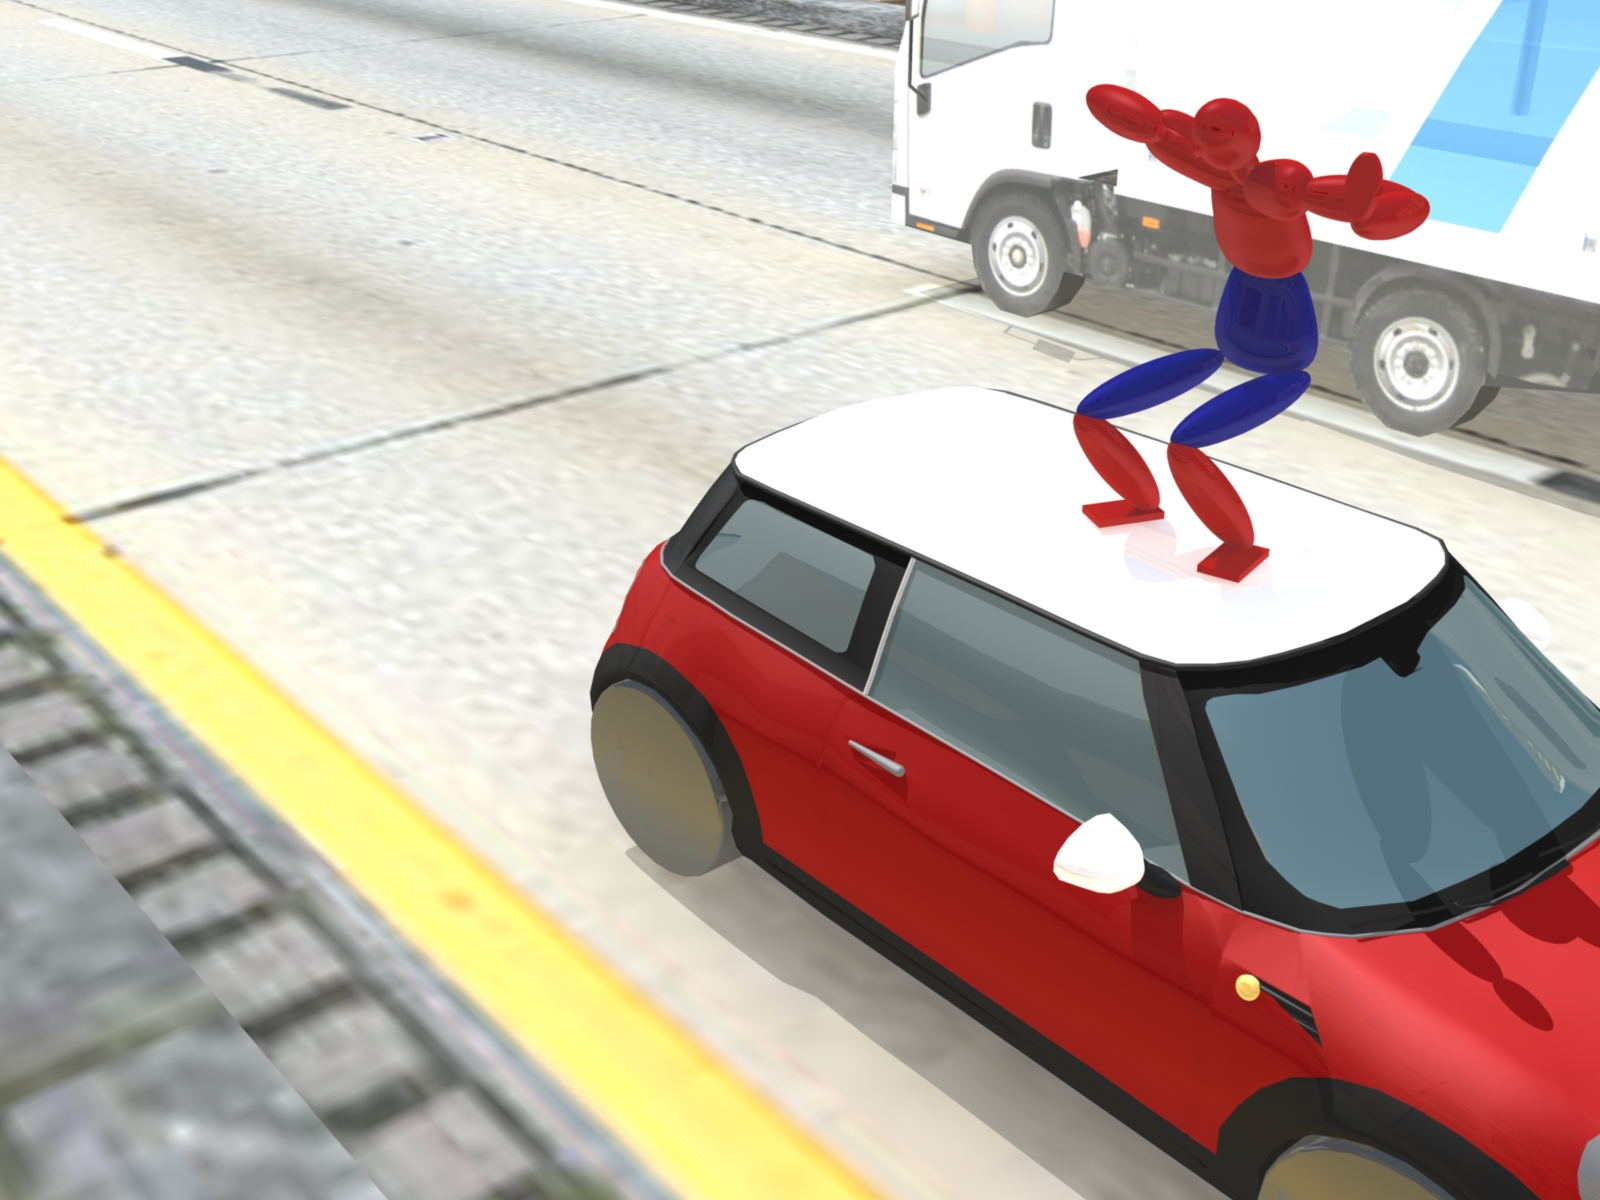
\includegraphics[width=0.48\textwidth]{images/intro_landing.jpg}
  \end{center}
   \vspace{-25pt}
  \caption{A falling motion of Parkour.}
  \label{fig:intro_landing}
   \vspace{-10pt}
\end{wrapfigure}
In Chapter 3, I will show how to create an on-line controller for generating 
agile and natural falling motions of the virtual character that can land from 
various heights and velocities.
The goals of the controller are to reduce the joint stress at the impact and
get back on its feet to prepare the next action.
Inspired by falling skills of Parkour(\figref{intro_landing}), I formulate the falling problem
with three phases, \emph{airborne}, \emph{impact}, and \emph{rolling}
based on the contact states.
First, two sub-controllers are designed for the \emph{airborne} and
\emph{rolling} phases and a regression analysis is conducted to find 
an optimal landing angle that can connect two sub controllers at the
\emph{impact} phase.
I will demonstrate that the motion generated by the proposed controller
induces smaller joint stress, which is still four times lower than a rag-doll
motion at the worst cases.

\subsection{Multiple Contact Planning for Humanoids}
\begin{wrapfigure}{l}{0.5\textwidth}
 \vspace{-25pt}
  \begin{center}
    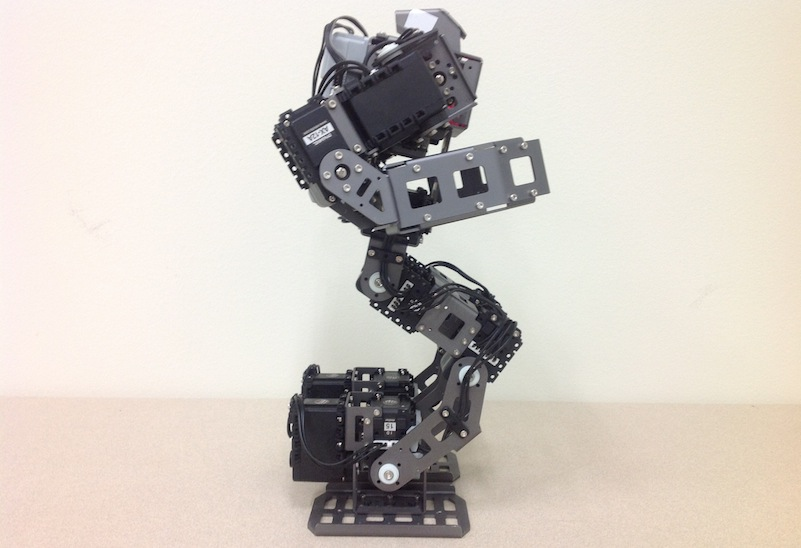
\includegraphics[width=0.48\textwidth]{images/intro_hardware.jpg}
  \end{center}
   \vspace{-25pt}
  \caption{Hardware of BioloidGP robot.}
   \vspace{-10pt}
  \label{fig:intro_hardware}
\end{wrapfigure}
% Goal, Method (Strength), Verification + Image
Chapter 4 will describe a general algorithm which plans for appropriate 
responses to a wide variety of falls, from a single step to recover a gentle nudge, to a rolling motion to break a high-speed fall.
Our multiple contact planning provides a unified framework
that can represent many existing falling techniques [,,].
Then, I will show how to efficiently optimize the multiple contact falling
strategy to the given initial state using a simplified model and dynamic 
programming.
Finally, various scenarios will be tested on simulated humanoids and the
actual hardware (\figref{intro_hardware}) to show that our algorithm plans
various falling strategies with different contact sequences.

\section{Learning of Dynamic Controller for Characters}
% Introduction on the learning - Motivation, Description, Goal
Teaching a physically simulated character a new motor skill requires 
a lot of efforts from the controller designer, from the design of the control 
mechanism to the tweaking of low-level control parameters.
To simplify the learning process, I will introduce an intuitive and 
interactive framework for developing dynamic controllers that is inspired by
how humans learn dynamic motor skills through a iterative process of coaching
and practicing.
Further, we propose two optimization techniques that can extend the popular
policy search algorithm, CMA-ES, to accelerate the convergence rate
and to optimize a parametrized objective function.

\subsection{Iterative Design of Dynamic Controllers}
% Goal, Method (Strength), Verification + Image
\begin{wrapfigure}{r}{0.6\textwidth}
 \vspace{-10pt}
  \begin{center}
    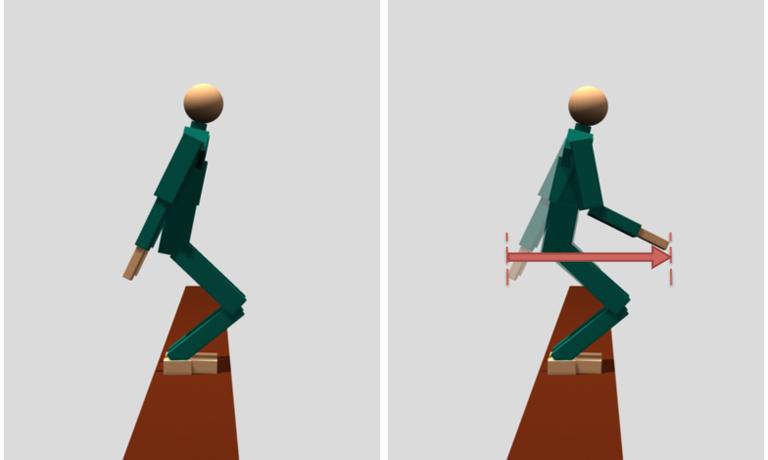
\includegraphics[width=0.58\textwidth]{images/intro_teach.png}
  \end{center}
   \vspace{-25pt}
  \caption{The proposed learning frame uses human readable instructions
    to teach motions.}
  \label{fig:intro_teach}
   \vspace{-10pt}
\end{wrapfigure}
In Chapter 5, I will describe an iterative framework to design dynamic
controllers using high-level, human-readable instructions,
inspired by a training process of athletes that consists of
interactive coaching and repetitive practices (\figref{intro_teach})
To enable interactive coaching, I introduce ``control rigs'' as
an intermediate layer of control module to facilitate the mapping between
human instructions and low-level control parameters.
During the practicing stage, control parameters are efficiently determined
using CMA-ES, which will be further improved in the following chapters.
The details of controllers development process using our iterative learning
framework will be shown with example parkour motions.

\subsection{Optimization with Failure Learning}
% Goal, Method (Strength), Verification + Image
A controller with many user constraints is difficult to optimize due to the
relatively small feasible region.
In Chapter 6, I will describe a new optimization algorithm based on the
observation of human’s ability to learn from failure.
The proposed algorithm, CMA-C (Covariance Matrix Adaptation with
Classification) utilizes the failed simulation trials to approximate 
an infeasible region in the space of control rig parameters, resulting a
faster convergence than the standard CMA-ES.

\subsection{Optimization for Parametrized Motor Skills}
% Goal, Method (Strength), Verification + Image
In Chapter 7, I will show how to optimize parametrized motor skills that are
essential for autonomous robots operating in an unpredictable environment. 
By evolving a parametrized probability distribution, the algorithm reduces 
the number of samples required to optimize a parametrized skill for 
all the tasks in the range of interest. 

\section{Model-based Learning for virtual and real characters}
% Introduction on the bias

\section{Contributions}
The control and optimization methods discussed in this dissertation provide
several contributions to the computer animation community. 
These contributions are as follows:


\begin{itemize}
\item \textbf{A falling and landing strategy for various initial conditions}
  The algorithm presented in the dissertation allows the character to fall from 
  a wide range of heights and initial speeds, continuously roll on the ground, 
  and get back on its feet, without inducing large stress on joints at any
  moment.
\item \textbf{A multiple contact falling strategy for humanoids}
  We introduce a new planning algorithm to minimize the damage of humanoid 
  falls by utilizing multiple contact points. 
\item \textbf{An iterative learning framework for dynamic motor skills}
  Inspired by how humans learn dynamic motor skills through progressive process 
  of coaching and practices, we introduce an intuitive and interactive 
  framework for developing dynamic controllers. 
\item \textbf{An optimization technique that utilized failed samples}
  We introduce a novel efficient optimization algorithm, CMA-C, that shows 
  that faster convergence rate by approximating the infeasible region of a  
  particular type of failure with Supported Vector Machines.
\item \textbf{An optimization technique for parametrized objectives}
  We introduces an efficient evolutionary optimization algorithm for learning
  parametrized skills to achieve whole-body dynamic tasks. 
\end{itemize}


%1234567890123456789012345678901234567890123456789012345678901234567890123456789
\chapter{Introduction}

The human desire to be physically impressive has a long history which can be
dated back to ancient Greece.
The ancient Olympic Games celebrated the glory of physical dominance of
athletic strength and agility, to achieve the goals faster and more
effortlessly. 
In modern days, physical agility continue to captivate our imagination in
various areas, such as sports, entertainments, or robots.
In the film or game industries, agile motions are important contents to make
their games or movies more fun and entertainings, from an iconic game
Prince of Persia [PP] to a recent big hit animation, Frozen [FR].
Besides entertainment values, being agile and strong also holds great practical
values, such as recovering disaster scenes with robots.
When there was a nuclear melt down that was too dangerous to be recovered
by human due to high radiation levels, few robots were entered to measure
temperature and radioactivity but failed due to limited speed and range of
operations [WIKIPEDIA].
Although even the state-of-arts humanoids are not as agile as human athelets
or virtual characters in animations, their software and hardware specification
have made substantial progress in past few dacades and will have enough agility
to execute athletic motor skills in near future.

Although the word ``agile'' has similar meaning in everyone's mind,
it needs a more clear definition to be discussed in this dissertation.
According to many dictionaries [DICT], the language definition of ``agile''
is ``able to move quickly, easily, effortlessly, and gracefully.''.
It is more straightforward to associate a concrete physical meaning to the
first word ``quickly'' because its meaning can be directly mapped into
high momentum.
However, the other descriptors, ``easily'', ``effortlessly'', and
``gracefully'' are more difficult to be translated because they can be due to
different reasons, such as the innate strengh of the subject, the accumulated
experience, or the ability to negotiate with the environment.
Instead of this loose verbal definition, I will use a narrow definition of the
word ``agile'' in the context of motions, ``able to move quickly and
effortlessly in a complex environment.'', which highlights torque efficiency
and well-coordinated strategies that exploits the environment.
Great examples of agile motions are motor skills of Parkour, such as
vaults, jumps, or flips which are developed to move from the current location
to destination in the most efficient path.
Those skills are well aligned with the previous definition because they are
executed with high linear and angular momentum, and planned to negotiate
environmental features such as walls, guard rails, or stairs. 

The aim of this dissertation is to design a set of computational tools to
develop agile motor skills on virtual and real humanoids.
Although the grand goal would be to achieve agile motor skills on humanoid
robots, but there are many unsolved practical issues to directly design aigle
motions on the hardware, such as delays, noises, or safety concerns.
Especially unlike biped walking where adequate models and control theories are
already available, agile motions have not been studied extensively in the
literature of computer animation and robotics.
Thefore, the appropriate approach toward agile real humanoids is to first
develop theoretical models and control algorithms on the physics-based
simulation where researchers in compter graphics can accomplish complex and
stunning tasks, and then transfer the solution to the real hardware
with the careful adjustment.
Although there are intrinsic differences between virtual and real systems on
models, sensors, actuators, and so on, simulation-developed solutions will
greatly reduce the expensive cost of hardware experiments and prevent
unexpected dangerous situations.

Agile motor skills are difficult tasks for humanoids.
General characteristics of agile motions, high momentum or frequent changes
of contacts, increase difficulties of most existing issues in motor control
problems tremendously.
For instance, simple motion trajectories that are developed in virtual
simulation are more likely not to work on physical systems
because small errors can be quickly accumulated and result drastic deviations
from the original agile motions.
On the top of existing issues, agile motions generate few unique challenges
need to be addressed.
Unlikely well-defined motions such as running or reaching, agile motions cover
a wide range of diverse skills, such as jumping, vaulting, or rolling which are
governed by different control mechanisms and principals.
Because it is infeasible to manually design controllers for all tasks, we want
to develop a set of general tools for learning a variety of agile motions.
In addition, safety of humanoids must be ensured by learning how to fall
both intentionally and inadvertently, which are fundamental motor skills
required by various agile motions. 
These additional, unique challenges motivated me to address following problems
in this dissertation, as steps to achieve agile motions on virtual and real
humanoids.

\section{Falling Strategies for Humanoids}
% Introduction on the falling - Motivation, Description, Goal
Falling and landing motions are a set of fundamental motor skills
in various agile motions to protect humanoids themselves.
Because atheletic movements frequently involves
transitions between airborne and contact phases, they must know how to
absorb the shock at the landing moment and avoid damage to the body parts.
In addition, well-executed falling motions will lead a smooth transition to the
next motor skill. 
In this dissertation, I will discuss two different scenarios of fallings, 
for  virtual and real humanoids.
For a virtual humanoid, I will describe a physics-based controller that allows
the character to fall from a wide range of heights and initial speed, 
which are inspired by agile falling and landing of Parkour practioners.
For a real humanoid, I wiill propose a falling strategy for managing unexpected
falls due to a wide range of perturbations.
The effectiveness of both presented strategies are validated by measuring
amounts of joint stresses or contact forces to body parts in physics
simulation, and experimentally tested on a small-size humanoid.

\subsection{Falling and Landing Motion Control for Virtual Characters}
% Goal, Method (Strength), Verification + Image

In Chapter 3, I will show how to create a robust controller for generating 
agile and natural falling motions of the virtual character that can land from 
various heights and velocities.
The goals of the controller are to reduce the joint stress at the impact and
get back on its feet to prepare the next action (\figref{intro_landing}).

\begin{wrapfigure}{r}{0.5\textwidth}
 \vspace{-25pt}
  \begin{center}
    %% 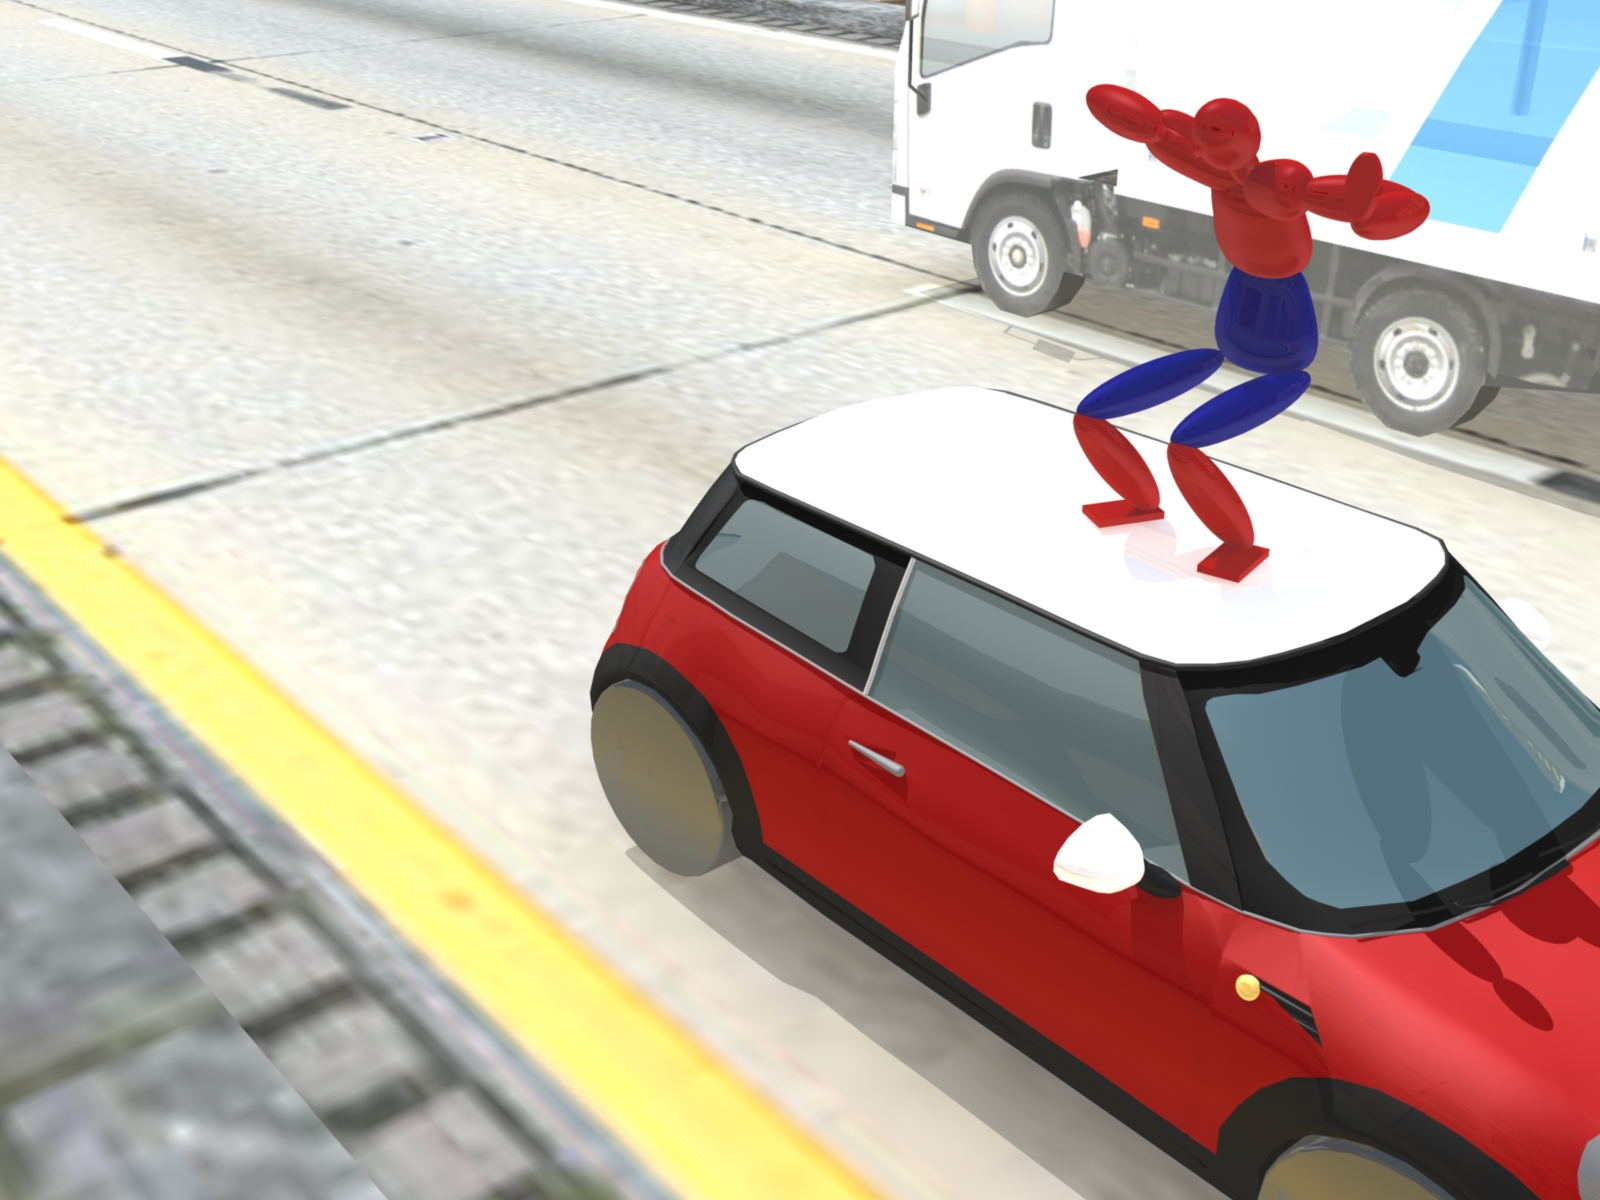
\includegraphics[width=0.48\textwidth]{images/intro_landing.jpg}
    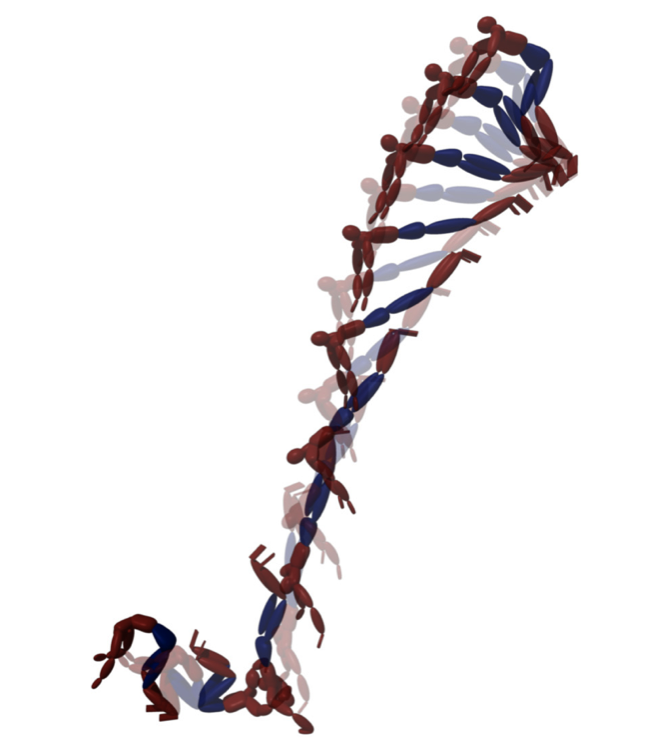
\includegraphics[width=0.48\textwidth]{images/intro_falling_sequence.png}
  \end{center}
   \vspace{-25pt}
  \caption{A fall of a virtual character.}
  \label{fig:intro_landing}
   \vspace{-10pt}
\end{wrapfigure}

Inspired by falling skills of Parkour, 
I formulate the falling problem
with three phases, \emph{airborne}, \emph{impact}, and \emph{rolling}
based on the contact states of a virtual character.
First, two sub-controllers are designed for the \emph{airborne} and
\emph{rolling} phases and a regression analysis is conducted to find 
an optimal landing angle that can connect two sub controllers at the
\emph{impact} phase.
I will demonstrate that the motion generated by the proposed controller
looks natural and induces smaller joint stress, which is still four times lower
than a uncontrolled rag-doll motion.



\subsection{Multiple Contact Planning for Humanoid falls}
\begin{figure}[h]
 %% \vspace{-25pt}
  \begin{center}
    %% 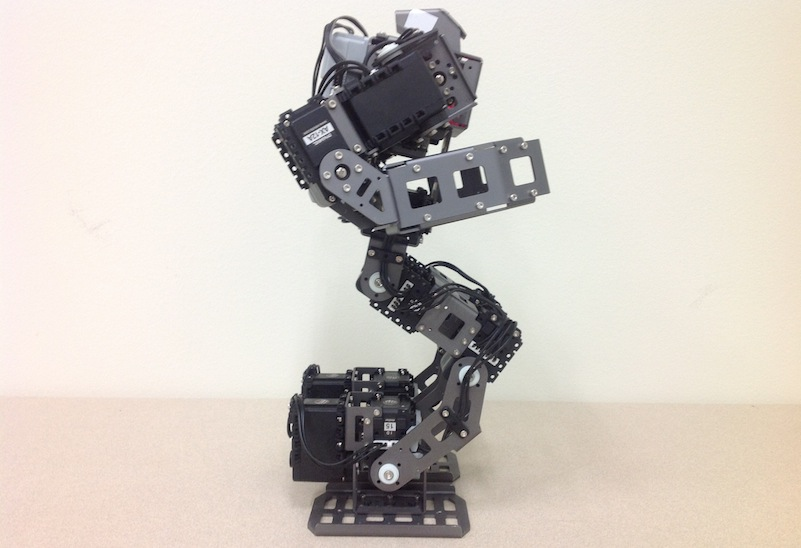
\includegraphics[width=0.48\textwidth]{images/intro_hardware.jpg}
    
\includegraphics[width=1.0\textwidth]{images/intro_gp_tripod}
  \end{center}
   %% \vspace{-25pt}
  \caption{A two-step falling strategy of a humanoid robot}
   %% \vspace{-10pt}
  \label{fig:intro_hardware}
\end{figure}
% Goal, Method (Strength), Verification + Image
Chapter 4 will describe a robust falling strategy which plans for appropriate 
responses to a wide variety of falls, from a single step to recover a gentle
nudge, to a rolling motion to break a high-speed fall.
Our key observation is that  many existing falling techniques [Wang,Yun,Ukemi]
assume specific sequences of contacts and aim to break specific ranges of
falls and requires us to an additional decision layer to choose the best
falling strategy to the given state.
Instead, our multiple contact planning algorithm provides a unified framework
for various existing falling strategies, which can adjust the number and order
of contact sequences with respect to different magnitudes of perturbations.
In the proposed continuous space of strategies, our algorithm can efficiently
find the best falling strategy for the given initial state using a simplified
model and dynamic  programming.
To verify our framework, a variety of scenarios are tested on simulated
humanoids and the actual hardware (\figref{intro_hardware}) to show that our
algorithm plans versatile falling strategies with different contact sequences.

\section{Learning of Dynamic Controller for Characters}
% Introduction on the learning - Motivation, Description, Goal
Unlikely well-defined tasks such as reaching or walking,
agile motions cover a wide range of diverse skills such as vaulting, flipping,
or rolling.
Because these agile motions are governed by different mechanisms and
principles, manually designing and fine-tuning specialized controllers for all
tasks is not a practical approach.
Design of an individual physics-based controller for a new motor skill is 
a time-consuming task  which requires a lot of manual efforts from the controller
designer, from the design of the control mechanism to the tweaking of low-level
control parameters. 
To simplify the costly learning process, I will introduce an intuitive and 
interactive framework for developing controllers that is inspired by
how humans learn dynamic motor skills through a iterative process of coaching
and practicing.
Another important component for the iterative controller design process
is an efficient optimization to reduce a turn-around time.
In this purpose, we propose two optimization techniques that can extend the
popular policy search algorithm, CMA-ES, to accelerate the convergence rate
and to optimize a parametrized objective function.

\subsection{Iterative Design of Dynamic Controllers}
% Goal, Method (Strength), Verification + Image
\begin{figure}[h]
 %% \vspace{-25pt}
  \begin{center}
    %% 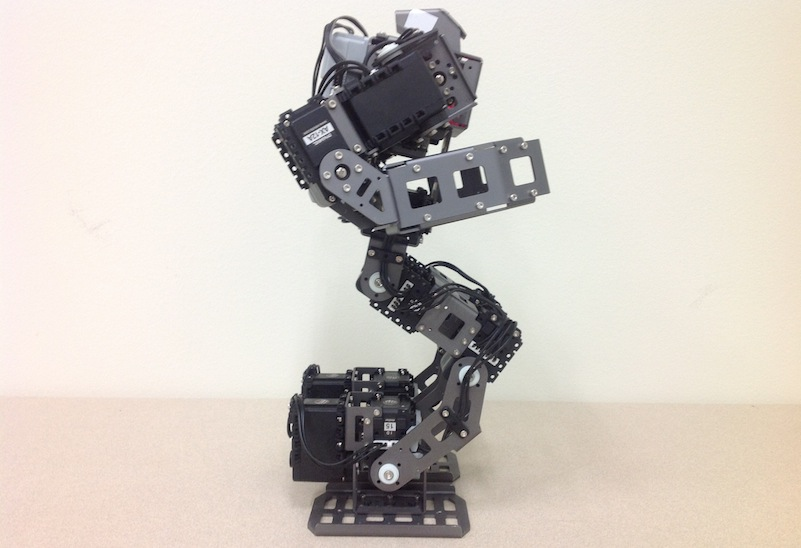
\includegraphics[width=0.48\textwidth]{images/intro_hardware.jpg}
    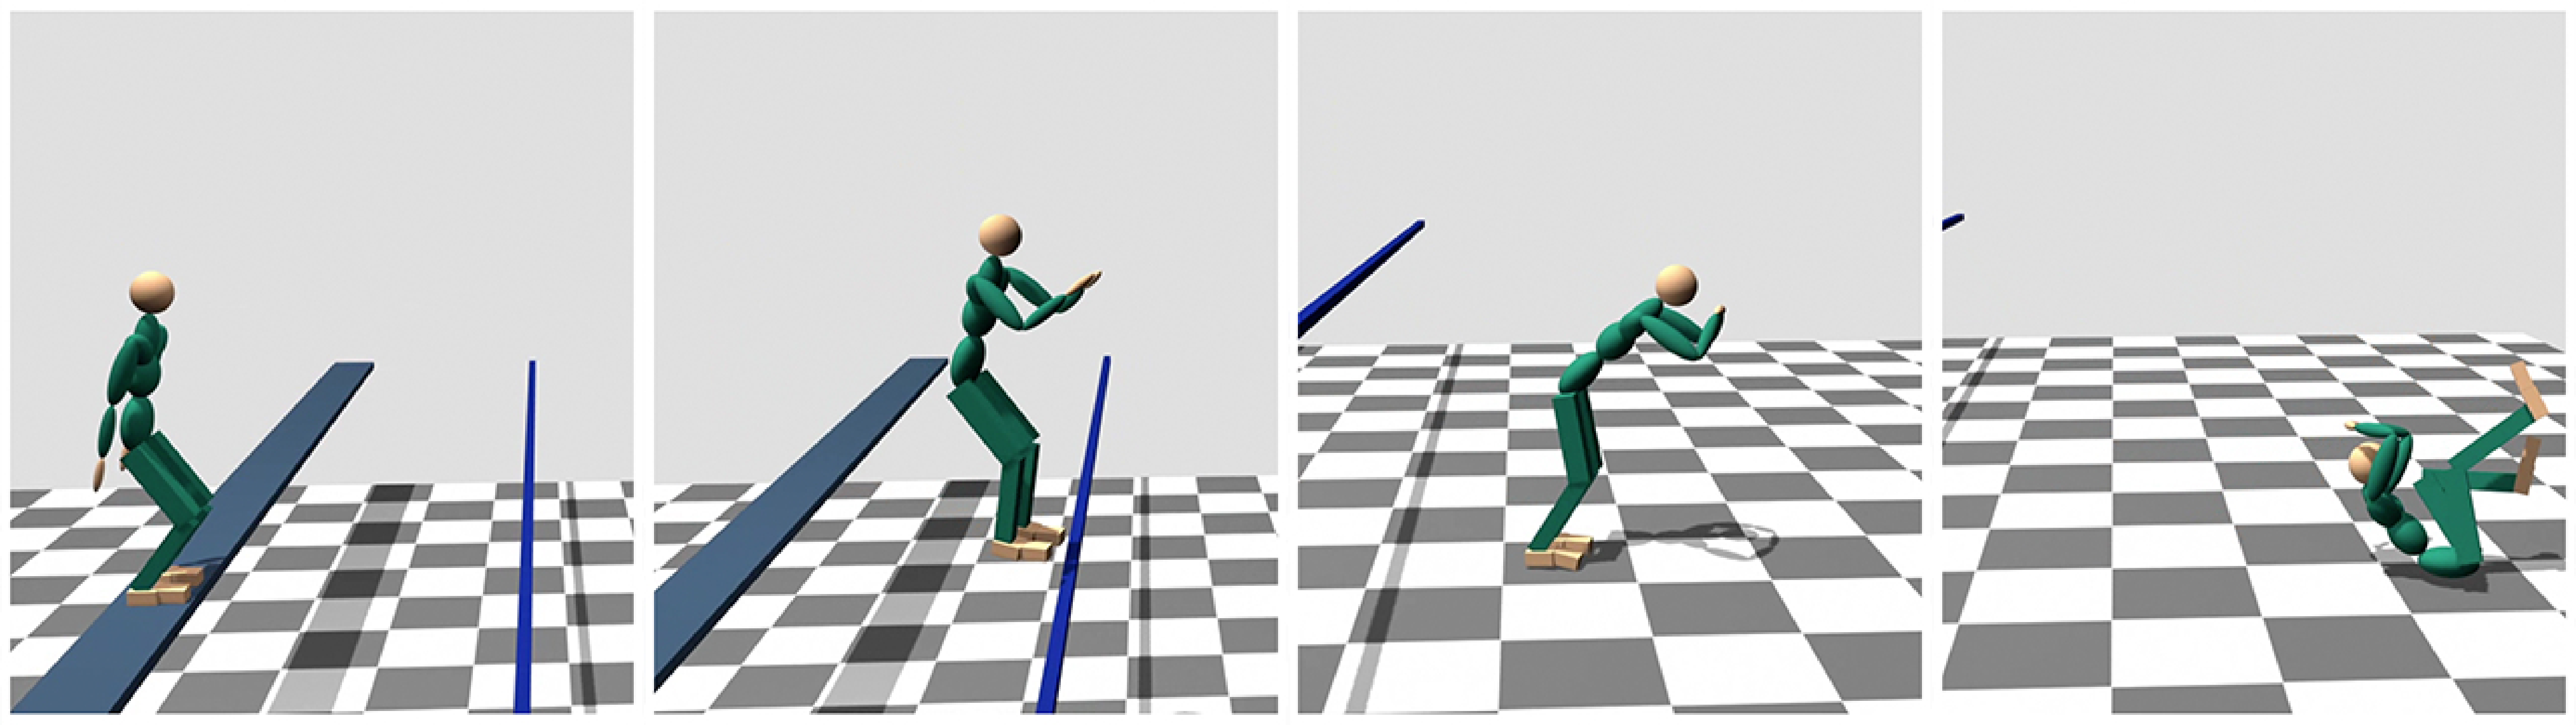
\includegraphics[width=1.0\textwidth]{images/intro_drop_roll}
  \end{center}
   %% \vspace{-25pt}
  \caption{A challenging stunt that a character jumps twice and rolls
    on the ground.}
   %% \vspace{-10pt}
  \label{fig:intro_drop_roll}
\end{figure}
%% \begin{wrapfigure}{r}{0.6\textwidth}
%%  \vspace{-10pt}
%%   \begin{center}
%%     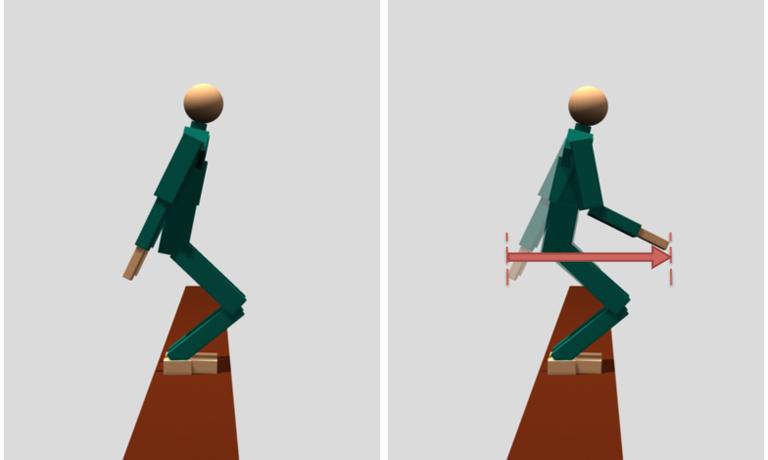
\includegraphics[width=0.58\textwidth]{images/intro_teach.png}
%%   \end{center}
%%    \vspace{-25pt}
%%   \caption{The proposed learning frame uses human readable instructions
%%     to teach motions.}
%%   \label{fig:intro_teach}
%%    \vspace{-10pt}
%% \end{wrapfigure}

In Chapter 5, we will describe an iterative framework to design physics-based
controllers that executes very agile stunts (\figref{intro_drop_roll}).
The aim of this chapter is to design an intuitive and interactive framework
that a user can easily design complex controllers only using high-level,
human-readable instructions, 
which is inspired by a human learning process of coaching and practicing stages.
To enable interactive coaching, we introduce ``control rigs'' as
an intermediate layer of control module which allows more coordinated control
of the low level control variables and and provides more intuitive mapping to
high-level human instructions. 
During the practicing stage, control parameters are efficiently determined
using CMA-ES, which will be further improved in the following chapters.
The details of controllers development process using our iterative learning
framework will be shown with example iterative training procedures of parkour
motions.

\subsection{Optimization with Failure Learning}
% Goal, Method (Strength), Verification + Image
In Chapter 6, I will describe a new optimization algorithm for
highly-constrained problems.
A controller with many constraints is difficult to be optimized due to the
relatively small feasible regions with many local minima.
Our key idea comes from human’s ability to learn from failure. 
Because failure in the real world is usually associated with pain or injury,
humans tend to be very effective in characterizing the cause of failure and
trying to avoid the same mistakes in the future. 
Under the concept of ``learning from failure'', The proposed algorithm CMA-C
(Covariance Matrix Adaptation with Classification) utilizes the failed
simulation trials to approximate an infeasible region in the space of control
rig parameters so that it can predict validities of newly generated samples,
resulting a faster convergence than the standard CMA-ES.

\subsection{Optimization for Parametrized Motor Skills}
% Goal, Method (Strength), Verification + Image
In Chapter 7, I will explain an evolutionary optimization algorithm for
learning parameterized skills to achieve whole-body dynamic tasks.
The parametrization of the learned motor skills is an essential ability
because a robot can reinterpret the skill to a new situation, without
learning the entire motor skill from scratch.
Instead of maintaining a single Gaussian distribution, 
the algorithm reduces the number of samples by evolving a parametrized
probability distribution which describes a mapping from a task parameter
to the optimal control parameters.
I will test the proposed optimization algorithm for learning three parametrized
dynamic motor skills on a simulated humanoid robot, including jumping,
kicking, and walking. 

\section{Model-based Learning for Virtual and Real Characters}
% Goal, Method (Strength), Verification + Images

In Chapter 8, I will describe an iterative approach for for learning 
hardware models and optimizing control policies, which is designed for
reducing the number of expensive hardware experiments.
Computer simulation is often used to replace hardware experiments,
but it is difficult to obtain accurate simulation models and
simulation-optimized control policies are not likely to work on hardware.
To fill the gap between two system, we propose an algorithm for learning
hardware models and optimizing policies. 
\begin{wrapfigure}{l}{0.5\textwidth}
 \vspace{-10pt}
  \begin{center}
    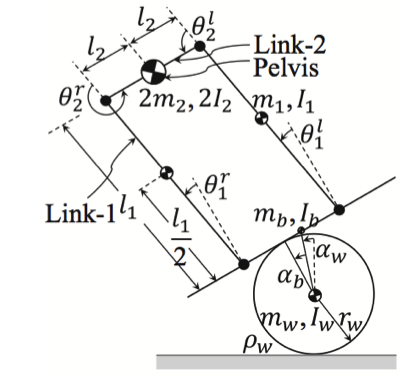
\includegraphics[width=0.40\textwidth]{images/intro_simple_robot.png}
  \end{center}
   \vspace{-25pt}
  \caption{A simple legged robot on the bongoboard.}
  \label{fig:intro_bongo}
   \vspace{-10pt}
\end{wrapfigure}
Instead of learning hardware models from scratch, the proposed approach only
learns the difference from a simulation model using Gaussian 
As a proof of concept, I will validate the algorithm on two different 
simulation models, one with perfect contacts and one with realistic contacts,
by finding a balancing controller for a simple bipedal robot on a bongo board
(\figref{intro_bongo}).

\section{Contributions}
The control and optimization methods discussed in this dissertation provide
several contributions to the computer animation and robotics community. 
These contributions are as follows:

\begin{itemize}
\item \textbf{A falling and landing strategy for virtual characters}
  The falling strategy presented in the dissertation generates a natural falling
  and landing motion that falls from a wide range of heights and initial
  speeds, continuously rolls on the ground, and gets back on its feet without
  inducing large stress on joints at any moment.
\item \textbf{A multiple contact falling strategy for robots}
  We introduce a falling strategy for humanoid robots which can break a
  fall with minimal damage to the body parts by optimizing the number and
  locations of contacts for the given initial state. 
\item \textbf{An iterative learning framework for dynamic motor skills}
  We propose an iterative and interactive learning framework 
  using human readable instructions that can teach a variety of agile motions
  to virtual characters.
  Starting from a basic controller, the proposed framework allows a user 
  to easily train complex physics-based controllers 
  with only intuitive high-level instructions from the user.
\item \textbf{An optimization technique for highly constrained problems}
  We introduce a novel efficient optimization algorithm, CMA-C, that is 
  designed for the problem with many constraints and smaller feasible regions.
  The algorithm converges faster than the standard CMA-ES,
  by approximating the infeasible region using learned classifiers.
\item \textbf{An optimization technique for parametrized tasks}
  We introduce an efficient evolutionary optimization algorithm for learning
  parametrized whole-body dynamic tasks.
  By evolving parameterized sample distributions, our algorithm
  converges faster than the baseline algorithm, CMA-ES.
\item \textbf{A model-based policy search for reducing hardware experiments}
  We propose an iterative approach for learning hardware model and optimizing
  policies with as few hardware experiments as possible by learning
  \emph{dynamics bias}, which is difference between simulation and hardware
  models. 
\end{itemize}

\rule{0.95\textwidth}{1pt}

In the next chapter, I will discuss the related work conducted by other
researchers to address similar problems.


%1234567890123456789012345678901234567890123456789012345678901234567890123456789
\chapter{Related work}

In this section, I will review the relevant previous work done in 
computer graphics, robotics, and bio-mechanics.
In \secref{related_dynamic}, I will start with a brief introduction on
popular character animation techniques to control highly dynamic motor skills
of biped characters in the physically simulated world.
In \secref{related_falling}, I will review previous methods for controlling
falling motions of humanoids to reduce damage to body parts.
In \secref{related_hitl}, I will briefly review an interactive design and 
optimization paradigm, \emph{human-in-the-loop optimization}, which is
adopted in this dissertation for incorporating interactive user interventions
in a controller design process.
Finally, I will review various policy search techniques and optimization
algorithms in both computer graphics and robotics, which are frequently
applied to the optimization of control parameters.

\section{Control of dynamic motor skills}
\label{sec:related_dynamic}

Previous work has demonstrated that highly
dynamic motions with a long ballistic phase can be synthesized using
physics simulation or kinematic approaches. Hodgins \etal
\cite{Hodgins:1995:AHA,Wooten:1998:Phd} showed that carefully
crafted control algorithms can simulate highly athletic motions,
including diving, tumbling, vaulting, and leaping. Faloutsos \etal
\cite{Faloutsos:2001:CCF} composed primitive controllers to
simulate more complex motor skills, such as a kip-up move or a dive
down stairs. Liu \etal \cite{Liu:2010:SCM} successfully tracked
contact-rich mocap sequences using a sampling-based approach. They
showed that vigorous motions with complex contacts, such as a
dive-roll or a kip-up move, can be dynamically simulated, provided
full body mocap sequences as desired trajectories. Zhao and van de
Panne \cite{Zhao:2005:UII} provided a palette of parametrized
actions to build a user interface for controlling highly dynamic
animation.  Other techniques directly edit ballistic motion sequences
under the constraints imposed by conservation of momentum
\cite{Majkowska:2007:FPM,Sok:2010:EDH}, or apply a hybrid method for
synthesizing dynamic response to perturbation in the environment
\cite{Shapiro:2003:HCI}.  If the contact positions and timing are
known, spacetime optimization techniques can also generate compelling
dynamic motions
\cite{Liu:2002:SCD,Fang:2003:ESP,Safonova:2004:SPR,Sulejmanpavic:2004:APB}.
In this dissertation, I take the approach of physical simulation, 
but I seek for a more general and robust control algorithm such that the
controller can operate under a wide range of initial conditions and
allow for runtime perturbations. 

Physics-based character animation is a promising approach to creating
realistic and interactive animations, but designing controllers
remains difficult largely due to the complex relationship between the
control and the state variables. Early work
\cite{Hodgins:1995:AHA,Wooten:1998:Phd} demonstrated that a variety of
motions can be achieved by controlling the individual joints with
manually designed state machines. Since this seminal work was
published, researchers in computer animation have been searching for
new control algorithms that are more robust, more generalizable, and
more automatic. Using motion capture data for reference
trajectories was a step toward a more automatic process for controller
design 
\cite{Zordan:2005:DRM,Sok:2007:SBB}, 
however, the simulated motions
cannot deviate much from the input data. An improved approach applied
linear or nonlinear quadratic regulators to track reference
trajectories, leading to more robust controllers against perturbations
\cite{daSilva:2008:ISS,Muico:2009:CNC}. Combination of PD servos and a
specialized balance controller driven by a simple state machine was a
very successful strategy \cite{Yin:2007:SIM}, which enabled much
follow-on work in biped control 
\cite{Wang:2009:OWC,Coros:2010:GBW,Lee:2010:DDB,Jain:2011:CPC}. 
Global planning of momentum
has also been applied to a wide range of motion from standing balance
\cite{Macchietto:2009:MCB} to locomotion 
\cite{Mordatch:2010:RPL,Ye:2010:OFC}
to highly dynamic motion 
\cite{Ha:2012:FAL,Liu:2012:TRC,AlBorno:2013:TOF,Zordan:2014:CRD}
Coros \etal adopted Jacobian transpose control from robotics literature
\cite{Sunada:1994:ACJ} to generate stable biped and quadruped
locomotion \cite{Coros:2010:GBW,Coros:2011:LSS}. Ha \etal further
demonstrated the effectiveness of the Jacobian transpose control on
dynamic stunts 
\cite{Liu:2010:SCM,Ha:2012:FAL,Ha:2014:ITD}.



\section{Control of falling motions}
\label{sec:related_falling}

\subsection{Falling detection techniques}
To activate a falling controller, a robot first predicts a fall and
try to recover the balance if it is possible.
Varioud machine learning techniques has been proposed to detect fall, such as
Principal Component Analysis \cite{Karssen:2008:FDW} or 
Supported Vector Machine \cite{Kim:2011:MLA}.
Horn and Gerth \cite{Hohn:2009:PBM} detects unstable situations with
Gaussian Mixture Model or Hidden Markov Model
and activates appropriate reflex controls, such as crouching. 
Renner and Benke \cite{Renner:2006:IDF} proposed to detect instability using
an aggregated sensor deviation and stabilize the gait with manually designed
reflex controllers. 
In this dissertation, 
I will focus on control of falling to reduce damage when the
robot detects falling, presumably with one of the above techniques. 

\subsection{Falling strategies for robots}
When falling is inevitable, various techniques has been proposed to
minimize damage on humanoid. 
Fujiwara \etal
\cite{Fujiwara:2002:UFM,Fujiwara:2003:FHH,Fujiwara:2006:TOF,Fujiwara:2007:OPF}
proposed falling techniques inspired by Japanese martial arts (\emph{Ukemi}).
Ogata \etal \cite{Ogata:2007:FMC,Ogata:2008:RSG} evaluates the risk of falling with
predicted ZMP and optimizes COM trajectories to reduce damage. 
Ruiz-del-Solar \etal \cite{Ruiz:2009:LTF,Ruiz:2010:FDM} designed low damage
falling sequences for soccer robots and verified them in the simulation. 
Wang \etal \cite{Wang:2012:WTO} formulated an optimization of whole body
trajectories as a nonlinear programming problem and solved it with heuristics.
Lee and Goswami \cite{Lee:2012:FOB} proposed a control strategy that
reorients the robot to fall with a backpack for absorbing shock. 
Yun and Goswami \cite{Yun:2014:TFC} addressed a ``tripod'' strategy that
stops with a swing foot and two hands to maintain the final COM location
higher from the floor.   
To protect the surrounding environment, \cite{Goswami:2014:DCF} proposed a
fall direction-changing strategy that utilizes foot placement and inertia
shaping.
% However, most of falling strategies assume the specific sequence of contacts
% that is specialized to the given scenarios, such as ``hands''
% \cite{Ogata:2007:FMC}, ``knee-and-hands'' \cite{Fujiwara:2007:OPF}, or
% ``foot-and-hands'' \cite{Yun:2014:TFC}. 

\subsection{Falling strategies for long-airborne scenarios}
In contrast to the related work in robotics, 
there are more works that focus on falls from higher
places. In those cases, control strategies during long airborne phase
become critical for safe landing. We draw inspiration from
kinesiology literature and sport practitioners. In particular, the
techniques developed in freerunning and parkour community are of
paramount importance for designing landing control algorithms capable
of handling arbitrary scenarios
\cite{Edwardes:2009:TPF,HLJ:2011:URL}. 
In robotics, \cite{Bingham:2014:OMA} \etal proposed an algorithm 
that leverages nonholonomic trajectory planning inspired by the
falling cat to orient an articulated robot through configuration
changes to achieve a pose that reduces the impact at landing.

\subsection{Falling strategies of animals}
Many animals have astonishing capabilities to achieve different
maneuvers in the air by manipulating their body articulations.  Cats
are known for landing with feet from any initial falling condition
\cite{Kane:1969:DEF,Montgomery:1993:GTF}. Lizards swing their tails to
stabilize their bodies during a leap \cite{Libby:2012:TAP}. Pigeons
reorient their bodies to achieve a sharp turn when flying at low speed
\cite{Ros:2011:PSL}. These behaviors inspire scientists and engineers
to develop intelligent devices and control algorithms. Our work has a
similar goal that we study how human body can change shape in the
air to reduce damage at landing.

\section{Human-in-the-loop design principle}
\label{sec:related_hitl}

\subsection{Human-in-the-loop interfaces}
Without human guidance, fully automated optimization algorithms
sometimes produce undesired solutions due to unmodelled factors or
unexpected situations. To fill the gap, researchers have developed
semi-automatic systems which involve a human in the process to provide
prior knowledge and guidance to the
optimization.
\cite{Scott:2002:IHC}. 
%% To compensate this issue, human-in-the-loop (HITL) optimization systems
%% \cite{Anderson:2000:HGS,Scott:2002:IHC,Klau:2010:HGS} have been
%% developed to model 
This type of optimization systems, called human-in-the-loop (HITL)
optimization, have proven effective for various problems, such as
%% space shuttle scheduling \cite{Chien:1999:APS}, 
vehicle planning
\cite{Waters:1984:IVR} or interface optimization
\cite{Quiroz:2007:IEX}.  The level of user interaction
varies from simply selecting of the generated solutions
\cite{Sims:1991:AEC} to directly editing the search parameters and
constraints \cite{Sreevalsan-Nair:2007:HGE}. Unlike
most previous work which primarily focused on developing user
interaction and visualization techniques for HTIL optimization
systems, we develop new optimization algorithms that exploit the nature of
HITL computation paradigm.


\subsection{Parameter selection interfaces}
A common approach in parameter selection interfaces is to present the parameter space (or a collection of samples thereof) in an explorable way,
through 2D layout of results \cite{Marks:1997:DGA};
careful selection of sliders \cite{Ovsjanikov:2011:Shapes,Lindow:2012:PLP};
or (in a physics context) direct manipulation \cite{Popovic:2000:IMR}
%Possibly cite mesh keyframing here as well
or in-situ visualization \cite{Twigg:2007:MWB}.
These methods help a designer understand the effects of parameter variation on a single set of initial conditions.
%%%%%%%%%%%%%%%%%%%%%%%%%%%%%%%%%%%%%%%%%%%%%%%%%%%%%%%%%%%%
% Newly updated related section
Both \cite{WFR:2010:WL,WFR:2011:NOR} represent simulations as tracks (or word lines) 
where each parameter change corresponds to branches that spawn new tracks, and 
\cite{WFR:2010:WL} describes how to incorporate uncertain parameter values into this explorable visualization.  
Meanwhile \cite{BM:2010:RDE} clusters outcomes from different timelines to suppress minor variations and to highlight entire outcome categories. 
As with other papers in this paragraph, 
our work is complementary as we can imagine deploying any of these techniques to specify and explore acceptable outcomes, 
while leaving our system to find consistent parameters over all the snapshots.



\section{Policy search algorithms}
\label{sec:related_policy}

\subsection{Model-free policy search}
Another approach is model-free policy optimization, where the policy is
improved through a number of hardware trials~\cite{bib-morimoto-standup,bib-kober-primitives}.
Unfortunately, these methods generally require hundreds of
trials, which is unrealistic for tasks such as humanoid balancing and
locomotion.
One way to overcome this issue is to limit the parameter space by using
task-specific primitives~\cite{bib-nakanishi-adaptation} or to provide a
good initial trajectory by human
demonstration~\cite{bib-atkeson-demonstration}.
However, it is not clear how to extend these approaches to dynamically
unstable robots or tasks that cannot described by joint trajectories.

\subsection{CMA-ES}
Various optimization techniques have been applied to improve the
motion quality or the robustness of the controller.  In character
animation, a sampling-based method, Covariance Matrix Adaption
Evolution Strategy (CMA-ES) \cite{Hansen:2004:CMA}, has been
frequently applied to discontinuous control problems, such as biped
locomotion \cite{Wang:2009:OWC,Wang:2010:OWC,Wang:2012:OLC},
parkour-style stunts\cite{Liu:2012:TRC,Ha:2014:ITD}, or swimming
\cite{Tan:2011:ASC}.  To compensate the expensive cost of
sampling-based algorithm, different approaches have been proposed,
including exploiting the domain knowledge
\cite{Wang:2009:OWC,Wang:2010:OWC,Wang:2012:OLC}, shortening the
problem horizons \cite{Sok:2007:SBB}, or using a classifier to exclude
infeasible samples \cite{Ha:2014:ITD}. Based on the previous success
of CMA-ES, we developed a new sampling-based algorithm resembles the
evolution process of distribution

\subsection{Model-based policy search}
Difference between a robot and its simulation model becomes a serious
problem when we try to use controllers obtained by model-based
optimization or tuned in simulation.
Classical parameter identification
techniques~\cite{bib-khalil-identification} partially solve this
problem by fitting model parameters to experimental data, but they
are still limited to factors that can actually be modeled. 
Furthermore, these approaches assume that the data set is large enough
to accurately estimate the parameters.
In large and unstable systems such as humanoid robots, it is often
difficult to collect enough data~\cite{bib-humanoids2011-calibration}.

A number of researchers have attempted to overcome the drawbacks of
these approaches by combining simulation and real-world data~\cite{bib-sutton-integrated,bib-moore-prioritized-sweeping,bib-peng-incremental}.
Abbeel et al.~\cite{bib-abbeel-inaccurate} used an inaccurate model to
estimate the derivative of the cost with respect to the policy
parameters.
Ko et al.~\cite{bib-ko-blimp} used Gaussian Process to model the
difference between a nonlinear dynamics model and the actual dynamics
and applied the model to reinforcement learning for yaw control of a
blimp.  However, they do not iterate the process to refine the model.
Deisenroth et al.~\cite{bib-deisenroth-data-efficient} also used
Gaussian Process for learning the dynamics model from scratch.
Similarly, Morimoto et al.~\cite{bib-iros07-improving} used Gaussian
Process for learning simplified dynamics of human locomotion.
Sugimoto et al.~\cite{bib-humanoid13-trajectory} used
\emph{sparse pseudo-input Gaussian Process} (SPGP) that accounts both
variances of inputs and outputs to handle sensor noises.
Instead, Tangkaratt et al.~\cite{bib-nn14-model} used 
\emph{least-squares conditional density estimation} (LSCDE) to learn 
the dynamics model without Gaussian assumption on the transitions.
Cutler et al.~\cite{bib-icra14-reinforcement} trained a policy in 
multiple fidelity simulators with discretized actions.
Ross and Bagnell~\cite{bib-ross-agnostic} theoretically proved that
their iterative system identification method converges even the system
is not in the assumed class.
Please refer to Section 6 of~\cite{bib-kober-survey} for more complete
survey on this topic.

\subsection{Skill generalization}
There is a large body of research work on generalization of learned
motor skills to achieve new tasks. da Silva \etal
\cite{DaSilva:2012:LPS,DaSilva:2014:LPM,DaSilva:2014:ACP} introduced a
framework to represent the policies of related tasks as a
lower-dimensional piecewise-smooth manifold. Their method also
classifies example tasks into disjoint lower-dimensional charts and
model different sub-skills separately. Much research aimed to
generalize example trajectories to new situations using dynamic
movement primitives (DMPs) to represent control policies
\cite{Ijspeert:2002:LAL}. A DMP defines a form of control policies
which consists of a feedback term and a feedforward forcing
term. Ude \etal \cite{Ude:2010:TSG} used supervised learning to train a set of
DMPs for various tasks and built a regression model to map task
parameters to the policy parameters in DMPs. 
Muelling \etal \cite{Muelling:2010:LTT}
proposed a mixture of DMPs and used a gate network to activate the
appropriate primitive for the given target parameters.
Kober \etal \cite{Kober:2010:RLA} trained a mapping between task parameters and
meta-parameters in DMPs using a cost-regularized kernel
regression. Through reinforcement learning framework, they computed a
policy which is a probability distribution over meta-parameters.
Matsubara \etal \cite{Matsubara:2011:LPD} trained a parametric DMP by shaping a
parametric-attractor landscape from multiple demonstrations.
Stulp \etal \cite{Stulp:2013:LCP} proposed to integrate the task parameters as
part of the function approximator of the DMP, resulting in more
compact model representation which allows for more flexible
regression. 
Neumann \etal \cite{Neumann:2013:IMS} modified the existing learning
algorithm (REPS) to learn a hierarchical controller that has
parameterized options.

All these methods described above depend on collecting a set of
examples. This presents a bottleneck to learning because an individual
control policy needs to be learned for each task example drawn from
the distribution of interest. da Silva \etal further proposed using
unsuccessful policies as additional training samples to accelerate the
learning process \cite{DaSilva:2014:LPM}. For dynamic motor skills
which involve intricate balance tasks, unsuccessful policies generated
during training a particular task are of no use to other tasks because
they often lead to falling motion. 
Hausknecht \etal \cite{Hausknecht:2010:LPK}
demonstrated a quadruped robot kicking a ball to various distances,
but whole-body balance was not considered in their work.  Another
challenge regarding dynamic tasks is that each task can be achieved by
a variety of policies, some of which might be overfitting the
task. Interpolating these overfitted policies can lead to unexpected
results. Our method tends to generate more coherent mapping between
task parameters and policy parameters because we simultaneously learn
the policies for the entire range of the tasks.

\chapter{Falling and Landing Motion Control for Virtual Characters}

\graphicspath{{landing/}}

\begin{figure}[ht]
\center
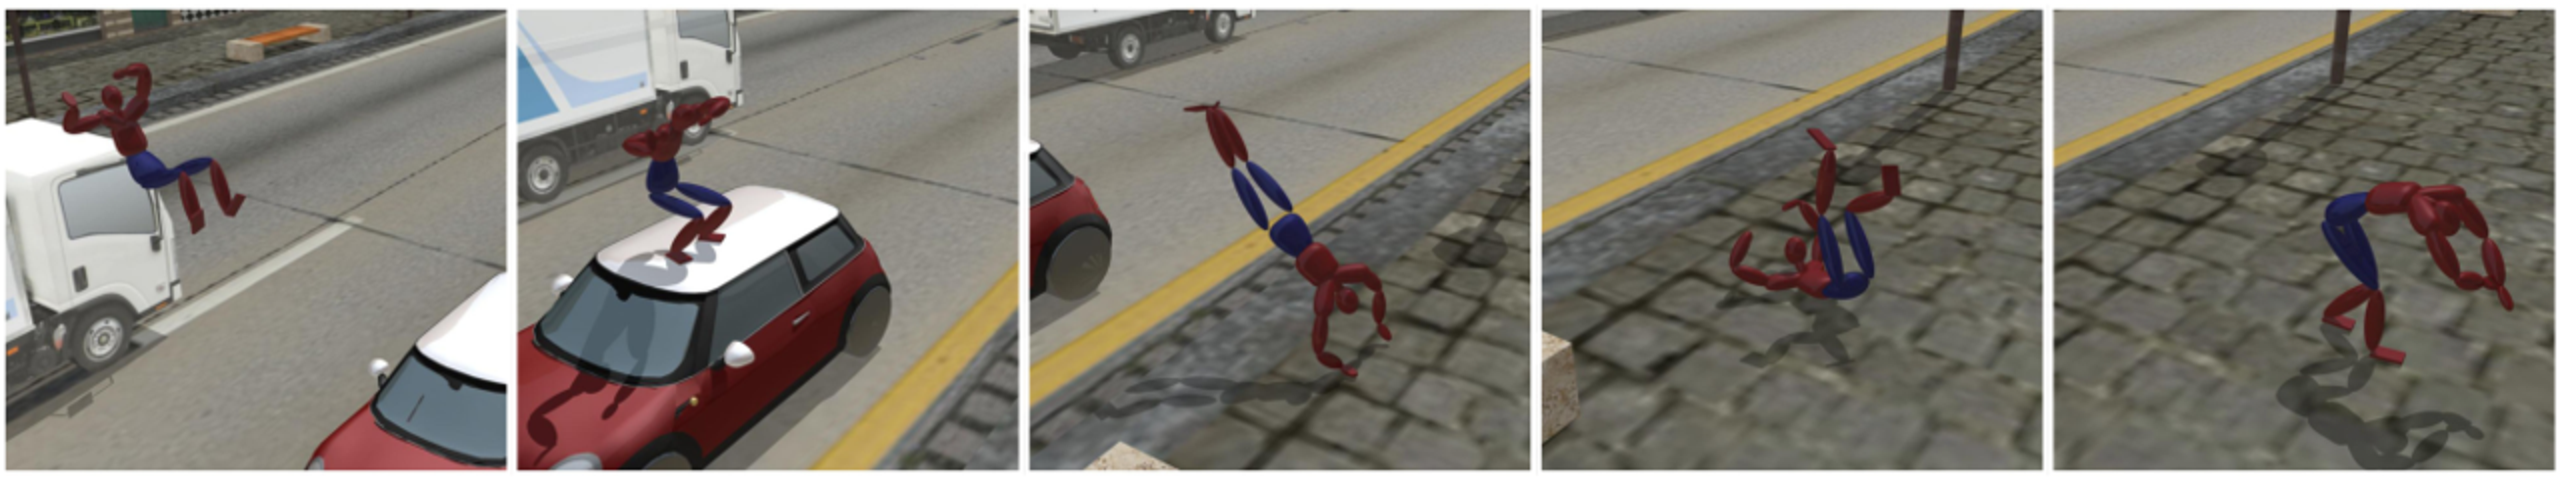
\includegraphics[width=\textwidth]{images/teaser2}
  \caption{A simulated character lands on the roof of a car, leaps
    forward, dive-rolls on the sidewalk, and gets back on its feet,
    all in one continuous motion.}
  \label{fig:landing_teaser}
\end{figure}

This chapter introduces 
a new method to generate agile and natural human landing
motions in real-time via physical simulation without using any mocap
or pre-scripted sequences. We develop a general controller that allows
the character to fall from a wide range of heights and initial speeds,
continuously roll on the ground, and get back on its feet, without
inducing large stress on joints at any moment. The character's motion
is generated through a forward simulator and a control algorithm that
consists of an airborne phase and a landing phase. During the airborne
phase, the character optimizes its moment of inertia to meet the ideal
relation between the landing velocity and the angle of attack, under
the laws of conservation of momentum. The landing phase can be divided
into three stages: impact, rolling, and getting-up. To reduce joint
stress at landing, the character leverages contact forces to control
linear momentum and angular momentum, resulting in a rolling motion
which distributes impact over multiple body parts. We demonstrate that
our control algorithm can be applied to a variety of initial
conditions with different falling heights, orientations, and linear
and angular velocities. Simulated results show that our algorithm can
effectively create realistic action sequences comparable to real world
footage of experienced freerunners.
\section{Motivation}
One of the great challenges in computer animation is to physically
simulate a virtual character performing highly dynamic motion with
agility and grace. A wide variety of athletic movements, such as
acrobatics or freerunning (parkour), involve frequent transitions
between airborne and ground-contact phases. How to land properly to
break a fall is therefore a fundamental skill athletes must acquire. A
successful landing should minimize the risk of injury and disruption
of momentum because the quality of performance largely depends on the
athlete's ability to safely absorb the shock at landing, while
maintaining readiness for the next action. To achieve a successful
landing, the athlete must plan coordinated movements in the air,
control contacting body parts at landing, and execute fluid
follow-through motion. The basic building blocks of these motor skills
can be widely used in other sports that involve controlled falling and
rolling, such as diving, gymnastics, judo, or wrestling.

We introduce a new method to generate agile and natural human
falling and landing motions in real-time via physical simulation
without using motion capture data or pre-scripted animation (Figure
\ref{fig:landing_teaser}). We develop a general controller that allows the
character to fall from a wide range of heights and initial speeds,
continuously roll on the ground, and get back on its feet, without
inducing large stress on joints at any moment. Previous controllers
for acrobat-like motions either precisely define the sequence of
actions and contact states in a state-machine structure, or directly
track a specific motion capture sequence. Both cases fall short of
creating a generic controller capable of handling a wide variety of
initial conditions, overcoming drastic perturbations in runtime, and
exploiting unpredictable contacts.

Our method is inspired by three landing principles informally
developed in freerunning community. First, reaching the ground with
flexible arms or legs provides “cushion” time to dissipate energy over
a longer time window rather than absorbing it instantly at impact. It
also protects the important and fragile body parts, such as the head,
the pelvis, and the tailbone. Second, it is advisable to distribute
the landing impact over multiple body parts to reduce stress on any
particular joint. Third, it is crucial to utilize the friction force
generated by landing impact to steer the forward direction and control
the angular momentum for rolling, a technique referred to as
"blocking" in the freerunning community. These three principles
outline the most commonly employed landing strategy in practice:
landing with feet or hands as the first point of contact, gradually
lowering the center of mass (COM) to absorb vertical impact, and
turning a fall into a roll on the ground, with the head tightly tucked
at impact moment.

However, translating these principles to control algorithms in
a physical simulation is very challenging. During airborne, the
controller needs to plan and achieve the desired first point of
contact and the angle of attack, in the absence of control over the
characters global motion in the air. Instead of solving a large,
nonconvex two-point boundary value problem, we develop a compact
abstract model which can be simulated efficiently for real-time
applications. To strike the balance between accuracy and efficiency,
our algorithm replans the motion frequently to compensate the
approximation due to the simplicity of the model. When the character
reaches the ground, the controller needs to take a series of
coordinated actions involving active changes of contact points over
a large area of human body. Our algorithm executes three consecutive
stages, impact, rolling, and getting-up by controlling poses,
momentum, and contacts at key moments. Furthermore, the airborne and
landing phases are interrelated and cannot be considered in
isolation: the condition for a successful landing defines the
control goals for the airborne phase while the actions taken during
airborne directly impact the landing motion. We approach this
problem in a reverse order of the action sequence: designing a
robust landing controller, deriving a successful landing condition
from this controller, and developing an airborne controller to achieve
the landing condition.


We demonstrate that our control algorithm is general,
efficient, and robust. We apply our algorithm to a variety of
initial conditions with different falling heights, orientations, and
linear and angular velocities. Because the motion is simulated in
real-time, users can apply perturbation forces to alter the course
of the character in the air. Our algorithm is able to efficiently
update the plan for landing given the new situations. We also
demonstrate different strategies to absorb impact, such as a dive
roll, a forward roll, or tumbling. The same control algorithm can be
applied to characters with very different body structures and mass
distributions. We show that a character with unusual body shape can
land and roll successfully.  
Finally, our experiments empirically showed that the algorithm induces
smaller joint stress, except for the contacting end-effectors. In
the worst case of our experiments, the average joint stress is still
four times lower than landing as a passive ragdoll.




\section{Overview}

We introduce a physics-based technique to simulate strategic falling
and landing motions from a wide range of initial conditions. Our
control algorithm reduces joint stress due to landing impact and
allows the character to efficiently recover from the fall. The
character's motion is generated through a forward simulator and a
control algorithm that consists of an \emph{airborne phase} and a
\emph{landing phase}. These two phases are related by an appropriate
\emph{landing strategy}, which describes the body parts used for the
first contact with the ground, a desired landing pose, and an ideal
landing condition that describes the relation between landing
velocities and the angle of attack in successful landing motions. We
develop two most common types of landing strategies: hands-first and
feet-first, and introduce a sampling method to derive the ideal
landing condition for each strategy.

\begin{figure}
\center
  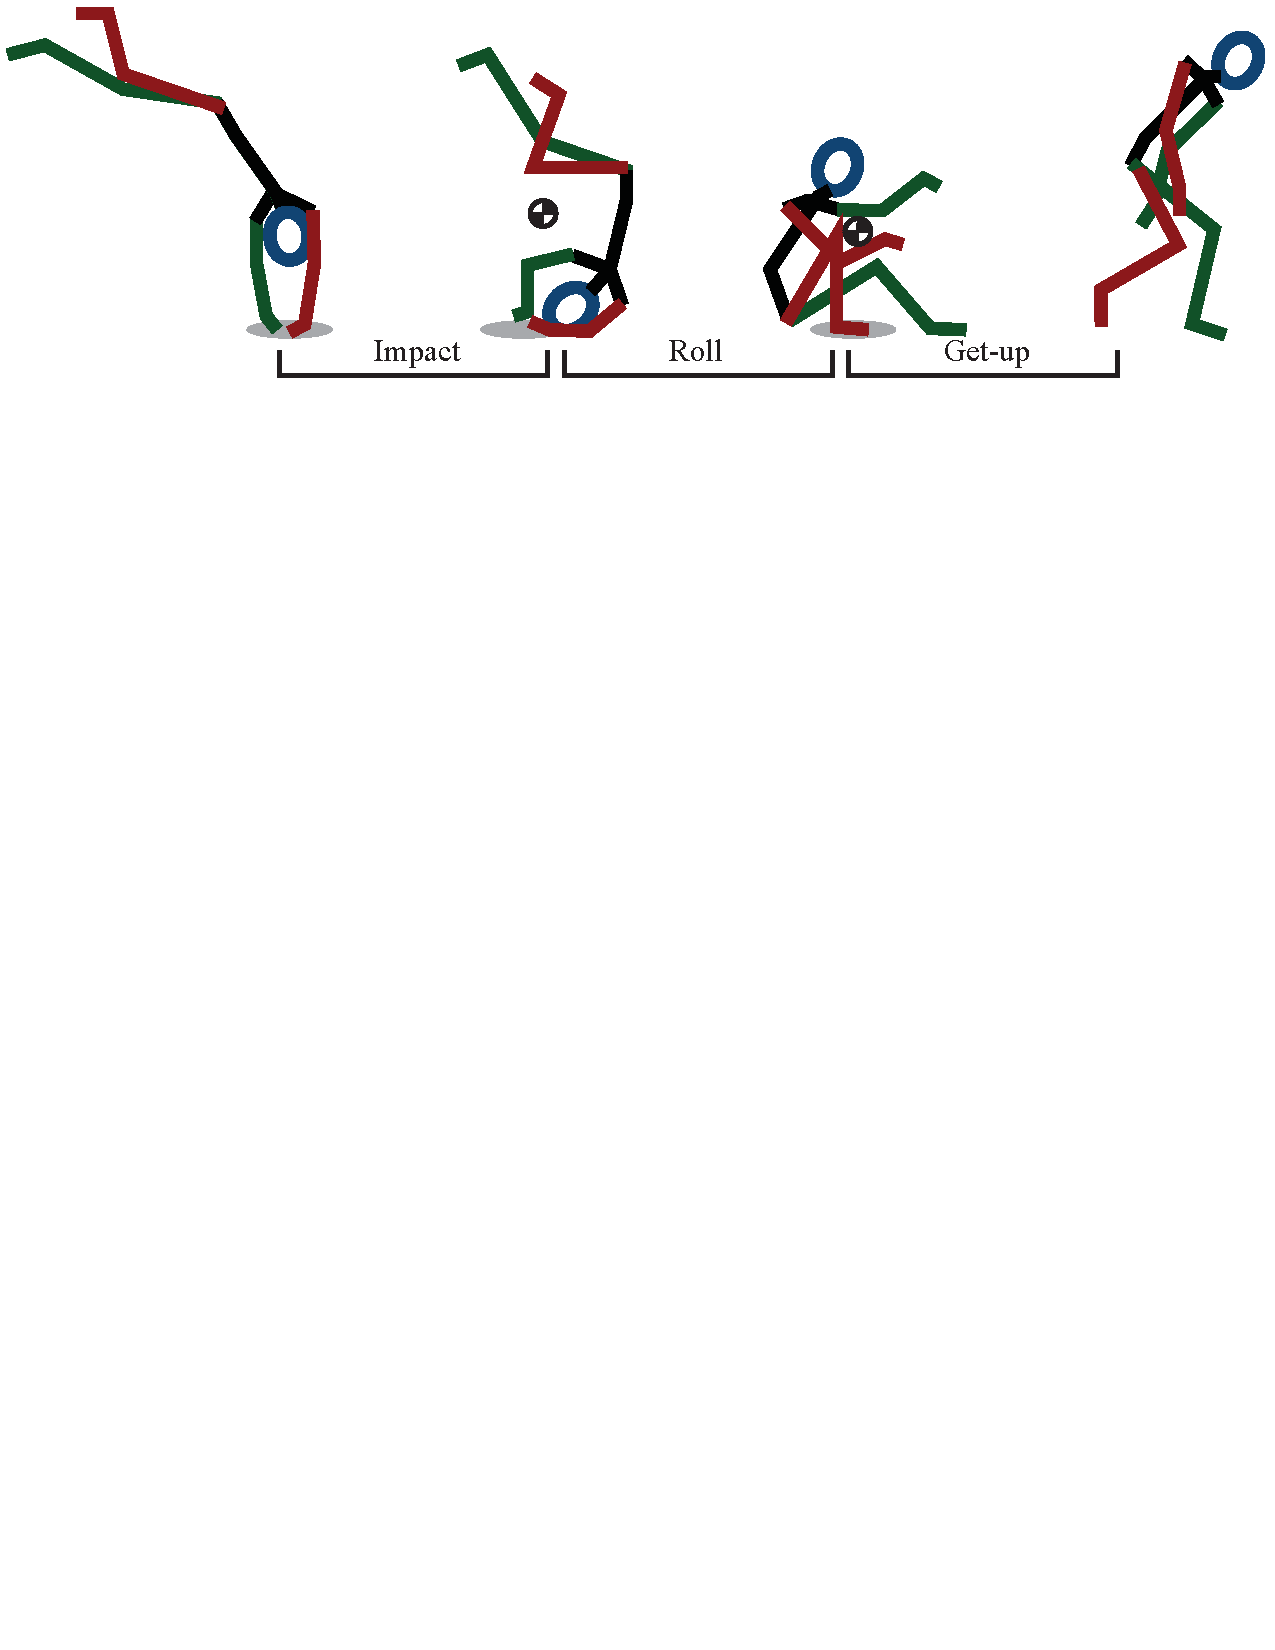
\includegraphics[width=4.2in]{images/landingPhase}
  \caption{Three stages in the landing phase.}
 \label{fig:landing_landingPhase}
\end{figure}

At the beginning of a fall, the character first decides on a landing
strategy. During the airborne phase, the character optimizes its
moment of inertia to achieve the ideal landing condition. The landing
phase is divided into three stages: impact, rolling, and getting-up
(Figure \ref{fig:landing_landingPhase}). The impact stage begins when the
character reaches the ground. 
%% During the impact stage, the character tries to control its linear 
%% and angular momentum while getting into a ready-to-roll pose. 
During the impact stage, the character leverages the friction forces 
from the ground to control linear and angular momentum. 
After the COM moves beyond the hand contact area,
the character switches to the rolling stage in which continuous change
of contact carries out. In preparation for standing up, the character
needs to maintain the rolling direction and plant its feet on the
ground. When the COM passes through the first foot, the character
starts to elevate the COM in order to compete the landing process in an
upright position.

\section{Landing Strategy}

Given an initial condition at the beginning of a fall, the character
can choose to land with the hands-first strategy or the feet-first
strategy.  In general, the hands-first strategy is chosen only for
aesthetics purpose because it is less robust and suitable only for
falls with planar angular momentum (about the pitch axis). In
contrast, the feet-first strategy can handle a wide range of arbitrary
initial conditions because it includes an extensive foot-ground
contact duration to modulate the momentum before rolling. A
landing strategy also includes a desired landing pose. Our algorithm
only requires a partial pose to stretch the arms or legs at landing,
depending on whether the hands-first or the feet-first strategy is
chosen. We manually specify this partial pose for each strategy
(\figref{landing_landingPoses}).


\begin{figure}[ht]
\center
  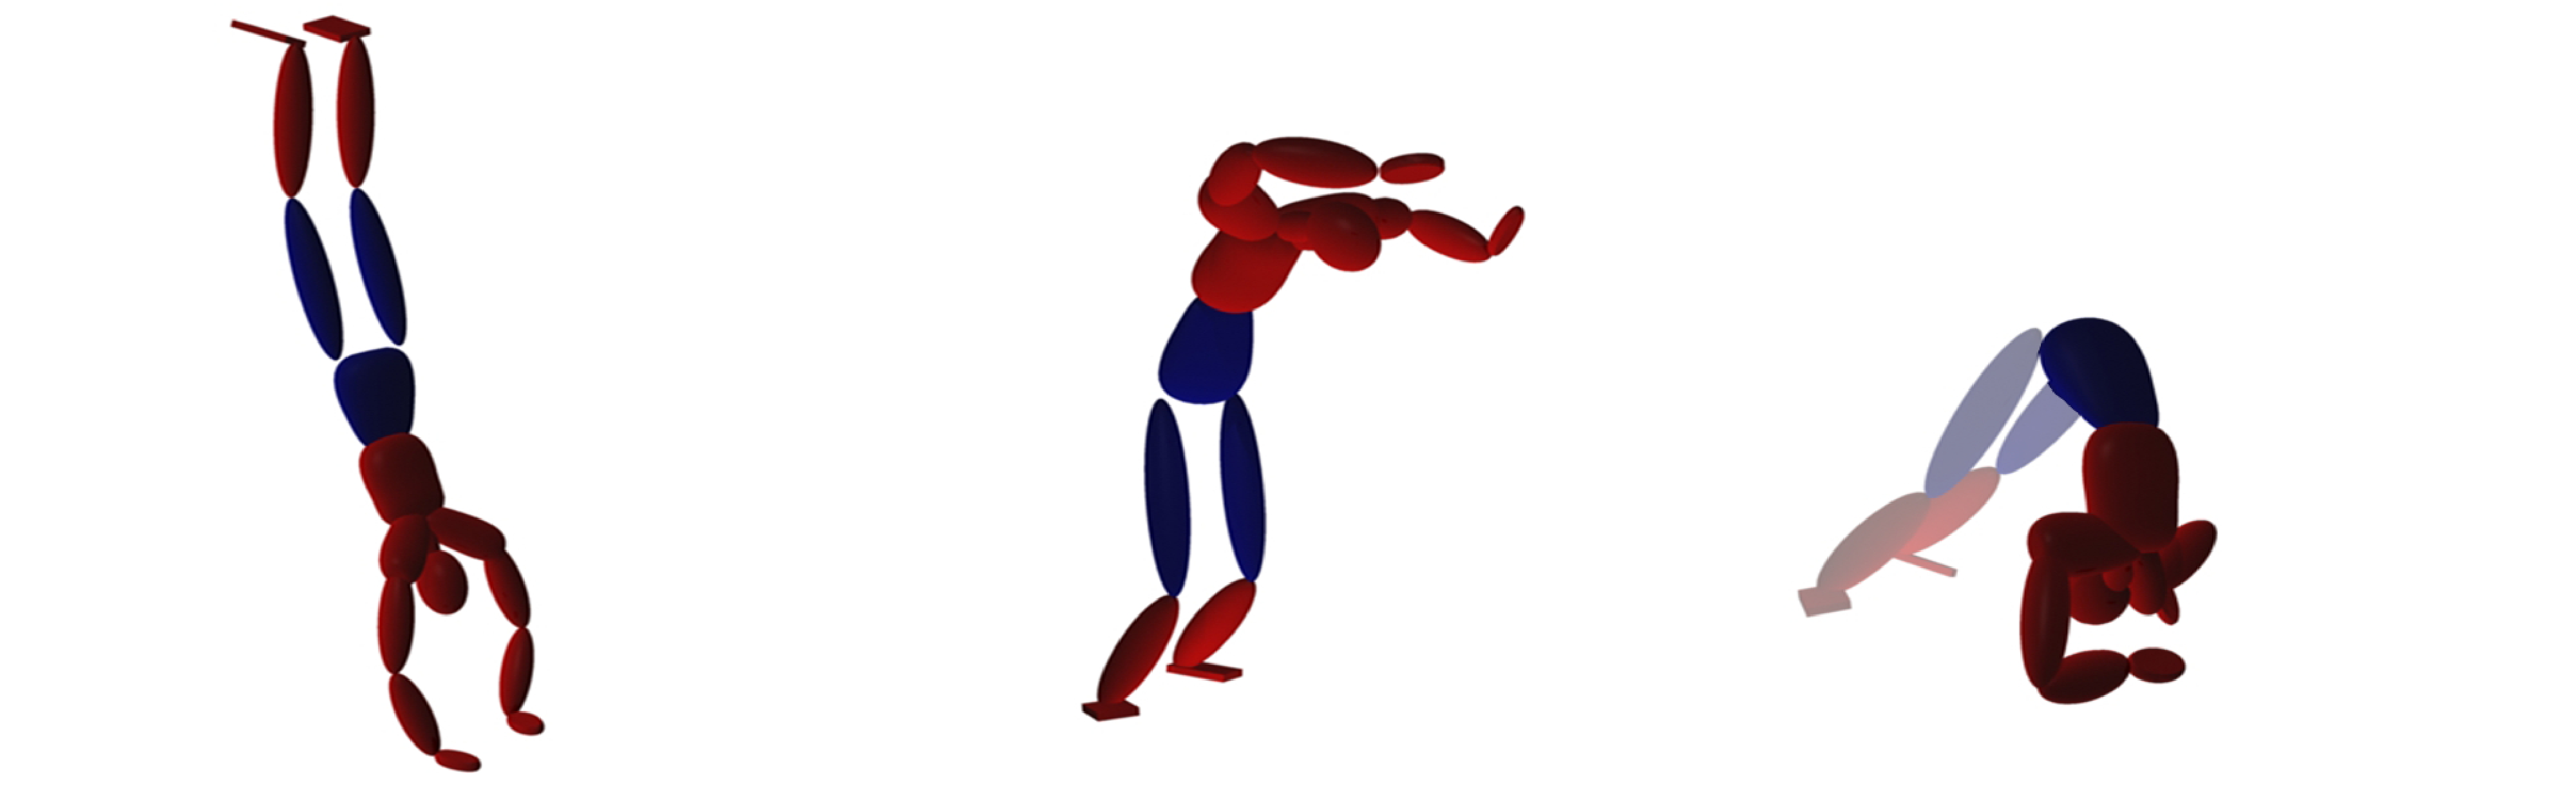
\includegraphics[width=3.2in]{images/LandingPoses}
  \caption{
    The left and middle are the desired landing poses for the
    hands-first strategy and the feet-first strategy, respectively.
    The right is the ready-to-roll pose for the feet-first strategy,
    which we track only the upper body.
  }
 \label{fig:landing_landingPoses}
\end{figure}

\begin{wrapfigure}{l}{0.5\textwidth}
  \begin{center}
    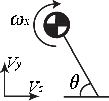
\includegraphics[width=0.28\textwidth]{images/COM}
  \end{center}
  \caption{\revised{Landing condition variables.}}
  \label{fig:landing_com}
\end{wrapfigure}

An integral part of our landing strategy is the landing condition, a
simple equation that compactly characterizes successful landing
motions.
\ignorethis{ A landing strategy describes an ideal landing
  condition key to the success of the subsequent rolling motion. We
  wish to derive a simple equation that compactly characterizes
  successful landing motions.} If the character manages to turn a fall
into a roll and gets back on its feet at the end of the roll, we
consider it successful.  Because a successful landing highly depends
on whether the character is able to control the momentum
at the moment of the first contact ($T$),
%% the character's momentum at the moment of first contact ($T$), 
our algorithm defines the landing condition as a relation between the
global linear velocity $\vc{v}^{(T)}$, global angular velocity
$\vc{\omega}^{(T)}$, and the angle of attack $\theta^{(T)}$, which
approximates the global orientation of the character
(\revised{\figref{landing_com}}).
The actual
coefficients of the landing condition depend on the design of the
landing controller, which cannot be derived analytically, but can be
learned from examples generated by the landing controller. We apply a
sampling method, similar in spirit to the approach Coros \etal
\cite{Coros:2009:RTC} presented for biped locomotion, to determine the
landing condition for a particular landing strategy.  \ignorethis{ A
  successful landing also depends on the design of the landing
  controller, which cannot be expressed in an analytical form.
  Therefore, we use a sampling approach to derive the relation,
  similar in spirit to the approach Coros \etal \cite{Coros:2009:RTC}
  presented for biped locomotion.}

\begin{figure}[ht]
\center
  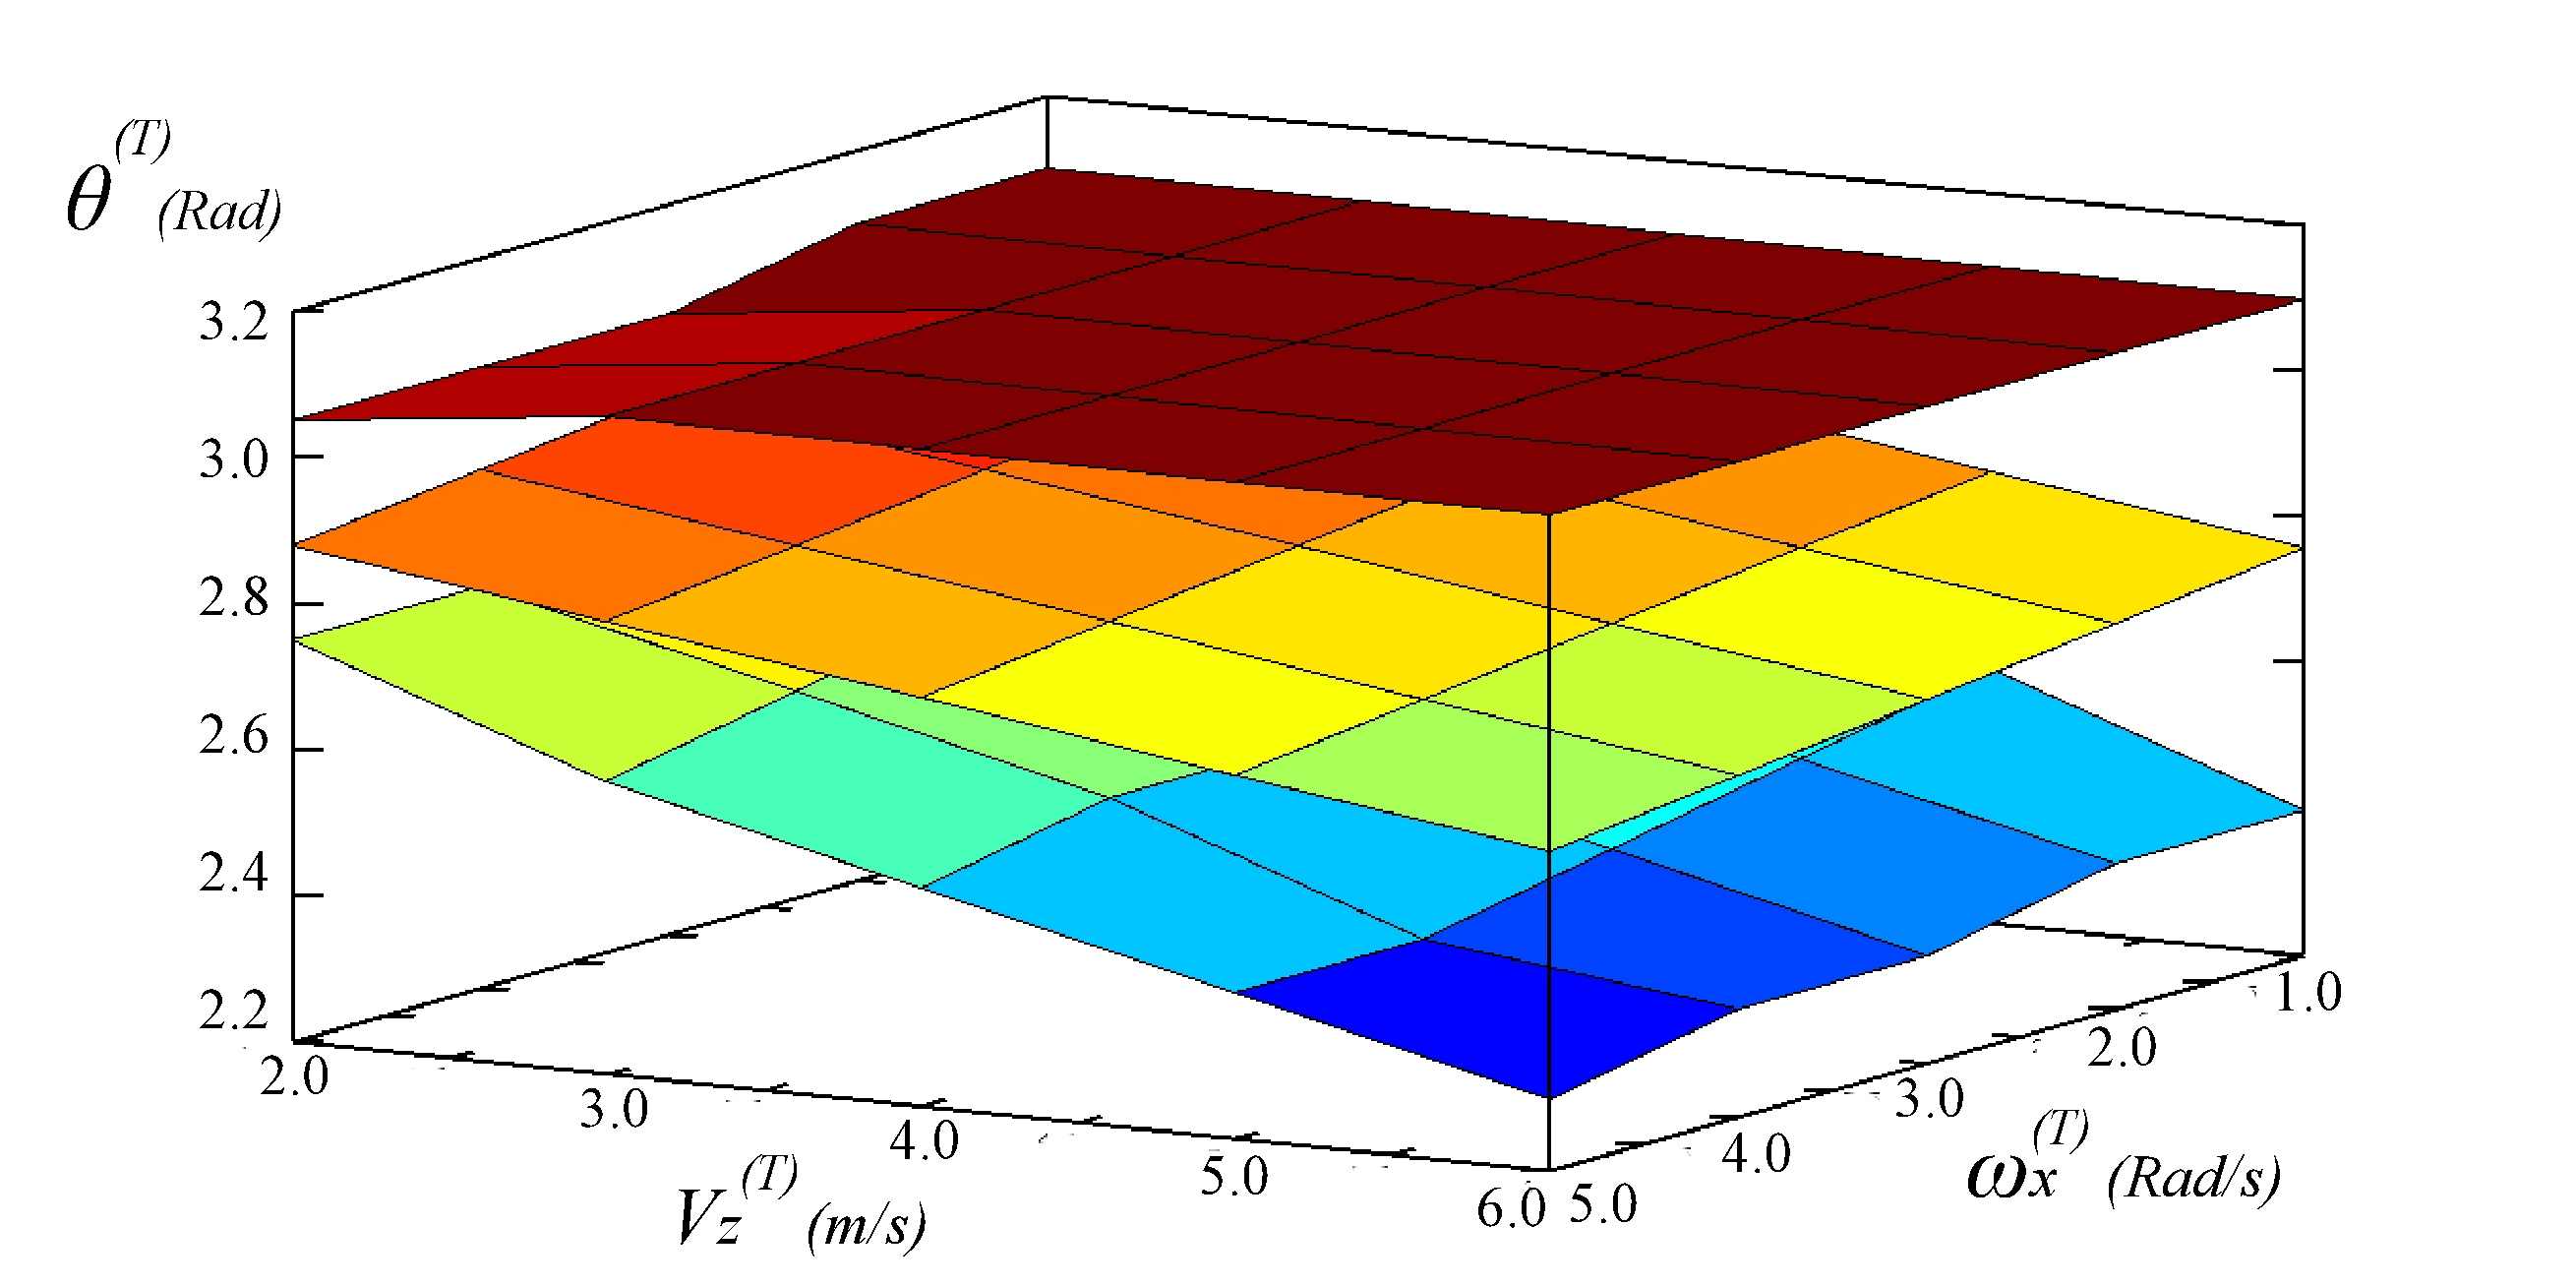
\includegraphics[width=0.49\textwidth]{images/sampleVZWX}
  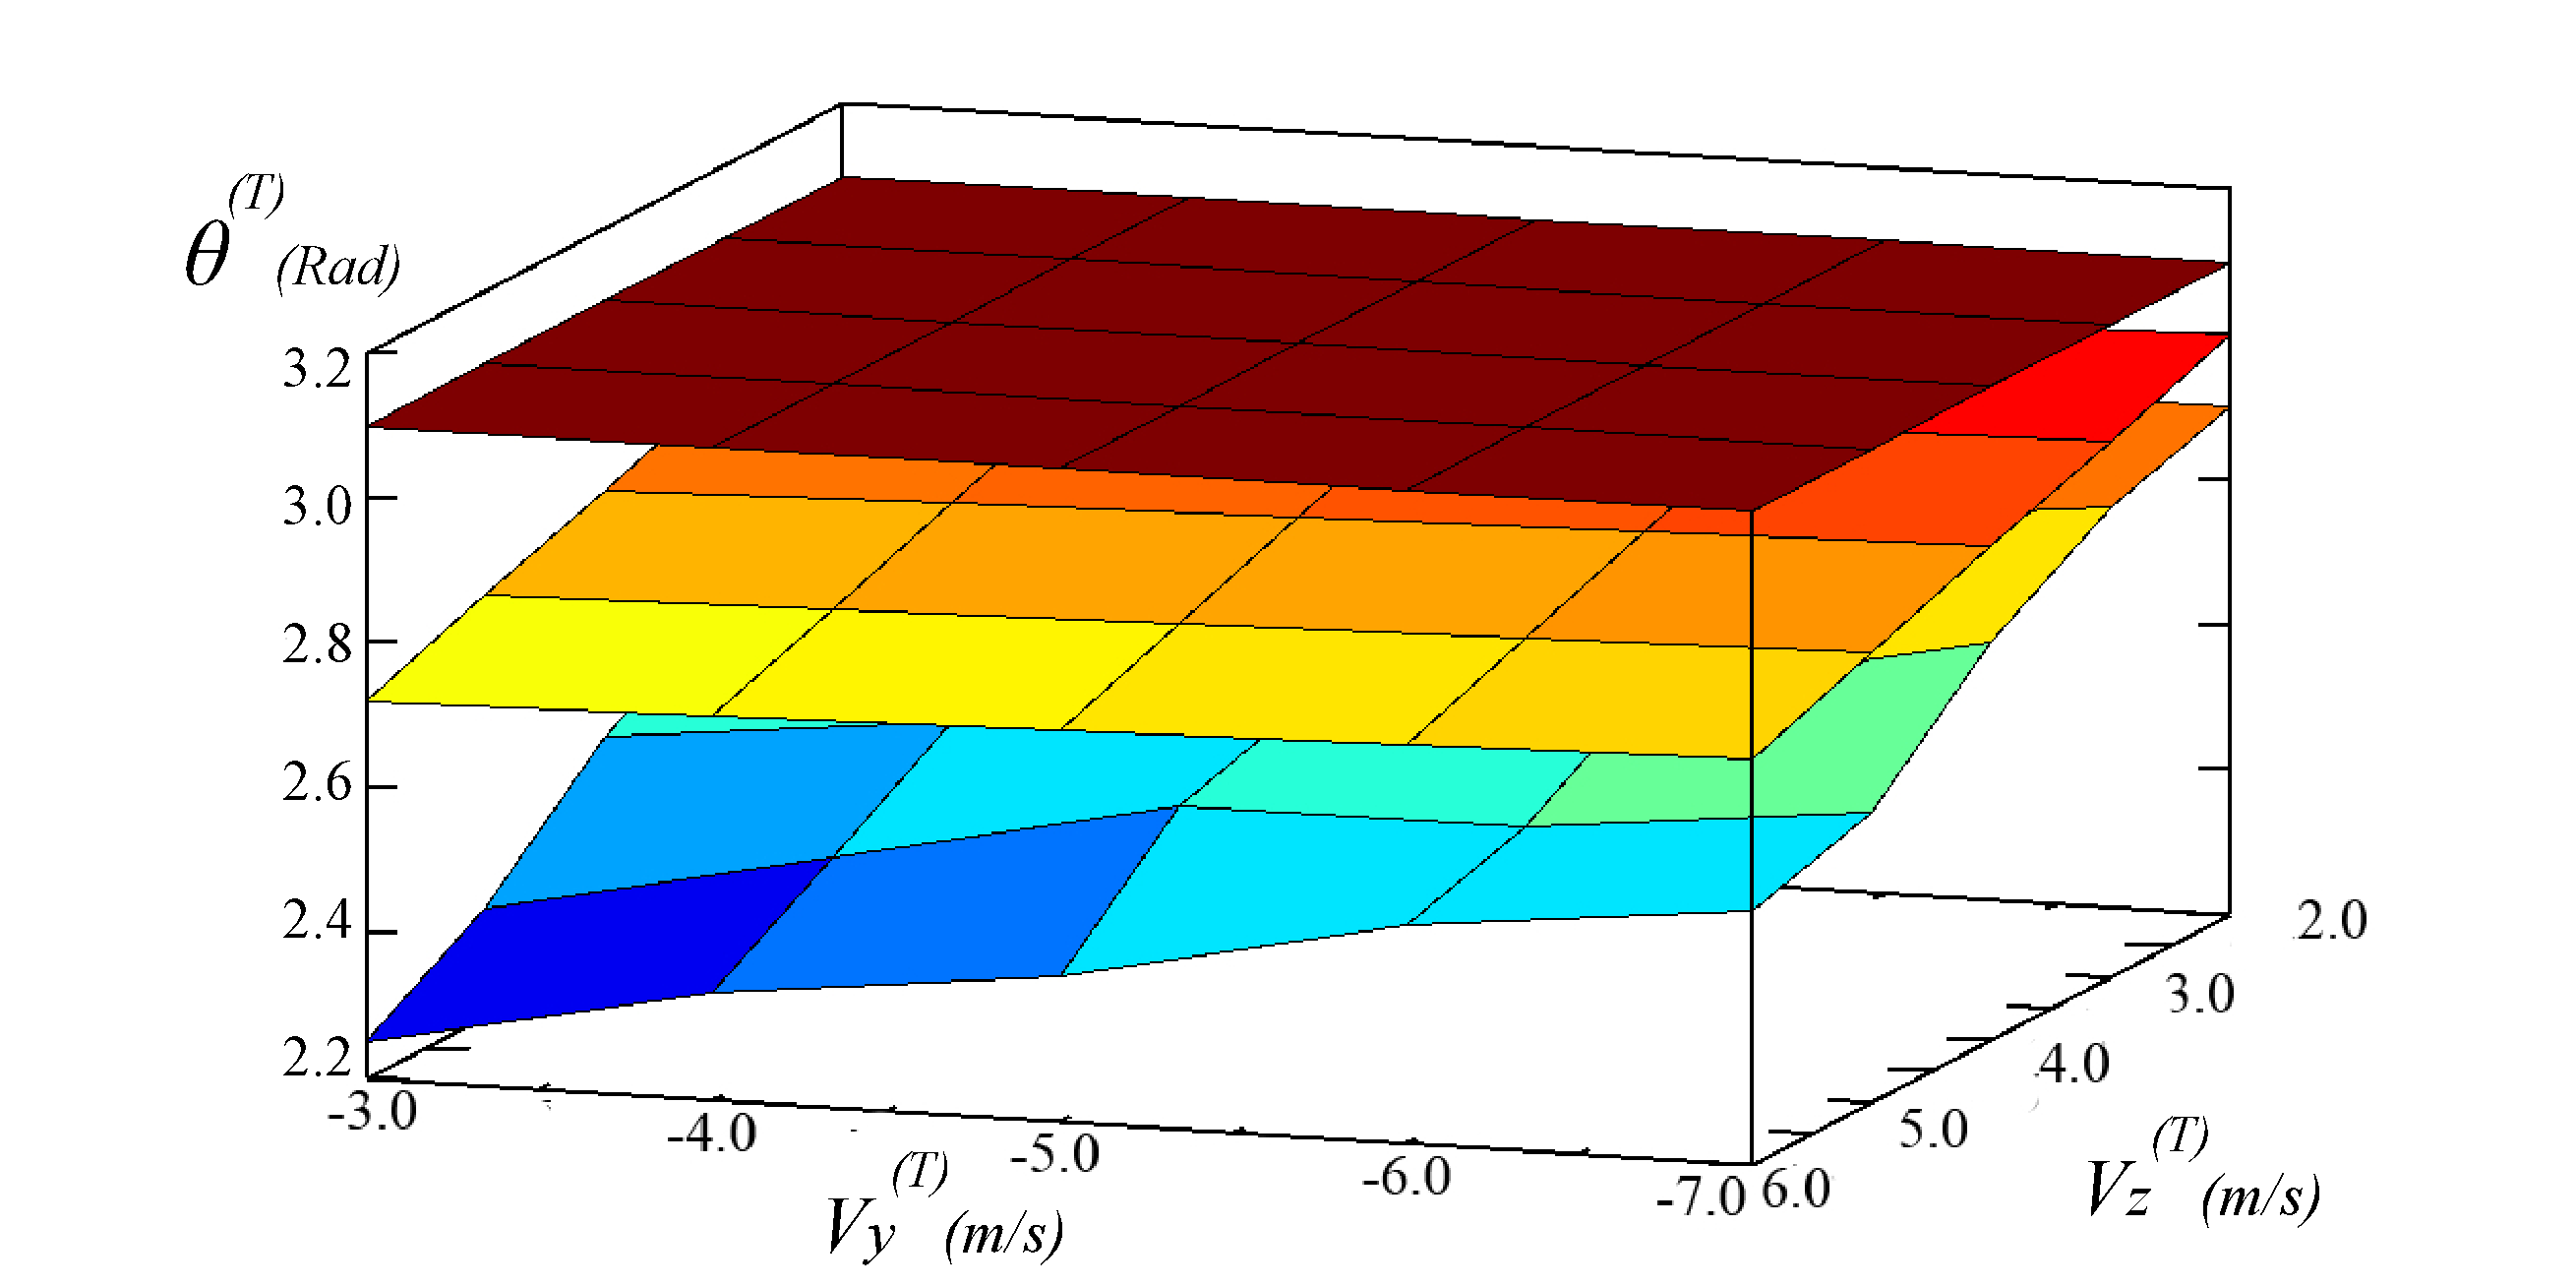
\includegraphics[width=0.49\textwidth]{images/sampleVYVZ}
  \caption{
    Samples for hands-first landing strategy. Successful samples are
    bounded between top and bottom planes along $\theta^{(T)}$
    axis. The middle plane, average of the two, indicates the linear
    relation of the ideal landing condition. 
  }
\ignorethis{
\emph{Top}: x-axis: 
    Domain spanned by $v_z^{(T)}$, $\omega_x^{(T)}$ and $\theta^{(T)}$ \emph{(Top)}
    Domain spanned by $v_z^{(T)}$, $v_y^{(T)}$ and $\theta^{(T)}$ \emph{(Bottom)}
  }
 \label{fig:landing_samplesPlanar}
\end{figure}
 
For the hands-first strategy with planar motion, we consider a
four-dimensional space spanned by $\theta^{(T)}$, $v_y^{(T)}$,
$v_z^{(T)}$ and $\omega_x^{(T)}$. Given a sample in the parameter
space, we run our landing controller to test whether the character can
successfully get up at the end. Empirical results from thousands of
random samples show that the successful region is mostly continuous
and linear (Figure \ref{fig:landing_samplesPlanar}). We can bound the
successful samples in the $\theta^{(T)}$ axis using two hyperplanes.
Taking the average of the maximum and the minimum planes, we derive a
linear relation between the angle of attack and the landing velocities as
\begin{equation}
\label{eqn:landing_approxLandingAngle}
\theta ^{(T)} = a \;v_y^{(T)} + b \;v_z^{(T)} + c \;\omega_x^{(T)} + d
\end{equation}
where $a$, $b$, $c$, and $d$ are the coefficients of the fitted
hyperplane. Note that Equation (\ref{eqn:landing_approxLandingAngle}) is a
sufficient but not necessary condition for successful landing. Most
points between the maximal and minimal hyperplanes also lead to
successful landing motions. This means that even when the character
cannot meet the landing condition exactly, it still has a good chance
to land successfully. For the feet-first strategy, in theory, we need
to consider all six dimensions of linear velocity and angular
velocity. However, our empirical results show that non-planar
velocities do not affect $\theta^{(T)}$ as long as they stay within a
reasonable bound (Figure \ref{fig:landing_sampleNonPlanar}). As a result, the
feet-first strategy is able to handle non-planner falling motion using
the same parameters (but different coefficients) in Equation
(\ref{eqn:landing_approxLandingAngle}).

\begin{figure}[ht]
\center
  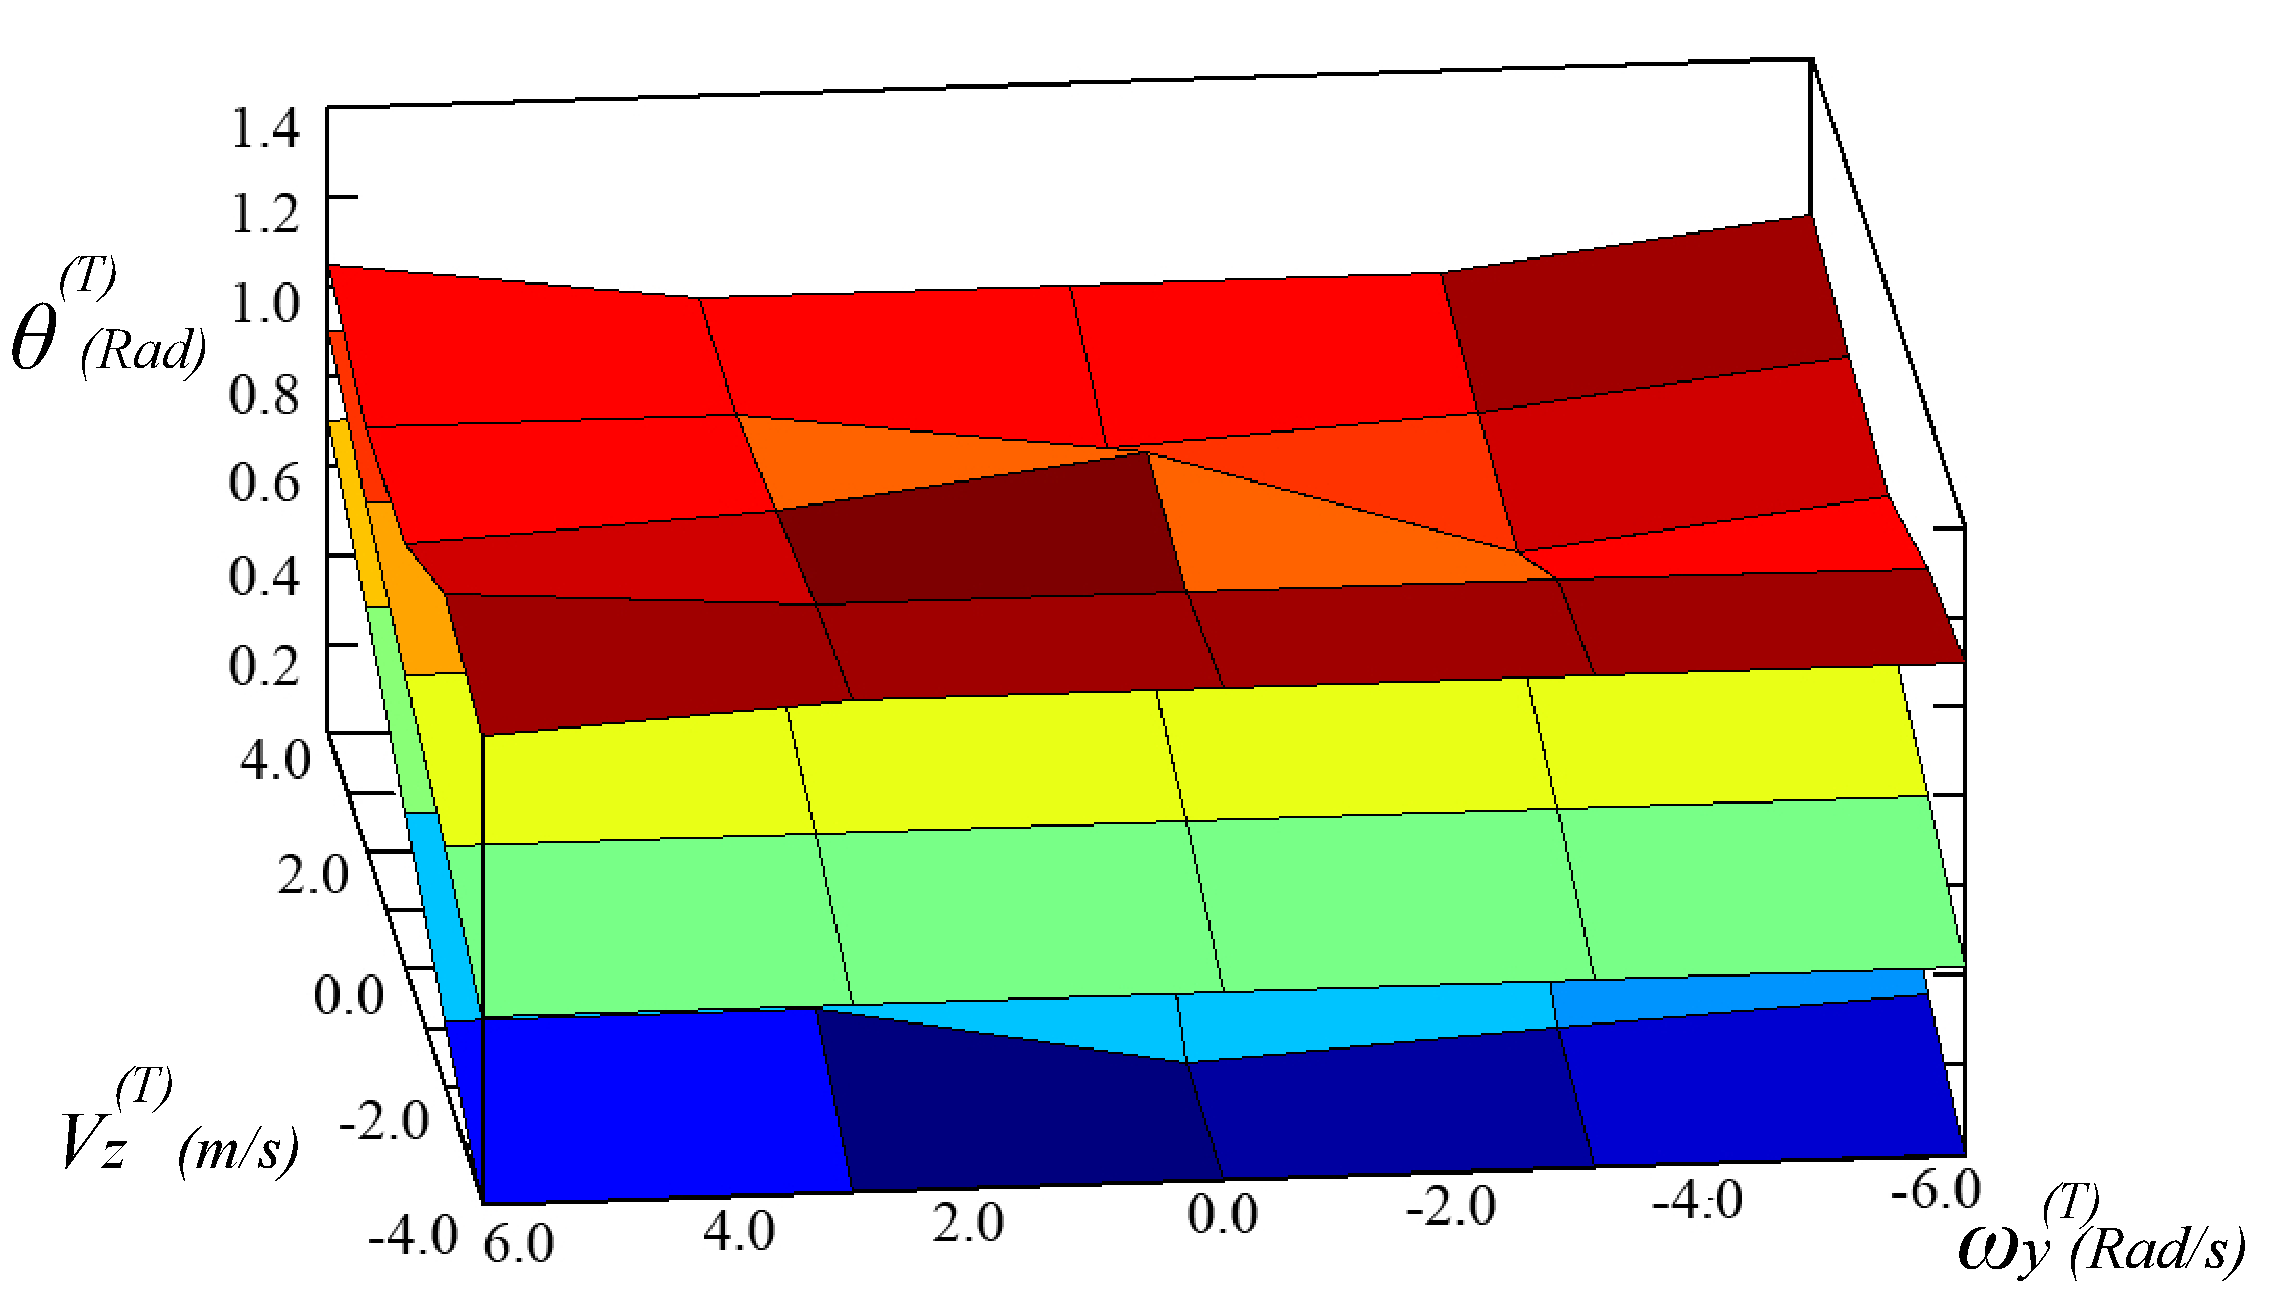
\includegraphics[width=0.51\textwidth]{images/sampleWYflat}
  \caption{
    Samples in the space of $v_z^{(T)}$, $\omega_y^{(T)}$, and
    $\theta^{(T)}$. The spinning velocity $\omega_y^{(T)}$
    has minimal effect on the success of a sample.
  }
 \label{fig:landing_sampleNonPlanar}
\end{figure}


\section{Airborne Phase}
Once the character decides on a landing strategy, the goal of the
airborne phase is to achieve the corresponding landing pose and
landing condition. Because momentum is conserved in air, the linear
velocity, the total airborne time $T$, as well as the angular momentum
are already determined by the initial condition of the fall.  However,
the character can still control the angular velocity $\omega_x^{(T)}$
and the angle of attack $\theta^{(T)}$ by varying its pose (\ie
actuated degrees of freedom (DOFs) excluding the global position and
orientation) to change the moment of inertia. To most effectively
achieve the desired landing condition, we design our airborne
algorithm based on the strategy employed in platform diving
competition, where a highly trained athlete performs a sequence of
predefined poses to manipulate the final orientation and angular
velocity.

To this end, our airborne controller uses a PD servo to track a
sequence of poses that lead to the ideal landing condition. 
The sequence of poses is replanned frequently to correct the errors
caused by perturbation and numerical approximation. Each time the
algorithm makes a new plan, an optimal sequence of poses from the
current moment to the landing moment is computed. This sequence
starts with the current pose $\vc{q}_0$ and ends at the desired
landing pose $\vc{q}_T$ (determined by the landing strategy), with a
duration of $T$ seconds. Our control algorithm searches for an
intermediate pose $\vc{q}^*$ and a duration $\Delta t^*$, such that
the character can reach the ideal landing condition by changing to
$\vc{q}^*$ immediately and holding the pose $\vc{q}^*$ for $\Delta
t^*$ seconds before changing to the final pose $\vc{q}_T$.

We formulate an optimization to solve for an intermediate pose $\vc{q}$
and its holding duration $\Delta t$ that can best achieve the ideal
landing condition. The cost function  $g(\vc{q}, \Delta t)$ is defined
in Equation \ref{eqn:landing_landingCondition}.

\begin{equation}
g(\vc{q}, \Delta t) = \theta^{(T)}(\vc{q}, \Delta t) - a \;v_y^{(T)} - b \;v_z^{(T)} - c\;
\omega_x^{(T)}(\theta^{(T)}) - d
\label{eqn:landing_landingCondition}
\end{equation}
Note that $\omega_x^{(T)}$ is a function of $\theta^{(T)}$ because we
need global orientation of the character at time $T$ to compute the
global angular velocity. If we can compute $\theta^{(T)}$, Equation
(\ref{eqn:landing_landingCondition}) can be readily evaluated. Unfortunately,
for a complex 3D multibody system, an analytical solution for
$\theta^{(T)}$ is not available. We could resort to numerical
simulation of the entire airborne phase, in which the character goes
through $\vc{q}_0$, $\vc{q}^*$, and $\vc{q}_T$ subsequently. However,
involving forward simulation of a full skeleton in the cost function
is too costly for our real-time application.\ignorethis{However, we
  cannot compute $\theta^{(T)}$ analytically and have to resort to
  numerical simulation of the entire airborne phase, in which the
  character goes through $\vc{q}_0$, $\vc{q}$, and $\vc{q}^T$
  subsequently. Such simulation of a full skeleton is too costly for a
  real-time application.} Instead, we simulate a simple proxy model
with only six DOFs. When the character is holding a pose, the proxy
model behaves like a rigid body with a fixed inertia.  When the
character transitions from one pose to another, we assume the inertia
of the proxy model changes linearly within a fixed duration $\Delta
t_C$ ($\Delta t_C = 0.1s$ in our implementation). By simulating the proxy
model for the duration of $T$, we obtain the angle of attack
$\theta^{(T)}$ and angular velocity $\omega^{(T)}$ as
follows.
\begin{eqnarray}
\vc{R}(\theta^{(T)}) = \vc{R}(\theta^{(0)}) + \int_{t=0}^{\Delta t_c}
[\vc{I}^{-1}_{A}(t)\vc{L}]\vc{R}(\theta^{(t)}) dt \nonumber \\ 
+ \int_{t=\Delta t_c}^{\Delta t_c + \Delta
  t}[\vc{I}^{-1}(\vc{q},\theta^{(t)})\vc{L}]\vc{R}(\theta^{(t)}) dt \nonumber \\ + \int_{t=\Delta
  t_c+\Delta t}^{2 \Delta t_c + \Delta t}
[\vc{I}^{-1}_{B}(t)\vc{L}]\vc{R}(\theta^{(t)}) dt \nonumber \\ +
\int_{t=2 \Delta t_c+\Delta t}^T
[\vc{I}^{-1}(\vc{q}_T,\theta^{(t)})\vc{L}]\vc{R}(\theta^{(t)}) dt; \\
\omega^{(T)} = \vc{I}^{-1}(\vc{q}_T,\theta^{(T)})\vc{L}
\end{eqnarray}
where $\vc{R}$ is the rotation matrix, $\vc{I}(\vc{q})$ is an inertia
matrix evaluated at pose $\vc{q}$, and $\vc{L}$ is the angular
momentum. $\vc{I}_{A}(t)$ is an interpolated inertia matrix between $\vc{I}(\vc{q}_0)$ and
$\vc{I}(\vc{q})$, and similarly, $\vc{I}_{B}(t)$ is an interpolated matrix between
$\vc{I}(\vc{q})$ and $\vc{I}(\vc{q}_T)$. The operator $[\;]$ represents the skew
symmetric matrix form of a vector.

% \ignorethis{
% an airborne character can
% only control its pose (\ie actuated degrees of freedom) to change
% the moment of inertia, but cannot directly control the global position and orientation. To this end, we design an airborne controller that
% determines a sequence of poses and uses proportional-derivative (PD)
% servos to track them. In our problem, the initial pose $\vc{q}_0$ is
% determined by the initial conditions of the fall, and the final pose
% $\vc{q}_T$ is determined by the landing strategy. Our algorithm,
% therefore, searches for an intermediate pose $\vc{q}^*$ from a
% predefined pose set and a duration $\Delta t^*$ such that the
% character can achieve the ideal landing condition by changing from
% $\vc{q}_0$ to $\vc{q}^*$ immediately after the fall begins, holding
% $\vc{q}^*$ for $\Delta t^*$ seconds, and changing to $\vc{q}_T$ until
% the end of airborne phase.

% To search for the optimal control parameters, $\vc{q}^*$ and $\Delta
% t^*$, we need to define a cost function, $g(\vc{q}, \Delta t)$ which
% evaluates how well the falling motion achieves the ideal landing
% condition for a given estimate of control parameters. We will first
% describe how we derive landing conditions, followed by the details of
% the search algorithm.


% \paragraph{Search for optimal control parameters.}
% Using the derived landing condition, we now define the cost function
% as

% \begin{equation}
% g(\vc{q}, \Delta t) = \theta^{(T)}(\vc{q}, \Delta t) - a \;v_y^{(T)} - b \;v_z^{(T)} - c\;
% \omega_x^{(T)} - d
% \label{eqn:landingCondition}
% \end{equation}

% Due to conservation of momentum and a known final pose, $v_y^{(T)}$,
% $v_z^{(T)}$ and $\omega_x^{(T)}$ can be computed from the initial
% condition of the fall. The only unknown value in Equation
% \ref{eqn:landingCondition} is $\theta^{(T)}$, which depends on the
% control parameters, $\vc{q}$ and $\Delta t$. Because we cannot compute
% $\theta^{(T)}$ analytically, we propose to simulate the entire
% airborne motion, going through the initial pose $\vc{q}_0$, the
% estimated intermediate pose $\vc{q}$, and the final pose $\vc{q}_T$,
% subsequently.

% However, simulating a full skeleton is too costly for efficient
% evaluation of $g(\vc{q}, \Delta t)$. Instead, we simulate a simple
% model with only six DOFs as a rigid body, but we allow its inertia to
% vary over time. When the character transitions from one pose to
% another, we assume the inertia changes gradually within a fixed
% duration $\Delta t_C$. The angle of attack for the simple model can be
% expressed as following equation and integrated numerically:
% \begin{eqnarray}
% \vc{R}(\theta^{(T)}) = \vc{R}(\theta^{(0)}) + \int_{t=0}^{\Delta t_c}
% [\vc{I}^{-1}(\vc{q}_A(t))\vc{L}]\vc{R}(\theta^{(t)}) \nonumber \\ 
% + \int_{t=\Delta t_c}^{\Delta t_c + \Delta
%   t}[\vc{I}^{-1}(\vc{q})\vc{L}]\vc{R}(\theta^{(t)}) \nonumber \\ + \int_{t=\Delta
%   t_c+\Delta t}^{2 \Delta t_c + \Delta t}
% [\vc{I}^{-1}(\vc{q}_B(t))\vc{L}]\vc{R}(\theta^{(t)}) \nonumber \\ +
% \int_{t=2 \Delta t_c+\Delta t}^T [\vc{I}^{-1}(\vc{q}_T)\vc{L}]\vc{R}(\theta^{(t)})
% \end{eqnarray}
% where $\vc{R}$ is the rotation matrix, $\vc{I}(\vc{q})$ is an inertia
% matrix evaluated at pose $\vc{q}$, and $\vc{L}$ is the angular
% momentum. $\vc{q}_A(t)$ is an interpolated pose between $\vc{q}_0$ and
% $\vc{q}$, and similarly, $\vc{q}_B(t)$ is an interpolated pose between
% $\vc{q}$ and $\vc{q}_T$. The operator $[\vc{a}]$ is the skew symmetric
% matrix of a vector $\vc{a}$.
% }
% \ignorethis{
% To interpolate the inertia, inertia matrices are decomposed into a rotation matrix
%  $\mat{R}$ and a axis-aligned matrix $\mat{I_A}$ using Singular Value Decomposition 
% and interpolated using slerp and weighted sum. 

% \begin{eqnarray}
% \mat{I_0} = \mat{R_0} \mat{I}_{A0} \mat{R_0}^T \nonumber \\
% \mat{I_1} = \mat{R_1} \mat{I}_{A1} \mat{R_1}^T \nonumber \\
% \mat{R}(w) = slerp(\mat{R_0}, \mat{R_1}, w) \nonumber \\
% \mat{I}(w) = \mat{R}(w) (w \mat{I}_{A0} + (1-w)\mat{I}_{A1}) \mat{R}(w)^T \nonumber
% \end{eqnarray}

% While inertia is updated, angular velocity should be updated as well
% to preserve angular momentum. A rigid body simulation is relatively
% inaccurate comparing to the full simulation, but it is enough to
% approximate the landing angle $\theta(T)$ as shown in Figure
% \ref{fig:inertiaTrajectory}. After the simulaton ended, the cost
% functions returns the difference between the current orientation and
% the desired landing angle of attack $\theta(T)$.  
% }

% %% \sehoon{
To formulate an efficient optimization for real-time application, we
represent the domain of intermediate pose as a finite set of candidate
poses, instead of a continuous high-dimensional Euclidean space. This
simplification is justified because a handful of poses is sufficient
to effectively change the moment of inertia of the character. As a
preprocess step, our algorithm automatically selects the candidate set
$\mat{Q}$ from a motion capture sequence in which the subject performs
range-of-motion exercise. The selection procedure begins with a seed
pose $\bar{\vc{q}}_0$ and increments the set by adding a new pose
$\bar{\vc{q}}_{new}$ which maximizes the diversity of inertia
(Equation \ref{eqn:landing_selectingCandidate}). In our experiment, 16 poses
are sufficient to present a variety of moment of inertia
(Figure \ref{fig:landing_candidatePoses}).



% \ignorethis{ The intermediate pose is chosen from a set of predefined
%   poses $\mat{Q}=\{\vc{q}^*_0, \vc{q}^*_1, ... \}$ that can most
%   effectively change each of the six values of the full-body inertia
%   (Figure \ref{fig:candidatePoses}).  We select the set $\mat{Q}$
%   automatically from the captured range of motion.  We start from a
%   selected seed pose $\vc{q}^*_0$ and increment the set by adding a
%   new pose $q^*_{new}$ which maximizes the diversity of inertia
%   (Equation \ref{eqn:selectingCandidate}).  In our experiment, 16
%   poses are compact but sufficient to handle a wide range of initial
%   conditions.}
% %% }

\begin{equation}
\label{eqn:landing_selectingCandidate}
\bar{\vc{q}}_{new} = \argmax_{\vc{q} \in M} (\min_{\bar{\vc{q}}_j \in Q} \| I(\vc{q}) - I(\bar{\vc{q}}_j)\|) \}
\end{equation}
where $M$ contains the poses in the range-of-motion sequence, $Q$
contains the currently selected candidate poses, and $I(\vc{q})$
computes the inertia of pose $\vc{q}$.

%% During the optimization, we loop over each candidate pose in $Q$. For
To find optimal $\vc{q}^*$ and $\Delta t^*$ for each plan, we start from the current pose as $\vc{q}_0$ and loop over each candidate pose in $Q$. For
each candidate pose $\bar{\vc{q}}_i$, we search for the best $\Delta
t$ such that $g(\bar{\vc{q}}_i, \Delta t)$ is minimized. The search can
be done efficiently using one-dimensional Fibonacci algorithm and the
proxy-model simulation. The optimal intermediate pose $\vc{q}^*$ and
its optimal duration $\Delta t^*$ are used for airborne control.

\begin{figure}[ht]
\center
  %% \includegraphics[width=3.2in]{images/AirbornePoses}
  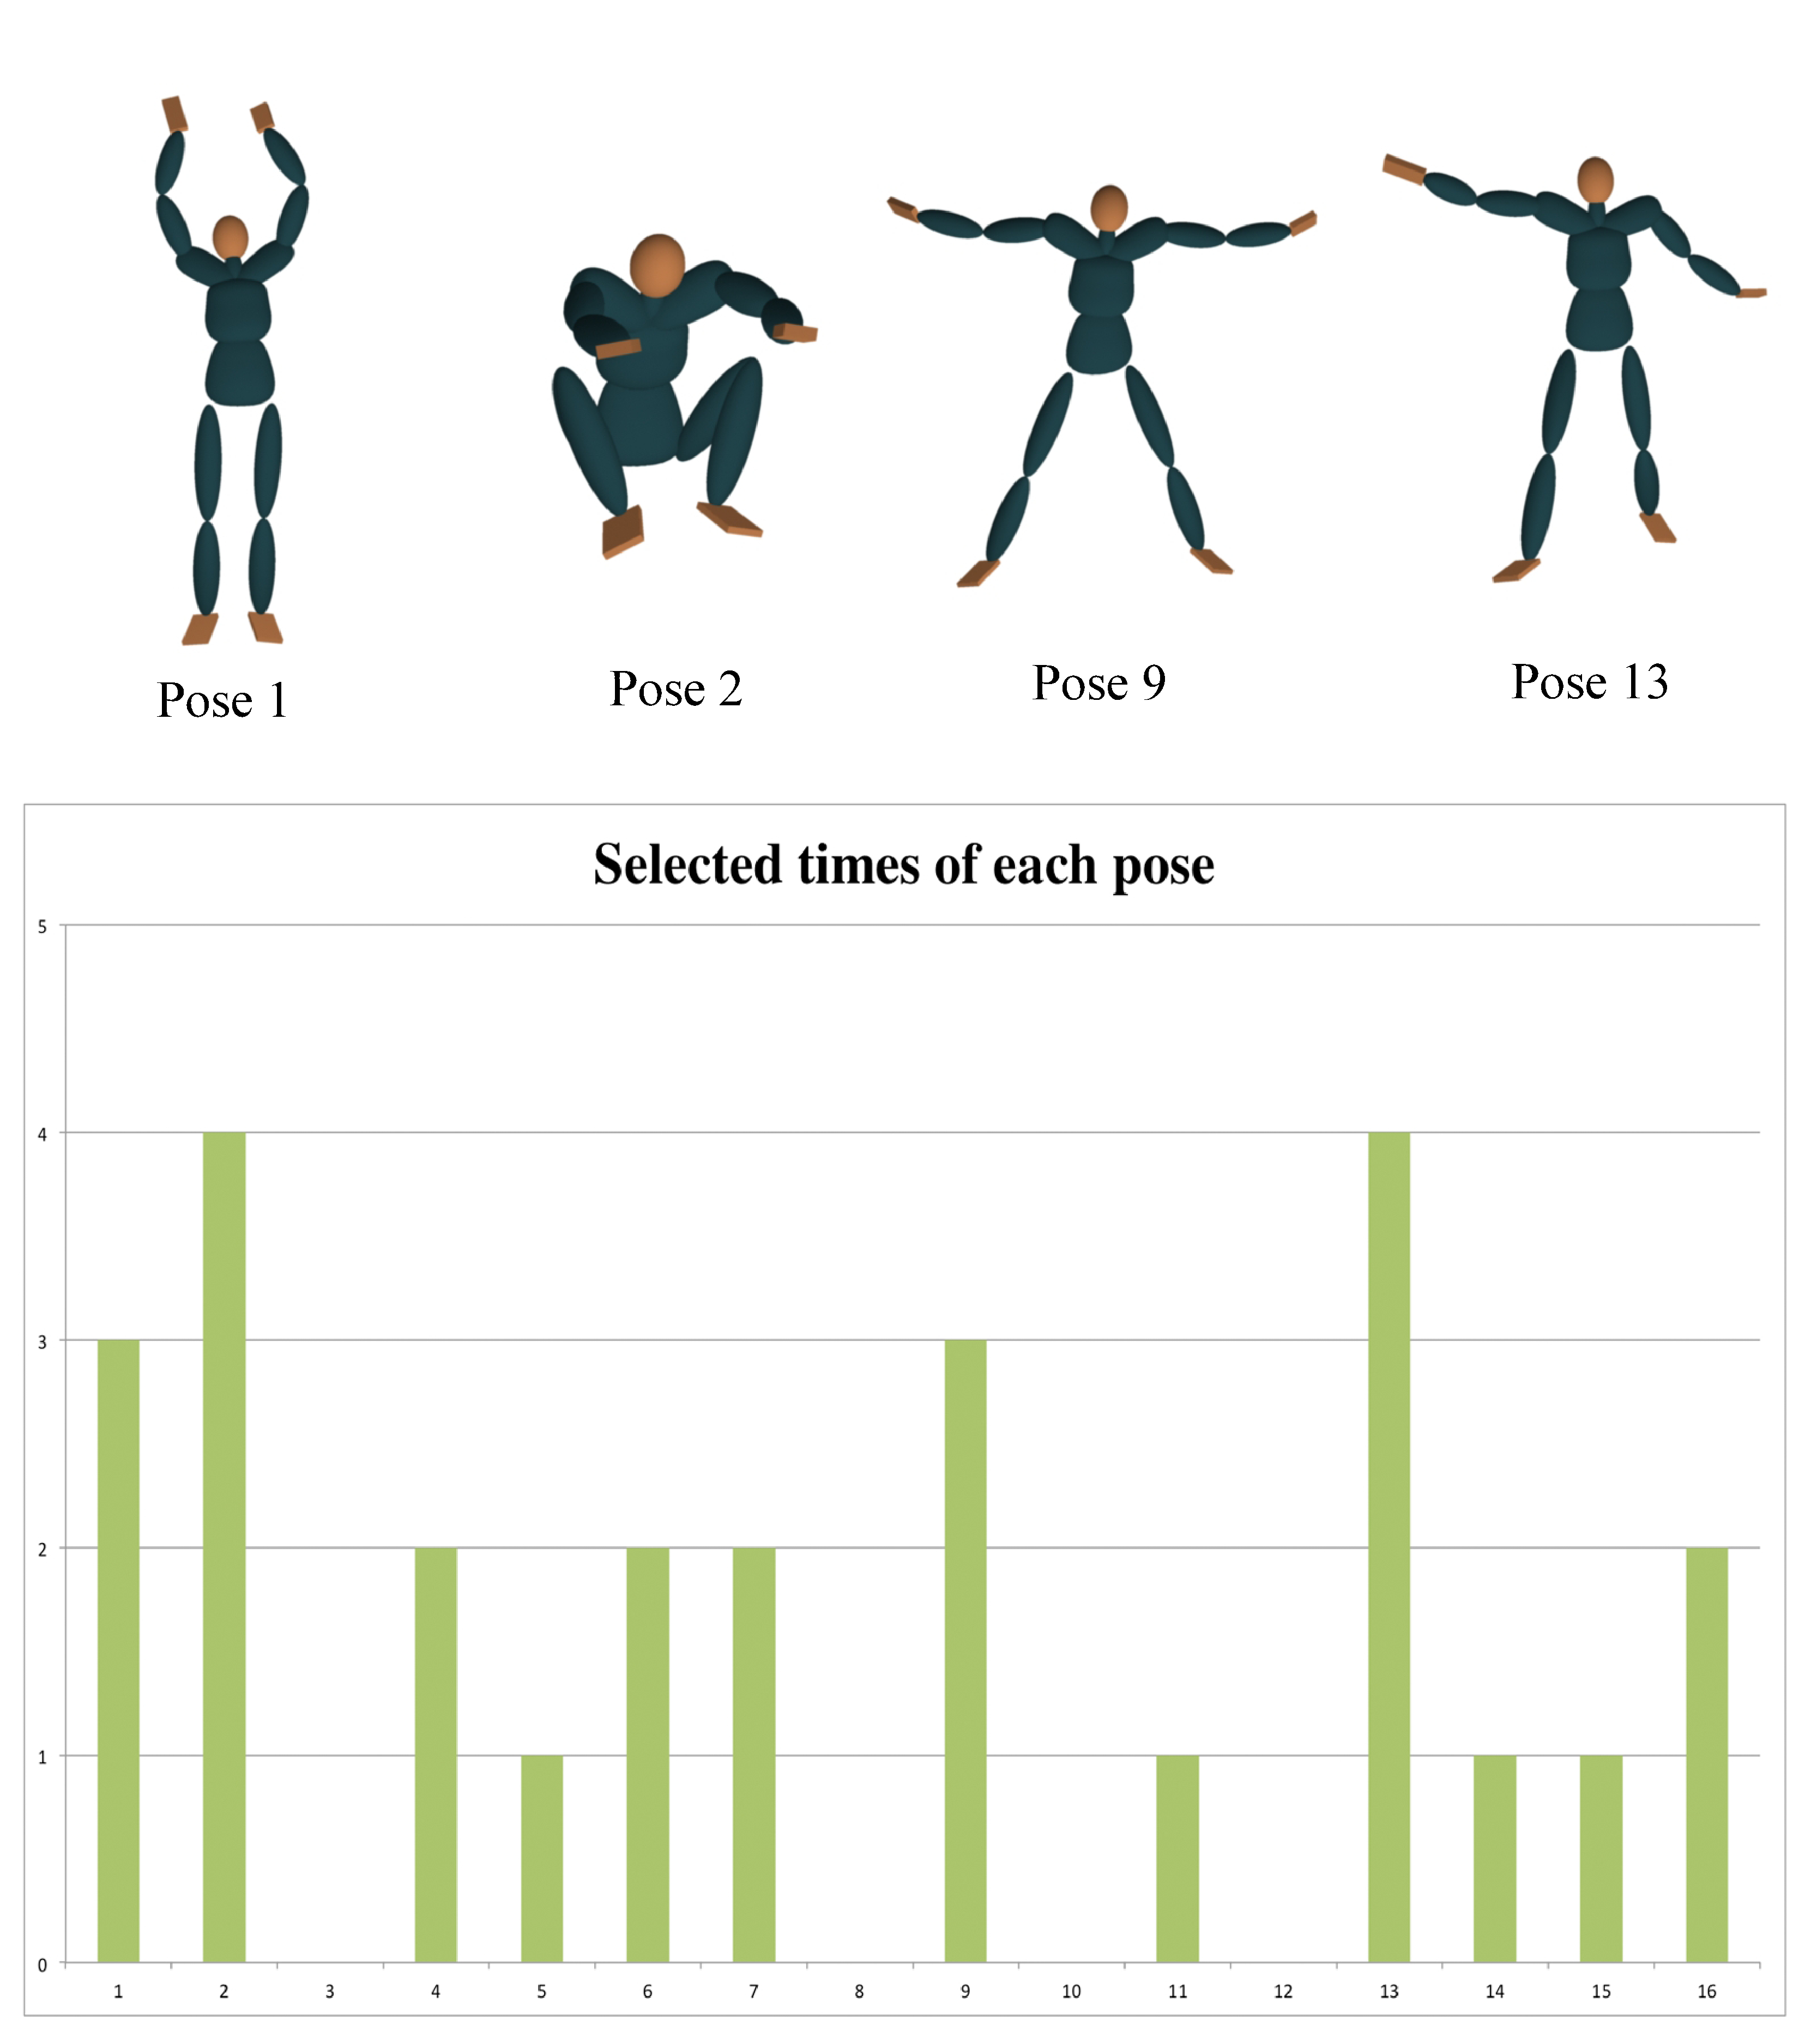
\includegraphics[width=4.2in]{images/PoseWithStats}
  %% \caption{A few popular candidate poses from $\mat{Q}$.
  \caption{
    Among 16 poses in $\mat{Q}$, pose 1, 2, 9, and 13 are frequently 
    selected by the airborne controller
  }
 \label{fig:landing_candidatePoses}
\end{figure}

By design, our algorithm trades off accuracy for efficiency; we use a
fast but less accurate proxy-model simulation and a small set of
predefined poses. Our algorithm is very efficient so that the
character can frequently reassess the situation and replan new poses
to correct any errors or adapt to unexpected perturbations. 

The frequency of replanning can be determined differently for
$\vc{q}^*$ and $\Delta t^*$. In our implementation, we replan
$\vc{q}^*$ at a much lower frequency than $\Delta t^*$ to avoid
unnatural frequent change of poses. In addition, we stop replanning
when the character is within $0.3$ seconds away from the ground.

\section{Landing Phase}
\label{sec:landing_landing}
During landing, the character braces for impact, executes rolling
action, and gets up on its feet. Although these three stages take very
different actions, they share common control goals: modulating the COM
and posing important joints.  We apply the same control mechanism via
\emph{virtual forces} and \emph{PID joint-tracking} to produce the
final control forces for the forward simulator (Figure
\ref{fig:landing_landingOverview}).

\begin{figure}[htbp]
\center
  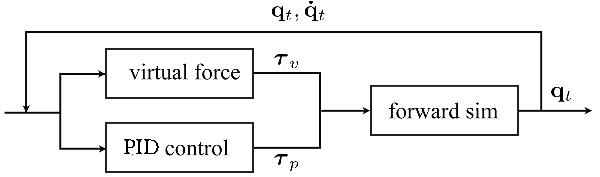
\includegraphics[width=3.2in]{images/landingOverview}
  \caption{Landing phase controller.}
 \label{fig:landing_landingOverview}
\end{figure}

Virtual forces are effective in controlling the motion of the COM. To
achieve a desired acceleration of the COM, $\ddot{\vc{c}}$, we compute
the virtual force as $\vc{f}_v = m \ddot{\vc{c}}$ where $m$ is the mass of the
character. The equivalent joint torque as if applying $\vc{f}_v$ to a
point $\vc{p}$ on the body is $\tau_v = \vc{J}^T (\vc{p}) \vc{f}_v$,
where $\vc{J}(\vc{p})$ is the Jacobian computed at the body point
$\vc{p}$.
If $\vc{p}$ is on a body node in contact with the ground, 
we apply the opposite force ($\vc{f}_v = -m \ddot{\vc{c}}$) in order to
generate a ground reaction force that pushes the COM in the desired direction.
To prevent the character from using excessively large joint
torques, we limit the magnitude of the sum of virtual forces.  A
successful landing motion also requires posing a few important joints
at each of the three stages. We track these partial poses with PID
servos: $\tau_p = k_p (\bar{q} - q) + k_i \int (\bar{q}_t - q_t) dt -
k_v \dot{q}$, where $k_p$, $k_i$ and $k_v$ are the proportional,
integral, and derivative gains respectively, and $\bar{q}$ is the
desired joint angle.  The final control torque is $\tau_v+\tau_p$.
We limit the magnitude of the virtual force to $3000N$ to prevent
excessive usage of joint torques.



\subsection{Impact Stage}
\label{sec:landing_impact}


Impact stage is the most critical stage during landing, which requires
careful control and execution. Human athletes tend to act like a
spring to absorb the effect of impact by flexing their joints between
the points of first contact and the COM. Meanwhile, they also utilize
friction force from the ground contact to adjust forward linear
momentum and angular momentum. Applying these principles, our
algorithm utilizes virtual force technique to achieve contact forces
for desired momentum. In addition, we use joint tracking to provide
sufficient stiffness at contacting limbs and smooth transition to the
next stage. If the character chooses the hands-first strategy, the
final pose at the end of compression can seamlessly connect to the
rolling stage. With the feet-first strategy, an additional
``thrusting'' step is required to transition to the rolling stage. We
define a ``ready-to-roll'' pose that guides the character toward a
rolling motion (Figure \ref{fig:landing_landingPoses}, Right). During this additional
step, the character tracks the ready-to-roll pose while using its feet
to thrust forward after its COM compressed to the lowest point (Figure
\ref{fig:landing_feet-first}).

\begin{figure}[htbp]
\center
%% \begin{minipage}{0.35\textwidth}
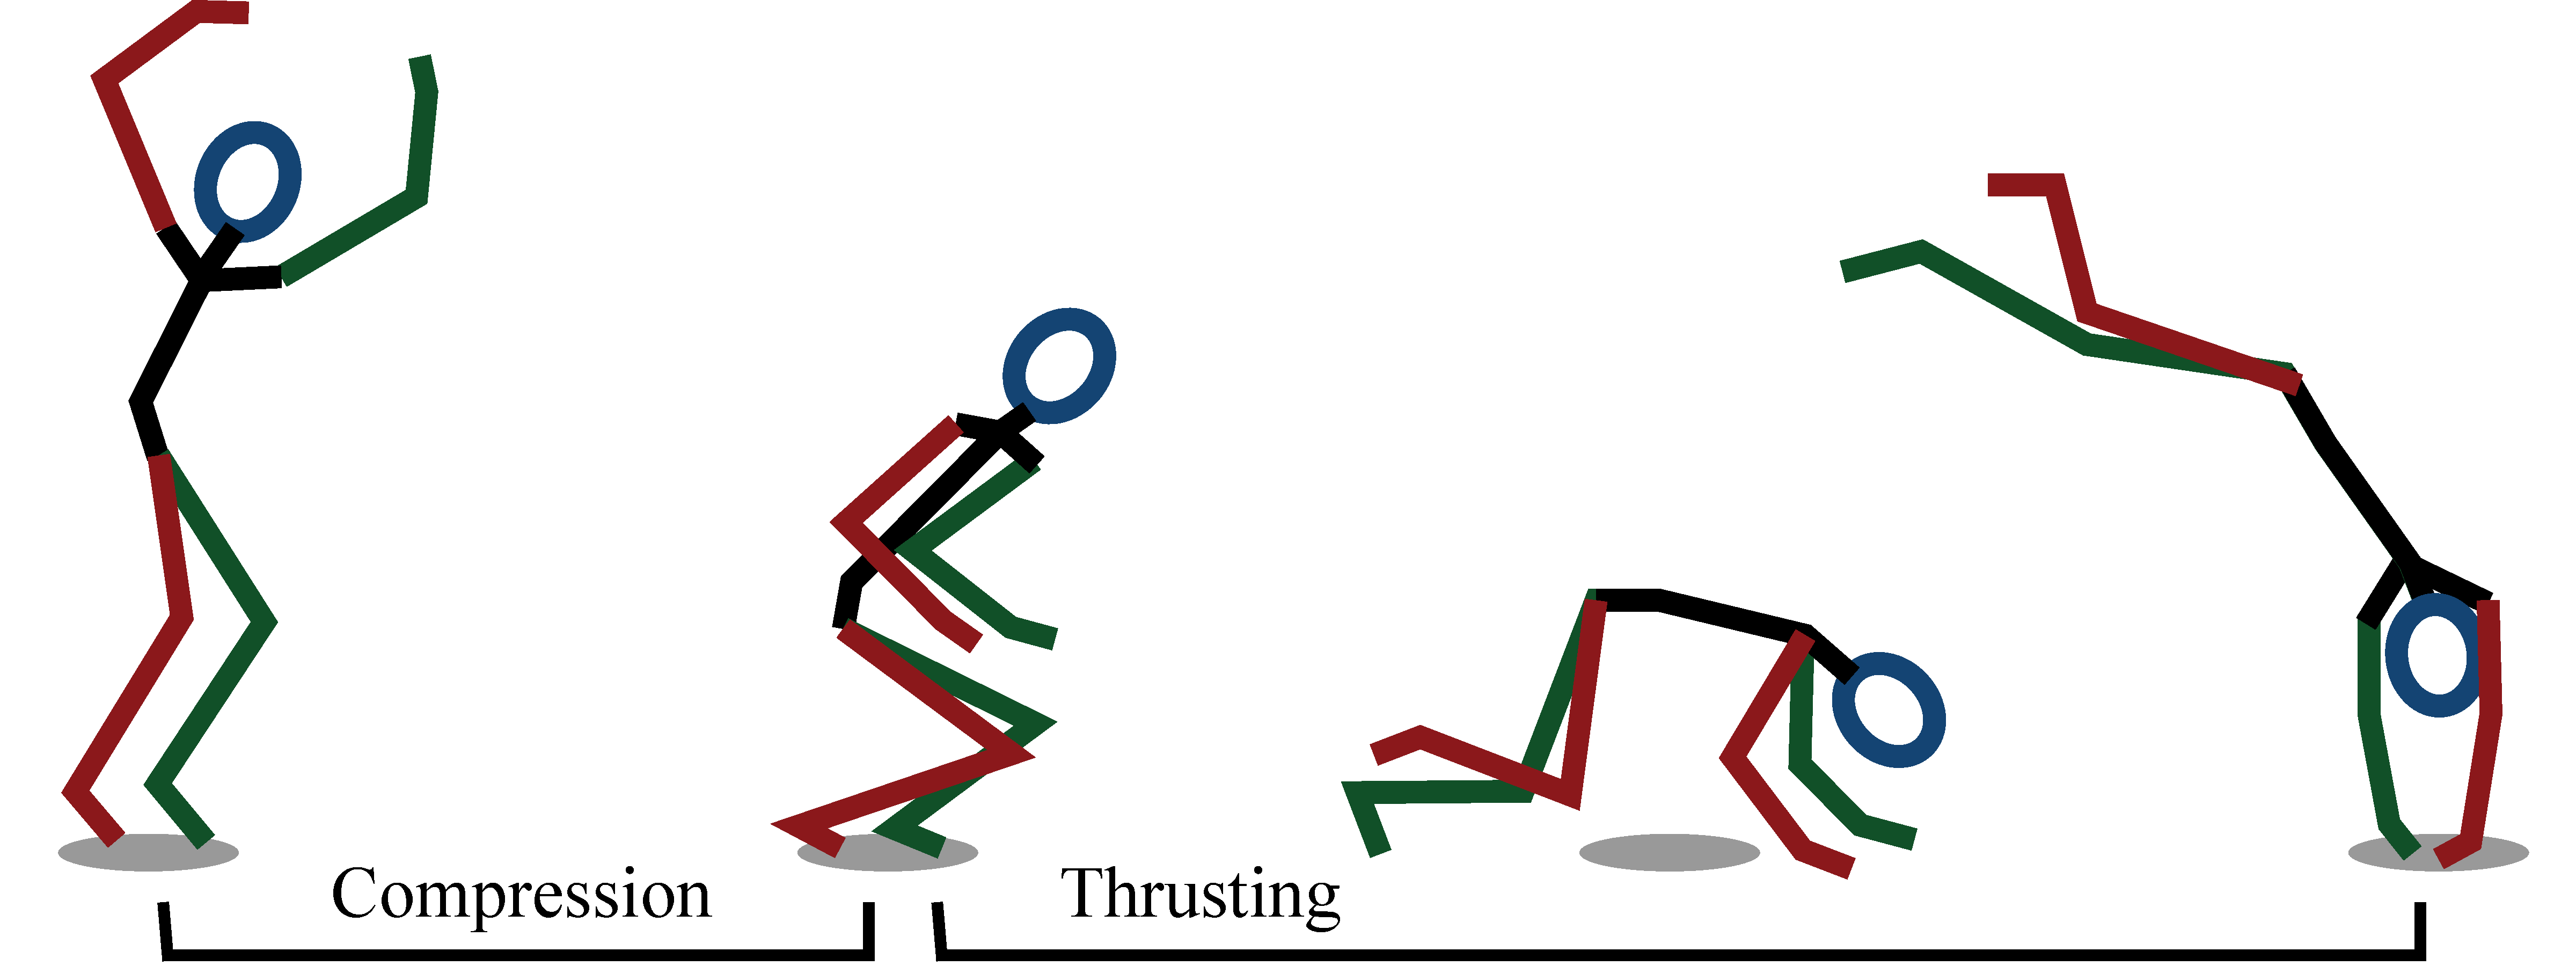
\includegraphics[width=4.2in]{images/feet-first}
\caption{Two-step impact stage for the feet-first strategy.}
\label{fig:landing_feet-first}
%% \end{minipage}
%% \begin{minipage}{0.1\textwidth}
%% 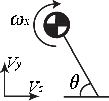
\includegraphics[width=0.8in]{images/COM}
%% \caption{}
%% \label{fig:COM}
%% \end{minipage}
\end{figure}
\ignorethis{
Our algorithm has two different landing styles for impact stage: 
\emph{Landing with hands} and \emph{Landing with feet}. They are not 
only different in the body parts for the first contact but also 
different in the strategies to control the trajectory of COM. While
\emph{Landing with hands} tries to achieve the desired forward momentum
at the lowest point of the COM, \emph{Landing with feet} divides the task
into two stages: compression and thrust. At the compression stages, 
the character acts like a damped spring to absorb all the velocities 
except the forward direction by crouching itself. When the COM reaches 
the bottom point, the algorithm enters the thrust stage and 
commands the character to kick the ground for the desired forward 
linear and angular momentum.}

\textbf{Virtual force.} The most important goal during the impact
stage is to stop the downward momentum before the character tragically
crashes into the ground. We do so by applying virtual forces to
control the vertical position and velocity of the COM. In addition,
our algorithm favors virtual forces that result in temporally smooth
ground reaction forces to distribute the impact evenly over
time. \ignorethis{in hopes of avoiding large joint stress at all
  times.} With these control goals, our algorithm aims to
use constant acceleration of the COM to achieve the desired COM
position $\bar{c}_y$ and velocity $\bar{\dot{c}}_y$ from the current
state ($c_y$ and $\dot{c}_y$).
\begin{equation}
\label{eqn:landing_controlY}
\ddot{c}_y = \frac{1}{2}(\bar{\dot{c}}_y^2 - \dot{c}_y^2) / (\bar{c}_y-c_y)
\end{equation}
A virtual force of $-m\ddot{c}_y$ in the vertical direction is then evenly
distributed to the end-effectors that are in contact with the ground.

Virtual forces in the horizontal direction are important to achieve
the desired forward linear momentum and angular momentum at the end of 
compression, or to achieve the desired forward thrust for the feet-first
strategy. We use a simple feedback mechanism to compute the desired
horizontal acceleration of the COM.
\begin{equation}
\label{eqn:landing_controlXZ}
\ddot{c}_{x/z} = k_v (\bar{\dot{c}}_{x/z} - \dot{c}_{x/z})
\end{equation}
where $\bar{\dot{c}}_{x/z}$ is the desired COM velocity in forward and
lateral directions and $k_v$ is the damping coefficient. The
corresponding virtual force is distributed to the contacting
end-effectors inversely proportional to their distances to the
COM.

\begin{table}
\center
{
%% \small
\caption{Control parameters. 
}


\begin{tabular}{|c |c|c|c|c|c| }
\hline
\label{tab:landing_tracking}

& {\small Hip} & {\small Lower spine } & {\small Upper spine } & {\small Neck } & {\small Knee } \\ \hline 
\textbf{$k_p$} & {\small 90.0} & {\small 300.0}& {\small 180.0}& {\small 10.0} & {\small 60.0} \\ \hline 
\textbf{$k_d$} & {\small 20.0} & {\small 60.0} & {\small 40.0} & {\small  2.0} & {\small 13.0} \\ \hline


& {\small Ankle } & {\small Clavicle } & {\small Shoulder} & {\small Elbow } & {\small Wrist } \\ \hline 
\textbf{$k_p$} & {\small 15.0} & {\small 180.0}& {\small 120.0}& {\small 60.0} & {\small  9.0} \\ \hline
\textbf{$k_d$} & {\small  6.0} & {\small 40.0} & {\small 27.0} & {\small 13.5} & {\small  4.0} \\ \hline

%% \textbf{$k_p$} 
%% & {\tiny 90.0} & {\tiny 300.0}& {\tiny 180.0}& {\tiny 10.0} & {\tiny 60.0} 
%% & {\tiny 15.0} & {\tiny 180.0}& {\tiny 120.0}& {\tiny 60.0} & {\tiny  9.0} \\ \hline

%% \textbf{$k_d$} 
%% & {\tiny 20.0} & {\tiny 60.0} & {\tiny 40.0} & {\tiny  2.0} & {\tiny 13.0} 
%% & {\tiny  6.0} & {\tiny 40.0} & {\tiny 27.0} & {\tiny 13.5} & {\tiny  4.0} \\ \hline
%% \end{tabular}

%% \begin{tabular}{|c|c|c|c|c|c|}
\hline
{\small \textbf{$\bar{c}_y$} } &
{\small \textbf{$\bar{\dot{c}}_y$} } &
{\small \textbf{$\bar{\dot{c}}_{x/z}$} } &
{\small \textbf{$k_v$} } &
{\small \textbf{$k_p$} (Eq \ref{eqn:landing_controlRoll}) } &  
{\small \textbf{$\omega_{MAX}$} } \\ \hline

{\small 0.4m} & {\small 0.0m/s} & {\small 4.0m/s} & {\small 500} & {\small 800} & {\small 3.3 Rad/s} \\ \hline
\end{tabular}
}
\end{table}


\textbf{Joint tracking.} In addition to virtual forces, we use PID
servos to maintain joint angles of the torso and limbs that are not in
contact, while limbs in contact with the ground act like viscous
dampers (PID control with a zero spring coefficient). We also use PID
control to keep the chin tucked to reduce the chance of the head
impacting the ground. Please see Table \ref{tab:landing_tracking} for all the
parameters in our implementation. We set the constant integral gain
$k_i$ of contacting limbs as $50$, and $0$ for all other joints.



\subsection{Rolling Stage}
\label{sec:landing_rolling}
Once the character's COM passes the hand-ground contact area with
sufficient forward linear and angular momentum, rolling becomes a
relatively easy task. As long as the character is holding a pose with
a flexed torso, a reasonable rolling motion will readily carry out. If
the character wishes to land back on its feet and get up after
rolling, it must also maintain forward momentum and lateral balance
during the roll.

\textbf{Virtual force.} To this end, we apply a virtual force to guide
the horizontal position of the COM toward the feet area, while
restricting it above the support polygon formed by contact points. The
virtual force is applied on the character's hands so that it can use
the entire upper body to maintain momentum and
balance. The virtual force produces the desired acceleration of the COM 
computed using a feedback mechanism:
\begin{equation}
\label{eqn:landing_controlRoll}
\ddot{c}_{x/z} = k_p (\bar{c}_{x/z} - c_{x/z})
\end{equation}
where the desired position $\bar{c}$ is set to be the location of the
left foot.

\textbf{Joint tracking.} During rolling, the character tracks a simple
pose to tuck the head, flex the torso, and position the legs
appropriately. We treat legs asymmetrically to both facilitate
momentum control and improve the aesthetics of the motion. When the
character rolls on its back, it brings the left knee closer to the
chest and casually stretches the right leg. This arrangement helps the
character to regulate the angular velocity using the right leg while
getting ready to stand up on its left foot. Based on the forward
angular velocity at the beginning of the rolling stage, we adjust the
desired tracking angles for the right knee as:
\begin{equation}
\label{eqn:landing_controlLeg}
\theta_R = max( (1 - \omega_x / \omega_{MAX}) \pi, 0 )
\end{equation}
\ignorethis{
Our algorithm applies PD control on head,
torso and legs to track some desired joint angles. Head and torso are
bended in forward direction to make the back of the character round
for smooth rolling.  For controlling legs, we assign the different
tasks to left and right legs.  The left leg is always tightly tucked
toward torso and prepared for stand up.  On the other hand, the right
leg is relatively more stretched to regulate the inertia based on the
current angular velocity. For instance, the right leg is tightly
tucked in low speed and fully straightened in the opposite case. The
role of left and right legs can be swapped.
}
\subsection{Getting-Up Stage}
The last stage of landing phase is to stand up using the remaining
forward momentum. When the COM passes the foot contact, the character
will start to elevate its COM to a desired height.

\textbf{Virtual force.} Similar to previous stages, we again apply
virtual forces on the feet and the hands to control the vertical and
the horizontal positions of the COM respectively. We compute $\ddot{c}_y$
using the same formula from \secref{landing_impact} with different desired
height of the COM. For $\ddot{c}_{x/z}$, we use the same formula as
in \secref{landing_rolling}.

\textbf{Joint tracking.} During the getting-up stage, our algorithm
simply tracks the torso and the head to straighten the spine and untuck the chin.

\ignorethis{
\section{Landing Planner}
\label{sec:landingplanner}

\begin{figure}[ht]
\center
  \includegraphics[width=3.2in]{images/abstractmodel}
  \caption{Abstract Model for Landing Motion}
 \label{fig:landing_abstractmodel}
\end{figure}

The goal of landing planner is to guide COM for a smooth transition between 
airborne planner and rolling planner.
To illustrate the character at landing, we construct an abstract model which is 
a single point mass connected to the fixed contact point (Figure \ref{fig:landing_abstractmodel}).
In other words, it is similar to the inverted pendulum model with the varying length rod. 
To prepare rolling, we want to regulate the linear and angular velocity 
when the point mass is vertical to the contact point ($t = T_v$).
Since there are an infinite number of solutions, we assume 
the constant contact force $\vc{\bar{F}}_C$ to distribute the impact over time.

Therefore, our problem is finding the optimal landing orientation $\mat{R}_L$ 
and duration $T_v$ to achieve the desired linear and angular velocity, 
$\bar{\vc{v}}_{v}$ and $\bar{\vc{\omega}}_{v}$.
From the given $\mat{R}_L$ and the length between COM and the desired end-effectors $l_0$, 
we can calculate the position of COM at the landing $\vc{C}(0)$.
In the similar manner, we can obtain $\vc{C}(T_v)$ from the desired key-frame pose.
With the initial and final positions of COM, we can calculate the desired 
contact force $\vc{\bar{F}_C}$ by solving the following equation:

\begin{equation}
\label{eqn:landing_landingcom}
\vc{C}(T_V) = \vc{C}(0) + \vc{v}(0) T_v + \frac{\vc{\bar{F}}_C}{2m}T_v^2
\end{equation}

In fact, equation \ref{eqn:landing_landingcom} gives us the complete trajectory of COM.
Based on this, we can calculate the linear and angular velocity at time $T_v$.

\begin{eqnarray}
\vc{L}(T_v) = \vc{L}(0) + \int^{T_v}_{0} \vc{C}(t) \times \vc{\bar{F}}_C dt \\
\vc{v}(T_v) = \vc{v}(0) + \frac{\vc{\bar{F}}_C}{m}T_v \\
\vc{\omega}(T_v) = \mat{I}(T_v)^{-1} L(T_v)
\end{eqnarray}

We formulate the optimization for $\mat{R}_L$ and $T_v$
to minimize the difference between the velocity at $T_v$ and the desired velocity.

\begin{equation}
(\mat{R}_L^*, T_v^*) = \argmin_{\mat{R}_L, T_v} 
(w_0|\vc{v}(T_v) - \bar{\vc{v}}_{v}| + w_1|\vc{\omega}(T_v) - \bar{\vc{\omega}}_{v}|)
\end{equation}

Since the optimization problem is non-linear and non-differentiable, 
we apply a derivative free optimization algorithm to solve.
}

\section{Results}

\begin{figure}[ht]
\center
  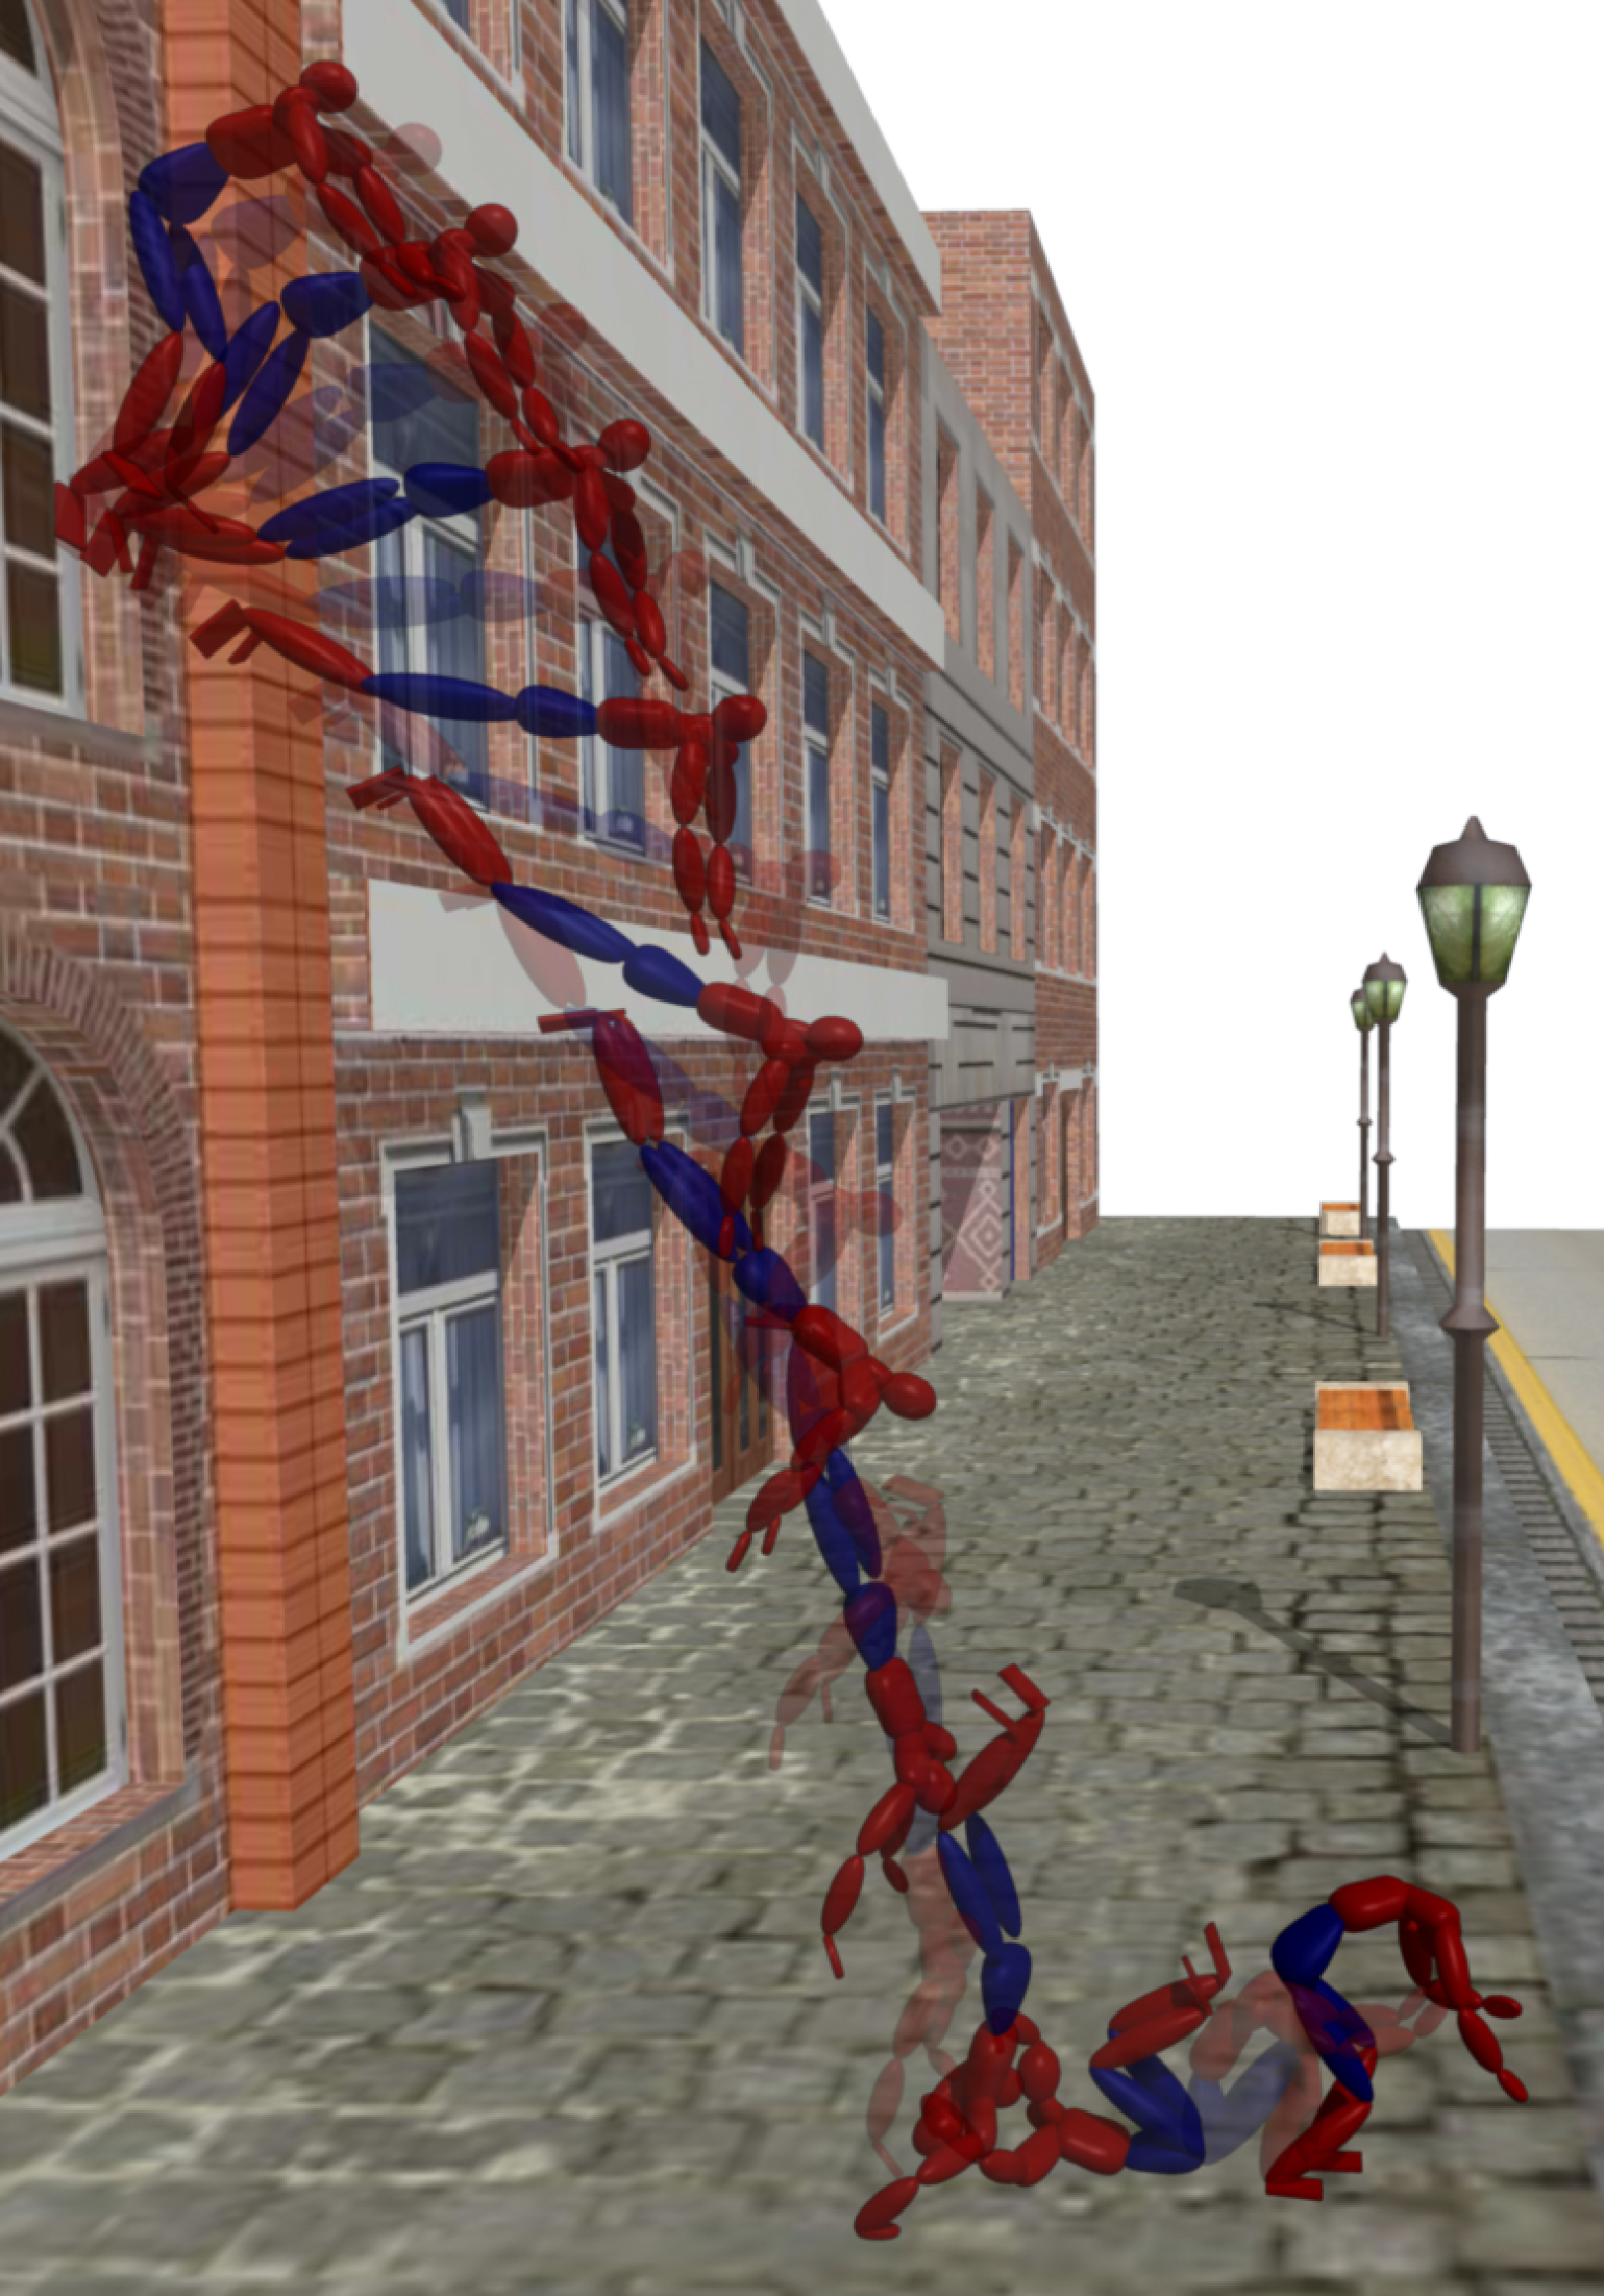
\includegraphics[width=4.0in]{images/ResultImageCol}
  \caption{Hands-first landing motion.}
  \label{fig:landing_resultHands}
\end{figure}

%% \begin{table}
%% \center
%% {
%% %% \small
%% \caption{
%%   Range of initial conditions. Top: Hands-first landing
%%   strategy. Bottom: Feet-first landing strategy.
%%   \sehoon{Statistics for success rate}
%% }
%% \begin{tabular}{|c| c|  c| c|  c| c| c|}
%% \hline
%% \label{tab:initialConditions}
%%   & {\small \textbf{y}}{\tiny(m)} 
%%   & {\small \textbf{$v_z$}}\tiny{(m/s)} 
%%   & {\small\textbf{$v_x$}}{\tiny(m/s)}  
%%   & {\small\textbf{$\omega_x$}}{\tiny(Rad/s)} 
%%   & {\small \textbf{$\omega_y$}}{\tiny(Rad/s)} 
%%   & {\small \textbf{$\omega_z$}}{\tiny(Rad/s)} \\ \hline
%% {\small \textbf{Hands: min}} & {\small 2.0 } & {\small 0.0} & {\small -1.0} & {\small 0.0} & {\small -0.5} & {\small -0.5} \\ \hline
%% {\small \textbf{Hands: max}} & {\small 10.0} & {\small 8.0} & {\small  1.0} & {\small 8.0} & {\small  0.5} & {\small  0.5} \\\hline
%% {\small \textbf{Feet: min}} & {\small 2.0 } & {\small -4.0} & {\small -4.0} & {\small -4.0} & {\small -6.0} & {\small -6.0} \\ \hline
%% {\small \textbf{Feet: max}} & {\small 10.0} & {\small  8.0} & {\small  4.0} & {\small  8.0} & {\small  6.0} & {\small  6.0} \\ \hline
%% \end{tabular}
%% }
%% \end{table}

\begin{table}
\center
{
%% \small
\caption{
  Initial conditions of the examples shown in the video (in order of appearance)
}
\begin{tabular}{| c| c|  c| c|  c| c| c|}

\hline

\multicolumn{7}{|c|}{\small Hands-first landing strategy} \\ \hline

  {\small \textbf{$\vec{C}_y$}}{\tiny(m)} 
  & {\small \textbf{$v_x$}}{\tiny(m/s)}  
  & {\small \textbf{$v_y$}}{\tiny(m/s)}  
  & {\small \textbf{$v_z$}}\tiny{(m/s)} 
  & {\small \textbf{$\omega_x$}}{\tiny(Rad/s)} 
  & {\small \textbf{$\omega_y$}}{\tiny(Rad/s)} 
  & {\small \textbf{$\omega_z$}}{\tiny(Rad/s)} \\ \hline


{\small 10.6} & {\small 0.0} & {\small 0.0} & {\small 4.0} & {\small 8.7} & {\small 0.0} & {\small 0.0} \\ \hline
{\small 5.8} & {\small 0.0} & {\small 0.0} & {\small 2.3} & {\small 5.0} & {\small 0.0} & {\small 0.0} \\ \hline
{\small 10.6} & {\small 0.0} & {\small 0.0} & {\small 6.0} & {\small 2.5} & {\small 0.0} & {\small 0.0} \\ \hline
{\small 2.5} & {\small 0.0} & {\small 0.4} & {\small 8.0} & {\small 5.0} & {\small 0.0} & {\small 0.0} \\ \hline

\hline

\multicolumn{7}{|c|}{\small Feet-first landing strategy}   \\\hline

  {\small \textbf{$\vec{C}_y$}}{\tiny(m)} 
  & {\small \textbf{$v_x$}}{\tiny(m/s)}  
  & {\small \textbf{$v_y$}}{\tiny(m/s)}  
  & {\small \textbf{$v_z$}}\tiny{(m/s)} 
  & {\small \textbf{$\omega_x$}}{\tiny(Rad/s)} 
  & {\small \textbf{$\omega_y$}}{\tiny(Rad/s)} 
  & {\small \textbf{$\omega_z$}}{\tiny(Rad/s)} \\ \hline


{\small 6.0} & {\small 0.0} & {\small 0.0} & {\small 5.0} & {\small 4.0} & {\small -1.0} & {\small -5.8} \\ \hline
{\small 2.7} & {\small 0.0} & {\small -1.0} & {\small 0.0} & {\small 0.0} & {\small 0.0} & {\small 0.0} \\ \hline
{\small 5.5} & {\small 1.0} & {\small 0.0} & {\small 0.0} & {\small 0.0} & {\small 5.0} & {\small 0.0} \\ \hline
{\small 9.6} & {\small -2.0} & {\small 0.0} & {\small -3.5} & {\small 0.9} & {\small 2.1} & {\small -3.9} \\ \hline

\end{tabular}
\label{tab:landing_initialConditions}
}
\end{table}


To evaluate the generality of our algorithm, we simulated landing
motions with a wide range of initial conditions (Table
\ref{tab:landing_initialConditions}), various landing styles (hands-first, feet-first,
consecutive rolls), and different skeleton models. We also demonstrated that
our algorithm is robust to unpredicted runtime perturbations and
different physical properties of the landing surface. Please see the
accompanying video to evaluate the quality of our results.


\paragraph{Feet-first landing strategy.} The most recommended landing
strategy from freerunning community is the feet-first landing. Our
results verify that the feet-first landing strategy is indeed very
robust for falls with arbitrary linear and angular momentum. There are
two key advantages of using feet as the first point of contact. First,
average human has longer and stronger legs than arms. Using legs to
land provides more time and strength to compress and absorb vertical
impact. Second, the feet-first strategy has an additional thrusting
step after compression and before rolling stage. During the thrusting
step, the character can utilize the contact forces to drastically
change the linear and angular velocity in preparation for rolling. Our
results show that a successful forward roll can be carried out even
when the character is falling with backward and lateral linear
velocity or nonplanar angular velocity.
%% (Figure \ref{fig:resultFeet}).

For the feet-first strategy, the coefficients of the landing condition in
Equation (\ref{eqn:landing_approxLandingAngle}) are: $a = -0.01, b = -0.06, c =
-0.03$, and $d = 0.45$. When the character transitions to the rolling
stage, we specified an asymmetric ready-to-roll pose to increase the
visual appeal of the motion.

\paragraph{Hands-first landing strategy.}
Using hands as the first point of contact can generate visually
pleasing stunts (Figure \ref{fig:landing_resultHands}). For falls with
dominant planar velocity ($v_z$ and $\omega_x$), the hands-first
strategy performs as well as the feet-first strategy. However, when
the initial condition has large lateral linear momentum or angular
momentum in yaw and roll axes, the hands-first strategy becomes less
robust. Unlike the feet-first strategy, which has an additional
thrusting step, the hands-first strategy is unable to change forward
direction drastically after landing. This imposes stringent conditions
on the contact forces because, in order to roll successfully, the
contact forces must counteract non-planner momentum, while stopping
downward momentum and maintaining forward momentum. Such forces
usually violate the unilateral constraint of ground reaction force.

For the hands-first strategy, the coefficients of the landing condition
are: $a = -0.01, b = -0.06, c = -0.03$, and $d = 3.08$. Note that the
coefficients are identical to those of the feet-first strategy except
for the constant term, indicating that the gradient of the angle of
attack with respect to the landing velocity is the same between
feet-first and hands-first landing strategies. 
%% We used a symmetric ready-to-roll pose for the hands-first strategy
%% because it reduces the chance of spinning and sideway rolling.

\paragraph{Consecutive rolls.}
Once the character starts rolling, it is rather effortless to continue
on. By looping the end of the rolling stage back to the beginning, we
showed that the character was able to make two consecutive rolls to
break a fall with large forward speed. Falling on multiple surfaces is
also easy to simulate using our controller. One example demonstrated a
continuous sequence of the character landing on the roof of a car,
leaping forward, landing again on the sidewalk, and finishing with a
dive roll (Figure \ref{fig:landing_teaser}). With our controller, a variety of
impressive action sequences can be generated easily without any
recorded or pre-scripted motions.
\begin{figure}[ht]
\center
  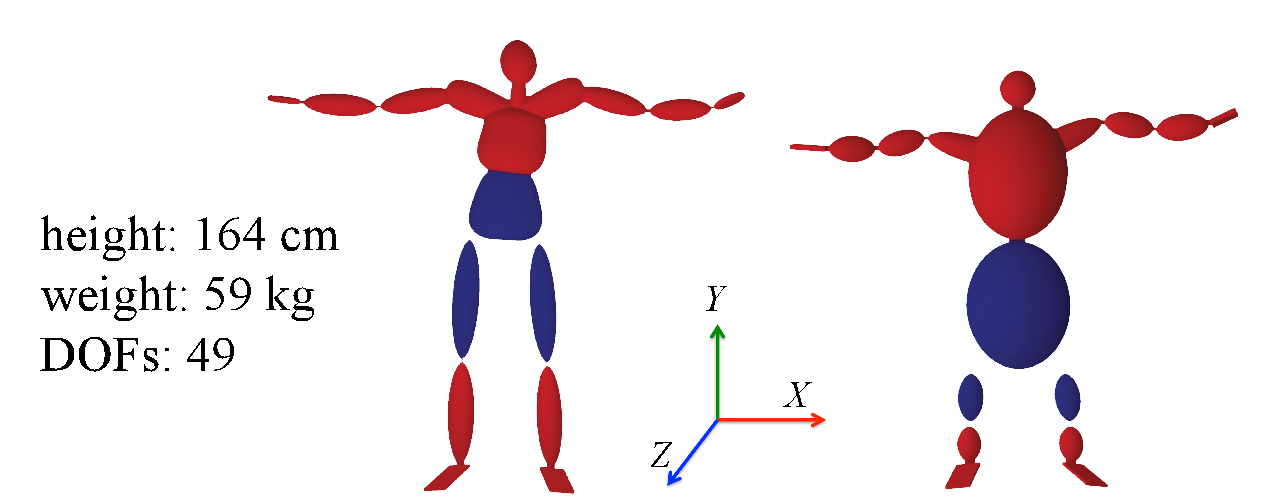
\includegraphics[width=4.2in]{images/diffSkel1}
  \caption{
    Left: The character model used for most examples. Right: A
    character with a disproportionately large torso and short legs.
  }
 \label{fig:landing_models}
\end{figure}
\paragraph{Different skeleton models.}
The character model we used to generate most examples has a height of
$164$cm, a weight of $59$ kg, and $49$ DOFs. The controllers designed
for this character can be applied to a drastically different character
whose torso is twice as long and twice as wide, comparing to the
default character. It also has very short legs and a small head
(Figure \ref{fig:landing_models}). We tested both hands-first and feet-first
landing strategies on this new character. The results are similar in
quality to the default character, although the new character hits its
head on the ground because it is difficult to tuck the head with such
a short neck.
All the control parameters remain the same for the second
character, except for $\bar{c}_y$ increasing by  $5cm$ and the
desired landing angle increasing by $0.25 rad$.


\paragraph{Runtime perturbations.}
One great advantage of physical simulation is that the outcome can be
altered on the fly based on user interactions. We demonstrated the
interactivity of our simulation in two different ways. First, the user
can directly ``drag'' the character to a different location or
orientation when the character is in the air. This example shows off
robustness and efficiency of our airborne controller. As the character
being relocated, it starts to recalculate and finds a new plan to
execute in real-time. Second, we let the user shoot cannons at the
character as a source of external forces. When a cannon hits the
character, it exerts force and torque on the character, causing a
passive response followed by active replanning and execution.

\paragraph{Different landing surfaces.}
We tested our controller on surfaces with different elasticities and
friction coefficients. When the character lands on an elastic surface,
such as a gymnastic floor or a trampoline, the character tumbles in
the air instead of rolling on the ground. We generated a continuous
sequence where the character stopped the fall on an elastic surface by
tumbling three times and finishing with a forward roll. This example
shows that various interesting acrobatic sequences can be
generated by simply concatenating our falling and rolling controllers
repeatedly. In another example, we reduced the friction coefficient to
simulate an icy surface. The character was able to use the same control
algorithm to roll, but failed to stand up at the end.

\subsection{Evaluation}

\paragraph{Performance.}
All the results shown in the video were produced on a single core of
3.20GHz CPU. Our program runs at $550$ frames per second. The
bottleneck of the computation is the optimization routine in the
airborne controller. We use Open Dynamic Engine to simulate the
character. The time step is set at $0.2$ millisecond, and runs
the airborne optimization in 50 Hz.
\begin{figure}[ht]
\center
  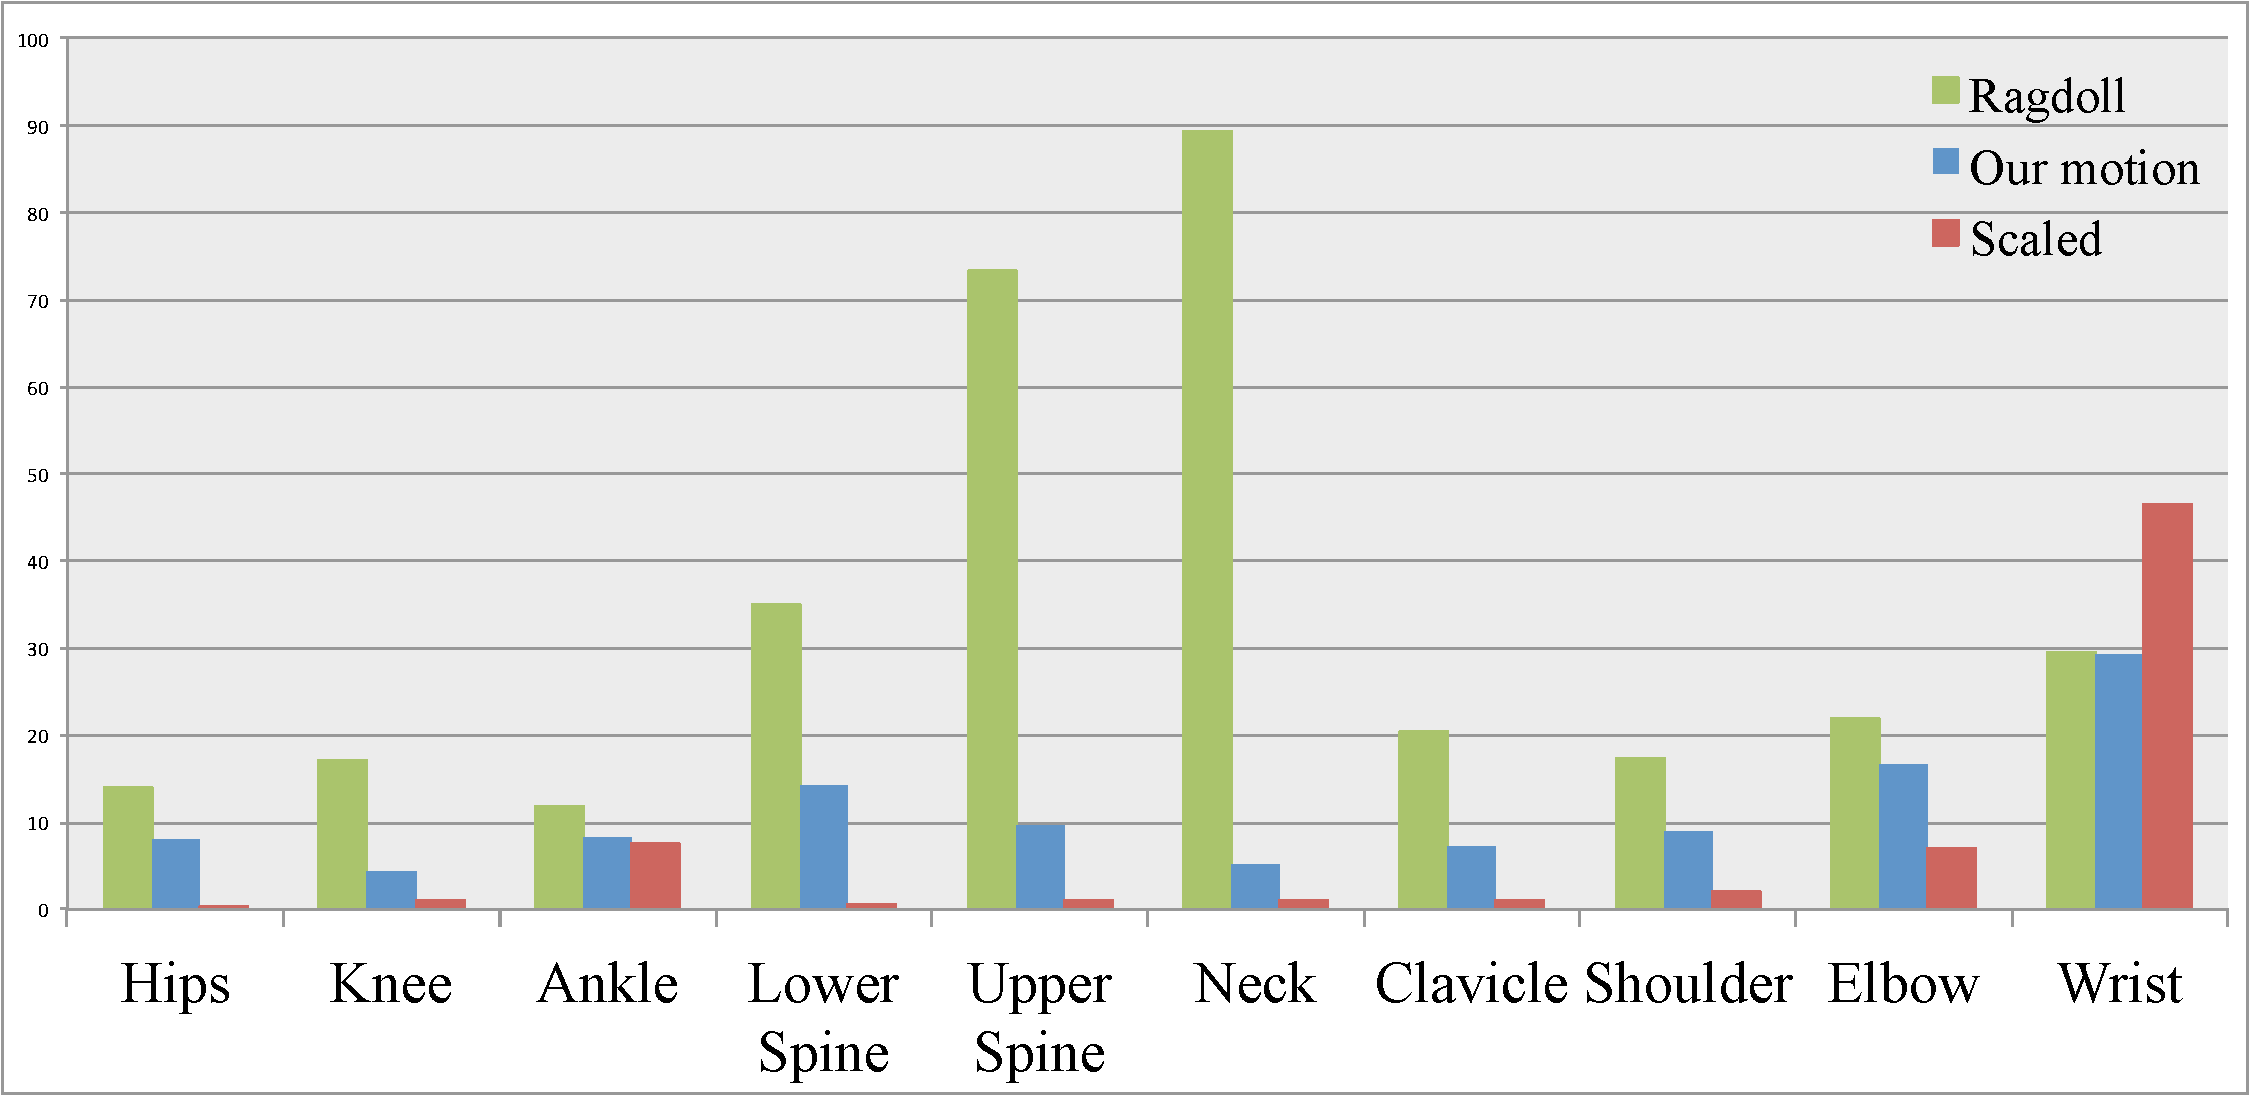
\includegraphics[width=4.2in]{images/stress}
  \caption{
    Maximal stress for each joint from a hands-first landing
    motion. Results are quantitatively similar across all of our
    simulations. Green: Ragdoll motion. Blue: Our motion. Orange: Joint
    stress scaled by mass.}
%% \karen{Order of three bars: Green, blue,
%%       and orange. The joint names from left to right: Hip, Knee,
%%       Ankle, Lower spine, Upper spine, Neck, Clavicle, Shoulder,
%%       Elbow, and Wrist.}
 \label{fig:landing_jointStress}
\end{figure}
\paragraph{Joint stress.}
We approximated joint stress as the constraint force that holds two
rigid bodies together at a joint. For each joint, we computed the
maximal joint stress during the landing phase (Figure
\ref{fig:landing_jointStress}). We observed that, in most trials, the joints
which endure the most impact are those connected to contacting
end-effectors (\ie hands or feet). The spine joints (lumbar and
thoracic vertebrae) and hip joints are also subject to large
impact. However, when we scaled each joint by the total mass it
supports (\eg the hip joint supports the mass of the entire leg), we
found that the joint stress has low variance across the entire
character's body, with the exception of the joints near the
end-effectors.
%% \begin{table}
%% \center
%% {
%% %% \small
%% \caption{Joint Stress Comparison}

%% \begin{tabular}{c  c c}
%% \label{tab:jointStress}
%%  } & \textbf{Ragdoll} & \textbf{Our controller} \\ \hline

%% \textbf{Neck}     & 73.26 &  9.74   \\ \hline
%% \textbf{Spine}    & 35.09 & 14.14   \\ \hline
%% \textbf{Shoulder} & 20.30 &  7.35   \\ \hline
%% \textbf{Hips}     & 13.98 &  7.91   \\ \hline
%% \end{tabular}
%% }
%% \end{table}


When we compared the joint stress between our motion and a passive
ragdoll motion with the same initial condition, the ragdoll motion
caused much more damage on the neck and the spine (Figure
\ref{fig:landing_jointStress}). In fact, the only joints that endured similar
amount of stress were those used for the first point of contact (\eg
wrists or ankles). These results validate that our controller indeed
produces safer landing motion and protects important body parts. We
repeated the experiments for different initial conditions.  In the
worst case of our experiments, the average joint stress is still four
times lower than landing as a passive ragdoll. The data also show that
our controller generates less damaging landing motion even when the
character cannot roll successfully, such as dropping from $20$ meters.


\paragraph{Comparison with video footages.}
We compared our simulated motion side-by-side with a collection of
video footages (\cite{APR:2011:URL}).  The simulations are based on the
same landing strategy and our best guess of the initial conditions from
the videos. Although it is not possible to achieve identical motions,
results show that our motion is qualitatively similar to the video
footages.

\subsection{Limitations}
The main limitation of our work is the lack of balance control after
the character stands up. There are many existing balance control
algorithms we could implement. However, we chose to defer the
implementation until we decide on what the character's next action
should be. In the freerunning scenario, the character transitions to
running motion seamlessly right after a roll. If freerunning is our goal, we
would modify the current get-up control algorithm to provide more
forward thrust. Other possibilities of the next action include
walking, stepping, jumping, or standing still. Different next actions
will result in different balance strategies. Ideally, a character
should be equipped with motor skills to execute all different balance
strategies and autonomously determines which strategy to execute, but
this is considered out of the scope of this work.

Another limitation is the predefined landing pose for each landing
strategy. This inflexibility can negatively affect the character's
ability to adapt to different environments. For example, if the
character lands on a narrow wall, the landing pose needs to be
adjusted on the fly. One possible solution is to use a simple inverse
kinematics method to compute desired joint angles before landing.



\begin{figure}[ht]
\center
  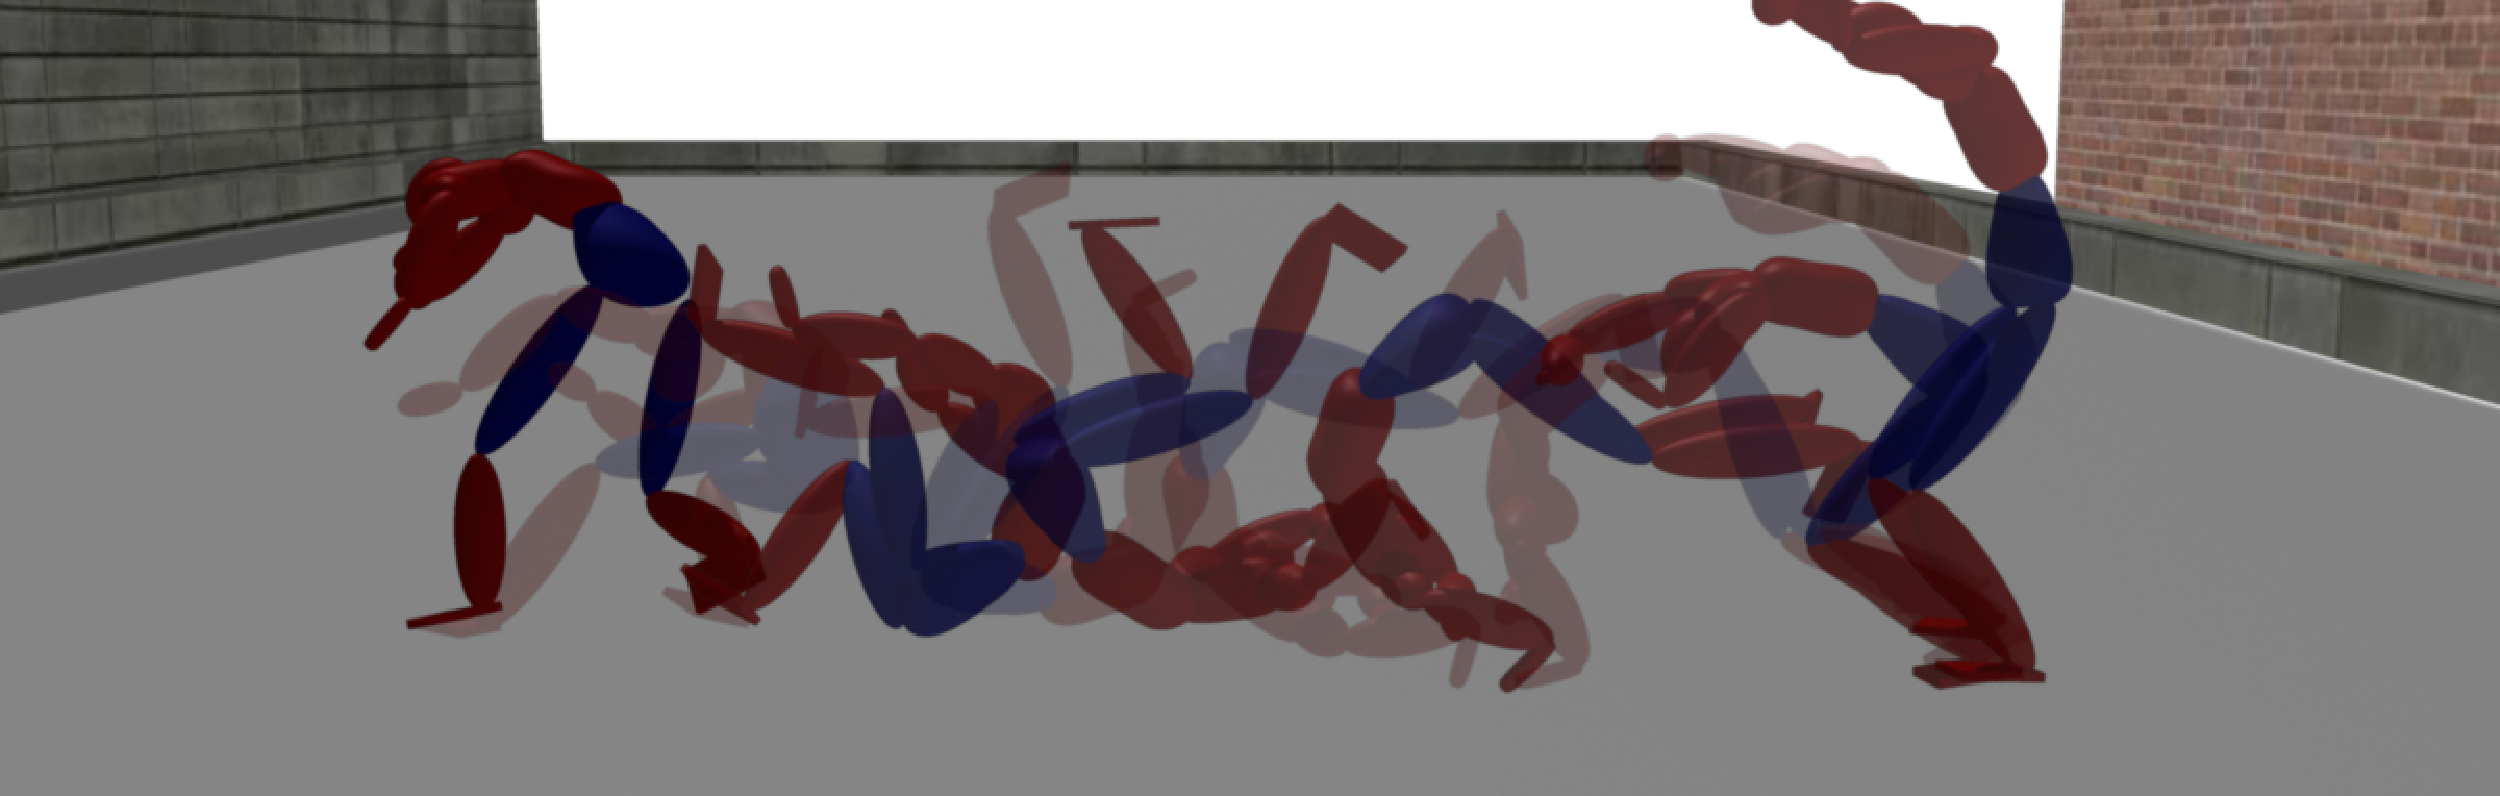
\includegraphics[width=0.95\textwidth]{images/ResultRoll}
  \caption{Feet-first landing motion.}
  \label{fig:landing_resultFeet}

\end{figure}

\section {Discussion}

We introduced a real-time physics-based technique to simulate
strategic falling and landing motions. 
Our control algorithm reduces
joint stress due to landing impact and allows the character to
efficiently recover from the fall.
 Given an arbitrary initial position
and velocity in the air, our control algorithm determines an
appropriate landing strategy and an optimal sequence of actions to
achieve the desired landing velocity and angle of attack. The
character utilizes virtual forces and joint-tracking control
mechanisms during the landing phase to successfully turn a fall into a
roll. We demonstrated that our control algorithm is general,
efficient, and robust by simulating motions from different initial
conditions, characters with different body shapes, different physical
environments, and scenarios with real-time user perturbations.  The
algorithm guides the character to land safely without introducing the
large stress at every joint except for the contacting end-effectors.

Freerunning is a great exemplar to demonstrate human athletic
skills. Those wonderfully simple yet creative movements provide a
rich domain for future research directions. Based on the contribution
of this work, we would like to explore other highly dynamic skills in
freerunning, such as cat crawl, underbar, or turn vault. These motions
are extremely interesting and challenging to simulate because they
involve sophisticated planning and control in both cognitive and motor
control levels, as well as complex interplay between the performer and
the environment.

The landing strategies described in this work are suitable for highly
dynamic activities, but not optimal for low-clearance falls from
standing height. There is a vast body of research work in biomechanics
and kinesiology studying fall mechanics of human from standing
height. One future direction of interest is to integrate this domain
knowledge with physical simulation tools to explore new methods for
fall prevention and protection.



\chapter{Multiple Contact Planning for Humanoid falls}

\graphicspath{{falling/}}

This chapter introduces a new planning algorithm to minimize the damage
of humanoid falls by utilizing multiple contact points. Given an
unstable initial state of the robot, our approach plans for the
optimal sequence of contact points such that the initial momentum is
dissipated with minimal impacts on the robot. Instead of switching
among a collection of individual control strategies, we propose a
general algorithm which plans for appropriate responses to a wide
variety of falls, from a single step to recover a gentle nudge, to a
rolling motion to break a high-speed fall.  Our algorithm transforms
the falling problem into a sequence of inverted pendulum problems and
use dynamic programming to solve the optimization efficiently.  The
planning algorithm is validated in physics simulation and
experimentally tested on a BioloidGP humanoid.

\section{Motivation}
%% \karen{First paragraph: Motivating the importance of fall recovery for
%%   biped humanoids by describing how falls usually happen and what
%%   types of damages they cause. What are the hardware solutions in
%%   practice? Harness? Structural support? What are the drawbacks?}
A humanoid in an interactive environment is often exposed to the
risk of falling due to unexpected contacts or perturbations. A fall
can potentially cause detrimental damage to the robot and enormous
cost to repair. To reduce the likelihood of damaging robots during
online operations, researchers and engineers often cover the robot
exterior with soft guards to absorb the impact of falls
\cite{Missura:2011:DEH,Kobayashi:2011:DHD}. Though practical, these
extra parts can potentially limit the range of motion or change the
contact behaviors.

%% \karen{Second paragraph: An alternative approach inspiring by humans
%%   is for robots to learn basic motor skills to recover from
%%   falls. What are the existing papers in this area? Can be more
%%   thorough since we are not going to have a separate related work
%%   section.}
Alternatively, the robot can learn how to fall safely like humans
do. Fujiware \etal
\cite{Fujiwara:2002:UFM,Fujiwara:2003:FHH,Fujiwara:2004:SKL,Fujiwara:2006:TOF,Fujiwara:2007:OPF}
proposed fall strategies inspired by \emph{Ukemi}, a set of techniques
used in \emph{Judo}.  Ogata \etal \cite{Ogata:2007:FMC,Ogata:2008:RSG}
evaluated the risk of falls using predicted the zero moment point
(ZMP) and optimized the center of mass trajectory to reduce damage.
Ruiz-del-Solar \etal \cite{Ruiz:2009:LTF,Ruiz:2010:FDM} designed
falling sequences for simulated robots playing soccer.
%% Wang \etal \cite{Wang:2012:WTO} formulated an optimization of whole body
%% trajectories as a nonlinear programming problem and solved it with
%% heuristics \karen{this one doesn't say anything.}. 
Wang \etal \cite{Wang:2012:WTO} directly solved joint trajectories
of a three-link robot subject to the full-body dynamics.
Lee and Goswami \cite{Lee:2012:FOB} proposed a control strategy that
reorients the robot to fall on its backpack.
Yun and Goswami \cite{Yun:2014:TFC} described a ``Tripod'' strategy that
utilizes a swing foot and two hands to stop the fall with an
elevated center of mass.  Goswami \etal \cite{Goswami:2014:DCF}
proposed a direction-changing fall control strategy that utilizes
foot placement and inertia shaping to protect both the 
robot and objects/humans in the surroundings.
  
%% \karen{Third paragraph: These existing methods are designed for specific
%%   scenarios. Switching between methods requires an additional decision
%%   maker and carefully designed conditions. We hypothesize that there
%%   exists a continuous space of fall recovery strategies that can be
%%   characterized by the sequence of contact positions and the total
%%   number of contacts. As such, we view existing methods as special cases
%%   in this space. For example, stepping, tripod, Judo, etc...}
These existing methods are effective for specific scenarios in which
the perturbations are assumed within certain range. To select the best
method for the given scenario, an additional decision making process
that classifies initial conditions is required. In this chapter, we
hypothesize that there exists a continuous space of falling strategies
which can be characterized by the sequence of contact positions on the
robot. In this hypothesized space, the existing falling techniques can
be viewed as special cases. For example, the strategy proposed by
Ogata \etal~\cite{Ogata:2007:FMC} employed a single contact at
hands. Fujiwara \etal \cite{Fujiwara:2007:OPF} proposed to use two
contacts, knees and hands, to stop a fall with higher initial
momentum. In \emph{Judo}, multiple contact points from shoulders to
hips are used during a forward roll to break a high-speed fall \cite{ZenpoUkemi:2014:URL}. 

% \updated{These existing methods are designed for specific scenarios including
%   directions and magnitudes of perturbations.
%   Therefore, an additional decision layer that classifies initial conditions
%   is required to select the best strategy for the given scenario.
%   We hypothesize that there exists a continuous space of fall recovery
%   strategies that can be characterized by the sequence of contact positions and
%   the total number of contacts.
%   In this space, we view the existing falling techniques as special cases.
%   For example, the strategy proposed by Ogata \etal~\cite{Ogata:2007:FMC} uses
%   a single contact at hands. 
%   The larger initial momentum requires more contacts, such as knees and hands
%   \cite{Fujiwara:2007:OPF} or a foot and hands \cite{Yun:2014:TFC}.
%   In \emph{Judo}, a forward roll from shoulders to hips is used when being
%   thrown forward \cite{ZenpoUkemi:2014:URL}. } 

  
%% \karen{Fourth paragraph: Based on this hypothesis, we introduce a
%%   general fall recovery control algorithm which unifies all the individual
%%   strategies previously proposed. Details on the key ideas.}
We introduce a general algorithm that unifies the existing techniques
for falling strategies. Our algorithm reacts to a wide range of
initial perturbations by automatically determining the total number of
contacts, the order of contacts, and the position and timing of
contacts. The sequence of contact is optimized such that the initial
momentum is dissipated with minimal damage on the robot. We introduce
an abstract model, which consists of an inverted pendulum and a
telescopic ``stopper'', to approximate the reactive motion when humans
fall. The efficient optimization is achieved by recursive planning in
the space of abstract model using dynamic programming. We demonstrate
that our algorithm plans various falling strategies with different
contact sequences on simulated humanoids and on the actual hardware.

% \updated{Based on the hypothesis, we introduce a general damage reduction
%   algorithm for humanoid falls that provides a unified framework for existing
%   falling strategies. 
%   For the given initial state and possible contacts, our algorithm produces
%   the optimal sequence of contacts and target poses that can break a
%   fall with minimal impulses. 
  %% To make a search in the infinite contact space feasible, our algorithm finds
  %% a sequence in a user-provided contact candidate graph that defines potential
  %% transtions  between contacts, such as ``feet to knees'' or ``hips to hands''.  
  % The efficient optimization is achieved by recursive planning in the space of
  % abstract model using dynamic programming.
  % We demonstrate that our algorithm produces various falling strategies with
  % different contact sequences for a wide range of perturbations.}


\section{The Problem}
Consider a biped humanoid on the ground with an unstable initial state
due to a large initial velocity. If the robot cannot recover its
balance, what is the least damaging way to fall on the ground? It is
well known that the damage incurred at the instance of impact is
mainly due to the sudden change of momentum, which requires a large
impulse applied in a very short period of time. To completely stop a
fall, the robot has no choice but to absorb the initial momentum in
its entirety. However, the change of momentum needs not to happen so
suddenly. With an ideal control policy, the robot should be able to
reduce the magnitude of the impulse at peak by distributing one large
impulse to multiple smaller impulses over multiple contacts with the
ground.

In the discretized time domain, we define the
\emph{instantaneous impulse} at each time step $n$ as 
\begin{equation}
j_n = \int_{hn}^{h(n+1)} f_y(t) dt = h f_y(hn)
\end{equation} 
where $h$ is the
discretized time interval and $f_y(t)$ is the sum of the vertical
contact forces at time $t$. Because the robots considered in this
work are made of hard materials, the contacts between the robot and
the ground can be approximated as collisions between two ideal rigid
bodies. With this assumption, the largest instantaneous impulse during
each contact period typically occurs at the \emph{impact moment}, the
instance when the contact first establishes. The maximum impulse for
the entire falling process can then be defined as
$\max j_n, \; n\in\mathcal{T}$, where $\mathcal{T} = \{\hat{t}^{(i)}
| i = 1 \cdots k\}$. We denote an impact moment for the contact $i$
as $\hat{t}^{(i)}$ and the total number of contacts as $k$. Using this
expression, the goal of our problem is to find a sequence of contact
locations on the robot and their timing, such that $\max j_n$ is
minimized.

\section{The Algorithm}
Our approach to this problem is inspired by the observation on how humans
extend a leg or an arm at the appropriate moment to stop a fall. In
this section, we
will describe an abstract model to approximate this behavior, use this
model to plan the optimal sequence of contacts, and finally execute
the plan on the humanoid robots.

% \updated{Human intentionally reaches the ground to absorb the shock with the
%   desired body parts at the right moments, such as taking a step or pushing
%   the ground with arms.
%   We will describe this behavior with an abstract model and plan the optimal
%   contact sequence using this model.}
%% - Human intentionally establish contacts to break a fall, such as
%% taking a step or stick the arm out.
%% - We seek for an abstract model to represent this behavior and plan
%% the contact sequence using this model.

\subsection{Abstract Model}
\begin{figure}[ht]
\center
  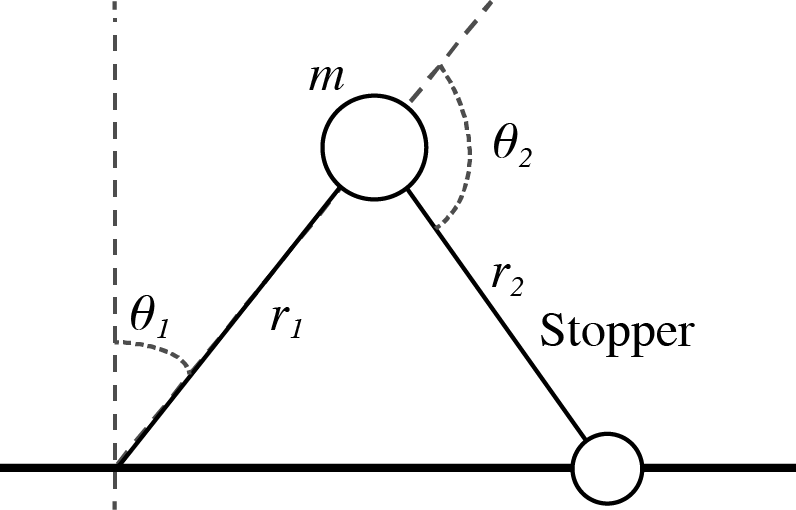
\includegraphics[width=2.5in]{images/tip.png}
  \caption{
    The abstract model consists of a telescopic inverted pendulum and  a massless
      stopper.}
    %% \karen{Replace COM with $m$. Remove the arrow around
    %%   $r_1$. Move ``stopper'' a bit higher as it describes the entire
    %%   stopper not just the tip. Make sure all the math symbols are in
    %%   italic mode to match the format in the text.}
  
  \label{fig:falling_tip}
\end{figure}
The falling motion of biped humanoids has been modelled by a simple 2D
inverted pendulum with a massless telescopic rod
\cite{Fujiwara:2003:FHH,Fujiwara:2006:TOF}. The pivot and the center
of mass (COM) of the pendulum represent the center of pressure (COP)
and the COM of the robot respectively in the sagittal plane. To model
the behavior of breaking a fall using contact, we add an additional
massless telescopic rod, called a stopper, to the standard telescopic
inverted pendulum (\figref{falling_tip}). The configuration of our abstract
model can be defined by the pendulum length ($r_1$), the angle between
the pendulum rod and the vertical line ($\theta_1$), the length of the
stopper ($r_2$), and the angle between the pendulum rod and the
stopper rod ($\theta_2$). We assume that the abstract model has
control over $r_1$, $\theta_2$, $r_2$, but $\theta_1$ is left
unactuated. By controlling these three variables, our goal is to
minimize the vertical impulse at the contact.

Because the stopper is massless, the equations of motion
of the abstract model only depend on $\theta_1$ and $r_1$ and can be
written as:
  \begin{eqnarray}
    r_1 \ddot{\theta}_1 + 2\dot{r}_1\dot{\theta}_1 - g \sin \theta_1
    = 0 
    \label{eq:falling_eom1} \\
    m\ddot{r}_1 - m r_1 \dot{\theta}_1^2 + mg \cos\theta_1 = \tau_{r_1},
    \label{eq:falling_eom2}
  \end{eqnarray}
where $m$ is the mass of the robot and $g$ is the gravitational
constant. The control force $\tau_{r_1}$ is computed based on the
desired velocity of the pendulum rod, $\dot{r}_1^d$:
  \begin{equation}
    \begin{aligned}
      \tau_{r_1}= \frac{m}{h}(\dot{r}_1^d - \dot{r}_1) -
      mr_1 \dot{\theta}_1^2 + mg \cos\theta_1.
    \label{eq:falling_velcon}
    \end{aligned}
  \end{equation}
 %% \karen{assuming $h$ has been defined previously.}

  Though not involved in the equations of motion, the stopper will
  change the momentum of the abstract model whenever it establishes a
  contact with the ground. Let the COM of the pendulum and the tip of
  the stopper be $(x_1, y_1)$ and $(x_2, y_2)$ respectively, with
  respect to the pivot $(0, 0)$.  The momentum due to the vertical
  impulse $j$ generated by the stopper at the contact can be expressed
  as:
  \begin{equation}
    \begin{aligned}
      P_y^+ &= m\dot{y_1}^+ = m\dot{y_1}^- + j \\
      L^+ &=  I\dot{\theta_1}^+ = I\dot{\theta_1}^- - (x_2 - x_1)j,
    \end{aligned}
  \end{equation}
  where $P$ and $L$ are linear and angular momentum of the abstract
  model and $I$ is the estimated inertia. Because we do not know the
  fullbody pose when planning in the space of the abstract model, we
  approximate the inertia using the initial configuration of the robot
  at the beginning of the fall. The superscripts $^-$ and $^+$ denote
  the quantities before and after the impact respectively. For
  inelastic collision, the vertical velocity at the tip of the stopper
  after the impact should be equal to zero, leading to the following
  equation:
  \begin{equation}
    \label{eq:falling_impulse0}
    \begin{aligned}
      0 &= \dot{y}_2^+ = \dot{y}_1^+ - (x_2 - x_1)\dot{\theta}_1^+ \\
      &= (\dot{y}_1^- + \frac{j}{m}) - (x_2 - x_1)(\dot{\theta}_1^- - \frac{(x_2 - x_1)j}{I}) \\
      &= (\frac{1}{m} + \frac{1}{I}(x_2 - x_1)^2) j + \dot{y}_2^-.
    \end{aligned}
  \end{equation}
\eqnref{falling_impulse0} gives a formula to compute the vertical
impulse $j$:
  \begin{equation}
    \begin{aligned}
      j = -\frac{\dot{y}_2^-}{\frac{1}{m} + \frac{1}{I}(x_2 - x_1)^2}.
      \label{eq:falling_impulse1}
    \end{aligned}
  \end{equation}


%%%%%%%%%%%%%%%%%%%%%%%%%%%%%%%%%%%%%%%%%%%%%%%%%%%%%%%%%%%%%%%%%%%%%%%%%%%%%%%%
%%%%%%%%%%%%%%%%%%%%%%%%%%%%%%%%%%%%%%%%%%%%%%%%%%%%%%%%%%%%%%%%%%%%%%%%%%%%%%%%
\subsection{Multiple Contacts}
Multiple abstract models can be strung together to model falling with
a sequence of contacts. Each abstract model describes the motion from
the impact moment $\hat{t}_i$ to the next impact moment
$\hat{t}_{i+1}$. The first abstract model is initialized by the
initial states of COM and COP of the robot at the beginning of the
fall. As the current stopper hits the ground, a new abstract
model is initialized: the COM of the current pendulum at $\hat{t}_{i+1}$ becomes the
initial COM of the new abstract model and the tip of the current
stopper becomes the pivot of the new abstract model. Using multiple
abstract models to represent the falling motion, our goal is to search
for a sequence of contacts whose maximum vertical impulse is
minimized.

Before we formulate the search problem formally, it is important to
note that the number of contacts used to break a fall, in theory, can
be arbitrarily large. In the limit, if a robot could morph into a
rolling ball without slipping, the number of contacts would be infinite and
the vertical impulse of the fall would be zero (the initial momentum is never
dissipated). In practice, however, the robot has only a limited number
of preferred contact points, such as feet, knees, or
hands. Furthermore, these contact points can only be applied in
certain sequences due to the hardware design and kinematic
constraints. 

\begin{figure}[h]
\center
  %% 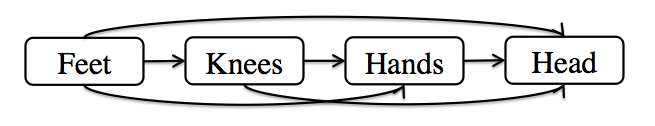
\includegraphics[width=3.0in]{images/contact_graph.png}
  %% 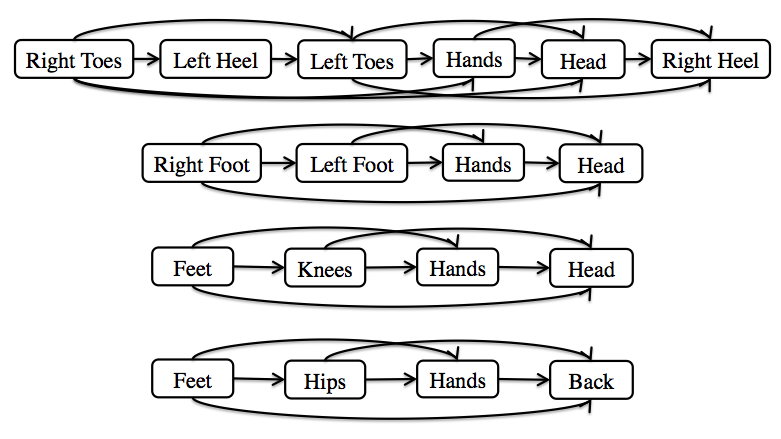
\includegraphics[width=3.0in]{images/four_contact_graphs.png}
  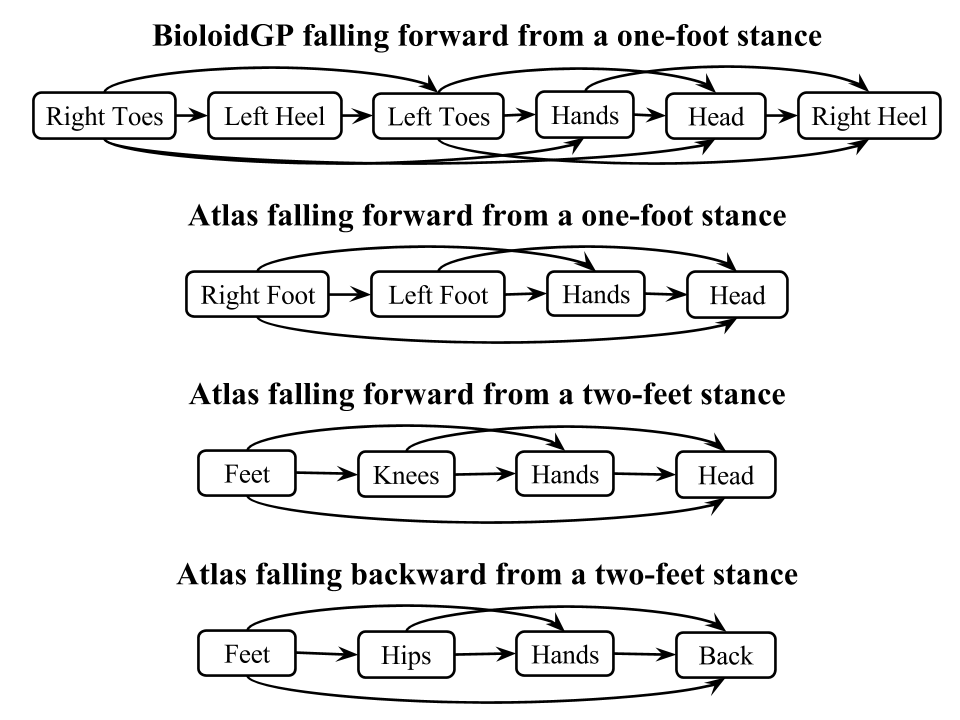
\includegraphics[width=3.1in]{images/all_contact_graphs.png}
  \caption{Contact graphs}
  \label{fig:falling_contact_graph}
\end{figure}

Utilizing these constraints, we introduce a data structure, called a
\emph{contact graph}, to narrow down the search space to only those
contact sequences achievable by a given robot. A contact graph is a
directed graph $G(V_{c}, E_{c})$ which vertices are the preferred
contact points on the robot. If there exists an edge from node $c_1$
to node $c_2$, it indicates that $c_2$ is a valid subsequent contact
point to $c_1$. Given a robot, we can design a contact graph to
represent all possible falling strategies the robot can employ. For
example, a path from feet to knees to hands in \figref{falling_contact_graph}
represents the falling strategy described in \cite{Fujiwara:2002:UFM}.

%%%%%%%%%%%%%%%%%%%%%%%%%%%%%%%%%%%%%%%%%%%%%%%%%%%%%%%%%%%%%%%%%%%%%%%%%%%%%%%%
\paragraph{Plan for contact sequence}
With the contact graph and the initial state of the robot as input, we
now describe our algorithm that searches for an optimal sequence of
contacts using multiple abstract models. 

We formulate the problem as a Markov Decision Process, a framework for
modeling decision making with a long-term cost. We define a state at
each impact moment as
$\vc{x} = \{c_1, \hat{t},\theta_1, r_1, \dot{\theta}_1, \dot{r}_1\}
\in \mathcal{X}$,
where $c_1$ denotes the contact point on the robot, $\hat{t}$ denotes
the time when the impact occurs, and other parameters describe the
position and the velocity of the pendulum at the impact moment. An
action
$\vc{a}=\{c_2, \theta_2, \Delta t, \dot{r}^d_1\} \in \mathcal{A}$
describes the contact point on the robot used as the stopper ($c_2$),
the position of the stopper at the next impact moment ($\theta_2$),
the elapse time from the previous impact moment to the next impact
moment ($\Delta t$), and the desired speed of the pendulum length
during the current contact ($\dot{r}^d_1$). Note that the length of
the stopper $r_2$ at the next impact moment can be derived from $r_1$,
$\theta_1$, and $\theta_2$ by calculating the intersection of the
stopper and the ground.

% The action space is
% defined as $\vc{a}=\{c_2, \dot{r}^d_1, \theta_2, t\} \in \mathcal{A}$
% which comprises the contact point used as the tip of the stopper
% $c_2$, the desired rod velocity $\dot{r}^d_1$, the angle between the
% pendulum rod and the stopper rod $\theta_2$ when it hits the ground,
% and the time $t$ when the stopper hits the ground. Note that the length
% of the stopper $r_2$ at the activation time can be reconstructed from
% $r_1$, $\theta_1$, and $\theta_2$ by calculating the intersection of
% the stopper and the ground.

%% \begin{figure}[ht]
%%   \center
%%   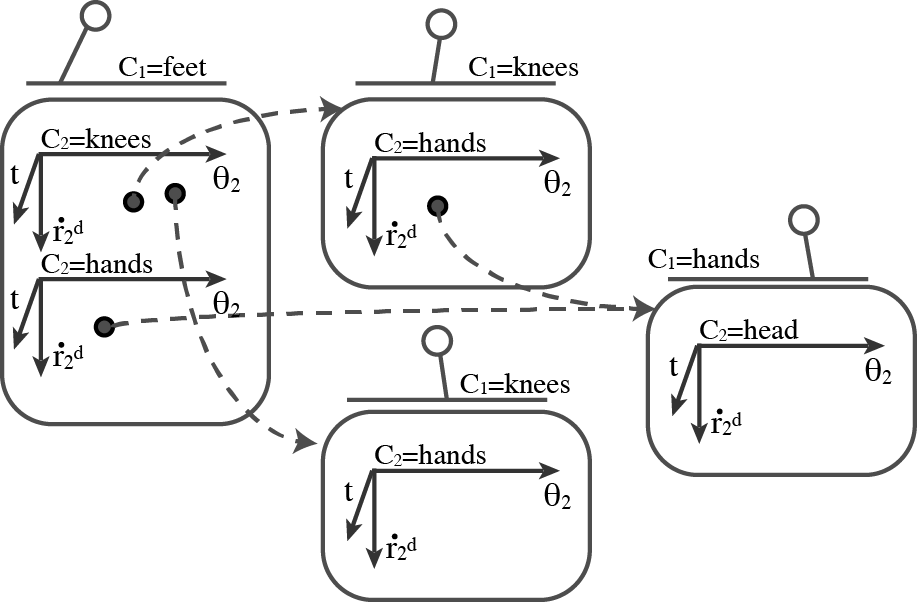
\includegraphics[width=3.2in]{images/recursive.png}
%%   \caption{\updated{We illustrate the concept of the
%%       recursive search by visualizing the states of pendulums (small drawings on boxes)
%%       and possible actions (4D tables in boxes).
%%       Note that different actions can possibley result the same state. }}
%%   \label{fig:falling_recursion}
%% \end{figure}

Our goal is to search for the best action sequence in $\mathcal{A}$ to
minimize the maximum impulse. The long-term cost of an action $\vc{a}$
taken at a state $\vc{x}$ can be expressed as
\begin{equation}
\max\big(g(\vc{x}, \vc{a}), v(f(\vc{x}, \vc{a}))\big),
\label{eq:falling_actionEval}
\end{equation}
where $g(\vc{x}, \vc{a})$ is the local cost function which computes
the vertical impulse due to the action $\vc{a}$ taken at the state
$\vc{x}$, $f(\vc{x}, \vc{a})$ is the transition function which outputs
the state after taking $\vc{a}$ at $\vc{x}$, and $v(\vc{x})$ is
the $cost \mhyphen to \mhyphen go$ function that yields the minimal impulse starting from
$\vc{x}$ following the best actions. The cost-to-go function can be
expressed recursively as
\begin{equation}
v(\vc{x}) = \min_{\vc{a}} \max(g(\vc{x}, \vc{a}), v(f(\vc{x}, \vc{a}))).
\label{eq:falling_cost-to-go}
\end{equation}
Determining the best action from a given state is a 4D search
problem. Every evaluation of an action (\eqnref{falling_actionEval}) invokes a
cost-to-go function (\eqnref{falling_cost-to-go}), which recursively generates
another 4D search problem. Although the recursive
search exponentially expands with the number of contacts, the state
space we need to consider is quite limited due to the monotonicity
nature of falling motion. That is, as the robot falls, $\theta_1$
changes monotonically from the initial value to $0$ (or
$\pi$). Likewise, $\dot{\theta}_1$ will never exceed the range between
the initial velocity and $0$. As a result, the algorithm visits a
large number of repeated states during the search. We exploit this
property using dynamic programming with k-nearest neighbor algorithm
to significantly expedite the search (details later).

\begin{algorithm}
  \If {$\dot{\theta}_1<0$} {
    \Return $0$\; 
    \label{alg:line:falling_terminal}
  }
  \If {kNN has $\vc{x}$}
      { \label{alg:line:falling_knn_query} 
        \Return $kNN[\vc{x}]$\;
      }
      $\bar{j} = \infty$\;
      \For {$\dot{r}_1^d \in \mathcal{V}$} { \label{alg:line:falling_rdot}
        $\vc{x}^{now}=\vc{x}$\;
        $\Delta t=0$\;
        \While {$\theta_1^{now} < \pi/2$} { \label{alg:line:falling_theta}
          $\mathcal{S} = generate\_stoppers(\vc{x}^{now}, \Delta t)$\; \label{alg:line:falling_collect}
          \For {$c_2, \theta_2 \in \mathcal{S}$} {
            $\vc{a}=\{(c_2, \theta_2, \Delta t, \dot{r}_1^d)\}$\;
            $\vc{x}^{+}=f(\vc{x}^{now}, \vc{a}$)\;
            $ j^{+}=g(\vc{x}^{now}, \vc{a}$)\;
            $j^{*}$ = $cost \mhyphen to \mhyphen go(\vc{x}^{+})$\;
            $\bar{j}$ = $\min(\bar{j}, \max{(j^{+}, j^{*})})$\;
          }
          $\vc{x}^{now}$ = $simulate\_pendulum(\vc{x}^{now}, \dot{r}_1^d$)\; \label{alg:line:falling_sim}
          $\Delta t = \Delta t + h$\;
        }
      }
      $kNN[\vc{x}]=\bar{j}$\; \label{alg:line:falling_knn_save} 
      \Return $\bar{j}$\;
      \caption{$cost \mhyphen to \mhyphen go(\vc{x})$}
      \label{alg:falling_recursive}
\end{algorithm}


\begin{algorithm}
  $\mathcal{S}$ = $\emptyset$\;
  %% $(r_1, \theta_1) = (r_1(\vc{x}), \theta_1(\vc{x}))$\;
  \For{$c_2\in\{c_2 \vert (c_1 \rightarrow c_2)\in E_{c} \}$} {
    \For{$\theta_2 \in [-\pi, \pi]$} {
      $r_2 = r_1 cos(\theta_1) / -cos(\theta_1 + \theta_2)$\;
      %% \If {not valid\_kinematics($r_1$, $r_2$, $\theta_2$)} {
      \If {$\mathcal{K}_{c_1\rightarrow c_2}[r_1][r_2][\theta_2] = 0$}{ \label{alg:line:falling_kinematic} 
        continue\;
      }
      %% \If {not valid\_dynamics($t$, $\theta_2$, $c_1$, $c_2$)} {
      \If {$|\theta_2 - \hat{\theta}_2(c_1,c_2)| > (\hat{t} + \Delta t) \dot{\theta}_{max}$}{ \label{alg:line:falling_temporal} 
        continue\;
      }
      $\mathcal{S} = \mathcal{S} \cup \{(c_2, \theta_2)\}$\;
    }
  }
  \Return $\mathcal{S}$\;
  \caption{generate\_stoppers($\vc{x}, \Delta t$)}
  \label{alg:falling_stopper}
\end{algorithm}

%% The full algorithm is shown in \algref{falling_recursive}.
\algref{falling_recursive} shows the evaluation of the cost-to-go
function. For a given state $\vc{x}$, we search in the 4D action space
with respect to the bounds in each dimension. The range of the desired
rod velocity ($\dot{r}^d_1$) is based on the specifications of the robot
(\lineref{falling_rdot}). The elapse time between two consecutive impact
moments ($\Delta t$) is bounded by the time that takes the pendulum to
fall from $\theta_1$ to the ground (\lineref{falling_theta}).  The actual
range of $\Delta t$ depends on a forward simulation process
(\lineref{falling_sim}). The candidates of $c_2$ are defined by the contact
graph and the corresponding range of $\theta_2$ for each candidate is
determined by the kinematic limits of the robot. $c_2$ and $\theta_2$
together define a set of feasible stoppers, $\mathcal{S}$, for the
next contact (\lineref{falling_collect}). \algref{stopper} describes the
details on generating the feasible stopper set.

The feasibility of the stopper depends on whether the robot can
achieve the kinematic constraints imposed by $r_1$, $r_2$, $\theta_2$
for a particular contact transition from $c_1$ to $c_2$
(\lineref{falling_kinematic}).  Instead of solving an inverse kinematic
problem, we expedite the feasibility test by building lookup tables as
a preprocess. We first create $10000$ distinctive random
configurations of the robot within its joint limits. For each
connected pair of nodes $(c_1, c_2)$ in the contact graph, we create a
3D lookup table
$\mathcal{K}_{c_1\rightarrow c_2}[r_1][r_2][\theta_2]$. If the
attributes of an entry (\ie $r_1$, $r_2$, and $\theta_2$) match $r_1$,
$r_2$, and $\theta_2$ extracted from one of the $10000$ robot
configurations within tolerance intervals, we mark that entry one, and
zero otherwise. With this lookup table, we can efficiently accept or
reject a proposed stopper based on the kinematic constraints of the
robot.

In addition, we need to make sure that the stopper can reach the
proposed $\theta_2$ within $\hat{t} +\Delta t$ second from its initial
position, $\hat{\theta}_{2}(c_1,c_2)$, at the beginning of the
fall. For each pair of connected contact points $(c_1, c_2)$ on the
contact graph, we precompute the angle $\hat{\theta}_{2}(c_1,c_2)$,
defined as the angle between the vector from $c_1$ to COM and the
vector from COM to $c_2$, on the initial configuration of the robot.
If the proposed $\theta_2$ cannot be achieved by moving at the maximum
speed in $\hat{t} +\Delta t$ seconds, we reject the proposed stopper
(\lineref{falling_temporal}).


% The
% initial position of the stopper can be arbitrarily defined because the
% stopper is uncontrolled and irrelevant to the algorithm until the
% previous contact ($c_1$) is activated.
%% \sehoon{Will it be better to include time $t$ in the tip state
%%   $\vc{x}$?}
%% \karen{I don't see why it is necessary.}
%% \sehoon{This bound will not be accurate, as you claimed.
%%   $c_1$ and $c_2$ will keep changing in the sequence, 
%%   so $\theta_2^0[c_1][c_2]$ will be less useful afterward.
%%   However, this will be just a rough bound that removes the very unrealistic
%%   stoppers. 
%%   A tight bound will be much difficult to model because exactly same 
%%   ($c_1, c_2, r_1, r_2, \theta_2$) can be very different in the fullbody
%%   poses. 
%%   It might be good to discuss this in the limitation section..}
%% \karen{Yes. We need to discuss this in the limitation section.}

Whenever we need to evaluate the cost-to-go of a new state, we first
check whether there exists a previously visited state sufficiently
close to the new state. If so, the cost-to-go of the previously
visited state is returned (\lineref{falling_knn_query}). If not, we
recursively expand the search to the next contact.  The similarity
function measures the Euclidean distance between two states weighted
by $\vc{w}=[100.0, 1.0, 1.0, 0.1, 2.0, 4.0]$ to account for the
different units in different dimensions of the state space.

\algref{falling_recursive} terminates when the velocity of the pendulum is
zero or negative (\lineref{falling_terminal}), indicating that the initial momentum is
completely dissipated. After the termination, we do a forward pass to
recover the sequence of contacts by following the best actions. For
each contact $i$, we record the state at the impact moment
$\vc{x}^{(i)}$ and the optimal action $\vc{a}^{(i)}$ that leads to the
state of the next impact moment $\vc{x}^{(i+1)}$. We define the
contact plan as
$\mathcal{P} = \{ (\vc{x}^{(1)}, \vc{a}^{(1)}) \cdots (\vc{x}^{(k)},
\vc{a}^{(k)}) \}$, where $k$ is the total number of contacts.


% The best action
% for the 4D search problem of contact $i$ suggests the state of the
% pendulum when the stopper is optimally activated and the optimal
% stopper $(\vc{x}^{(i)}, \vc{a}^{(i)})$.
%%%%%%%%%%%%%%%%%%%%%%%%%%%%%%%%%%%%%%%%%%%%%%%%%%%%%%%%%%%%%%%%%%%%%%%%%%%%%%%%
\paragraph{Plan for whole-body motion}
The final step is to execute the contact plan solved by
\algref{falling_recursive} on the humanoid robot.  Our approach is to solve
for a sequence of whole-body configurations,
$\vc{q}^{(1)}, \cdots, \vc{q}^{(k)}$, to match the contact
plan. 
$\vc{q}^{(i)}$ is defined as a set of actuated joint angles
which will be tracked by the robot during contact $i$ using PID
control. For each $(\vc{x}^{(i)}, \vc{a}^{(i)})$ in $\mathcal{P}$, we
formulate an optimization problem as follows:
\begin{multline}
  \vc{q}^{(i)} = \argmin_{\vc{q}} \Big(
  \|\vc{z}(\vc{q}, c_1^{(i)}) - \vc{p}_0\|^2 +
  \|\vc{c}(\vc{q}) \\ - \vc{p}_1(\vc{x}^{(i)})\|^2 + 
  \|\vc{z}(\vc{q}, c_2^{(i)}) - \vc{p}_2(\vc{x}^{(i)}, \vc{a}^{(i)})\|^2  
  \Big).
\end{multline}
The first term in the objective function tries to match the current
contact position of the robot, $\vc{z}(\vc{q}, c_1^{(i)})$, to the
pivot of the abstract model, $\vc{p}_0$.
The second term tries to
match the COM of the robot, $\vc{c}(\vc{q})$, to the
position of the pendulum, $\vc{p}_1(\vc{x}^{(i)})$. Finally, the
third term tries to match the next contact position of the robot,
$\vc{z}(\vc{q}, c_2^{(i)})$, to the tip of the stopper,
$\vc{p}_2(\vc{x}^{(i)}, \vc{a}^{(i)})$.  After solving the optimal
sequence of poses, the robot is commanded to track the pose
$\vc{q}^{(i)}$ from the beginning of contact $c_1^{(i)}$ to the
beginning of contact $c_2^{(i)}$.


%% \karen{Did other researchers use the term ``robot'' or ``humanoid'' or ``biped''
%%   in the papers?}
%% \karen{Need to explain how we define $\vc{p}_0$.}

%%%%%%%%%%%%%%%%%%%%%%%%%%%%%%%%%%%%%%%%%%%%%%%%%%%%%%%%%%%%%%%%%%%%%%%%%%%%%%%%
%%%%%%%%%%%%%%%%%%%%%%%%%%%%%%%%%%%%%%%%%%%%%%%%%%%%%%%%%%%%%%%%%%%%%%%%%%%%%%%%
\section{Experiments}
We evaluated our multiple contact planning algorithm on two simulated
humanoids, BioloidGP \cite{BioloidGP:2014:URL} and Atlas
\cite{BD:2014:URL}, as well as the actual hardware of BioloidGP.  Our
algorithm was compared against a naive approach without planning--the
robot simply tracks the initial pose throughout the fall. For the two
simulation settings, our evaluation metric is the maximum impulse as
previously defined. For the hardware experiments, we measured the maximum
acceleration of the head.

  %% We also compared changes of strategies for the different perturbations 
  %% to show the versatility of our approach. 

%%%%%%%%%%%%%%%%%%%%%%%%%%%%%%%%%%%%%%%%%%%%%%%%%%%%%%%%%%%%%%%%%%%%%%%%%%%%%%%%
\subsection{Simulation Results}
We used an open source physics engine, DART
\cite{DART:2014:URL,Liu:2012:STM} with 0.0005s time step ($h$) to
simulate the motion of the humanoids.  Contacts and collisions were
handled by an implicit time stepping, velocity-based LCP
(linear-complementarity problem) to guarantee non-penetration,
directional friction, and approximated Coulomb friction cone
conditions.
%% Our algorithm evaluates $500$ to $3000$ states and takes $1.0$ to $10.0$
%% seconds.\karen{Move this to limitation.}

%% \begin{figure}[ht]
%% \center
%%   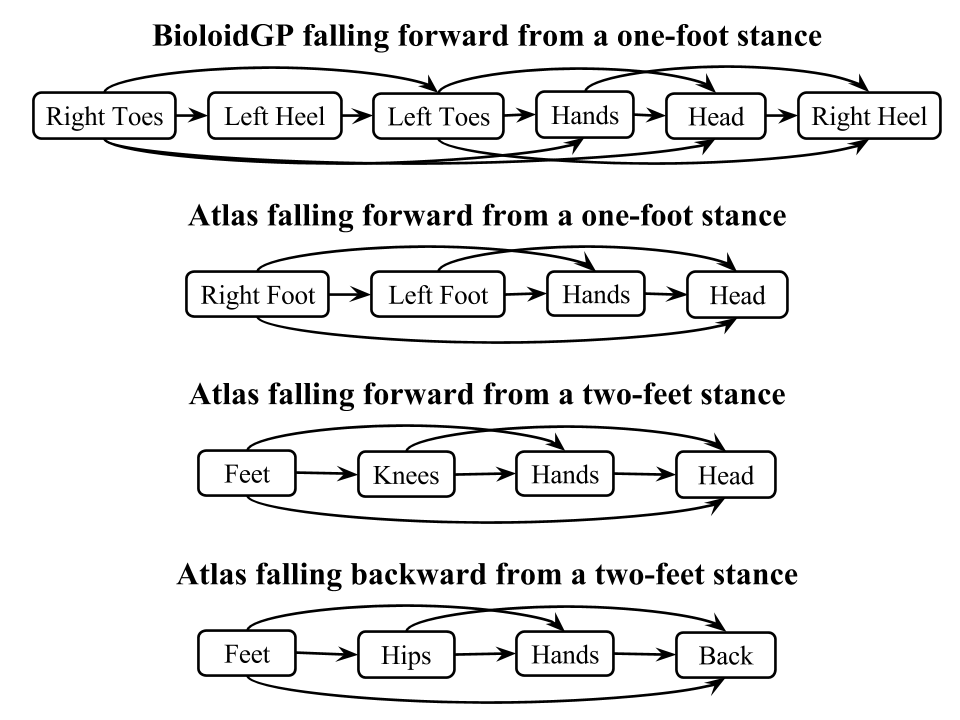
\includegraphics[width=3.2in]{images/all_contact_graphs.png}
%%   \caption{\updated{More contact graphcs are represented.
%%       Top: a forward fall of BioloidGP from one feet
%%       Middle: a forward fall of Atlas from one feet
%%       Bottom: a backward fall of Atlas from two feet}
%%     \sehoon{Will it be better to merge this with the previous contact graph
%%       figure (Figure. 2)?}}
%%   \label{fig:falling_all_contact_graphs}
%% \end{figure}

\begin{figure*}[ht]
\center
  %% 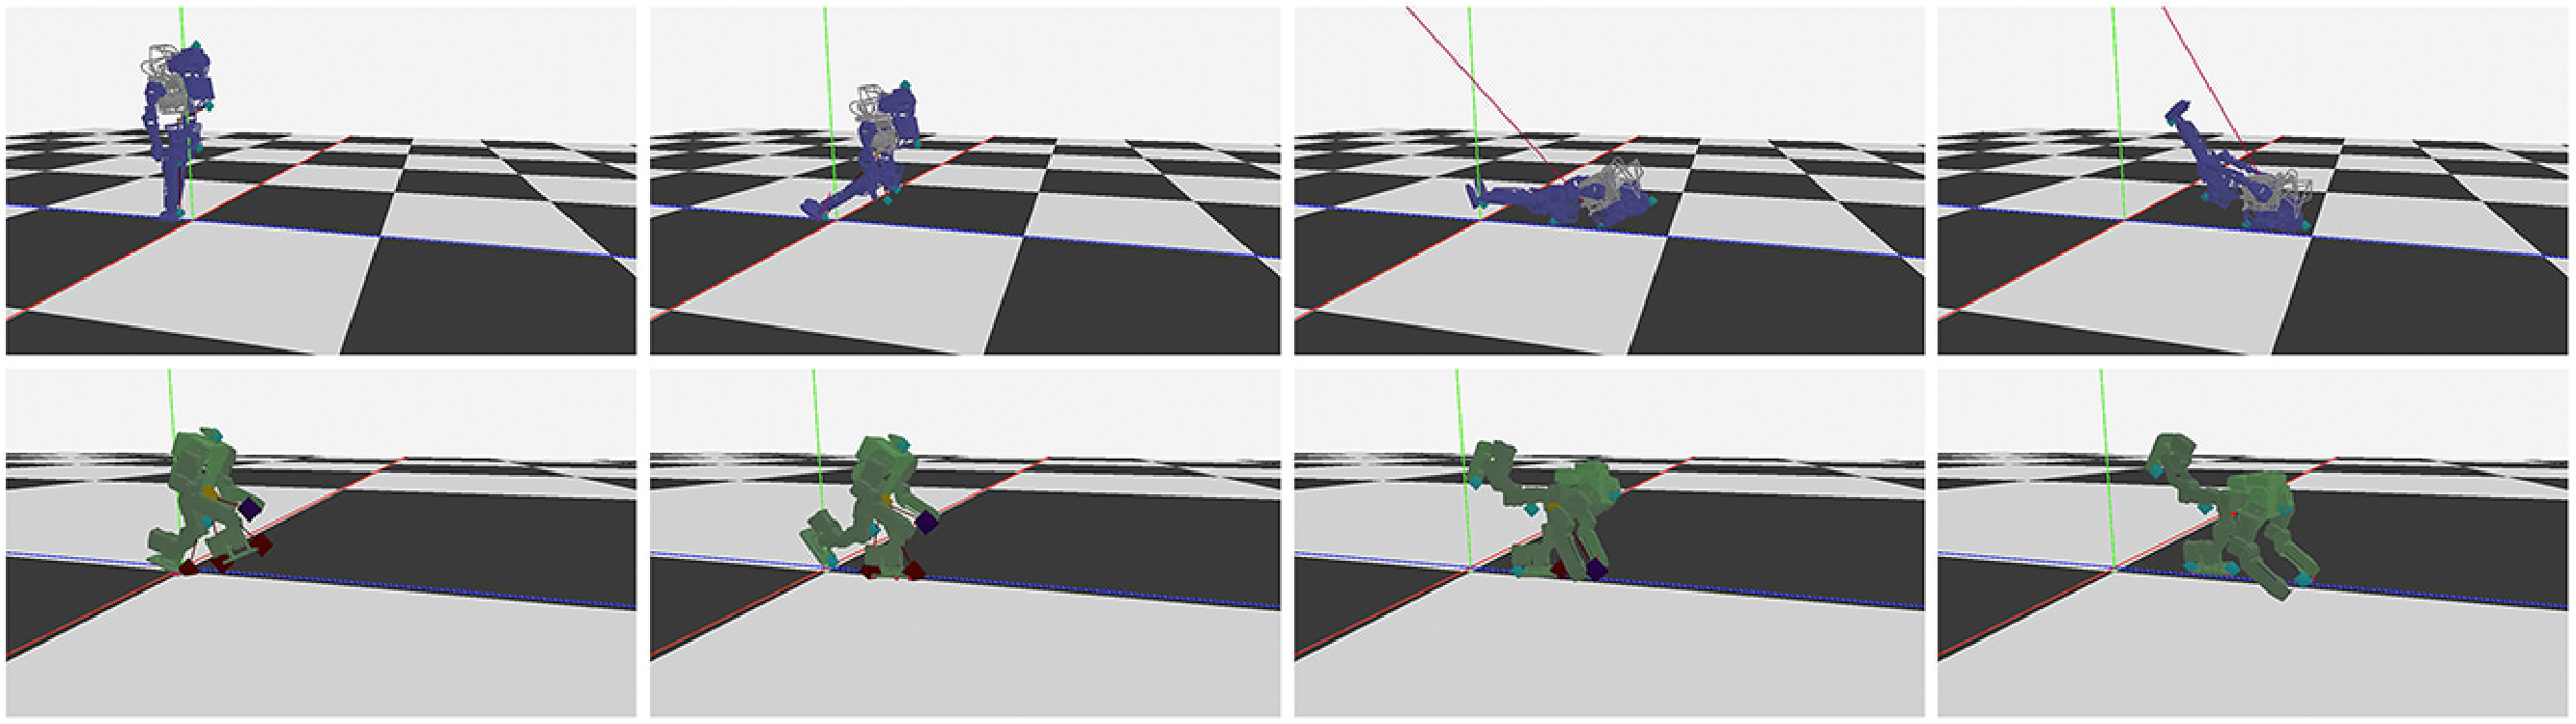
\includegraphics[width=6.8in]{images/falling_motions.pdf}
\setlength{\tabcolsep}{1pt}
\renewcommand{\arraystretch}{0.5}
\begin{tabular}{c c c c}
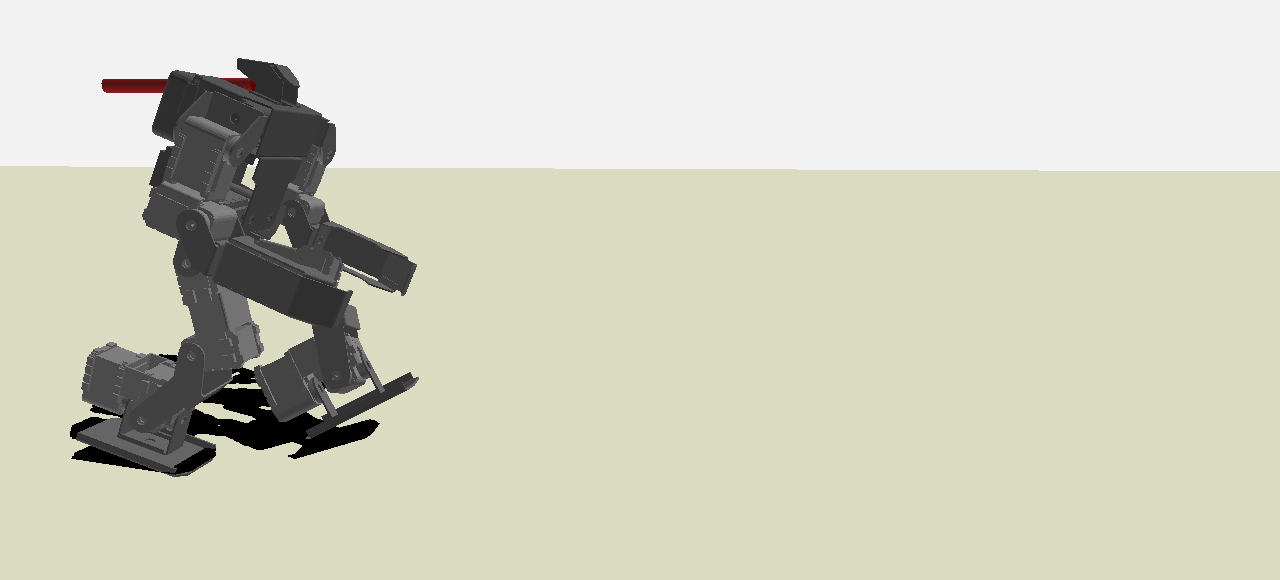
\includegraphics[width=0.24\textwidth]{images/GP_A_0.png}&
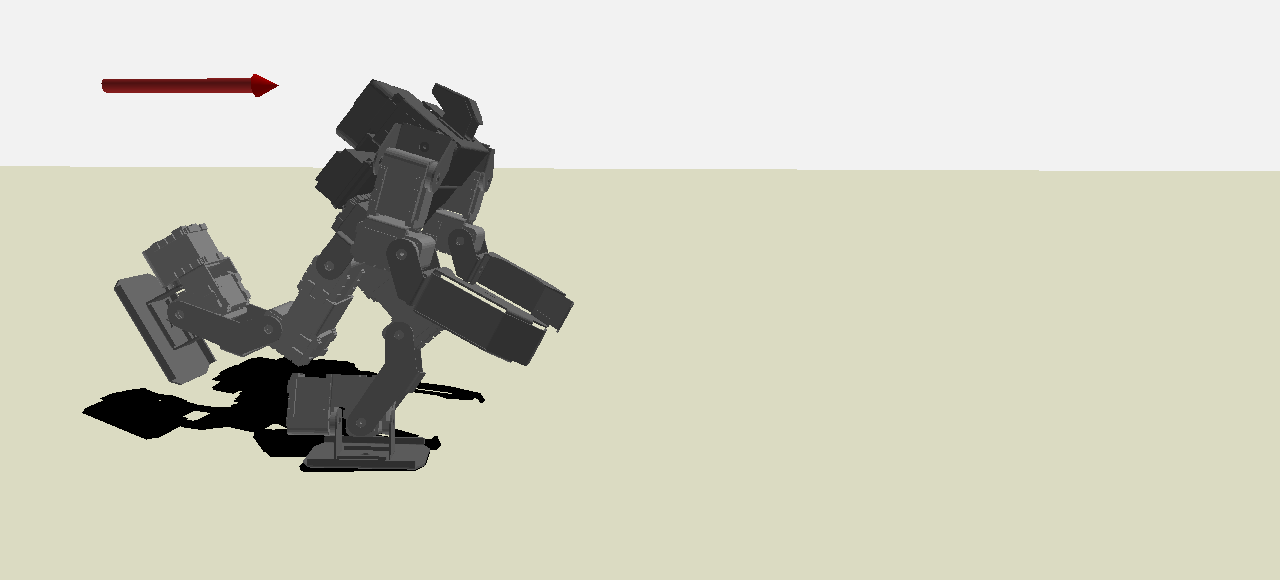
\includegraphics[width=0.24\textwidth]{images/GP_A_1.png}&
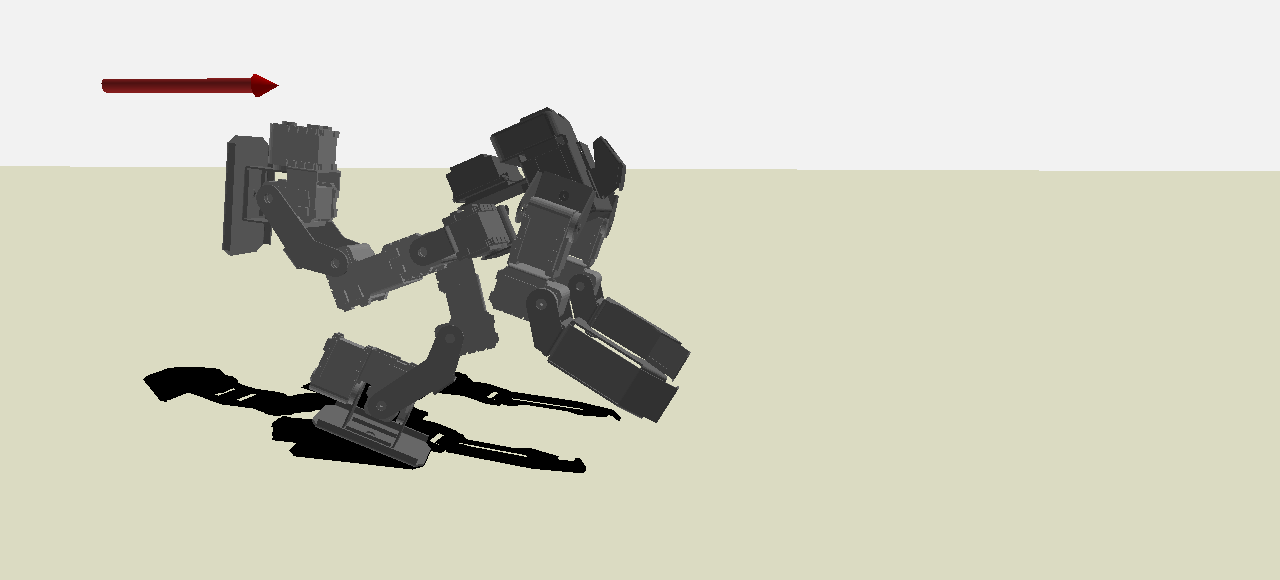
\includegraphics[width=0.24\textwidth]{images/GP_A_2.png}&
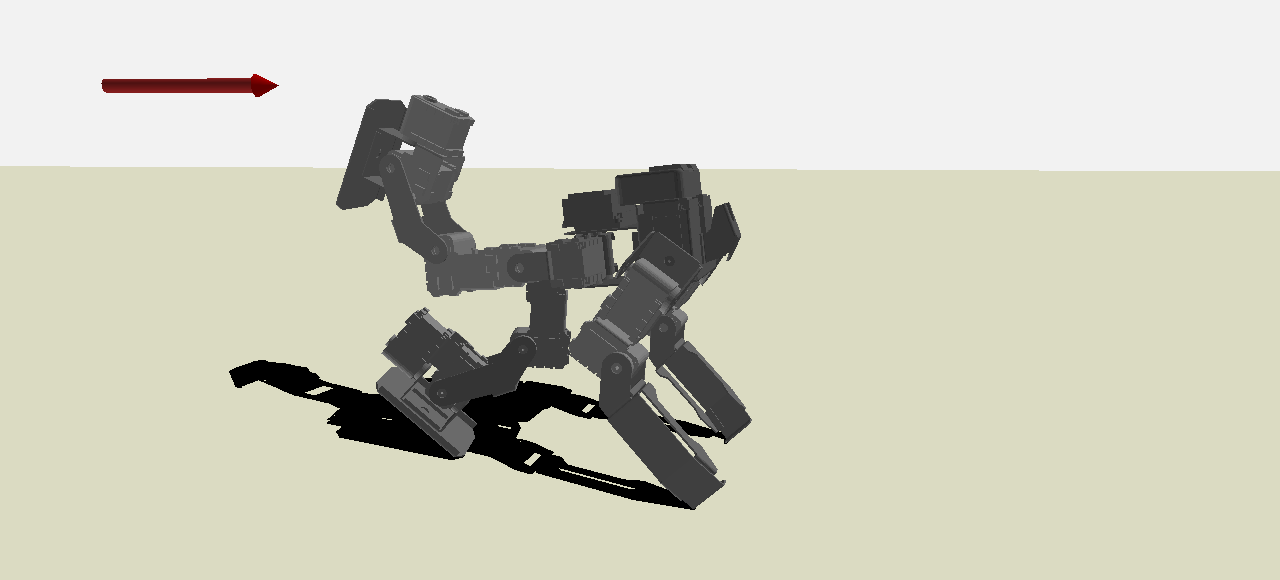
\includegraphics[width=0.24\textwidth]{images/GP_A_3.png} \\
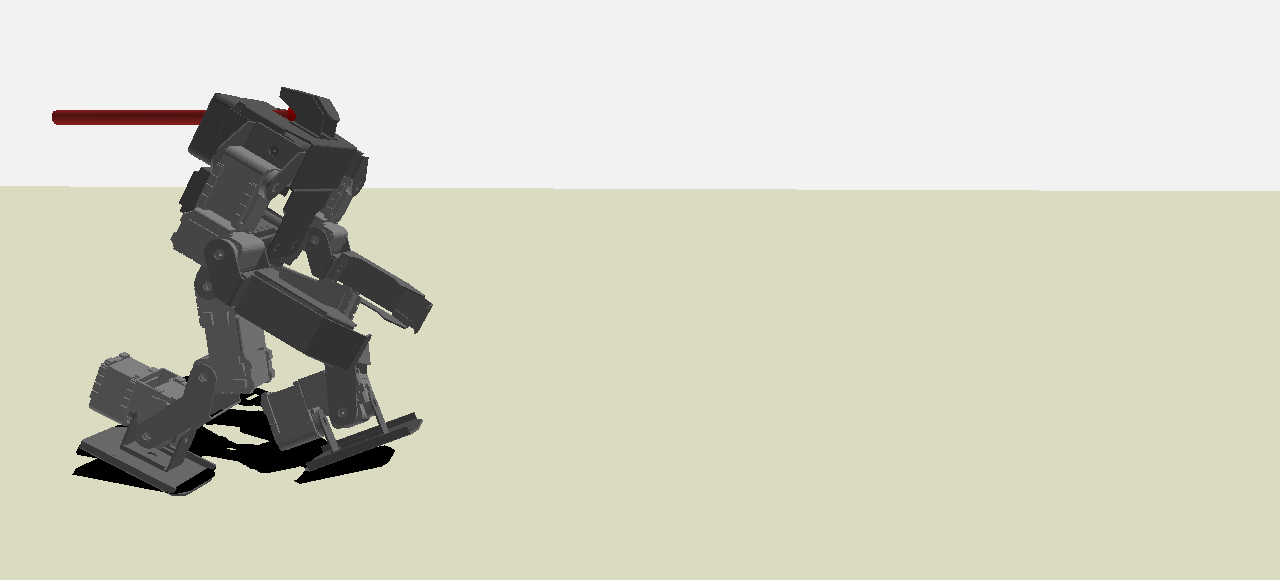
\includegraphics[width=0.24\textwidth]{images/GP_B_0.png}&
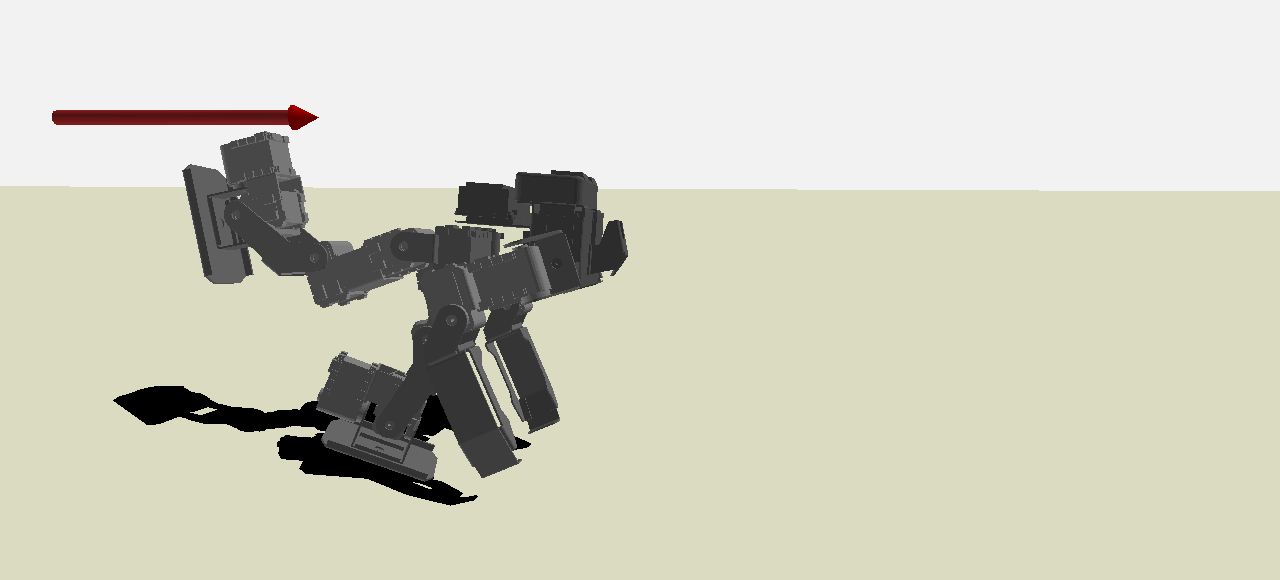
\includegraphics[width=0.24\textwidth]{images/GP_B_1.png}&
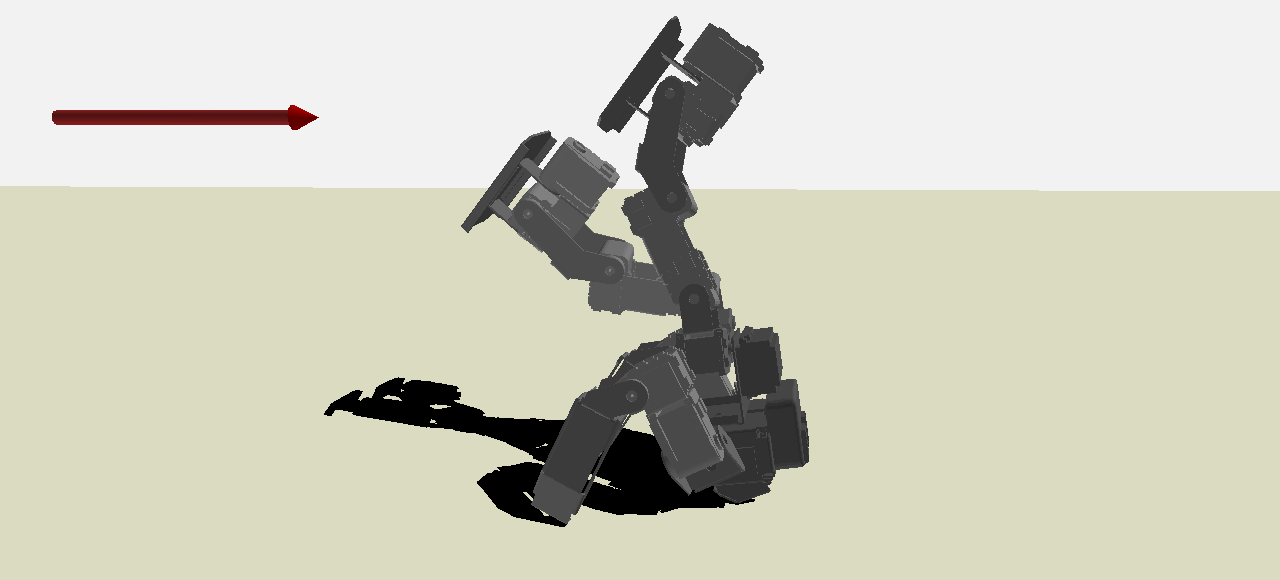
\includegraphics[width=0.24\textwidth]{images/GP_B_2.png}&
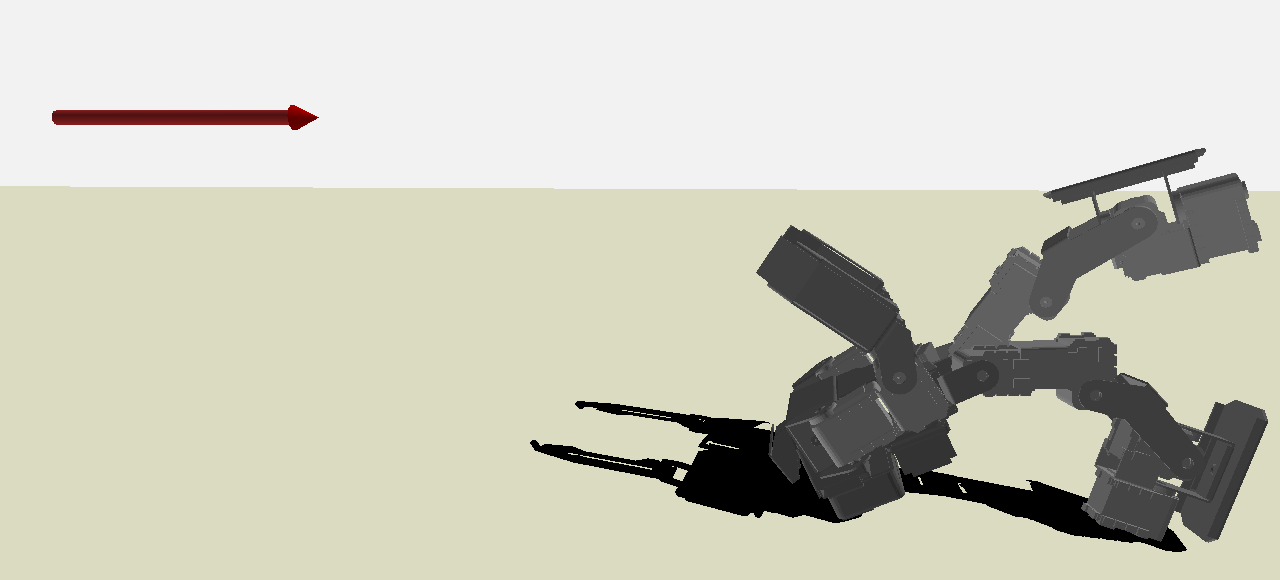
\includegraphics[width=0.24\textwidth]{images/GP_B_3.png} \\
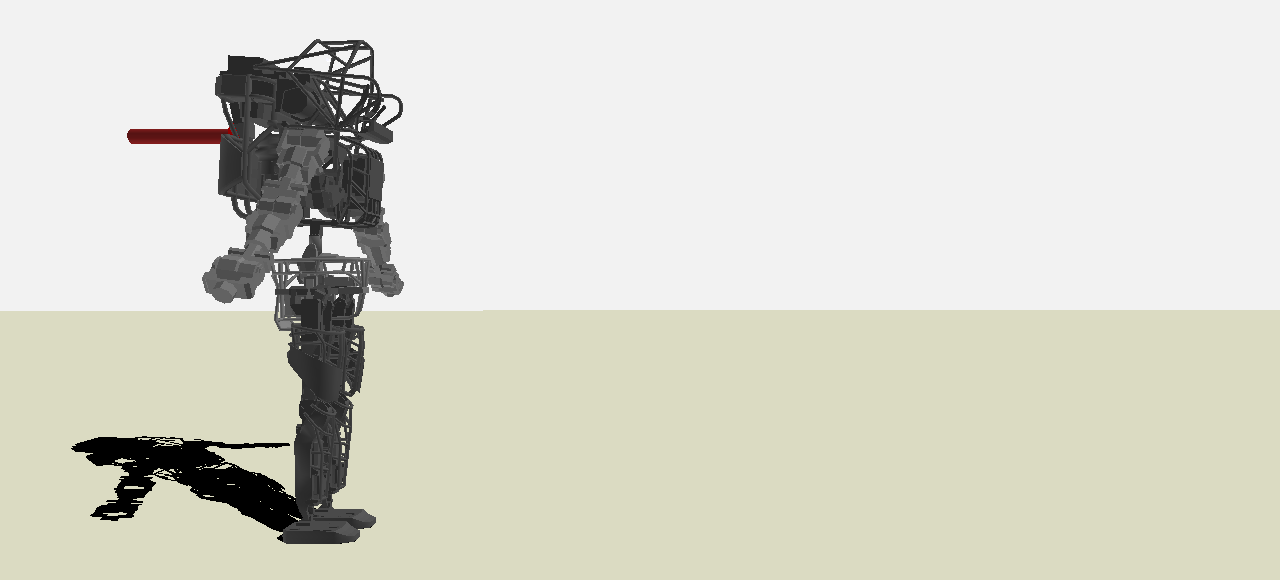
\includegraphics[width=0.24\textwidth]{images/Atlas_A_0.png}&
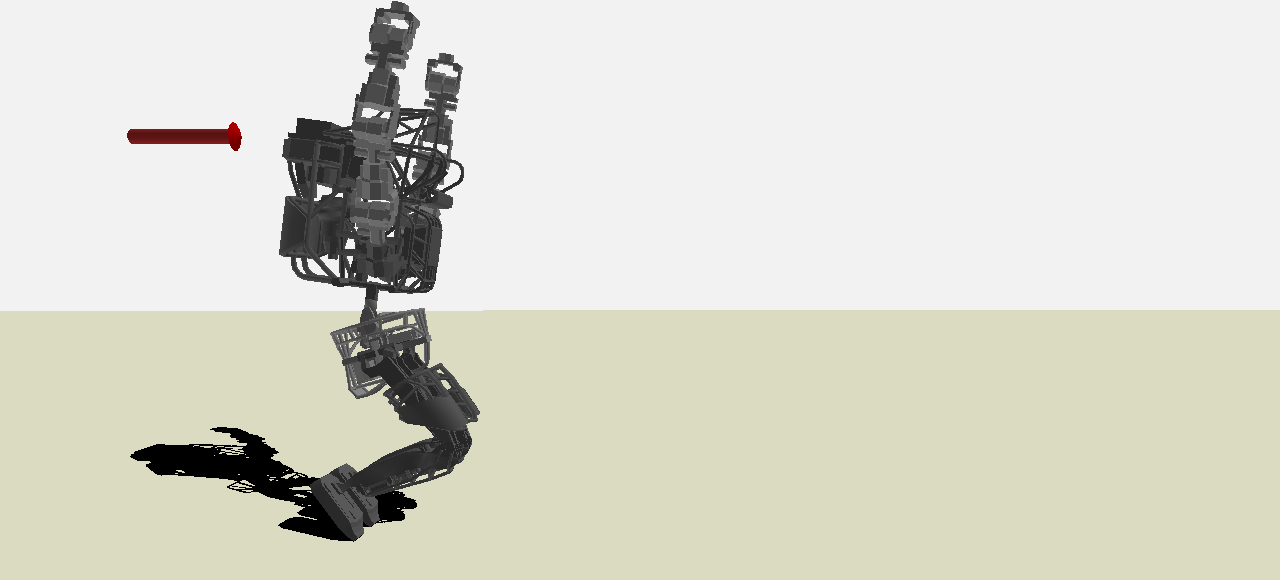
\includegraphics[width=0.24\textwidth]{images/Atlas_A_1.png}&
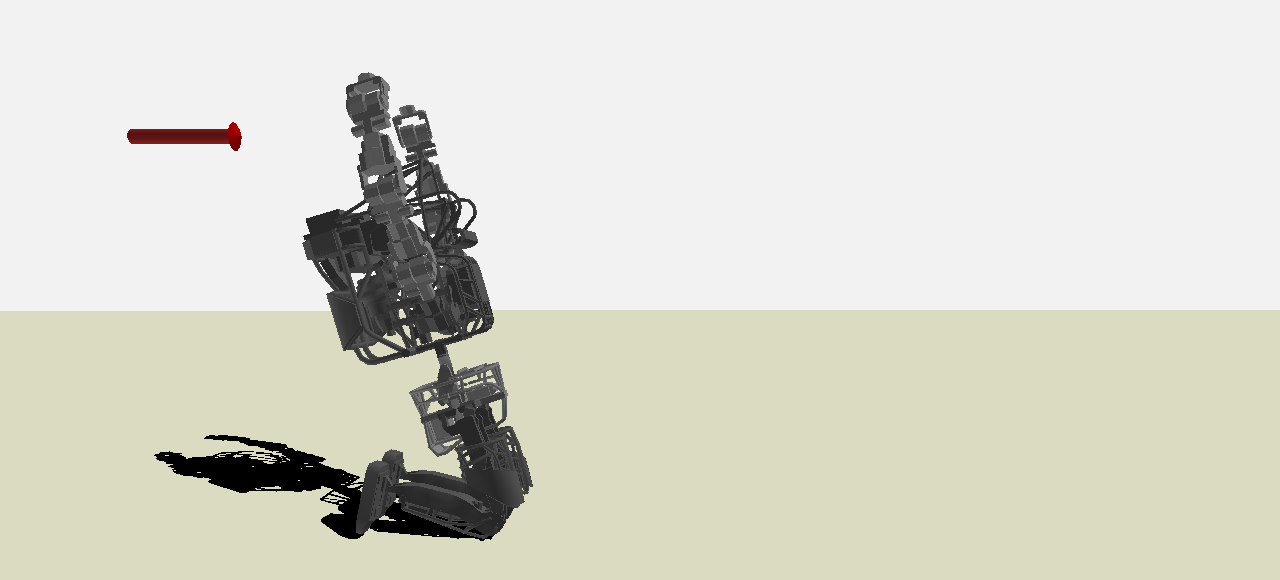
\includegraphics[width=0.24\textwidth]{images/Atlas_A_2.png}&
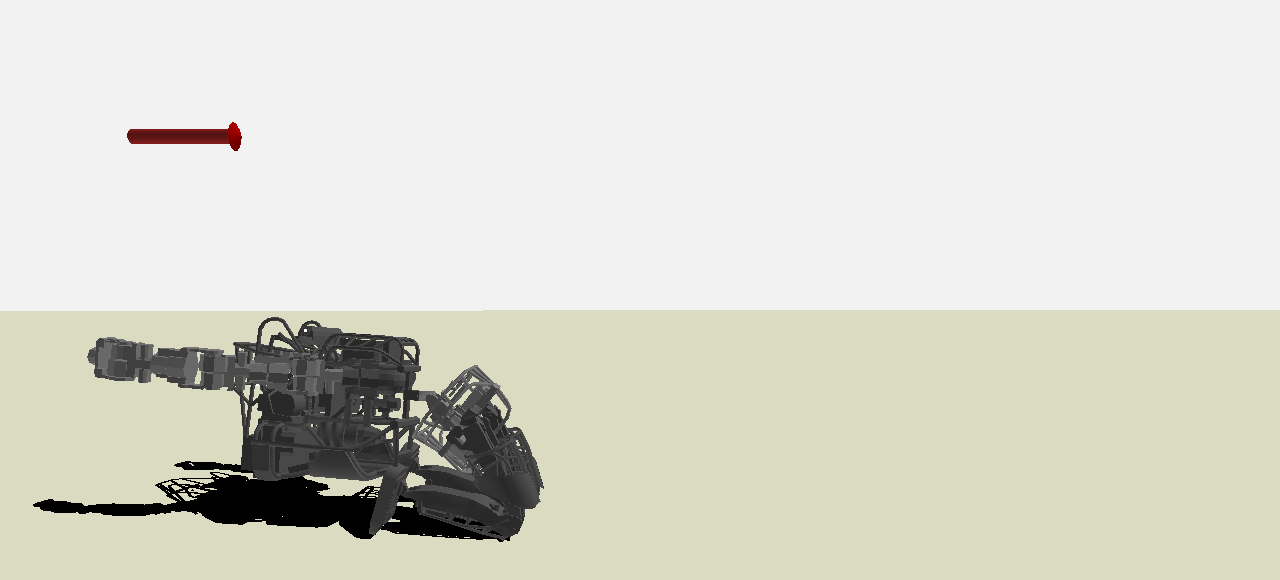
\includegraphics[width=0.24\textwidth]{images/Atlas_A_3.png} \\
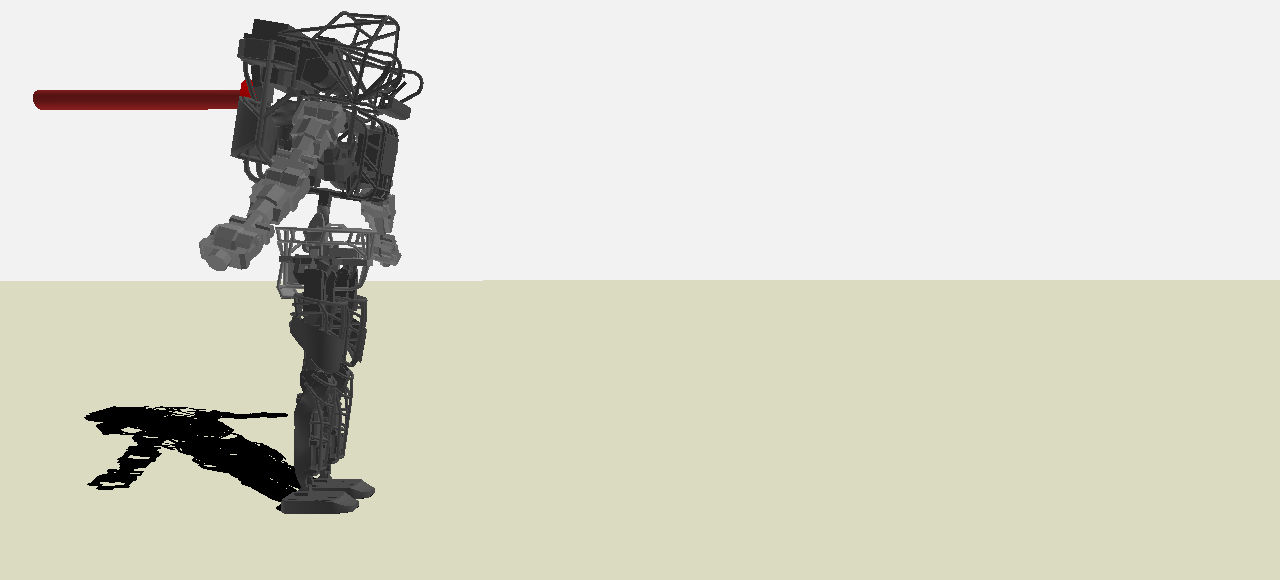
\includegraphics[width=0.24\textwidth]{images/Atlas_B_0.png}&
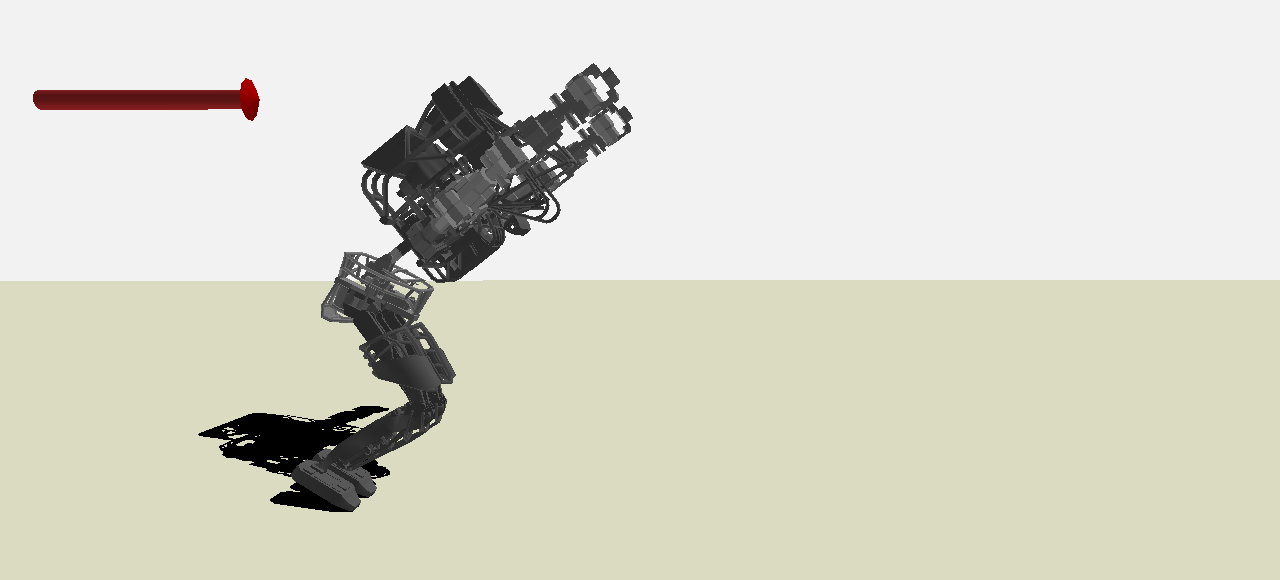
\includegraphics[width=0.24\textwidth]{images/Atlas_B_1.png}&
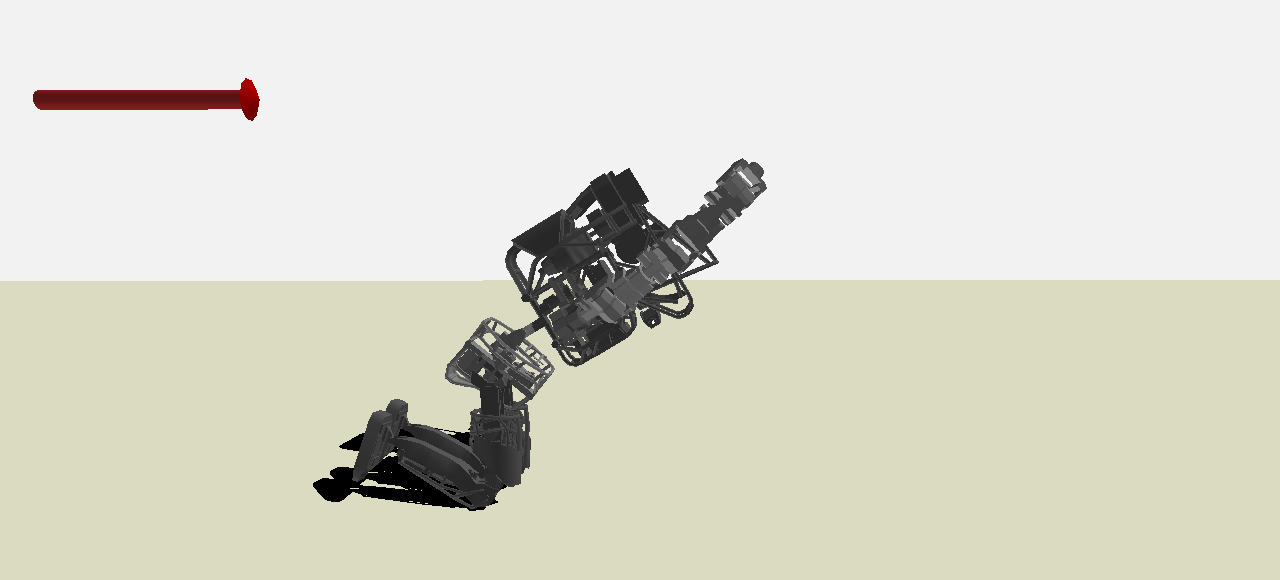
\includegraphics[width=0.24\textwidth]{images/Atlas_B_2.png}&
\includegraphics[width=0.24\textwidth]{images/Atlas_B_3.png} \\
\end{tabular}
\caption{First row: BioloidGP forward falling from a one-foot
    stance due to a $5.0$N push. Second row: BioloidGP forward falling
    from a one-foot stance due to a $8.0$N push. Third row: Atlas
    forward falling from a two-feet stance due to a $1000$N push. Fourth
    row: Atlas forward falling from a two-feet stance due to a
    $2000$N push.}
  \label{fig:falling_motions}
\end{figure*}

%%%%%%%%%%%%%%%%%%%%%%%%%%%%%%%%%%%%%%%%%%%%%%%%%%%%%%%%%%%%%%%%%%%%%%%%%%%%%%%%
\subsubsection{BioloidGP}
BioloidGP is a small humanoid robot with $16$ degrees of freedom (DOFs)
($34.6$cm, $1.6$kg). Our first set of tests applied pushes with
different magnitudes to the robot. Starting with the same one-foot
stance, we ran four tests with pushes ranging from $0.5$N to $8.0$N,
applied for $0.1$ second at beginning of the fall. We set the joint
angle limits at $\pm150^{\circ}$ and the torque limits at $0.6Nm$. We
approximated the speed limit of the COM in the vertical direction and
set the limits of the rod length velocity $\dot{r}_1^d$ at
$\pm0.03m/s$. The input contact graph is shown in
\figref{falling_contact_graph}.  Due to the relatively large feet of
BioloidGP, heels and toes were treated as two separate contacts.

%% \sehoon{How about denote ``\# of contacts'' in \tabref{falling_gp_results}
%%   instead of the full sequence of contacts? In that case, we can make
%%   the table as one column. We can explain the sequence in the text and
%%   video.}
%% \karen{I like the entire contact sequence in the table, unless we need
%%   to save space.}

%%%%%%%%%%%%%%%%%%%%%%%%%%%%%%%%%%%%%%%%
% Table begins
\begin{table*}
\scriptsize
\center
{
\caption{The initial conditions and the results of BioloidGP simulations.
}
\begin{tabular}{c |c c c|l | l}
\label{tab:falling_gp_results}
\\ \hline
Mag.(N) & Unplanned & Planned & Ratio & Contacts & Remarks \\ \hline
0.5 & 0.8889 & 0.2063 & 23.2\% & right toes, left heel, left toes & Stepping\\ \hline
1.5 & 0.6789 & 0.2776 & 40.9\% & right toes, left heel, left toes, hands & Tripod\\ \hline
5.0 & 0.9312 & 0.3885 & 41.7\% & right toes, left heel, left toes, hands & Tripod \\ \hline
8.0 & 1.2170 & 0.5884 & 48.4\% & right toes, left heel, left toes, hands, head, right heel & Rolling \\ \hline
\end{tabular}
}
\end{table*}
%%%%%%%%%%%%%%%%%%%%%%%%%%%%%%%%%%%%%%%%
\tabref{falling_gp_results} describes the details of the initial conditions
and the results of each test. The columns of the table denote the
magnitude of perturbation, the maximum impulses of the unplanned and
the planned motions, the impact ratio of planned to unplanned motion,
the optimal contact sequence, and a short description of the
emergent falling strategy. As we expected, our planning algorithm used more
contacts when the initial momentum was large. For a push with $0.5$N,
the robot took a single step to recover the fall. For the cases of
$1.5$N and $5.0$N, our algorithm planned a contact sequence with the
left heel, the left toe, and both hands, reminiscent to the Tripod strategy
proposed by \cite{Yun:2014:TFC}. When we increased the magnitude of the
push to $8.0$N, the rolling strategy, effective for breaking high
speed falls \cite{ZenpoUkemi:2014:URL}, automatically emerged. Please
refer to the supplementary video and \figref{falling_motions} for all the
results.

\begin{figure}[ht]
\center
  %% \includegraphics[width=6.8in]{images/falling_motions.pdf}
\setlength{\tabcolsep}{1pt}
\renewcommand{\arraystretch}{0.5}
\begin{tabular}{c c}
\includegraphics[width=2.2in]{images/COM_GP_A.png}&
\includegraphics[width=2.2in]{images/COM_GP_B.png}\\
\includegraphics[width=2.2in]{images/COM_Atlas_A.png}&
\includegraphics[width=2.2in]{images/COM_Atlas_B.png}\\
\end{tabular}

  \caption{COM trajectories between the abstract model
      (Blue) and the robot (Red). 
      Top left: BioloidGP forward falling from a one-foot stance due to a
      $5.0$N push. Top right: BioloidGP forward falling from a one-foot stance
      due to a $8.0$N push. Bottom left: Atlas forward falling from a two-feet
      stance due to a $1000$N push. Bottom right: Atlas forward falling 
      from a two-feet stance due to a $2000$N push.}
  \label{fig:falling_coms}
\end{figure}

Comparing to unplanned motions, our algorithm only caused $23.2\%$ to
$48.4\%$ of the maximum impulse. To verify how well the
contact plan $\mathcal{P}$ was executed, we compared the COM
trajectories between the abstract model and the robot
(\figref{falling_coms}). Most plans were executed well with an exception of the
$8.0$N case due to the accumulated errors over a longer motion
sequence. Still, in this case the maximum impulse was significantly
reduced due to the distribution of impulse over multiple contacts.

The contact graph is an important input that defines all possible
contact sequences for the given humanoid. We ran an additional test to
modify the contact graph of the BioloidGP robot. By removing the
``hands'' node, the $8.0$N push resulted in a hands-free rolling sequence.
  % The maximum impulse of the new motion is $0.9890$Ns that is between the
  % original strategy ($0.5884$Ns) and the unplanned motion ($1.2170$Ns).}
  %% However, it results the higher maximum impulse ($0.9890$Ns) than the original
  %% strategy ($0.5884$Ns) that is still lower than the unplanned motion
  %% ($1.2170$Ns). }

%%%%%%%%%%%%%%%%%%%%%%%%%%%%%%%%%%%%%%%%%%%%%%%%%%%%%%%%%%%%%%%%%%%%%%%%%%%%%%%%
\subsubsection{Atlas}
We also evaluated our algorithm on a large humanoid, Atlas ($188$cm,
$150$kg, $28$DOFs).  We followed the joint limits and the torque
limits described in the URDF file provided by Boston Dynamics
\cite{BD:2014:URL}. The limits of the rod length velocity
$\dot{r}_1^d$ were set at $\pm0.3m/s$.  We ran six test cases with
three initial settings: a forward push from a one-foot stance pose, a
forward push from a two-feet stance pose, and a backward push from a
two-feet stance pose. For each setting, we pushed the robot with two
different magnitudes.  The input contact graphs are shown in
\figref{falling_contact_graph}.

%%%%%%%%%%%%%%%%%%%%%%%%%%%%%%%%%%%%%%%%
% Table begins
\begin{table*}
\scriptsize
\center
{
\caption{The initial conditions and the results of Atlas simulations.}
\begin{tabular}{c c c|c c c| l }
\label{tab:falling_atlas_results}
\\ \hline 
Initial Stance & Direction & Mag.(N) & Unplanned(Ns) & Planned(Ns) & Ratio & Contacts \\ \hline
One foot & Forward & 1000 & 363.9 & 37.8 & 10.4\% & right foot,  left foot \\ \hline
One foot & Forward & 2500 & 401.5 & 281.1 & 70.0\% & right foot,  left foot, hands \\ \hline
Two feet & Forward & 1000 & 392.8 & 214.0 & 54.5\% & feet, knees \\ \hline
Two feet & Forward & 2000 & 322.7 & 199.7 & 61.8\% & feet, knees, hands \\ \hline
Two feet & Backward & 300 & 338.8 & 176.5 & 52.1\% & feet, hands \\ \hline
Two feet & Backward & 500 & 344.6 & 243.9 & 70.8\% & feet, hips, hands, back \\ \hline
\end{tabular}
}
\end{table*}

\tabref{falling_atlas_results} shows the initial settings and the results for all
the tests. Again, our algorithm suggested to use more contacts for
pushes with higher magnitudes. For the same setting (falling forward
from a one-foot stance pose), we observed a change of strategy from taking a
small step ($1000N$) to using Tripod strategy ($2500N$).  In the case
of falling forward from a two-feet stance pose, the robot landed on its knees
when the push was weak ($1000N$), similar to the strategy proposed by
\cite{Fujiwara:2004:SKL}.  When the external force became stronger
($2000N$), the robot utilized an additional contact with hands,
similar to the strategy reported in
\cite{Fujiwara:2007:OPF,Ogata:2008:RSG}. For backward falls, the robot
was able to stop a gentle nudge ($300N$) using only hands but needed
to use three contacts, hips, hands, and back, to stop a stronger push
($500N$), similar to \cite{Fujiwara:2002:UFM}.  Please refer to the
supplementary video and \figref{falling_motions} for all the results.

Comparing to unplanned motions, our algorithm caused $10.4\%$ to
$70.8\%$ of the maximum impulse. Because Atlas has relatively short
arms, the backward falls presented more challenges than the forward
falls. The planned and executed COM trajectories for falling forward
from a two-feet stance pose are compared in \figref{falling_coms}.

%%%%%%%%%%%%%%%%%%%%%%%%%%%%%%%%%%%%%%%%%%%%%%%%%%%%%%%%%%%%%%%%%%%%%%%%%%%%%%%%
\subsection{Hardware Results}

\begin{figure}[ht]
\center
  \includegraphics[width=0.3\textwidth]{images/hardware.jpg}
  %% \begin{tabular}{c c}
  \includegraphics[width=0.34\textwidth]{images/accel00.png}
  \includegraphics[width=0.34\textwidth]{images/accel01.png}
  %% \end{tabular}
  \caption{We measured the acceleration at the head of BioloidGP (Left). 
    For both $0.0$N (Middle) and $0.5$N (Right) cases, the planned motions
      (Red) yielded about 68\% of the maximum acceleration of the unplanned
      motions (Blue).}
  \label{fig:falling_hardware}
\end{figure}

Finally, we ran two experiments on the hardware of BioloidGP
(\figref{falling_hardware}). In the first experiment, BioloidGP started with
a statically unbalanced position and zero velocity. The optimal plan
simply used hands to stop the COM from descending. In the second
experiment, the robot was pushed forward by a
linear actuator with the magnitude of $0.5$N. In this case,
BioloidGP used two contacts, knees and hands, to stop the fall. We
attached an accelerometer to the head of BioloidGP and measured the
maximum acceleration during the fall. For both cases, the maximum
acceleration resulted from our algorithm was about
68\% of that resulted from the unplanned motion (\figref{falling_hardware}).

We ran an additional experiment to show that BioloidGP is capable of
deploying the rolling strategy to stop a high-speed fall. We gave
BioloidGP a strong shove by hand at the beginning. The large initial
momentum resulted in a somersault motion with five contacts. Due to
the safety concern, we did not perform the same experiment to produce
an unplanned motion for comparison. All the hardware experiments can
be viewed in the supplementary video.


% the robot loses its balance due to the gravity without
%   perturbation. 
%   In the second, the robot is pushed forward by 0.5N perturbation given by a
%   linear actuator.  
%   Due to the absence of contact sensors, the target pose is advanced by timing.
%   Instead of measuring impulses, we measure damage as the acceleration at the
%   head of the robot and compare the peak.

% \updated{When it looses balance, BioloidGP made a contact at hands that tries
%   to stop with the highest final COM position.
%   For 0.5N push, BioloidGP takes two steps, knees and hands.
%   For both cases, the maximum acceleration of the controlled motion is around
%   68\% of the uncontrolled motion (\figref{falling_hardware}).}


%%%%%%%%%%%%%%%%%%%%%%%%%%%%%%%%%%%%%%%%%%%%%%%%%%%%%%%%%%%%%%%%%%%%%%%%%%%%%%%%
\subsection{Limitations}
Our algorithm has a few limitations. First, the planning takes $1.0$
to $10.0$ seconds to compute in all our experiments. As a result, the
algorithm is not ready to deploy in the real-world situations where
robots need to react autonomously in real-time. However, our
preliminary results show that an optimized contact plan typically can
reduce damage for a range of initial conditions, not just for the
initial conditions it was optimized for. For example, the optimized
contact plan of BioloidGP for $5.0$N push yields 35\% to 50\% of the
maximum impulse for pushes ranging from $2.5N$ to $6.5$N.  The
preliminary results imply that it is possible to precompute a set of
contact plans which sparsely covers the space of all possible initial
conditions. The robot can choose one plan with the most similar
initial condition to the online situation to execute.

The two criteria we use to exclude the infeasible stoppers in
\algref{falling_stopper} are tend to be too conservative. In particular, using
$\hat{\theta}_2(c_1, c_2)$ from the initial robot configuration to
approximate the position of the stopper at each impact moment can be
erroneous as the angles between limbs are continuously changing during
the fall. Adding other criteria, such as torque limits, to exclude
infeasible stoppers might lead to more efficient search.

% In our approach, the feasibility test of stoppers in \algref{falling_stopper}
%   is an important component for generating a valid abstract plan $\mathcal{P}$.
%   Although we used two criteria, they are not accurate enough to reject all bad
%   stoppers.  
%   For instance, our definition of the initial angle $\theta_2^0(c_1, c_2)$ is
%   does not consider the changes of angles in the previous contacts, which makes
%   the test inaccurate.
  %% Indeed, modeling a tight bound in the space of the abstract model is 
  %% a difficult problem.
  %% For instance, the same configurations of the pendulum and the stopper can
  %% be achieved by very different full-body poses.
  % The practical approach is to superimpose more constraints based on the
  % specification of the robot, such as torque limits or mass distributions.

Our algorithm is limited to planar motion. Falls that require
non-planar plans, such as those described in \cite{Yun:2014:TFC} and
\cite{Goswami:2014:DCF} cannot be effectively stopped by our
algorithm. One possible future work is to use a more complex model,
such as a reaction mass pendulum with a rigid body inertial mass,
proposed by \cite{Goswami:2014:DCF}.

Finally, we observed that many motions did not end with an balanced,
erect stance, because a balanced final pose is not the goal of our
planning algorithm. If a balanced final pose is a desired feature, we
can simply activate an additional static balance controller after the last contact
is executed. Because the momentum at the final contact is near zero,
maintaining a static balance is not a difficult task.
% \sehoon{In fact, I did the exactly same thing for 0.5N of GP, running a balance
%   controller after stepping. Would it be worth to explicitly mention?}

% Another limitation comes from our planarity assumption on the falling
%   motion.
%   Therefore, our problem cannot illustrate non-planar falls such as
%   a self-orienting fall \cite{Yun:2014:TFC} or a direction changing fall
%   \cite{Goswami:2014:DCF}.
%   One possible extension is to use a more complex model, such as a
%   reaction mass pendulum that the pendulum has a rigid body inertial mass,
%   proposed in \cite{Goswami:2014:DCF}.

\section{Conclusion}

We presented a general algorithm to minimize the damage of humanoid
falls by utilizing multiple contact points. For an initial state with
arbitrary planar momentum, our algorithm optimizes the contact
sequence using abstract models and dynamic programming. Unlike
previous methods, our algorithm automatically determines the total
number of contacts, the order of contacts, and the position and timing
of contacts, such that the initial momentum is dissipated with minimal
damage to the robot.

\revised{The discovered optimal falling strategies in this paper may not be
  identical to the strategies of real humans \cite{Judoukemi:2015:URL} due to
  the different joint structures or mass distributions.
  For instance, BioloidGP and a human take different contact sequences during a
  forward roll. 
  A roll of a human changes contacts continuously from shoulders to hips, while a
  roll of BioloidGP makes discrete contacts at its head and left foot
  (\figref{falling_motions}).
  It can be due to the simplicity of the input contact graph, or the existence of
  a flexible spine that helps continuous transitions of contacts. 
  For another case when the fall is initiated from the two feet stance, 
  our strategy finds knees and hands as optimal but a falling strategy of Judo
  proposes to break a forward fall with only both hands. 
  The reason can be that humans try to avoid to make contacts at joints,
  which are more fragile than limbs. }

% For future consideration, we plan on implementing a realtime falling
% controller on a small humanoid, BioloidGP. First, the realtime
% control needs to be achieved by caching the cost-to-go function for a
% wide range of states. The robot also requires sensors to identify the
% state in realtime, such as additional IMUs or contact sensors.



\chapter{Iterative Design of Dynamic Controllers}

\graphicspath{{parkour/}}

Inspired by how humans learn dynamic motor skills through progressive
process of coaching and practices, we introduce an intuitive and
interactive framework for developing dynamic controllers. The user
only needs to provide 
a primitive initial controller and
high-level, human-readable instructions as if
s/he is coaching a human trainee, while the character has the ability
to interpret the abstract instructions, accumulate the knowledge from
the coach, and improve its skill iteratively. We introduce ``control
rigs'' as an intermediate layer of control module to facilitate the
mapping between high-level instructions and low-level control
variables. Control rigs also utilize the human coach's knowledge to
reduce the search space for control optimization. In addition, we
develop a new sampling-based optimization method, Covariance Matrix
Adaptation with Classification (CMA-C), to efficiently compute control
rig parameters. Based on the observation of human ability to ``learn
from failure'', CMA-C utilizes the failed simulation trials to
approximate an infeasible region in the space of control rig
parameters, resulting a faster convergence for the CMA
optimization. 
%% or 
%% %% \original{tuning any parameters}
%% \revised{tuning complex control parameters}
We demonstrate the design process of complex dynamic
controllers using our framework, including precision jumps, turnaround
jumps, monkey vaults, drop-and-rolls, and wall-backflips.

\begin{figure}[tb]
\center
  \includegraphics[width=0.7\linewidth]{images/teaser}
  \caption{
  Two precision jumps on narrow rails.
  }
  \label{fig:parkour_teaser}
\end{figure}

\quad
\section{Motivation}

Mastering a dynamic motor skill, such as a handstand in gymnastics, or
a precision jump in Parkour,
usually requires an iterative process
with interactive coaching and repetitive practices. Based on the
current skill level of the trainee, the coach gives instructions that
emphasize the key areas for improvement. The trainee then internalizes
the new information and improves the skill through practices. The
learning process alternates between coaching and practicing stages
until the skill is acquired. In contrast, teaching a physically
simulated character a new motor skill entirely depends on the effort
of the controller developer, from the design of the control
architecture to the tweaking of low-level control parameters. We
hypothesize that the controller development can be greatly simplified
by exploiting the same learning principles humans use to acquire new
motor skills. In addition, if designing new controller can be done in
the similar fashion as coaching a human trainee, the existing
controllers can be easily adapted, extended, or concatenated for new
situations.

This paper attempts to formalize the methodologies humans use to learn
dynamic motor skills. We present an algorithmic framework to
facilitate the iterative learning process of coaching and
practicing. During the coaching stage, the user only needs to provide
a primitive initial controller and
high-level, human-readable instructions as if s/he is coaching a human
trainee. For example, a human coach typically uses high-level
instructions, such as ``extend the legs'' or ``push the ground'', rather
than specific descriptions of joint angles. During the practicing
stage, the character is capable of following the instructions and
improving its motor skill effectively on its own. That is, the
character has the autonomous ability to interpret the abstract
instructions, accumulate the knowledge from the coach, and optimizes
its motion based on the guidance.

The main challenge of this work is to formalize these elusive
principles of human learning into mathematical models for controller
design. Our underlying assumption is that any motor skill can be
achieved by using simple proportion-derivative (PD) style control and
Jacobian transpose control at every actuated joint and every body
part, \emph{if} the control parameters are properly determined. This
formulation, however, introduces a prohibitively large space of
control variables for the existing optimization methods. Our controller
design framework solves this issue by utilizing human coaching
knowledge to select an appropriate subset of control variables
(coaching stage) and relying on a new sampling-based optimization
method to determine the value of control variables (practicing stage).

Using high-level, human-readable instructions can potentially simplify
the controller design, but directly mapping high-level instructions to
low-level control variables is a challenging task. We introduce an
intermediate layer of control module, called control rigs, to
interpret the human instructions during the coaching stage. A control
rig simultaneously controls a set of low-level control variables in a
coordinated fashion. For example, a control rigs flexes legs
uses a single parameter, the distance between the waist and the feet,
to control the target joint angles of the PD controllers on the hips,
knees, and ankles. With this intermediate layer, mapping human
instructions to the low-level control variables can be done
automatically by selecting appropriate control rigs. In addition,
using control rigs instead of low-level variables reduces the search
space for the optimization. We design a set of control rigs from
frequently used instructions for Parkour training. These control rigs
are general and can be reused for coaching different sports.

To determine the control variables efficiently during the practicing
stage, we introduce the concept of ``learning from failure'' using a
sampling-based optimization method. Our key insight is that the failed
samples contain as much useful information as the successful ones. For
example, falling on the ground or hitting obstacles are valuable
experiences to learn vaulting. Instead of throwing away those failed
simulation trials, our algorithm uses them to approximate the boundary
of the feasible region in the control variable space. Having an
approximated feasible region accelerates the optimizations by
preventing the character to repeat failures committed before. Based on
this idea, we build Support Vector Machines in concert with Covariance
Matrix Adaptation (CMA), called Covariance Matrix Adaptation with
Classification (CMA-C). The main advantage of CMA-C is that it
exploits every simulated trial; the successful ones are used to
contract the covariance matrix while the failed ones are used to refine
the boundary of feasible region.

We demonstrate the design process of complex dynamic controllers using
our framework, including precision jumps, turnaround jumps, monkey
vaults, drop-and-rolls, and wall backflips.  We show that the
character started out with basic controllers; using PD control to
track a few roughly specified poses; and were able to learn these
complex dynamic skills within minutes with only a few high-level
instructions from the user. Once a controller is developed,
parameterizing it to a family of similar controllers for concatenation
can be done without additional effort from the user.




%% \section{Related Work}

Designing controllers for physically simulated biped characters is a
challenging problem due to its nonlinear dynamics and under-actuated
control. Earlier work demonstrated the potential of physics-based
character animation by simulating a variety of human motor skills
using manually constructed controllers
\revised{
\cite{Hodgins:1995:AHA,Wooten:1998:Phd,Faloutsos:2001:CCF}. 
}
%% \sehoon{Wooten is added}
The process of design
controllers required tedious parameter tuning, but the results were
compelling and inspiring. Later, researchers simplified the design
process by developing more general control principles 
resulting in much more robust locomotion controllers
\revtwo{\cite{Yin:2007:SIM,Coros:2010:GBW,Lee:2010:DDB,Lasa:2010:FLC}.}
The combination of PD servos and a
balance control strategy, which regulates the center of mass and
global orientation, has proven very effective in performing walking in
various environments with disturbances. We use similar underlying
controllers in this work: PD servos for controlling joint
configurations and Jacobian transpose control \cite{Sunada:1994:ACJ}
for regulating the center of mass. However, the parameters for these
low-level controllers, including the gains, target joint angles, and
desired virtual forces, are all determined automatically without any
user intervention.

Optimizing control parameters is a widely used approach in
biomechanics and computer animation. Due to the large number of
low-level control parameters, most previous work applied domain
knowledge \cite{Wang:2009:OWC,Wang:2010:OWC,Wang:2012:OLC}, used task
goals \cite{Yin:2008:CMA,Wu:2010:TBL,Liu:2012:TRC}, or formulated
smaller horizons \cite{Sok:2007:SBB} to reduce the problem
domain. Similarly, our work reduces the domain by using prior
knowledge to define a set of control rigs. These control rigs are
intuitively associated with human-readable instructions and are
general enough to be reused for new motor tasks. To solve the optimization
problem, sampling-based methods are usually preferred over
gradient-based methods due to the discontinuous nature of the
problem. Among different sampling-based optimization methods,
Covariance Matrix Adaptation Evolution Strategy \cite{Hansen:2004:CMA}
was frequently applied in computer animation in the recent years
because it converges relatively fast for high-dimensional problems. In
most cases, however, using CMA to optimize control parameters still
requires hours or even days of computation. To provide a more
interactive controller design framework, we introduce Covariance
Matrix Adaptation with Classification, a new algorithm, which speeds up
the standard CMA significantly.

\ignorethis{
Optimization has been applied in concert with feedback control to
track reference trajectories. Realistic locomotion can be generated by
a linear quadratic regulator \cite{daSilva:2008:ISS,Kwon:2010:CSH}, by a
nonlinear quadratic regulator \cite{Muico:2009:CNC}, or by linearizing the
first-order optimality condition \cite{Ye:2010:OFC}. Using reference
trajectories improves the realism of the motion, but its ability to
adapt to new situations is usually limited. Our work does not require
any reference motion, but it depends on the user to provide
appropriate guidance to achieve high-fidelity motion. Furthermore, our
framework incorporates the controller developer's intention
progressively and interactively instead of formulating a single
objective function upfront.
}

Controller generalization is also a challenging and important research
problem. Many researchers proposed various ways to combine or
concatenate existing controllers for new tasks. The common difficulty
of this problem is that the control parameters cannot be trivially
interpolated or blended. da Silva \etal demonstrated that optimal
controllers can be interpolated to create another optimal controller
for a new task using linear Bellman combination
\cite{daSilva:2009:LBC}. Similarly, Muico \etal proposed to track
multiple trajectories in parallel and automatically reweight different
actions to generate appropriate control force
\cite{Muico:2011:CCP}. Besides linear Bellman combination, Faloutsos
\etal \shortcite{Faloutsos:2001:CCF} developed a supervised learning
method to predict whether a controller can successfully handle the
transition between motor skills. Recently, Liu \etal used affined
feedback laws to parameterize existing controllers
\cite{Liu:2012:TRC}. They further showed that composition of these
parameterized controllers can be done by developing special
controllers for the transition motions.

We demonstrate our framework by training a virtual character to
perform highly dynamic motor skills. Motions with relatively long
airborne time can be physically simulated by designing
state-machine-like controllers
\cite{Hodgins:1995:AHA,Faloutsos:2001:CCF}, sampling around reference
trajectories \cite{Liu:2010:SCM,Liu:2012:TRC}, or planning center of
mass or momentum
\cite{Mordatch:2010:RPL,Ha:2012:FAL}. Alternatively, trajectory optimization under
physics constraints is also a viable approach to produce highly
dynamic motions
\revised{
\cite{Popovic:1999:PBM,Liu:2002:SCD,Fang:2003:ESP,Safonova:2004:SPR,Coros:2011:LSS,Borno:2013:TOF}
}
%% \original{The optimization provides a mathematical way to formalize the energy
%% expenditure or motion style as an objective function, but this
%% approach cannot be applied to interactive environment. }
%% \updated{The optimization provides a mathematical way to formalize the energy
%% expenditure or motion style as an objective function, but the
%% monolithic formulation can be inefficient when user wants to modify the 
%% result motion. 
%% Instead, our approach creates a series of optimization problem
%% using user instructions and solves for the parameters in an efficient manner
%% by exploiting the history of past failures.}
%% \karen{
\revised{
  The optimization provides a mathematical way to formalize the
  energy expenditure or motion style as an objective function, but
  this approach is too costly for consecutive motion editing
  process. In contrast, our approach solves for a series of
  optimization problems in an efficient manner by exploiting the
  accumulated information from the previous problems.
}
%% }

We chose highly dynamic motions to showcase our work, but our
controller design framework is generous to other types of motions as
long as the appropriate control rigs are provided.

\ignorethis{
SUNADA, C., ARGAEZ, D., DUBOWSKY, S., AND MAVROIDIS, C. 1994. A coordinated jacobian transpose control for mo- bile multi-limbed robotic systems. In Proc. IEEE Int’l Conf. on Robotics and Automation, 1910–1915.

- manual design
Hodgins, Faloutsos, Yin 2007, Coros

- optimal control
Muico 2009, da Silva 2008, de Lasa, Mordatch, Wu

- parameter optimization
Wang 2009, 2010, 2012, Yin 2008, Tan 2010, 

- controller generalization

- dynamic motion


- Biped locomotion

* (Simbicon, 2007, Yin), (Interactive, 2008, Da Silva), (Contact-aware, 2009, Muico), 
(Feature-based, 2010, Lasa), (Robust, 2010, Mordatch), (Terrain-adaptive, 2010, Wu),
(Generalize, 2010, Coros), (Locomotion, 2011, Coros)
* Feed back, (Data-driven, 2010, Lee), (Inverted, 2010, Kwon), (Optimal, 2010, Ye)
(Terrain, 2012, Liu)
* Biology inspired, (Bio-inspired, 2012, Wang)

- Dynamic motion
* Manual craft (Animating, 1995, Hodgins), (Simulation of, 1998, Wooten)
* Tracking (Contact, 2010, Liu)
* Interface (User interface, 2005, Zhao)
* Editting (Flipping, 2007, Majkowska), (Editting, 2010, Sok) 
* Space-time (Synthesis, 2002, Liu), (Efficient, 2003, Fang), (Synthesizing, 2004, Safonova),
(Adaptation, 2004, Sulejmansic)
* Momentum and inertia planning (Falling, 2012, Ha)

- Parameter-optimization for controllers
* Motion tracking (Synthesis, 2005, Sharon), (Simulating, 2007, Sok)
* Locomotion(Continuation, 2008, Yin), (Optimizing, 2009, Wang), (Optimizing, 2010, Wang), (Bio-inspired, 2012, Wang)
* Swimming (Articulated, 2010, Tan)


- Compositing and continuating the controllers
* Compositing (Compositing, 2001, Faloutsos)
* Linear Bellman Equation (Linear, 2009, Da Silva)
* Track multiple (Composite, 2011, Muico)
* Task-based, reinforcement learning (Robust, 2009, Coros)
* Feedback (Terrain, 2012, Liu)
}





\section{Overview}

We introduce a general framework to design dynamic controllers using
high-level, human-readable instructions (Figure
\ref{fig:parkour_overview}). The iterative process begins with an input
controller. We view the initial controller as a blackbox because our
algorithm does not interact with its internal implementation. For all
our experiments, we used a simple pose-tracking controller with 4 to 6
keyframes. During training, the initial controller is improved
iteratively through alternating stages of \textit{coaching} and
\textit{practicing}. The output is a new controller that meets the
requirements of the user. Once a controller is developed, we can
generalize it by parameterization or concatenation for new situations.

\begin{figure}[ht]
\center
  \includegraphics[width=4.2in]{images/diagram}
  \caption{
    Overview diagram. 
  }
  \label{fig:parkour_overview}
\end{figure}

During each coaching stage, the user provides high-level instructions
to correct undesired behaviors, change task objectives, or add
different styles to the motion. According to the type of the
instructions, the \textit{instruction interpreter} automatically selects
the appropriate control rigs, and modifies constraints or the
objective function for the optimization. 

During each practicing stage, the \textit{control optimizer} searches
for control rig parameters using our new algorithm, Covariance Matrix
Adaptation with Classification (CMA-C). The control optimizer uses the
current estimate of rig parameters to generate motion samples. A
controller can be represented as a function $g$, which takes the
current state $\vc{q}_t$ as input and generates torque $\tau_t$. In
addition, we denote $s$ as a function that simulates the motion from a
given state under a given controller, and outputs the final state
$\vc{q}_f$ of the simulation.
\begin{equation}
  \vc{q}_f = s(\vc{q}_t, g)
\end{equation}


\section{Coaching Stage}
The coaching stage takes in high-level user instructions and
interprets them by revising the task objective or adding
constraints. We introduce ``control rigs'', as an intermediate layer
between high-level instructions and low-level control variables. A
control rig, predefined by our framework, is a function of a set of
low-level control variables. It allows for more coordinated control of
the low-level variables and provides more intuitive mapping to
high-level instructions. The main advantage of using control
rigs is that it reduces the optimization time significantly by
suggesting the most effective directions to optimize. Although a
control rig needs to be manually defined, it can be shared by
different instructions or repurposed for new motor tasks.

\subsection{Instructions}
\label{sec:parkour_instructions}

Although coaching strategies and styles vary widely, the basic
instructions commonly used to break down a complex movement are
surprisingly consistent. Most instructions provide a numerical or
categorical correction to improve a particular part of the body. For example,
``Lower the center of mass more'' or ``raise your arms to 45 degrees''.  
From observing Parkour training sessions and tutorials, we
define a set of coaching instructions in Table \ref{tab:parkour_map}.

\subsection{Control Rigs}
A control rig $r$ is a pre-defined function of a set of low-level PD
or Jacobian Transpose controllers.  A PD controller tracks
the target joint angle based on the feedback rule: $\tau = k_s
(\hat{\theta} -\theta) - k_d (\dot{\theta})$, where $k_s$ and $k_d$
are the gain and the damping coefficient of the joint and
$\hat{\theta}$ is the desired value for the joint angle. A Jacobian
Transpose controller computes the required joint torques to produce
the desired ``virtual force'', $\vc{f}_v$, at a point $\vc{x}$,
using the Jacobian Transpose mapping: $\tau =
\vc{J}^T(\vc{x})\vc{f}_v$, where $\vc{J}(\vc{x})$ is the Jacobian
matrix at $\vc{x}$. These two types of low level controllers, when
combined properly, can effectively control the pose and global motion
of the character. A control rig, $\tau = r(\vc{q}_t, \vc{p})$, takes
in the current state $\vc{q}_t$ and the rig parameters $\vc{p}$ to
produce torques which are added to the total torques applied to the
character.

We keep a set of active control rigs, $\mathcal{R} = \{r_1, ..., r_m\}$, during
training. As the user provides more instructions, more control rigs
are included to the active set. With optimized parameters $\mathcal{P} = \{\vc{p}_1,
..., \vc{p}_m\}$, we obtain an improved controller $g_R$.
\begin{equation}
  \begin{aligned}
    g_{\mathcal{R}}(\vc{q}, \mathcal{P}) = g(\vc{q}) + \sum_{i=1}^m r_i(\vc{q}, \vc{p}_i)
  \end{aligned}
\end{equation} 

In this paper, we designed five control rigs from common instructions
used for learning gymnastics and Parkour. Each control rig,
$r_i$, has a set of arguments determined by the instruction from which
$r_i$ is created, and a set of rig parameters which are optimized
during the practicing stage (Table \ref{tab:parkour_rigs}).

\begin{enumerate}
\item{TargetJoints rig consists of the PD
      controllers on a set of joints specified by the instruction. The
      rig parameters are defined as the target joint angles of the PD controllers.}
\item{IKPose rig solves for the joint angles to meet a desired
      relative position of two bodies specified by the instruction. The
      solved joint angles are then used as the target angles for a set
      of PD controllers. }
\item{Stiffness rig adjusts the gains of the PD
  controllers on a set of joints specified by the instruction. The rig
  parameters are defined as the gains. }
\item{VirtualForce rig consists of a Jacobian Transpose
  controller which computes required torques to produce a virtual
  force at the center of mass of a body link specified by the instruction. The rig parameter is
  defined as the desired virtual force}
\item{FeedbackVirtualForce rig consists of a Jacobian
      Transpose controller on a body link specified by the
      instruction. Instead of treating the desired virtual force as a
      rig parameter, it is computed using the feedback rule:
      $f_v = k_s(\hat{\vc{C}} - \vc{C}) - k_d\vc{\dot{C}}$, where
      $\vc{C}$ and $\hat{\vc{C}}$ are the center of mass of the whole body and its
      desired position. Intuitively, this rig computes the torques that generate
      a virtual force to bring the center of mass closer to the desired position.}
\end{enumerate} 

We show that these five control rigs are sufficient to
generate the motor skills demonstrated in the result section.


\begin{table}
  \center
  \scriptsize
  \caption{Control rigs.     \hspace*{\fill} }
  \begin{minipage}{\textwidth}
  \begin{tabular}{ | l | p{5.8cm} | p{3.0cm} |}
    \hline
    \textbf{Rig Type $<$Arguments$>$}& \textbf{Description} & \textbf{Rig Parameters} \\ \hline
    TargetJoints $<$joint a, $\cdots>$ & Command a set of joints to achieve desired angles
    simultaneously. & Desired joint angles \\ \hline
    IKPose $<$body a, body b$>$ & Compute a target pose to meet the
    desired relative position
    between body a and body b. Command joints to achieve the
    target pose. & Desired distance or desired angles \\ \hline
    Stiffness $<$ joint a, $\cdots>$ & Command a set of joints with desired stiffness. & Gains \\ \hline
    VirtualForce $<$body a$>$ & Apply torques which produce the
    desired virtual force at the center of mass of body a. &
    \footnote{$f_u$ is  in the direction of C - S. $f_v$ is orthogonal to $f_u$
      and parallel to the contacting surface.}
    Desired virtual force in end-effector frame
    %% \footnote{$f_u$ is  in the direction of C - S. $f_v$ is orthogonal to $f_u$ and parallel to the contacting surface.} 
    \\ \hline
    FeedbackVirtualForce $<$body a, 
    $\hat{\vc{C}}$ $>$ 
    & 
    \footnote{We use the following feedback rule on the center of mass
      of the whole body: $f_v = k_s(\hat{\vc{C}} - \vc{C}) -
      k_d\vc{\dot{C}}$, where $k_s = 300$ and $k_d = 6$.}
    Apply torques which produce the virtual force at the
    cetner of mass of body a. The virtual force is computed by a
    feedback rule.  & -
    \\ \hline 
  \end{tabular}
  \label{tab:parkour_rigs}
  \end{minipage}
\end{table}


\begin{table}[t]
  \center
  \scriptsize
  \caption{
    Interpretation of instructions. Each instruction is
    associated with a control rig, an objective
    term and/or a contraint.
    $\vc{q}_f$, $\vc{q}^{prev}_f$ : the final state of the current motion
    and the previous motion.
    $\vc{C}, \vc{S}, \vc{P},\vc{L}$ : the center of mass, center of pressure, 
    linear momentum, and angular momentum.  
    $\vc{pos}_{limb}$, $\vc{rot}_{limb}$ : the limb position and orientation. 
    $q_{joint}, ks_{joint}$ : the joint angle and stiffness.
    \hspace*{\fill}
  } 
  \begin{minipage}{\textwidth}
    \begin{tabular}{ | p{3.7cm} | p{3.7cm} | c |}
      \hline
      \textbf{Instruction }
      %% & \revthree{Example} 
      & \textbf{Introduced control rig }
      & \textbf{Introduced objective / constraint} \\ \hline

      FLEX$|$EXTEND joint BY $\theta$ 
      %% & \revthree{FLEX elbows BY $60^{\circ}$}
      & TargetJoints$<$joint$>$
      & $ \| q_{joint} (\vc{q}_f) - \theta \|$ \\ \hline

      MOVE 
      \footnote{We used a dictionary to translate the dir keyward into
        direction vector d. For instance, if the dir keyword is ``upward'', $d
        = (0, 1, 0)^T$. }
      direction BY $\delta$
      %% & \revthree{MOVE downward BY $0.2m$}
      & IKPose$<$
      \footnote{``contact'' indicates the body parts in contact}
      contact, root$>$
      &  
      \footnote{We project $\vc{C}(\vc{q})$ in the desired direction, $\vc{d}$,
        specified in the instruction.} 
      $ \|\vc{C}(\vc{q}_f) \cdot \vc{d} - (\vc{C}(\vc{q}^{prev}_f) \cdot \vc{d} + \delta)\|$ \\ \hline

      TRANSLATE limb direction BY $\delta$
      %% & \revthree{TRANSLATE hands forward BY $0.5m$}
      & IKPose$<$root, limb$>$
      & $ \|\vc{pos}_{limb}(\vc{q}_f) \cdot \vc{d} - (\vc{pos}_{limb}(\vc{q}^{prev}_f) \cdot \vc{d} + \delta)\|$ \\ \hline

      ROTATE limb direction BY $\delta$
      %% & \revthree{ROTATE spine x-axis BY $30^{\circ}$}
      & IKPose$<$root, limb$>$
      & $ \|\vc{rot}_{limb}(\vc{q}_f) \cdot \vc{d} - (\vc{rot}_{limb}(\vc{q}^{prev}_f) \cdot \vc{d} + \delta)\|$ \\ \hline

      SPEED NEAR $\hat{\dot{\vc{C}}}$ 
      %% & \revthree{SPEED NEAR $[1.2, 2.4, 0.0]^Tm/s$}
      & VirtualForce$<$contact$>$
      %% & $ \|\dot{\vc{C}}(\vc{q}_f) - \hat{\dot{\vc{C}}}(\vc{q}_f)\|$ \\ \hline
      & $ \|\dot{\vc{C}}(\vc{q}_f) - \hat{\dot{\vc{C}}}\|$ \\ \hline

      SPEEDUP/ SLOWDOWN $\gamma$ \% 
      %% & \revthree{SPEEDUP $150$ \%}
      & VirtualForce$<$contact$>$
      & $ \|\vc{P}(\vc{q}_f) - (\vc{P}(\vc{q}^{prev}_f) * \gamma) \|$ \\ \hline

      TURNFASTER/ TURNSLOWER $\gamma$ \% 
      %% & \revthree{TURNSLOWER 70\%}
      & VirtualForce$<$contact$>$
      & $ \|\vc{L}(\vc{q}_f) - (\vc{L}(\vc{q}^{prev}_f) * \gamma) \|$ \\ \hline

      BALANCE 
      %% & \revthree{BALANCE}
      & FeedbackVirtualForce$<$ contact, $\hat{\vc{C}}_{bal}$ $>$
      & $ \|\dot{\vc{C}}(\vc{q}_f)\|$ \\ \hline

      RELAX$|$STIFFEN joint BY $\gamma$ \% 
      %% & \revthree{RELAX shoudlers BY 40\%}
      & Stiffness$<$joint$>$
      & $ \|ks_{joint} (\vc{q}_f)- (ks_{joint}(\vc{q}^{prev}_f) \cdot \gamma) \|$ \\ \hline

      PUSH/PULL limb AGAINST surface 
      %% & \revthree{PUSH feet AGAINST wall}
      & VirtualForce$<$limb$>$
      & - \\ \hline

      PLACE body$|$C$|$S NEAR body$|$C$|$S$|$constant 
      %% & \revthree{PLACE hands NEAR head}
      & - 
      & $\|\vc{pos}_{body|C|S}(\vc{q}_f) - \vc{pos}_{body|C|S|constant}(\vc{q}_f)\|$ 
      \\ \hline

      \footnote{The last instruction creates a constraint, instead of an objective function. }
      body$|$C$|$S IN RELATION TO body$|$C$|$S$|$constant
      %% & \revthree{head IN FRONT OF root}
      & - 
      &  relation(body$|$C$|$S, body$|$C$|$S$|$constant) \\ \hline
    \end{tabular}

    \label{tab:parkour_map}
  \end{minipage}
\end{table}


\subsection{Instruction Interpreter}
The instruction interpreter translates a human-readable instruction into two
possible actions: modifying the task objective or adding constraints for
the optimization problem. In addition, if these actions involve
new control rigs, the instruction interpreter will add them to the
optimization domain. We define a set of simple rules that map the
instructions to the control rigs. Please see details in Table \ref{tab:parkour_map}.

\begin{figure}[tb]
\center
  \includegraphics[width=3.0in]{images/instruction_demo}
  \caption{
    The user can adjust the positions of hands by giving an instruction
    ``TRANSLATE hands forward BY $0.5m$''.
    The instruction will add an IKPose rig for arms 
    and modify the desired position of hands by $0.5m$ in the forward direction.
  }
  \label{fig:parkour_instruction_demo}
\end{figure}


\myparagraph{The task objective}
The task objective is evaluated at the final state of the motion by an objective
function
%% \updated{which measures the difference between the current state $h_i$
%% the desired physical value $\hat{h}_i$}
.
\begin{equation}
  f(\mathcal{P}) = \sum_{i=1}^n\|h_i(s(\vc{q}_0, g_{\mathcal{R}}) - \hat{h}_i\|
\label{eq:parkour_costfunc}
\end{equation}

When the user specifies an instruction from \tabref{parkour_map} 
(except for the last instruction, which will be explained in the next paragraph), a new term, $\|h_i(\vc{q}_f) - \hat{h}_i\|$, 
will be added to the objective function. 
$h_i$ is a function that evaluates a quantity derived from the final state. $\hat{h}_i$ is the desired value for
that quantity. 
For example, to interpret the instruction 
``TRANSLATE hands forward BY $0.5m$'' (\figref{parkour_instruction_demo}), 
the keyword ``forward'' is first
mapped to the predefined direction $\vc{d}=[1,0,0]^T$.
Then $h_i(\vc{q}_f)$ is defined as the average position of the hands
in the forward direction $(\vc{pos}_{hands}(\vc{q}_f) \cdot \vc{d})$.
Finally, the desired value $\hat{h}_i$ is computed by adding $0.5m$
to the previous average position of the hands in the forward direction
($\vc{pos}_{hands}(\vc{q}^{prev}_f) \cdot \vc{d} + 0.5$).

Although we use the final state in Equation \ref{eq:parkour_costfunc}, in our
implementation the entire motion sequence is available for
evaluation. Thus the cost function can depend on any state in the motion sequence. In
addition, we can formulate a cost function that affects the timing
of the motion by evaluating the elapsed time for each phase.

 


\ignorethis{
\begin{equation}
  \begin{aligned}
    f(\vc{x}_f) 
     = \vc{w}_C\| \hat{\vc{C}} - \vc{C}(\vc{x}_f) \|
    &+ \vc{w}_P\| \hat{\vc{P}} - \vc{P}(\vc{x}_f) \| \\
     + \vc{w}_L\| \hat{\vc{L}} - \vc{L}(\vc{x}_f) \|
    &+ \vc{w}_S\| \hat{\vc{S}} - \vc{S}(\vc{x}_f) \| 
  \end{aligned}
  \label{eq:parkour_costfunc}
\end{equation}

where $\vc{C}$ is the center of mass, $\vc{P}$ is the linear momentum, $\vc{L}$ is
the angular momentum, and $\vc{S}$ is the center of pressure. The hat
notation indicates the desired value of the corresponding quantity. 
}

%% \paragraph{Constraints.}
%% \subsubsection{Constraints}
\myparagraph{Constraints}
Most dynamic motor skills are subject to constraints, such as maintaining
balance or contact conditions.  When the character's motion fails to
meet any of the constraints, the simulation will terminate
immediately. The failed motion adds a penalty term, $K (T_{max} - t)
$, to the objective function (Equation \ref{eq:costfunc}) to penalize early
failure. $t$ indicates the time when failure occurs, and $K$ and
$T_{max}$ are set to $1000$ and $2$ respectively. $T_{max}$ can be
adjusted based on the expected duration of the successful motion.

%% \updated{
%% When the user commands the last instruction of \tabref{parkour_map},
%% a constraint function will be created to classify the failure.
%% The constraint function takes two values, such as the position of the limb or
%% the center of mass, and returns an error if two values are not in the
%% correct relation.
%% For example, ``head IN FRONT OF COM'' instruction places a lower bound 
%% on the x position of head ($pos_{head}.x > COM.x$).
%% }
In our instruction set, the last instruction (\tabref{parkour_map})
introduces a constraint to enforce spatial relationship between two
body parts. For example, ``head IN FRONT OF root'' instruction places a lower bound 
on the x position of head
($\vc{d} \cdot (pos_{head}(\vc{q}_f) - pos_{root}(\vc{q}_f)) > 0$ where $\vc{d}=(1,0,0)^T$).

%% \myparagraph{Contradicting Instructions}
%% \revtwo{
%% When user gives the instruction to the character, the new instruction may deny
%% the previous instruction. 
%% For instance, there is no way to follow both ``SPEEDUP 200\%'' and ``BALANCE'' 
%% instructions.
%% In our scenario, this rarely happens because the user is a coach, 
%% who must be an expert of the motion.
%% However, if a set of contradicting instructions are given, our optimizer tries
%% to follow as many instructions as possible by adjusting the rig parameters.
%% }

%% \updated{
%% A constraint takes one or two of character's states and defines the
%% desired relation between them.
%% For example, ``head IN FRONT OF COM'' instruction places a lower bound 
%% on the x position of head ($pos_{head}.x > COM.x$).
%% On the other hand, ``spin about z FORWARD'' instruction takes an
%% angular momentum around z axis as an unary operand and checks whether
%% it is in forward direction or not.
%% }

%% A constraint can be a function of character's state or a bound on the
%% rig parameters. \karen{This sentence needs to be updated.}Template 7 in Section \ref{sec:instructions} adds
%% a constraint to enforce the spatial relation of two body parts or
%% global states. Other templates place a bound on the corresponding
%% control rig parameters. 
%% \original{For example, ``FLEX elbows'' instruction
%% -places a lower bound, $\theta > 45^\circ$, on the parameter of the
%% -control rig,``Target Joints''.
%% }
%% \updated{For example, ``head IN FRONT OF COM'' instruction
%% places a lower bound, $pos_{head}.x > COM.x$.}


\ignorethis{
- FLEX|EXTEND joint -> Target Joints
- FLEX|EXTEND limb -> IK Pose
- ROTATE body -> Target Joints
- ROTATE limb -> IK Pose
- RELAX|STIFFEN -> Stiffness
- PUSH -> Virtual Force
- MOVE -> IK Pose
- SPEEDUP|SLOWDOWN -> Linear Momentum
- SPIN -> Angular Momentum
- body|globalState in relation to body|globalState
}

\ignorethis{
The main goal
is selecting a proper set of control rigs and set the bounds for 
parameters correctly. In our implementation, the set of control rigs are
selected semantically. For instance, if the task is related to adjusting the
position of the COM, then it requires control rigs which handle the kinematic
chain between the contacted end effectors and the root. If the task
is related to regulating the velocity, it requires control rigs which
exerts force from the end effectors. The details can be found in the 
Table ???.}


\chapter{Optimization with Failure Learning}

\graphicspath{{parkour/}}

\section{Practicing Stage}

The practicing stage optimizes the parameters of each control rig
selected by the coaching stage. Although the search space is
largely reduced by using control rigs rather than low-level control
variables, we still need to solve a non-convex and discontinuous
optimization problem. Much previous work in computer animation applied
Covariance Matrix Adaptation Evolution Strategy (CMA-ES) to problem in
this nature. The standard procedure at each iteration involves
generating samples in the control variable space, using the samples to
simulate motions, and evaluating each motion according to the cost
function. 

However, the standard CMA-ES does not exploit two distintive
features of our problem. First, our problem has a clear
definition of infeasible samples, such as the control parameters that
result in an imbalanced motion. Second, because our framework is an
iterative process, we have a series of optimization problems sharing
very similar feasible regions. Without leveraging these features, the
standard CMA-ES spends much computation time on repeatedly evaluating
failed samples.

We designed a new algorithm, called CMA-C, based on the observation of
human's ability to \emph{learn from failure}. Because failure in the
real world is usually associated with pain or injury, humans tend to
be very effective in characterizing the cause of failure and trying to
avoid the same mistakes in the future. To this end, CMA-C
simultaneously builds a set of Support Vector Machines (SVMs) along
with the evolution of CMA. Each SVM approximates the infeasible region
of a particular type of failure. CMA-C accelerates the optimization by
preventing redundant evaluations of failed samples. Moreover, the
constructed SVMs can be reused by subsequent optimizations because
they share similar feasible regions, further speeding up the
computation significantly.

\begin{center}
\begin{landscape}
\begin{table*}[ht]
  \center
  \caption{      
    CMA-C evaluation on five problems. CMA-C improves the
    computation by four to five times. 
    $\mu$, $\lambda$, and $\sigma$ represents 
    CMA parent size, population size, and step size.
    $\hat{\vc{C}}$, $\hat{\vc{P}}$,
    $\hat{\vc{L}}$, and $\hat{\vc{S}}$ indicate the desired COM, linear
    momentum, angular momentum, and the COP.
  }
  \small
  \begin{tabular}{ | l | p{2.0cm} | p{3.0cm} | c | c | c | c | p{0.8cm} | p{1.15cm} | c | c |}
    \hline
    Problem & Objective function & Constraints ($c_1 | c_2 |$ ...) 
    & $\mu$ & $\lambda$ & $\sigma$ & Domain
    %% & \revtwo{$K_{toy}^{f}$} & \revtwo{$K_{toy}^{inf}$}
    & \shortstack{ Feasible\\region} 
    & Noise
    & \shortstack{ CMA-ES\\ (evals/total time)} 
    & \shortstack{ CMA-C \\ (evals/total time)} \\ \hline

    Toy1 &$f(x,y)=0.1 ((x - 3.9)^2 + (y - 3.9)^2)$ & $(x > 4$ $or$ $y > 4)$ $|$ $x + y < 7.5$ 
    & 4 & 8 & 5 & $[-5, 5]^2$
    %% & 0 & 0.5
    & Convex
    & Asymmetric Random
    & 663.2 / 8ms & 144.8 / 70ms \\ \hline

    Toy2 &$f(x,y)=0.1 ((x - 3.9)^2 + (y - 3.9)^2)$ & $(x > 4$ $or$ $y > 4)$ $|$ $x + y < 7.5$ 
    & 4 & 8 & 5 & $[-5, 5]^2$
    %% & 0 & 0.5
    & Convex
    & Symmetric Undulation
    & 1026.4 / 9ms & 229.6 / 116ms \\ \hline


    Toy3 &$f(x,y)=0.1 ((x - 3.1)^2 + (y - 3.6)^2)$ &
    $(x > 4$ $or$ $y > 4)$ $|$ $(x < 3$ or 
    $y < 3$ or $(x < 3.5$ and $y < 3.5))$
    & 4 & 8 & 5 & $[-5, 5]^2$
    %% & 0 & 0.5
    & Non convex
    & Symmetric Undulation
    & 1027.2 / 10ms & 205.2 / 107ms \\ \hline

    Leaning & $\| \vc{C}(\vc{q}_f) - \hat{\vc{C}} \|^2$ & 
    Fall forward $|$ Fall backward $|$ Timeout 
    & 5 & 10 & 1 & $[-1, 1]^4$
    %% & - & -
    & -
    & -
    & 126.25 / 148s & 23.75 / 32s\\ \hline

    Thrusting & $\| \vc{P}(\vc{q}_f) - \hat{\vc{P}} \|^2 + \|
    \vc{L}(\vc{q}_f) - \hat{\vc{L}} \|^2$ & 
    Fall forward $|$ Fall backward 
    $|$ Negative angular momentum
    & 5 & 10 & 1 & $[-1, 1]^3$
    %% & - & -
    & -
    & -
    & 101.25 / 15s & 77.5 / 12s \\ \hline

    Landing & $\| \vc{C}(\vc{q}_f) - \hat{\vc{C}} \|^2 + \|
    \vc{S}(\vc{q}_f) - \hat{\vc{S}} \|^2$ & 
    Fall forward $|$ Fall backward $|$ Invalid contact 
    & 5 & 10 & 1 & $[-1, 1]^4$
    %% & - & -
    & -
    & -
    & 105.0 / 210s & 22.5 / 44s \\ \hline

  \end{tabular}
  \label{tab:parkour_cmac}
\end{table*}
\end{landscape}
\end{center}


\subsection{CMA-C}
\label{sec:parkour_ccma}

CMA-C is designed for solving a general optimization problem with
multiple constraints.

\begin{equation}
  \begin{aligned}
    \vc{x}^{*} = & \argmin_{\vc{x}} f(\vc{x}) \\
    \text{subject to} & \text{ $c_i(\vc{x}) = 0$, where $i = 1 \cdots n$}
  \end{aligned}
  \label{eq:parkour_generalproblem}
\end{equation}

In our formulation, the cost function $f(\vc{x})$ evaluates the
performance of the simulated motion generated by a given set of
control rig parameters (\ie $\vc{x}$ refers to $\mathcal{P}$). Each
constraint $c_i(\vc{x})$ represents a type of failure when the motion
cannot satisfy it. $c_i(\vc{x})$ can be in the form of inequality
constraint, but we only show equality constraints for clarity. CMA-C
can be applied to any problem with the form of
\eqnref{parkour_generalproblem}, but it is particularly effective when
evaluating $f(\vc{x})$ is costly or when the problem is highly
constrained.

%% %% Soft constraints
%% \revthree{
%% Soft constraints using quadratic energy have been popular for regulating
%% the character's motion, but we found that hard contraints are more applicable
%% to our scenarios due to their binary behaviors.
%% For instance, an invalid contact of knees can be formulated as
%% a soft constraint using the squared distance to the ground.
%% However, this is not in favor of optimization because
%% knees need to be closed to the ground when the character prepares jumping.
%% }

%% first, some constraints in highly dynamic motions have binary behaviors.
%% For instance, invalid contacts of knees may be translated into a distance 
%% to the ground penalty but knees need to be closed to the ground 
%% when the character prepares jumping.
%% Second, same constraints may require different formulations for different motions.
%% For preventing falling forward, the stationary position of COM is important in
%% the standing motion, while the momentum becomes dominant in the landing.
%% Therefore, soft constraints require task specific designs and
%% hard to be generalized for all cases.
%% }
%% \sehoon{Make it clear and shorter}

%% For instance, invalid contacts of knees can be illustrated as a soft constraint,
%% such as a distance of knees to the ground. 
%% However, knees needs to be closed to the ground when the character prepares
%% jumping: as long as knees does not touch the ground, the motion is valid.

%% For example, preventing falling forward requires different penalties
%% in standing and landing motions: 


Our main idea is to construct classifiers using SVMs while running
CMA. For each constraint, we build a SVM to represent its feasible
region. Every time a sample is randomly drawn, we first use SVMs to
predict whether this sample will satisfy all constraints. If so, we
evaluate it using $f(\vc{x})$. Otherwise, the sample is discarded
without evaluation. In the context of our problem, we use SVMs to
predict whether a set of control variables yields successful motion
before we simulate it. If a sample is predicted to satisfy all the
constraints, we evaluate its cost and assign a label for each SVM:
$+1$ if the sample indeed satisfies the corresponding constraint and
$-1$ otherwise. At the end of each CMA iteration, we refine the
boundary of each SVM using all the samples. Algorithm \ref{alg:parkour_ccma}
and \ref{alg:parkour_selection} outline the procedure of CMA-C.

\begin{algorithm}
  %% \SetAlgoLined
  %% \KwData{this text}
  %% \KwResult{how to write algorithm with \LaTeX2e }
  Initialize $\vc{m}, \mat{C}, \sigma$\;
  Initialize $SVM_{1..n}$\;
  \While{not terminate}{
    \For{$i = 1 \to \lambda$} {
      $\vc{x}_i$ = selectSample($\vc{m}, \mat{C}, \sigma, SVM_{1..n}$)\;
      $(f_i, e_{i,1}, ... , e_{i,n})$ = fitness$(\vc{x}_i)$\;
    }
    sort($\vc{x}_{1..\lambda}$)\;
    ($\vc{m}, \mat{C}, \sigma$) = updateCMA($\vc{x}_{1..\lambda}, f_{1..\lambda}, \vc{m}, \mat{C}, \sigma$)\;


    \For{$i = 1 \to n$} {
      \If{enough samples for $SVM_i$ and $\gamma_i$ is null} {$\gamma_i = 1/2(k\sigma)^2$}
      updateSVM($SVM_i, \gamma_i, \vc{x}_{1..\lambda}, e_{1..\lambda, i}$)\;
    }
  }

  \caption{CMA-C}
  \label{alg:parkour_ccma}
\end{algorithm}
\begin{algorithm}
  %% \SetAlgoLined
  \KwData{$\vc{m}, \mat{C}, \sigma, SVM_{1..n}$}
  \KwResult{  selected sample $\vc{x}$}

  \While{  not reach maximum trials }{
    $\vc{x}$ = gaussianSelection$(\vc{m}, \sigma^2\mat{C})$\;
    $reject = False$\;
    \For{$i = 1 \to n$} {
      \If{$SVM_i$.activated() and $SVM_i$.predict($\vc{x}$) $< 0$} {
        $reject = True$\;
        break\;
      }
    }
    \If{not reject} {
        \Return $\vc{x}$
    }

  }
  \Return gaussianSelection$(\vc{m}, \sigma^2\mat{C})$\;
  \caption{selectSample()}
  \label{alg:parkour_selection}
\end{algorithm}


When the SVM makes a correct prediction,  it speeds up the convergence
of CMA. When the SVM makes an incorrect prediction (\ie generates a
sample with $-1$ label), our algorithm
still utilizes the negative sample to improve the boundary of the feasible
region. However, there are two
%% \karen{two}
%% \updated{three}
issues with this algorithm when applied in practice. 
%% First, SVMs are very inaccurate at the beginning of the optimization due 
%% to the lack of samples. 
%% Second, although SVMs can use kernels to represent non-linear boundaries, tweaking
%% kernel parameters in SVMs can greatly affect the results of classification.
%% \updated{Third, SVMs will be activated only when the distribution of the samples
%% reaches the boundary of the SVMs and have less chance to affect the optimization}
First, a SVM requires a sufficient number of positive and
negative samples before it can be activated. This requirement
imposes a long ``warm-up'' time if the initial CMA distribution has
low likelihood to generate feasible samples. 
Second, although SVMs
can use kernels to represent non-linear boundaries, tweaking kernel
parameters in SVMs can greatly affect the results of
classification.


The first issue is exasperated by problems with a large number
of constraints and a relatively small feasible region, such as the
problem of developing parkour controllers. To reduce the warm-up
time, we represent each constraint with a SVM individually, instead
of using one aggregate SVM to represent the intersection of all
constraints. During the optimization, we superimpose all the
activated SVMs and approximate the feasible region by taking the
intersection of all positive regions. Building multiple SVMs
significantly reduces the warm-up time because a positive
sample for an aggregate SVM must satisfy all constraints, where as a
positive sample for each separate SVM only needs to satisfy one
constraint. Collecting enough positive samples to activate an
aggregate SVM clearly takes much longer time than activating each
individual SVM (Figure \ref{fig:parkour_cmacwork}).  
In our toy problems, the first SVM is constructed after 17.2 evaluation
on average, an aggregate SVM requires 101.7 evaluations. 

In addition, we propose a stochastic sampling scheme to address
the general issue due to insufficient samples at the beginning of
the optimization. This scheme accepts a sample with the probability
of a sigmoid function $\frac{1}{1+e^{-\alpha x}}$, where $x$ is the
signed distance from the sample to the boundary. With a smaller
$\alpha$, this stochastic scheme is more conservative about
accepting and rejecting samples. As more samples are available and
the SVM boundary becomes more accurate, we can increase $\alpha$ to
have a harder rule. In our experiments, we use $\alpha = 4$
throughout the entire optimization.

The second issue regards the tuning of the kernel parameters. We chose
a frequently used kernel, Gaussian radial basis function (RBF), in our
implementation.
\begin{equation}
  k(\vc{x}_i, \vc{x}_j) = exp(-\gamma\|\vc{x}_i - \vc{x}_j\|^2)
\end{equation}
Intuitively, a RBF adds a ``bump'' around each sample. The bump with
the ideal size, determined by $\gamma$, should overlap with a few
neighboring samples.  If $\gamma$ is too large, the trained SVMs will
over-fit the data. If it is too small, the classification will have
very low accuracy. Consequently, tuning $\gamma$ requires the
knowledge of the current sample distribution.

Fortunately, we know the exact sample distribution because all the
samples are drawn from the current estimate of Gaussian distribution,
$\vc{x}$ \mytilde $N(\vc{m}, \sigma^2\mat{C})$, provided by CMA. With
this information, we set $\gamma$ to cover only portion of the current
CMA gaussian distribution, using a simple rule:

\begin{equation}
  \gamma = 1/2(k\sigma)^2
\end{equation}
where $k$ determines the proportion of the radial basis
function with respect to the sample distribution. We use
$k = 0.1$ for all the experiments.

\begin{figure}[tb]
  \center
  \includegraphics[width=0.75\linewidth]{images/cmacwork2}
  \caption{
    A comparison of a single SVM and multiple SVMs. Left:
    Using a single SVM to represent the feasible region (purple
    triangle), the SVM cannot be activated after eight samples, due
    to the lack of positive samples. Right: If the feasible regions
    is represented by the intersection of three constraints, each of
    which is approximated by an individual SVM, eight samples are
    sufficient to active two SVMs (shown
    in green and blue). Dashed lines indicate the current SVM
    approximation of constraints.
  }
  \label{fig:parkour_cmacwork}
\end{figure}


%% \updated{ The last issue happens because SVMs cannot accelerate the
%%   optimization when CMA searches the complete inside or outside of
%%   SVMs.  If the problem is difficult, it is very likely to waste a lot
%%   of time before activating SVMs.  Our key intuition is finding a
%%   feasible region for each constraint is much easier than finding a
%%   grand solution which satisfies all the constaints.  For instance, a
%%   challenging task of stable landing becomes easier if we focus on
%%   making the right contact with feet (Invalid contact constraints) at
%%   first, and then work on balancing problem (Fall forward/backward
%%   constraints).  Therefore, superimposing of multiple SVMs is an
%%   effective strategy to get full benefit of constructing constraints
%%   (\figref{parkour_cmacwork}).  In our toy problems with multipel SVMs, the
%%   first SVM is activated after 17.2 evaluation in average, while using
%%   a monolithic SVM takes 101.7 evaluations.  } 



\subsection{Analysis on Toy Problems}
\label{sec:parkour_toyproblems}
In addition to the real problems on motion control, we
designed three 2D problems to evaluate and visualize the results of
CMA-C. We found that CMA-C outperforms CMA-ES significantly when the
problem has a large portion of infeasible region or when the
infeasible region is highly nonlinear or discontinuous. In other
words, if the optimizer is more likely to be ``trapped'' in the
infeasible region, CMA-C has a better chance to ``escape'' and
converge at a feasible and optimal solution.

The first two toy problems have convex feasible regions, 
  while the third one has a non-convex feasible region (Figure \ref{fig:parkour_cmac}, 
  Table \ref{tab:parkour_cmac}).
To mimic the nonlinearity and discontinuity in the
objective function of the real problems, we added random noise to
the objective function of the toy problems.
For the first toy problem, we add different levels of random noise
  in feasible and infeasible regions as follows:

\begin{equation}
  \begin{aligned}
    f_{toy}(x,y) = 
    \begin{cases}
      f(x,y) + k_{toy}^{f} \cdot ( rand(0, 1) ) &  \text{ if } \forall i, c_i = 0  \\
      f(x,y) + k_{toy}^{inf} \cdot ( rand(0, 1) ) & \text{ otherwise }
    \end{cases}
    \label{eq:parkour_toyerrorfunc}
  \end{aligned}
\end{equation}

where $k_{toy}^{f}=0.05$ and $k_{toy}^{inf}=2.0$.
In the second and third problems, we add same sinusoidal noise 
in both feasible and infeasible regions:

\begin{equation}
  \begin{aligned}
    f_{toy}(x,y) &= f(x,y) \\
    &+ k_{toy} \cdot | sin(\omega_{toy}\cdot(x + y)) + sin(\omega_{toy}\cdot(x - y))|
    \label{eq:parkour_toyerrorfunc2}
  \end{aligned}
\end{equation}

where the magnitude and frequency of the
sinusoidal function $k_{toy}=2.0$ and $\omega_{toy} = 10.0$.
%% \karen{do we need to show this since we are varying these values in
%%   the experiements.}

    %% f(\vc{x}) = f(\vc{x}) + K_{toy}^{f} ( rand(0, 1) ) \text{ if } 
    %% c_i = 0 \\
    %% f(\vc{x}) = f(\vc{x}) + K_{toy}^{inf} ( rand(0, 1) ) \text{ otherwise }

\begin{table}[ht]
  \caption{CMA-C on the toy problem I (Table \ref{tab:parkour_cmac}) with various ratios of the infeasible area to the feasible area.
    All other conditions are the same.}
  \center
  \begin{tabular}{ | p{2.5cm} | p{2.5cm} | p{2.5cm} | p{2.5cm} |}
    \hline
    Area Ratio & CMA-ES (evals) & CMA-C (evals) & Performance gain \\ \hline
    50 &  237.2 & 153.2 & 155\% \\ \hline
    200 &  663.2 & 144.8 & 458\% \\ \hline
    800 & 1343.6 & 200.0 & 672\% \\ \hline
  \end{tabular}
  \label{tab:parkour_toy_area_ratio_test}
\end{table}



\begin{table}[ht]
  \caption{CMA-C on the toy problem II (Table \ref{tab:parkour_cmac}) 
      with various magnitude and frequency of noise.
      All other conditions are the same.}
  \centering
  \begin{tabular}{ | p{0.8cm} | p{0.8cm} | p{2.1cm} | p{2.1cm} | p{3.0cm} |}
    %% \begin{tabular}{ | c | c | c | c | c | }
    \hline
    %% Noise in feasible region & Noise in infeasible region 
    $k_{toy}$ & $\omega_{toy}$
    & CMA-ES (evals) & CMA-C (evals) & Performance gain \\ \hline
    1.0 & 10.0  &  638.8 &  195.2 & 327\% \\ \hline
    2.0 & 10.0 & 1026.4 & 229.6 & 447\% \\ \hline
    4.0 & 10.0 & 1820.4 & 309.2 & 589\% \\ \hline
    1.0 & 20.0 & 735.2 & 220.0 & 334\% \\ \hline
    2.0 & 20.0 & 1079.6 & 272.0 & 397\% \\ \hline
    4.0 & 20.0 & 1574.8 & 348.0 & 452\% \\ \hline
  \end{tabular}
  \label{tab:parkour_toy_noise_test}
\end{table}

\begin{figure}[tb]
\center
  \includegraphics[width=0.75\linewidth]{images/toy2svm}
  \caption{
    Contour of the trained SVMs for the second toy problem (Table \ref{tab:parkour_cmac}).
    The feasible region classified by SVMs is filled with red. The
    ground truth feasible region is outlined by the dashed lines.
    For clarity, the figure is zoomed into the region from $[-5,5]^2$ to $[3, 5]^2$ .
  }
  \label{fig:parkour_cmac}
\end{figure}

We compared the performance of standard CMA-ES and CMA-C on each
problem by evaluating 20 times with different initial seeds.
%% \original{
%% On average, CMA-C is four to five times faster than standard CMA-ES (Table
%% \ref{tab:cmac}). 
%% }
%% \updated{
%% On average, CMA-C evaluates four to five times less than standard CMA-ES
%% (Table \ref{tab:cmac}). 
%% In our toy examples, the number of evaluations is more critical than the timing
%% because calculating the cost function is a bottle neck of real problems
%% and additional training time of classifiers becomes negligible.
%% }
For a problem with costly sample
evaluation routines, such as the controller design problem focused in
this paper, CMA-C significantly reduces the total computation
time. However, if the sample evaluation time is negligible, such as
our toy examples, reducing the number of evaluations does not speed
up the total computation time. In fact, CMA-C can be slower than
CMA-ES due to the additional computation on constructing SVMs.

To further evaluate the performance of CMA-C, we conducted two sets of
analyses by varying the ratio of the infeasible area to the feasible
area (problem I) and the level of noise (problem II).  Both analyses
were designed to add difficulty in finding feasible solutions to the
optimization problem. Our results, shown in Table
\ref{tab:parkour_toy_area_ratio_test} and Table \ref{tab:parkour_toy_noise_test},
indicate that the performance of CMA-C increases when either the
magnitude of the noise in the infeasible region or the infeasible area increases,
while the frequency of noise does not have
a significant correlation to the performance gain.
%% \revthree{while the frequency of noise does not affect the performance gain.}

In addition, we validated the approximated feasible regions by
visualizing the difference between constructed SVM and the ground
truth (\figref{parkour_cmac}). The results show that the non-convex SVM boundary in
the second problems match the ground truth well. The only difference resides
in the upper left corner of the L-shape feasible region in the second
problem. 
%% This result is reasonable because the optimal solution lies
%% in the upper corner, which biases CMA to sample less frequently in the
%% lower corner.


\subsection{Analysis on Real Problems}
We also evaluated the performance of CMA-C on the problems of
controller design (Table \ref{tab:parkour_cmac}). On average, CMA-C performed
five times faster than CMA-ES to achieve the same optimal value. In
some cases, CMA-C reached desired objective value, while CMA-ES got
stuck in the local minima. The advantage of CMA-C is even more
prominent when solving a series of optimizations with gradually
introduced constraints, because CMA-C can simply overlap the new SVM
with previously constructed ones. However, when the infeasible region
is relatively small, the difference in performance between CMA-C and
CMA-ES is not obvious. For example, thrusting controller does not
fully exploit the advantages of CMA-C due to its relatively small
infeasible region.



\section{Parameterization and Concatenation}
Once a controller is developed, generalizing it to a family of similar controllers can be done easily by parameterizing the task objective function (\eqnref{parkour_costfunc}):
\begin{equation}
f(\mathcal{P}, \vc{u}) = \sum_{i=1}^n\|h_i(\vc{q}_f) - \hat{h}_i(\vc{q}_f, \vc{u})\|
\end{equation}
\ignorethis{
\begin{equation}
  \begin{aligned}
    f(\vc{x}_f, \vc{u}) 
     = \vc{w}_C\| \hat{\vc{C}}(\vc{u}) - \vc{C}(\vc{x}_f) \|
    &+ \vc{w}_P \|\hat{\vc{P}}(\vc{u}) - \vc{P}(\vc{x}_f) \| \\
     + \vc{w}_L\| \hat{\vc{L}}(\vc{u}) - \vc{L}(\vc{x}_f) \|
    &+ \vc{w}_S\|\hat{\vc{S}}(\vc{u}) - \vc{S}(\vc{x}_f) \| 
  \end{aligned}
  \label{eq:parkour_costfunc2}
\end{equation}
}
where $\vc{u}$ is the varying task parameter among the parameterized controllers. For example, if $\vc{u}$ represents the forward leaning angle and $h_i$ evaluates the center of mass position at the final state, we can produce a family of new targets for the center of mass by varying $\vc{u}$ in $\hat{h}_i(\vc{q}_f, \vc{u})$. Because all the controllers share the same constraints, the SVMs built for the original controller can be reused. As a result, optimizing a family of parameterized controllers can be done efficiently without additional user effort.

Our framework also supports concatenation of controllers by utilizing the parameterized controllers. 
%% \revtwo{
%% When the result of the previous controller does not have a significant impact
%% on the next motion, we can just train the next motion from
%% the end of the previous motion. 
%% However, it does not hold in most cases, especially when it comes to dynamic motions.
%% For instance, both the thrusting speed (thrusting phase) and the landing angle 
%% (airborne phase) should be adjusted simultaneously to land safely.
%% Therefore, we cannot optimize these consecutive motions separately.
%% }
\revtwo{
Given two controller A and B, the naive way to optimize both controllers is 
putting them together in one big problem and optimizing control parameters
$\mathcal{P}_A$ and $\mathcal{P}_B$ simultaneously.
To resolve the issue of increasing dimensionality, 
we first parameterize A with the task parameter $\vc{u}$ to generate a family of controllers $\mathcal{A}$. 
%% When optimizing B, we include $\vc{u}$ as a free variable and obtain its optimal value $\vc{u}^*$. 
When optimizing B, we include $\vc{u}$ as a free variable along with
other rig parameters for B. The simulated motions depend on $\vc{u}$
because different $\vc{u}$ results in different initial states of the
simulation. Once the optimizer obtains an optimal value $\vc{u}^*$, we
choose one controller whose task parameter is the closest to
$\vc{u}^*$ from $\mathcal{A}$. Finally we concatenate the chosen controller and B to generate a longer motion sequence.
}
\ignorethis{
given two controllers A and B, we first parameterize A with the task parameter $\vc{u}$ to generate a family of controllers $\mathcal{A}$. 
When optimizing B, we include $\vc{u}$ as a free variable and obtain its optimal value $\vc{u}^*$. 
From $\mathcal{A}$, we choose one controller whose task parameter is the closest to $\vc{u}^*$. Finally we concatenate the chosen controller and B to generate a longer motion sequence.}


\ignorethis{
In character animation, continuation usually means starting from the well 
known solution for the specific task, adapting the controller for the
similar tasks with different task parameters. For more variety of motions,
we also formulate teh continuation problem by parametrizing the task
function (\eqnref{parkour_costfunc}). For a set of parametrized tasks, we provide
a python script engine which taks a lambda function for generating a
task vectors. The user provided function reads the task parameter $\vc{p}$,
and generates similar but slightly different tasks.

\begin{equation}
  \begin{aligned}
    f(x_f, \vc{p}) 
     = \left|\vc{w_C} (\hat{\vc{C}}(\vc{p}) - \vc{C}(x_f)) \right|_2
    &+ \left|\vc{w_P} (\hat{\vc{P}}(\vc{p}) - \vc{P}(x_f)) \right|_2 \\
     + \left|\vc{w_L} (\hat{\vc{L}}(\vc{p}) - \vc{L}(x_f)) \right|_2
    &+ \left|\vc{w_T} (\hat{\vc{T}}(\vc{p}) - \vc{T}(x_f)) \right|_2 
  \end{aligned}
  \label{eq:parkour_costfunc2}
\end{equation}

One thing important here is that we only change the evaluation function
: still all the constraints are remain exactly same. Therefore,
all the continuation problems share the identical valid region which
does not violate any constraint. For instance, loosing balance
during the landing will be located in the error region for all the 
tasks, no matter what is the desired landing height.


Concatenation is connecting multiple controllers sequentially
for generating a longer sequence of motion. We also support the concatenation
of controllers by executing the second controller from the final state
of the first controller. For instance, by taking a leaning motion and a
thrusting motion sequentially, a character can jump with the desired momentum
$\hat{P}$. However, the best intermediate state will remain unknown when we
train the first controller. Therefore, we starting from training the
first controller with parametrized tasks. And when we optimize the second
controller, we make the task parameter of the previous controller subject
to the optimization. For instance, we parametrize the leaning motion with
a leaning angle $\theta$, and include it when we train the thrust controller.
During the optimization, the best leaning angle $\hat{\theta}$ for achieving
the desired momentum $\hat{P}$ will be automatically selected by our optimizer.
}

\section{Results}
We developed a few different Parkour movements to demonstrate the
generality of our framework. All the results shown in the video were
produced on a single core of 3.20GHz CPU. Our program runs at $1000$
frames per second with the time step of $0.5$ millisecond. We used
RTQL8 \cite{RTQL8:2012:URL}, an open-source simulator for multibody
dynamics based on generalized coordinates. The character has $33$
degrees of freedom. Except for the first six degrees of freedom that
describe the global translation and orientation, all other degrees of
freedom can be actuated.  

\begin{table}[ht]
  \center
  \caption{Instructions used to train a precision jump.}
  \begin{tabular}{ | p{3.0cm} | p{7.0cm} | }
    \hline
    Phase & Instruction \\ \hline
    Leaning & MOVE downward BY $0.1$m \\ \hline
    Leaning & MOVE downward BY $0.2$m \\ \hline
    Leaning & head IN FRONT OF root \\ \hline
    Thrusting & SPEED near $[1.2, 2.4, 0.0]^T$ \\ \hline
    Thrusting & SLOWDOWN 20\% \\ \hline
    Thrusting & spin about z FORWARD \\ \hline
    Airborne &  PLACE feet NEAR $[0.8, 0.0, 0.0]^T$ \\ \hline
    Airborne & PLACE COM NEAR $[0.7, 0.4, 0.0]^T$ \\ \hline
    Airborne & MOVE upward BY $0.1$m \\ \hline
    Landing & PLACE COM NEAR $[0.7, 0.5, 0.0]^T$ \\ \hline
    Landing & BALANCE \\ \hline
    All & RELAX arms BY 30\%\\ \hline
    Leaning & FLEX elbows BY $20^\circ$ \\ \hline
    Airborne & FLEX elbows BY $80^\circ$ \\ \hline
  \end{tabular}

  %% \caption{Instructions for training a precision jump}
  \label{tab:parkour_instructions}
\end{table}

\subsection{User Input}
Our system requires the user to break down a complex motion into
phases and provide an initial controller for each phase. Determining
the phases of a motion is at the user's discretion. In our
experiments, we simply used the timing of contact change to determine
phases. Similarly, the initial controllers do not have significant impact
on the final controllers. All the initial
controllers we used in our experiments were simple PD controllers with
the same gains and damping coefficients. The
only goal of each controller was to track a single target pose roughly defined
by the user (\figref{parkour_keyframes}).

%% \updated{ Also, our system is not sensitive to the selection of
%%   instructions.  For instance, in the scenario of training a precision
%%   jump (Table \ref{tab:instructions}), the user could overwrite the
%%   previous instructions (The third instruction replaces the second),
%%   or use the different instruction which has same effect (The fourth
%%   instruction can be replaced by ``Torso orientation about z GREATER
%%   THAN 0'').  However, still resolving subtle issues for complex
%%   motions can be difficult for a non-expert.  This is also true for
%%   learning motions in real world: a better coach can diagnose problems
%%   in your movement more precisely and effectively.  } 

During the training process, the user needs to provide instructions
iteratively to improve the motor skill of the character. However, we
observed that the character could successfully learn a motor skill,
even when the instructions were clearly not optimal. For example, in
the scenario of training a precision jump (Table \ref{tab:parkour_instructions}),
the user gave repetitive commands using ``MOVE downward BY'' instruction
to adjust the leaning angle of the character.
For more complex cases, we believe that the user's
prior knowledge about the motion will become an important factor. This
is also true for learning motions in real world; a better coach can
diagnose problems of the movement more precisely and effectively.  

When the user gives conflicting instructions,
such as ``SPEEDUP 200\%'' and ``TRANSLATE torso backward'',
the optimizer will yield a solution which tries to achieve both conflicting goals,
but the resulting motion could be undesirable or unpredictable.


\subsection{Training Dynamic Skills}

\begin{figure}[tb]
\center
  \includegraphics[width=4.2in]{images/keyframes}
  \caption{
    We use these three target poses for all the initial
    controllers, except for the rolling phase of drop-and-roll.
  }
  \label{fig:parkour_keyframes}
\end{figure}

\myparagraph{Precision Jump}
A precision jump is a jumping motion that lands on a narrow target,
such as the top of a wall or a rail. The precise distance and the
smaller target require more accurate and coordinated control. We broke
the entire sequence into four phases based on the contact state:
leaning, thrusting, airborne, and landing. We trained each phase
separately and applied parameterization and concatenation technique
to sequence them into one controller for precision jump.
The final state of the motion satisfies the balance condition,
which limits the ground projection of center of mass within the suppor
polygon and the velocity of center of mass to near zero.


The initial controller for each phase was a simple PD controller
tracking a roughly designed pose (Figure \ref{fig:parkour_keyframes}). Because
of the lack of control on the global state, the initial controller
resulted in falling motion immediately. In all of our examples, we
designed initial controllers in the same fashion.

Training all four phases took $14$ instructions in total. We listed all
the instructions in Table \ref{tab:parkour_instructions}. For each phase, the average
number of control rigs used was $3.25$, which resulted in $4.25$ rig
parameters to optimize. The optimization time for each phase on
average took two minutes. The task parameters we used for parameterizing
four phases are the leaning angle, thrusting direction, and airborne
traveling distance. The average time spent on parameterization of one
phase is 30 minutes.

During the coaching stages, we first gave instructions to guide global
motion so the character can successfully perform the jump
without falling. Later, we added instructions to modify styles on the
upper body. The instructions we used might not be the most effective
ones because we are not experts in Parkour. For example, we used a few
consecutive instructions to lower the center of mass, which could have
been done in one instruction. Similarly, we instructed the character
to flex the elbows in the leaning phase and later added the same style in
the airborne phase. Although the total number of instructions can be
reduced, our goal here is to demonstrate how this framework is used by
a non-expert who tends to give imprecise and incremental instructions
based on the feedback from the trainee.


\myparagraph{Turnaround Jump}
A turnaround jump requires the performer to jump in place while
turning in a precise angle. Although it consists of the same four phases
as a precision jump, the difference is that it involves asymmetric
motion and the control of angular momentum.

In our experiment, training all phases of a turnaround jump required
nine instructions. For each phase, the average number of control rigs
was $3.75$ and the average number of rig parameters was $4.75$. The
optimization time for each phase was on average one minute. We
parameterized the thrusting angular momentum, which took 12 minutes to
complete.

We found that the coaching skill of the human user can also improve by
using this framework. Because of our previous experience in coaching a
precision jump, we used fewer instructions to train a turnaround
jump. We also gained better insight on developing more natural landing
controller. That is, we instructed the character to raise its center
of mass at landing so that the character had more room to absorb the
impact.

\begin{figure*}[htbp]
\center
  \includegraphics[width=0.95\linewidth]{images/results}
  %% \includegraphics[width=6.7in]{images/results}
  \caption{
    Monkey vault and wall-backflip.
  }
  \label{fig:parkour_results}
\end{figure*}

\myparagraph{Monkey Vault}
A monkey vault is a basic Parkour movement for getting over obstacle
without slowing down the motion (Figure \ref{fig:parkour_results}).
The performer approches the obstacle
with squat position and uses the hands to reach for the vault. As the
performer jumps in the air, s/he leans forward and tucks the legs
against the upper body. Since the hands are placed wider than the
shoulder width, the legs can pass through in between the arms. We
broke the vaulting motion into six phases: leaning, thrusting,
airborne, pushing, extending, and landing.

Training all six phases of a monkey vault took $26$ instructions.  For
each phase, the average number of control rigs was $2.33$ and the
average number of rig parameters was $3.66$.  The optimization time
for each phase was on average three minutes. We parameterized the monkey
vault controller by its leaning angle, thrusting direction, pushing
direction, and extending velocity. The computation time for
parameterization was 40 minutes for each phase.

Training a monkey vault was the most challenging task among all our
experiments because our intuition of monkey vault was
limited. For example, it was not clear to us when the character should
accelerate or which direction the character should push. The
instructions we used were more back-and-forth and repetitive due to
our unfamiliarity to this motor skill.

\myparagraph{Drop-and-roll}
The purpose of rolling in Parkour is to protect joints from
the landing impact. We designed a rolling controller from a standing
position and later showed that it can be concatenated to a precision
jump or a monkey vault to complete a drop-and-roll motion. We broke
the rolling motion to three phases: leaning, thrusting, and follow-through.

Training the entire rolling motion required eight instructions.  For each
phase, the average number of control rigs was $2.66$ and the average
number of rig parameters was $4.66$. The optimization time for each
phase was on average 1 minute. We parameterized the rolling controller
by the leaning angle and the angular momentum at the thrusting
phase. The computation time for parameterization was about ten
minutes for each phase.

Developing a drop-and-roll controller is relatively easy because it has
only three phases and the follow-through phase is very passive. As
long as the angular momentum is sufficient, the character naturally
goes into rolling motion.
 
\myparagraph{Wall-backflip}
A wall-backflip is a combination of a wall-run and a backflip
(Figure \ref{fig:parkour_results}). The performer jumps toward the wall, kicks
the wall at contact, flips backward in the air, and lands on both
feet. We broke the task into six phases: leaning, thrusting, airborne,
kicking, flipping, and landing.

Training all six phases require $18$ instructions.  For each phase,
the average number of control rigs was $2.66$ and the average number
of rig parameters was $4.00$.  The optimization time for each phase
was on average two minutes. We parameterized the controller by the
angular momentum at the kicking phase. The computation time for
parameterization was about 30 minutes for each phase.

The experience of coaching monkey vault greatly helped us to train a
wall-backflip. They share similar phases, but the main difference is
that the character needs to maximize the backward angular momentum at
the kicking phase. Without optimization, the direction of the kicking
force would have been a difficult parameter to tune because it must
generate sufficient angular momentum without causing slipping contact.


\subsection{Limitations}
Our controllers are able to withstand some perturbations. For example,
the same precision jump controller trained for landing on the floor
can be applied to landing on a rail. However, most controllers become
unstable when additional push forces are applied to the character. We
suspect that the instability is due to the feedforward nature of
the virtual force control rig.

Using contact states to break a task into smaller phases is a good
strategy for the examples we demonstrated, but it is not sufficient
for more complex and timing-sensitive motor skills, such as tic-tac or
wall-run. These movements switch controllers not only based on
contact states, but also on character's pose, speed, or spatial
relation to the environment. One possible solution is to design more
sophisticated control rigs which include time-varying rig parameters.

In the absence of a running controller, we were not able to generate
some motor skills which require a high initial forward momentum to
carry out the motion smoothly. We believe that the monkey vault motion
can be largely improved if we concatenate it with an adequate running
controller.

Although the performance of CMA-C on our Parkour problems is
five times faster than the standard CMA on average, the large
variance in performance gain (150\% to 650\%) indicates that further
evaluation on a broader set of benchmark problems is needed. Our toy
problems do not provide comprehensive analyses on CMA-C because they
made specific assumptions about the shape of the cost functions,
such as asymmetric random noise or symmetric undulation. These
assumptions may not reflect the true landscape of the cost functions
in the Parkour problems. We conjecture that the success of CMA-C on the
Parkour problems is due to the large infeasible regions and multiple
local minima in the cost functions, which may cause standard CMA to
converge slower.

  %% We also analyzed the few selected Parkour problems, and our experience indicates
  %% that 
  %% However, their landscapes of enery functions are not yet fully explored
  %% due to their high dimensionality, so more detailed analysis is required
  %% to prove the robustness of CMA-C.}






\section{Conclusion}
We present a novel framework for controller design using human
coaching and learning techniques. The framework takes in a blackbox
controller and improves it through an iterative learning process of
coaching and practicing. The user can directly give high-level
instructions to the virtual character using control rigs while the
character can efficiently optimize its motor skill using a new
sampling-based optimization method, CMA-C. Once a controller is
developed, parameterizing it to a family of similar controllers for
concatenation can be done without additional effort from the user.

In this work, we demonstrated that developing complex motor
controllers does not need any motion trajectories. However, if the
user wishes to utilize motion examples to train the virtual character,
instead of verbal instructions, our framework can be adapted by
including a control rig that modulates the reference trajectories,
similar to the sampling approach proposed by Liu \etal
\cite{Liu:2010:SCM,Liu:2012:TRC}. 

Our current implementation requires the user to construct
instructions as a script according to the template grammars. One
possible future direction is to augment our framework with a natural
language processor so the user can use more colloquial
commands to train the character, such as ``Lower your body a bit
more'', instead of ``MOVE COM down BY 0.2m''. In addition, we would
like to explore Kinet-like sensors to enable the possibility of ``teaching by demonstration''.
Therefore, one possible future direction is to augment our framework
with two different types of interfaces: a natural language processor
and a Kinect-like sensor. These two interfaces will allow the user to
train the character by describing the motion in human language while
demonstrating the movement using his/her own body.


\chapter{Optimization for Parametrized Motor Skills}

\graphicspath{{optskills/}}

Learning a parameterized skill is essential for autonomous robots
operating in an unpredictable environment. Previous techniques learned
a policy for each example task individually and constructed a
regression model to map between task and policy parameter
spaces. However, these techniques have less success when applied to
whole-body dynamic skills, such as jumping or walking, which involve
the challenges of handling discrete contacts and balancing an
under-actuated system under gravity. This paper introduces an
evolutionary optimization algorithm for learning parameterized skills
to achieve whole-body dynamic tasks. Our algorithm simultaneously
learns policies for a range of tasks instead of learning each
policy individually. The problem can be formulated as a nonconvex
optimization whose solution is a closed segment of curve instead of a
point in the policy parameter space. We develop a new optimization
algorithm which maintains a parameterized probability distribution for
the entire range of tasks and iteratively updates the distribution
using selected elite samples. Our algorithm is able to better exploit
each sample, greatly reducing the number of samples required to
optimize a parameterized skill for all the tasks in the range of
interest.

\section{Motivation}

Being able to reinterpret learned motor skills to create and perform
appropriate motions in new situations is an essential ability for
autonomous robots. One promising approach to achieving skill
generalization is to teach robots not just the skill for a specific
task, but a parameterized skill, the ability to tackle a family of
related tasks varying by some parameters. Instead of switching from
policy to policy as the task description varies, a parameterized skill
automatically maps the task parameters to appropriate policy
parameters and executes the control policy optimally according to the
task.

The challenge of learning a parameterized skill lies in learning the
mapping between task parameters and policy parameters. Many existing
techniques (\cite{Stulp:2013:LCP,DaSilva:2014:LPM}) learn a policy for
each example task individually and construct a regression model to map
between task and policy parameter spaces. Successful learning of
parameterized skills for manipulation tasks, such as throwing darts
\cite{Kober:2010:RLA,DaSilva:2012:LPS}, reaching objects
\cite{Ude:2010:TSG,Matsubara:2011:LPD,Forte:2012:OMS}, or hitting a
table tennis ball \cite{Kober:2010:RLA}, have been demonstrated.
However, it is unclear whether these techniques can be applied to
learning whole-body dynamic skills, such as jumping or walking, which
involve the challenges of handling discrete contacts and balancing an
under-actuated system under gravity.  Because a whole-body dynamic
task can often be achieved by multiple distinctive policies, learning
each task individually might lead to a set of incoherent policies
which invalidates the regression model. This is equivalent to solving
a set of highly nonconvex optimization problems and attempting to
interpolate all the arbitrarily chosen local minima.

This paper aims to develop new algorithms for learning parameterized
skills for whole-body dynamic tasks. Instead of learning each task
individually and later building a regression model, we propose to
simultaneously learn the policies for a range of tasks. A naive
approach to achieve this goal is to formulate the search of the
mapping function between task parameters and policy parameters as an
nonconvex (due to dynamic differential equations) and
nondifferentiable (due to contacts) optimization and apply a
sampling-based, gradient-free solver, such as CMA-ES \cite{Hansen:2003:CMA}, to
find the solution. This approach can be highly ineffective when the mapping
function is complex and sample generation is computationally
expensive.

In this paper, we develop a new evolutionary optimization algorithm to
tackle above issues arise from learning parameterized skills. Similar
to CMA-ES, our optimization algorithm draws samples from the current
probability distribution and selects elite samples to update the
probability distribution for the next generation. Unlike CMA-ES,
however, we maintain a parameterized probability distribution for the
entire range of tasks, instead of a single distribution for only one
task. Solving multiple tasks simultaneously, our algorithm is able to
better exploit each sample, greatly reducing the number of samples
required to optimize a parameterized skill for all the tasks in the
range of interest.

We demonstrate the algorithm on a simulated humanoid robot, BioloidGP
\cite{BioloidGP:2014:URL}, learning three parameterized dynamic motor
skills, including vertical jump, kick a ball, and walk. We also deploy
the walking policy to the hardware of BioloidGP. Furthermore, we
demonstrate the sample efficiency of our algorithm by comparing with
CMA-ES on solving four CEC'15 benchmark problems \cite{Chen:2015:CEC}.


% \karen{We are better at dynamic tasks. Why? We greatly reduce the
%   number of samples. The sampling space is invariant of the complexity
% of parameterized mapping function.}
% \karen{I think the nature of dynamic problems makes the assumption
%   that the policy space is smoothly varying with the task space
%   questionable. Individually solving each policy and then interpolate
%   them is a bad idea. If we perturb the policy a little, it is likely
%   to produce an infeasible policy instead of a new policy for another goal.}


% One of the important features for building a versatile robot is
% parameterization of a controller so that it can execute a family of
% related motor skills.  Without parameterization, a controller needs to
% be reconfigured for a new context that accompanies tedious adaptation
% and expert knowledge.  Instead, a parameterized motor skill can adapt
% itself to reproduce the desired behaviors in different situations by
% adjusting its task parameter, e.g.  a speed of locomotion or a target
% location of a manipulation task.  Furthermore, a parameterized motor
% skill can be an important building component for a high dimensional
% controller by replacing lower level control parameters into an
% abstract command.

% \updated{However, optimizing control parameters for a parameterized task is a
%   very challenging problem.
%   A notable change is that a form of a solution becomes a mapping function
%   from a task parameter to control parameters instead of a single point.
%   Therefore, the optimization becomes a higher dimensional optimization problem
%   with a more complex objective function. 
%   To solve this problem, existing techniques
%   (\cite{Stulp:2013:LCP,DaSilva:2014:LPM}) take an approach that constructs a
%   manifold from a set of optimal control parameters for all tasks.
%   But this approach requires time consuming procedures for acquiring
%   optimal controllers, such as sampling-based optimizations or
%   user-demonstrations.
%   Moreover, there is no guarantee that acquired optimal controllers can
%   be formulated into a continuous manifold, especially when each task has
%   multiple solutions.
%   If the optimal control parameters are discontinuous,
%   we need to reoptimize few controllers from the scratch and
%   repeat the manifold construction.}

% \updated{Instead, we propose an optimization technique that simultaneously
%   finds the best control parameters for all tasks, i.e. the optimal mapping
%   function from task parameters to control parameters.
%   Our technique is inspired by Schmidt's Variability Practice Hypothesis 
%   \cite{Wulf:1997:VPI} that variable tasks (e.g. changing task or environment
%   parameters during practice) lead to more generalizable motor skills in
%   contrast to constant practice. 
%   Similarly, we utilize one simulation sample to improve all the parameterized
%   tasks instead of contributing to a single specific task.
%   This mechanism saves unnecessary samples by sharing the result of simulations
%   and preventing the repetitive evaluations of similar simulations.
% }
% \karen{
% We take an entirely different approach. Instead of innovating
% regression technique, we invent a new evolutionary optimization method
% for learning parameterized skills. This method can be applied in
% conjunction with other regression approach in a hierarchical
% manner. Each training data becomes a segment pair instead of a point
% pair. }

% \updated{In this paper, we extend the popular optimization technique, CMA-ES,
%   to efficiently solve a parameterized task. 
%   Instead of maintaining a Gaussian distribution of samples for a particular
%   task, we maintain a parameterized distribution along a mapping function that
%   we want to optimize.
%   For each iteration, we generate simulation samples based on the parameterized
%   distribution and select the best sample to directly update the distribution.
%   %% By sharing the sample across the entire tasks, our algorithm solves the
%   %% parameterized control problem without evaluating many simulation samples.   
%   We demonstrate that our algorithm is capable of optimizing dynamic motor
%   skills for humanoid, including jumping, kicking, and walking.
%   Furthermore, we demonstrate the sample efficiency of our algorithm to the
%   baseline algorithm, CMA-ES, by comparing the performance of solving control
%   problems and CEC15 benchmark problems.
%   }

\subsection{Related work}

There is a large body of research work on generalization of learned
motor skills to achieve new tasks. da Silva \etal
\cite{DaSilva:2012:LPS,DaSilva:2014:LPM,DaSilva:2014:ACP} introduced a
framework to represent the policies of related tasks as a
lower-dimensional piecewise-smooth manifold. Their method also
classifies example tasks into disjoint lower-dimensional charts and
model different sub-skills separately. Much research aimed to
generalize example trajectories to new situations using dynamic
movement primitives (DMPs) to represent control policies
\cite{Ijspeert:2002:LAL}. A DMP defines a form of control policies
which consists of a feedback term and a feedforward forcing
term. Ude \etal \cite{Ude:2010:TSG} used supervised learning to train a set of
DMPs for various tasks and built a regression model to map task
parameters to the policy parameters in DMPs. Muelling \etal \cite{Muelling:2010:LTT}
proposed a mixture of DMPs and used a gate network to activate the
appropriate primitive for the given target parameters.
Kober\etal \cite{Kober:2010:RLA} trained a mapping between task parameters and
meta-parameters in DMPs using a cost-regularized kernel
regression. Through reinforcement learning framework, they computed a
policy which is a probability distribution over meta-parameters.
Matsubara \etal \cite{Matsubara:2011:LPD} trained a parametric DMP by shaping a
parametric-attractor landscape from multiple demonstrations.
Stulp \etal \cite{Stulp:2013:LCP} proposed to integrate the task parameters as
part of the function approximator of the DMP, resulting in more
compact model representation which allows for more flexible
regression. Neumann \etal \cite{Neumann:2013:IMS} modified the existing learning
algorithm (REPS) to learn a hierarchical controller that has
parameterized options.

All these methods described above depend on collecting a set of
examples. This presents a bottleneck to learning because an individual
control policy needs to be learned for each task example drawn from
the distribution of interest. da Silva \etal further proposed using
unsuccessful policies as additional training samples to accelerate the
learning process \cite{DaSilva:2014:LPM}. For dynamic motor skills
which involve intricate balance tasks, unsuccessful policies generated
during training a particular task are of no use to other tasks because
they often lead to falling motion. Hausknecht \etal \cite{Hausknecht:2010:LPK}
demonstrated a quadruped robot kicking a ball to various distances,
but whole-body balance was not considered in their work.  Another
challenge regarding dynamic tasks is that each task can be achieved by
a variety of policies, some of which might be overfitting the
task. Interpolating these overfitted policies can lead to unexpected
results. Our method tends to generate more coherent mapping between
task parameters and policy parameters because we simultaneously learn
the policies for the entire range of the tasks.

Various optimization techniques have been applied to improve the
motion quality or the robustness of the controller. In computer
animation, a sampling-based method, Covariance Matrix Adaption
Evolution Strategy (CMA-ES) \cite{Hansen:2003:CMA}, has been
frequently applied to discontinuous control problems, such as biped
locomotion \cite{Wang:2010:OWC,Wang:2012:OLC},
parkour-style stunts\cite{Liu:2012:TRC,Ha:2014:ITD}, or swimming
\cite{Tan:2011:ASC}.  To compensate the expensive cost of
sampling-based algorithm, different approaches have been proposed,
including exploiting the domain knowledge
\cite{Wang:2010:OWC,Wang:2012:OLC}, shortening the
problem horizons \cite{Sok:2007:SBB}, or using a classifier to exclude
infeasible samples \cite{Ha:2014:ITD}. Based on the previous success
of CMA-ES, we developed a new sampling-based algorithm tailored to
optimizing parameterized motor skills.

% Learning from examples.
% Reinforcement learning approach.
% Supervised learning approach.

% dasilva
% It is also learning a mapping between task parameters and policy parameters. But it assumes the task space can be any Euclidean space while we assume that the task space is bounded one dimensional space.

% Second, it uses multiple continuous mappings between task and policy parameters. It also provides an automatic way to identify the mapping given an arbitrary task parameter. We only consider one mapping. This is sufficient because we only consider a small task space (1D).

% Third, it uses linear regression between task and task and policy
% parameters. We allow arbitrary function form. Although this is
% probably a minor point.

% Fourth, they need to learn policy for each task in the training
% set. It is time consuming for learning dynamic task using
% sampling-based method. Further, learning each policy separately and
% interpolate them later only work under the assumption that the policy
% parameter space is smooth. In contrast, we leverage the samples used for training each individual task for training a parameterized skill. Since we need to generate samples for training each individual task, why not use all these samples collectively and train all the tasks at once.

% It makes more sense to compare our method with their method for
% training an individual low-dimensional chart. In fact, our method can
% seamlessly replace their method and still work with their high-level
% method that classifies the tasks.

% They also tried to reuse the samples when training individual policy,
% by not throwing out the policy which fails the task at the hand but
% succeeds other tasks. Our method automatically leverage the samples
% good for neighboring tasks. I suspect that their method will not be
% too effective for more difficult tasks like jumping. Most failing
% cases are due to imbalanced not due to jumping too high or too low,

% Stulp,Learning Compact Parameterized Skills with a Single Regression
% This paper uses a specific form of controller, DMP, to control manipulation tasks. Their idea is to make the task parameters part of the control function. It's also noticeable that they use a set of Gaussian basis function to represent the mapping function between the task space to the policy space.


% Kober, Reinforcement learning to adjust robot movements to new
% situations
% Learn the mapping between task and meta-parameters via
% reinforcement learning; finding a stochastic policy that outputs the
% optimal meta-parameters given a task parameter. 

% Ude, Task-specific generalization of discrete and periodic dynamic
% movement primitives,
% employ supervised learning to learn a mapping from desired outcomes to
% meta- parameters for tasks such as reaching, throwing, drumming, and
% mini-golf.
% Ude et al. [5] perform this second regression with a combi- nation of Locally Weighted Regression (LWR) for the shape parameters w, and Gaussian Process Regression (GPR) for the other skill parameters



\section{Parameterized Optimization Problems}

% \karen{I don't this a glossary is needed.}
% \sehoon{This is only for internal clarification between you and me.}

% \sehoon{Glossary:
%   \begin{itemize}
%   \item $f$: an evaluation function
%   \item $\hat{f}$: an aggregated discretized evaluation function
%   \item $g$: a control function
%   \item $\vc{x}$: a vector of a control parameters
%   \item $w \in \vc{w}$: a task interpolation parameter
%   \item $\vc{m}_{\boldsymbol{\phi}}(w)$: a parameterized mean function
%   \item $\mat{C}(w)$: a parameterized cov function
%   \item $\boldsymbol{\phi}$: a vector of mean segment coefficients
%   \item $\bar{\vc{x}}_i^j$ : $j$th best sample for $i$th task parameter
%     ($w_i$) 
%   \end{itemize}
% }

% In this section, we will describe a control problem of parameterized motor
% skills.
% We will start from a mathematical definition of a parameterized optimization
% problem (Section \ref{sec:optskills_param_opt_prob}), and formulate a control problem
% of parameterized motor skills (Section \ref{sec:optskills_param_motor_prob}).  

%\subsection{Parameterized Optimization Problems}
\label{sec:optskills_param_opt_prob}
Let us begin with a general optimization problem, whose goal is to
find a point in $\mathcal{R}^n$ that minimizes a given objective
function $f(\vc{x})$.  By varying some parameters in the objective
function, we can create a family of similar optimization problems,
whose objective functions are denoted as $f(\vc{x}; w)$. We define the
varying parameter $w \in [0, 1]$ as \emph{task interpolation
  parameter}, which controls the values of some parameters in
$f(\vc{x})$. The solution to such a parameterized problem is no longer
a point in $\mathcal{R}^n$, but rather a closed segment of curve,
which can be represented by a function of the task interpolation
parameter, $\vc{x}(w)$, with a closed domain $[0,1]$. The function
form of the solution segment, $\vc{x}(w)$ is unknown in many cases but
can be approximated by a simpler function. We assume this simple
function is continuous and can be represented by some function
parameters $\boldsymbol{\phi} \in \mathcal{F}$. For example, we can
assume that $\vc{x}(w)$ is a linear line segment,
\begin{equation}
  \vc{x}_{\boldsymbol{\phi}}(w) = (1-w)\boldsymbol{\phi}_0 + w\boldsymbol{\phi}_1
  \label{eq:optskills_linear_mean}
\end{equation}
where $\boldsymbol{\phi}=[\boldsymbol{\phi}_0^T, \boldsymbol{\phi}_1^T]^T$ are the
parameters that define the solution segment. Likewise, we can assume
that $\vc{x}(w)$ is a cubic curve segment:
  \begin{multline}
    \vc{x}_{\boldsymbol{\phi}}(w) = (1-w)^3 \boldsymbol{\phi}_0 + 3w(1-w)^2
    \boldsymbol{\phi}_1 + 3w^2(1-w) \boldsymbol{\phi}_2
    + w^3 \boldsymbol{\phi}_3
    \label{eq:optskills_cubic_mean}
  \end{multline}
  where $\boldsymbol{\phi}$ is $[\boldsymbol{\phi}_0^T,.., \boldsymbol{\phi}_3^T]^T$.

Our goal is to develop an efficient optimization method to find the
solution segment (parameterized by $\boldsymbol{\phi}$) for the entire family of problems
simultaneously. To this end, we define a new objective function which
evaluates the integral of the parameterized objective function over the closed
domain:
\begin{eqnarray}
  \hat{f}(\boldsymbol{\phi}) = \int_0^1 f(\vc{x}_{\boldsymbol{\phi}}(w); w) dw.
  %% \bar{\boldsymbol{\phi}} = \argmin_{\boldsymbol{\phi}} \hat{f}(\boldsymbol{\phi})
\end{eqnarray}
In practice, however, $\hat{f}(\boldsymbol{\phi})$ can only be numerically approximated
in most dynamic control problems, whose objective function $f$ is usually not closed-form. To this end, we discretize $\hat{f}(\boldsymbol{\phi})$ as follows: 
\begin{eqnarray}
  \label{eq:optskills_discretized}
  \hat{f}(\boldsymbol{\phi}) = \frac{1}{M}\sum_{w_i \in \vc{w}} f(\vc{x}_{\boldsymbol{\phi}}(w_i); w_i)
  %% \bar{\boldsymbol{\phi}} = \argmin_{\boldsymbol{\phi}} \hat{f}(\boldsymbol{\phi})
\end{eqnarray}
where $\vc{w}$ is a set of real values evenly discretizing the range
$[0,1]$ and $M$ is the size of the set $\vc{w}$.  For example, if $M=6$,
$\vc{w}$ is $\{0.0, 0.2, 0.4, 0.6, 0.8, 1.0\}$.

\subsection{Parameterized Motor Skills}
\label{sec:optskills_param_motor_prob}
The parameterized optimization problem provides a general framework
for learning parameterized motor skills for robots. We will begin with the notations
of a standard control problem and extend them to a parameterized
problem. A controller $\vc{C}=\{\pi, f\}$ consists
of a policy function $\pi$ and a cost function $f$. A policy function
outputs the control force $\boldsymbol{\tau}_t$ for a given state $\vc{s}_t$,
\begin{equation}
\boldsymbol{\tau}_t = \pi(\vc{s}_t; \vc{x})
\end{equation}
where $\vc{x}$ is the vector of policy parameters. Starting from the
initial state of the robot $\vc{s}_0$, a physics simulator generates a
sequence of motions $\mathcal{S}(\vc{x}) = \{\vc{s}_0, \cdots,
\vc{s}_{T}\}$ according to the equations of motion and the policy parameters $\vc{x}$. The
motion quality produced by the policy parameters can be
evaluated by the cost function:
\begin{equation}
  \begin{aligned}
    %% f(\mathcal{S}) = \sum_{i=1}^n \| h_i(\vc{s}) - \hat{h}_i \|^2
    f(\vc{x}) 
    = \sum_j \| \vc{h}_j(\mathcal{S}(\vc{x})) - \hat{\vc{h}}_j \|^2
    \label{eq:optskills_costfunc}
  \end{aligned}
\end{equation} 
where $f$ evaluates a set of features
$\vc{h}_j(\mathcal{S}(\vc{x}))$, at a given
state of the motion ($\vc{s} \in \mathcal{S}(\vc{x})$). The desired
value of each feature is denoted as $\hat{\vc{h}}_j$.  For
example, a feature $\vc{h}_j(\vc{s}_t)$ can be the center
of mass of the robot at the state $\vc{s}_t$ and $\hat{\vc{h}}_j$ can
be the desired position of the center of mass.

To create controllers that can achieve a range of tasks, rather than
specializing in only one specific task, we redefine the policy
parameters as $\vc{x}_{\boldsymbol{\phi}}(w)$, a mapping between a
given task interpolation parameter $w$ and the policy parameter
$\vc{x}$. We define $\vc{x}_{\boldsymbol{\phi}}(w)$ as \emph{parameterized
  skill function}. Likewise, we represent the desired target value
$\hat{\vc{h}}_j$ as a function of the task interpolation parameter,
$w$, between two desired values $\hat{\vc{h}}_{j}^{0}$ and
$\hat{\vc{h}}_{j}^{1}$:
\begin{equation}
\begin{aligned}
\hat{\vc{h}}_j(w) &= (1-w)\hat{\vc{h}}_{j}^{0} + w \hat{\vc{h}}_{j}^{1}
\\
&\mathrm{where\;\;} 0 \leq w \leq 1.
\end{aligned}
\label{eq:optskills_paramtarget}
\end{equation}

The parameterization redefines the policy function and the cost
function as follows: 
\begin{eqnarray}
  \label{eq:optskills_paramcon}
  \boldsymbol{\tau}_t = \pi(\vc{s}_t; \vc{x}_{\boldsymbol{\phi}}(w)),
\end{eqnarray}
%% \begin{eqnarray}
%%   \label{eq:optskills_paramcost}
%%   &f(\vc{x}_{\boldsymbol{\phi}}(w); w) = \nonumber \\
%%   &\sum_j \| \vc{h}_j(\mathcal{S}(\vc{x}_{\boldsymbol{\phi}}(w)))
%%   - ((1-w)\hat{\vc{h}}_{j}^{0} + w \hat{\vc{h}}_{j}^{1}) \|^2.
%% \end{eqnarray}
\begin{eqnarray}
    \label{eq:optskills_paramcost}
    &f(\vc{x}_{\boldsymbol{\phi}}(w); w) = 
    &\sum_j \| \vc{h}_j(\mathcal{S}(\vc{x}_{\boldsymbol{\phi}}(w)))
    - \hat{\vc{h}}_{j}(w) \|^2
  \end{eqnarray}

%% \karen{Use $\boldsymbol{x}_\phi(w)$ instead of $m_{\vc{\phi}}(\omega)$.}
Analogous to \eqnref{optskills_discretized}, the goal of the
parameterized optimization is to find the best mapping parameters
$\boldsymbol{\phi}$ that minimizes the objective function,
\begin{equation}
  \label{eq:optskills_disccost}
  \hat{f}(\boldsymbol{\phi}) = \frac{1}{M}\sum_{w_i \in \vc{w}}
  f(\vc{x}_{\boldsymbol{\phi}}(w_i); w_i). 
\end{equation}

\section{Optimization Algorithms}

For most control problems involving dynamic equations and contacts,
the objective function $\hat{f}(\boldsymbol{\phi})$ (\eqnref{optskills_disccost})
is highly non-convex and often non-differentiable.
A common practice is to use a sampling-based
optimization algorithm to find the optimal solution. In particular,
CMA-ES \cite{Hansen:2003:CMA} has been successfully applied to many
  high-dimensional control problems. We will first summarize the core ideas
  of CMA-ES and use it as a baseline to compare with our new optimization algorithm.

\subsection{Baseline algorithm: CMA-ES}
CMA-ES is a sampling-based, derivative-free evolutionary
algorithm for solving optimization problems. The evolution process
updates a multivariate normal distribution 
\begin{equation}
  \begin{aligned}
    \vc{x}_k \mytilde \vc{m} + \sigma \mathcal{N}(\vc{0},
    \mat{C}) \text{ for } k = 1 .. \lambda
  \end{aligned}
\end{equation} 
where $\vc{m}$ is the mean, $\sigma$ is the step size, and
$\mathcal{N}(\vc{0}, \mat{C})$ is the multivariate normal distribution
with zero mean and covariance matrix $\mat{C}$. Initially, $\vc{m}$ is
set to zero and $\mat{C}$ is set to identity. In each generation,
$\lambda$ new candidates are sampled from the current multivariate
normal distribution. All the samples are evaluated by the objective
function and the best $\mu$ samples are selected to update the mean
and the covariance matrix for the next generation. When the
termination criteria are met, the final mean value is output as the
optimal point of the optimization.  A number of follow-on research
introduced different schemes for sample selection and different rules
for updating the probability distribution. A comprehensive
introduction can be found in the tutorial by Hansen \etal \cite{Hansen:2003:CMA}.

% \updated{\st{One common strategy is to create a pool of samples that
%     consists of $\lambda$ new samples and $\mu$ old samples from the previous generation,
%     and select the best $\mu$ samples from this pool.}
%   One common strategy is selecting the best $\mu$ samples from $\lambda$ new
%   samples while discarding all previous elite samples.}
% These new samples are used to update the mean and the covariance
% matrix for the next generation. When the termination criteria are met,
% the mean value is output as the optimal point of the optimization.

The rule for adapting covariance matrix is a key characteristic of
CMA-ES.  Among different versions, (1+1)-CMA-ES \cite{Igel:2006:CEG}
has the simplest mechanism to evolve covariance matrix. In every
generation, if a sample is not better than the mean from the previous
generation, it will be discarded and a new one will be drawn. The
process repeats until a better sample is generated (called elite
sample). The elite sample will replace the mean and update the
covariance matrix via a procedure called \textbf{updateCov}, which
details are summarized in Appendix. \textbf{updateCov} takes as
input the previous mean and the elite sample, and outputs the adapted
covariance matrix $\mat{C}$. 
 
%  the
% procedure \emph{updateCov}.  When a new sample $\vc{x}$ is better than
% the previous mean $\vc{x}'$, \emph{updateCov} takes a difference
% vector $\vc{y}=\vc{x}-\vc{x}'$ and gradually learns the covariance
% matrix $\mat{C}$.  In the later section, we will update our covariance
% matrices using this routine.  Please refer the appendix for
% mathematical details.

\subsection{Our Algorithm for Parameterized Optimization Problem}
\label{sec:optskills_our_algorithm}

Directly applying CMA-ES to solve a parameterized optimization problem
is difficult due to the expanded dimensionality. Consider a policy
parameter space $\mathcal{X} = \mathcal{R}^n$ and a cubic
representation for the parameterized skill function,
$\vc{x}_{\boldsymbol{\phi}}(w)$, where $\mathcal{F} =
\mathcal{R}^{4n}$. The dimension of $\mathcal{F}$ can be higher if we
use more complex function forms to represent
$\vc{x}_{\boldsymbol{\phi}}(w)$. Sampling in the high-dimensional
$\mathcal{F}$ can result in very slow convergence for CMA-ES.

We propose a new sampling-based algorithm to combat the issue of
expanded dimensionality. Our key idea is to sample in the space of
policy parameters, $\mathcal{X}$, instead of the space of
$\mathcal{F}$. This alternative sampling space will lead to the same solution
because there is a one-to-one mapping between a point in $\mathcal{F}$
and a curve segment in $\mathcal{X}$. Using CMA-ES to evolve the
mean point in $\mathcal{F}$ is equivalent to evolving the \emph{mean
  segment} in $\mathcal{X}$.  The obvious advantage of drawing
samples from the space of policy parameters is that the dimensionality
is invariant to the complexity of the parameterized skill
function. Moreover, evaluating a sample $\vc{x}$ only requires one
trial of a simulation $\mathcal{S}(\vc{x})$ (\eqnref{optskills_paramcost}), while evaluating a sample $\boldsymbol{\phi}$ requires
integration of $f$ over $w \in [0,1]$.  Using the discretized
approximation shown in \eqnref{optskills_disccost}, every evaluation of
$\boldsymbol{\phi}$ costs $M$ simulation trials.
 
Since we are solving for a solution segment rather than a single
solution point, 
the definitions of the mean and covariance matrix also need to be
modified. We define a continuous function: $\vc{m}_{\boldsymbol{\phi}}(w)$
$: [0, 1] \mapsto \mathcal{R}^n$ to represent the \emph{mean
  segment}. Similarly, we also need to parameterize the covariance matrix
$\mat{C}$ with the task interpolation parameter as
$\mat{C}(w)$.
%% \karen{We need to explain that $\mat{C}(w)$ is not
%%   continuously defined alone w, unlike
%%   $\vc{m}_{\boldsymbol{\phi}}(w)$. Instead, $\mat{C}(w)$ is just $M$
%%   discrete covariance matrices. We will need this
%%   information for drawing samples followed immediately.}
Unlike the \emph{mean segment}, we do not represent $\mat{C}(w)$ as
a continuous function because accurate estimation of
continuous $\mat{C}(w)$ requires a large number of sample evaluations. We
choose a simpler way to estimate the covariance of the 
parameterized probability function by maintaining one covariance matrix $\mat{C}(w_i)$
for each discretized task interpolation parameter $w_i$.
%% \karen{unnecessary info at this point.}
%%  \updated{and applying
%%   \textbf{updateCov} routine that requires only one sample per covariance.}

\begin{figure}[t]
\center
  \includegraphics[width=0.75\textwidth]{images/steps}
  \caption{
    \revised{
      Steps of our algorithm for parameterized optimization problems. 
      (a) define a parameterized distribution that maps a task parameter to
      control parameters. (b) draw a set of samples from the parameterized
      distribution. (c) select the elite samples for each task and update the
      mean by applying regression. (d) update the covariances.
    }
  }
  \label{fig:optskills_steps}
\end{figure}

\revised{One iteration of our algorithms consists of three steps to update the
  parameterized distribution: drawing new samples, selecting elite samples, and
  updating the distribution (\figref{optskills_steps}).
  The following sections will describe details on each step.}

%% Three questions arise when we extend the mean from a single point to a
%% segment in the policy parameter space. How do we draw samples from the
%% current distribution, how do we evaluate and select samples, and how do we
%% update the distribution?

\subsubsection{Drawing samples}

To draw samples from the current parameterized mean
$\vc{m}_{\boldsymbol{\phi}}(w)$ and covariance matrix $\mat{C}(w)$, we
define the following probability distribution:
\begin{equation}
  \begin{aligned}
    \vc{x}_k \mytilde \frac{1}{M} \sum_{w_i \in \vc{w}}
      \Big(
      \vc{m}_{\boldsymbol{\phi}}(w_i) + \sigma \mathcal{N}(
      0, \vc{C}(w_i) ) \Big)
  \end{aligned}
  \label{eq:optskills_drawing_samples}
\end{equation} 
where $k$ is the sample index, $\sigma$ is the global step size that
controls the scale of the distribution (the details will be explained
later), and $w_i$ is one of the $M$ discretized task interpolation
parameters. This formulation is equivalent to drawing samples from a
mixture of Gaussian models with a uniform weight.

\subsubsection{Selecting samples}
We draw $\lambda$ samples from the current probability distribution
and mix the new samples with $\mu$ samples from the previous generation. From this
pool of samples, we select the best $\nu$ samples for each task $w_i$
by evaluating the task cost using \eqnref{optskills_paramcost}. We make $\nu =
\mu / M$ so that the size of elite sample set remains $\mu$ from
generation to generation. We denote each elite sample as
$\bar{\vc{x}}_i^k$, the $k^{th}$ sample for the task $w_i$.

Note that we use a set of various objective functions
(\eqnref{optskills_paramcost}) with different $w_i$ to select elite samples,
instead of a single objective function that sums up the costs over the
range of the task. We prefer specialized samples (excellent for
a particular task but mediocre on other tasks) rather than
``well-rounded'' samples (adequate for all tasks), because we need to
keep the diversity in the elite sample pool in order to evolve the
entire range of tasks. If we only keep ``well-rounded'' samples, the
sample pool will become more and more assimilated due to the single
objective function. Eventually, the mean segment will converge to a
single point instead of a curve segment.

% \updated{Please note that our selection criteria is a cost for a particular
%   task $w_i$, not a sum of costs over all tasks.
%   If we use a sum as criteria, there is one sample that is clearly better than
%   others, and it will dominate the entire population as optimization proceeded.
%   As consequence, the mean segment reconstructed from the one elite sample will
%   be a point, rather than a curve segment that we want.}

\subsubsection{Updating the model}
  After sample selection step, we can proceed to use these $\mu$ elite
  samples to update the probability model. If the new model results in
  lower objective cost, we accept the new model and move on to the
  next generation. Otherwise, we reject the new model and repeat the steps
  of drawing samples and selecting samples described above.

% \updated{One of common update mechanisms in evolutionary approaches is 
%   to generate a new candidate model and accept the candidate if its cost is
%   lower than the current model.}
% %% \karen{I thought this only applies
% %%   to (1+1) CMA-ES.} \sehoon{This is common for all elitism, $(?+?)$ selection.}
  % After sample selection step, we could proceed to use these $\mu$ elite
  % samples to fit \updated{a new candidate} mean segment

To compute a new mean segment, we apply regression on the $\mu$ elite
samples to solve for the mapping parameters $\boldsymbol{\phi}$: 
  $\vc{m}_{\boldsymbol{\phi}} (w)$. 
\begin{equation}
  \boldsymbol{\phi} = \argmin_{\boldsymbol{\phi}} \sum_{w_i \in \vc{w}} \sum_{k=1}^{\nu}\| \bar{\vc{x}}_i^{k} -
  \vc{m}_{\boldsymbol{\phi}} (w_i) \|.
  \label{eq:optskills_regression}
\end{equation}
However, using \emph{all} the selected samples tend to yield
suboptimal $\vc{m}_{\boldsymbol{\phi}}(w)$ because some samples might have
relatively high task costs (\eqnref{optskills_paramcost}). Alternatively, we could use only the
best sample for each task to fit $\vc{m}_{\boldsymbol{\phi}}(w)$, but
these best samples might not be well aligned with the assumed
function form of $\vc{m}_{\boldsymbol{\phi}}(w)$, resulting in huge error
in regression and a suboptimal mean segment.



% \updated{After the selection, the n\"aive approach to update the coefficients
%   $\boldsymbol{\phi}$ of the mean function $\vc{m}_{\boldsymbol{\phi}} (w)$ is
%   applying regression to the best samples:}
% \begin{equation}
%   \boldsymbol{\phi} = \argmin_{\boldsymbol{\phi}} \sum_{w_i \in \vc{w}} \| \bar{\vc{x}}_i^1 -
%   \vc{m}_{\boldsymbol{\phi}} (w_i) \|
%   \label{eq:optskills_regression}
% \end{equation}  
% \updated{where $\bar{\vc{x}}_i^j$ is $j$th best sample for task $w_i$.
%   However, the above regression can produce a bad mean segment if the
%   samples are not well aligned.
%   Let's consider the case that the best samples
%   $\bar{\vc{x}}_2^1,...,\bar{\vc{x}}_M^1$ are well aligned except the first sample
%   $\bar{\vc{x}}_1^1$.   
%   If the mean segment is off the samples due to the outlier $\bar{\vc{x}}_1^1$,
%   the cost can be bad and it might be better to choose another well-aligned
%   sample from the elite pool  
%   $\{\bar{\vc{x}}_1^2, \bar{\vc{x}}_1^3, ... ,\bar{\vc{x}}_1^k\}$ rather than 
%   $\bar{\vc{x}}_1^1$.}
  
We propose a new scheme to update the mean segment
$\vc{m}_{\boldsymbol{\phi}}(w)$. Instead of using \emph{all} the elite
samples or only the \emph{best} elite sample for each task, we search
for the best combination of samples such that it minimizes the task
cost and the regression error at the same
time. Our algorithm first combines samples into groups of $M$ by
randomly selecting one sample for each task $w_i$, \ie selecting one
from $\bar{\vc{x}}_i^1, \cdots, \bar{\vc{x}}_i^\nu$. Once a group
$\vc{g}$ is formed, we use the following function to evaluate the
cost of the group.
\begin{equation}
  f_{group}(\vc{g}) = \sum_{w_i \in \vc{w}} f(\bar{\vc{x}}^{g_i}_i; w_i)
  + \alpha \min_{\boldsymbol{\phi}} \sum_{w_i \in \vc{w}} \| \bar{\vc{x}}^{g_i}_i -
  \vc{m}_{\boldsymbol{\phi}} (w_i) \|
  \label{eq:optskills_group_eval}
\end{equation}  
where $g_i$ indicates the index of selected sample for task
$w_i$. $\alpha$ (=$10.0$) adjusts the weights between the task cost
and the 
%% where $\vc{g}^i$ indicates the index of selected sample for task
%% $w_i$. $\alpha$ \updated{(=$10.0$)} adjusts the weights between the task cost and the
%% >>>>>>> 0f9e6661d81053a40de7e5bb4952cc1e713277b8
regression error. Note that each evaluation of \eqnref{optskills_group_eval}
involves solving a regression for $\boldsymbol{\phi}$, but the
computational cost for regression is fairly low.

Because the number of possible groups can be potentially very large
($=\nu^M$), our algorithm only tests $100$ randomly selected groups. The function parameters
$\boldsymbol{\phi}$ that yield the best group $\vc{g}^*$ in
\eqnref{optskills_group_eval} are used to define the new mean segment:
\begin{equation}
  \boldsymbol{\phi} = \argmin_{\boldsymbol{\phi}} \sum_{w_i \in \vc{w}} \| \bar{\vc{x}}_i^{g^*_i} -
  \vc{m}_{\boldsymbol{\phi}} (w_i) \|.
  \label{eq:optskills_regression2}
\end{equation}  

The new mean segment will be compared to the
current mean by evaluating its cost (\eqnref{optskills_disccost}).
%% If the new
%% mean has a lower cost, we accept it and move on to updating the
%% covariance matrix. Otherwise, we discard the new mean and try again with
%% another set of samples redrawn from the current model.
If the new mean has a lower cost, we accept it, increase the step
size, and move on to updating the covariance matrix. Otherwise, we
discard the new mean, decrease the step size, and try again with
another set of samples redrawn from the current model.

The step size update is based on the standard 1/5-success-rule.
\begin{equation}
  \sigma = \begin{cases} 
    \sigma \cdot exp(1/3) & \text{if a new model is accepted } \\
    \sigma / exp(1/3)^{(1/4)} & \text{otherwise }
  \end{cases}
\end{equation}  

Finally, to adapt the parameterized covariance matrices, we apply the update rules used in (1+1)-CMA-ES.
For each covariance $\mat{C}(w_i)$, we call the procedure \textbf{updateCov} with
the newly accepted mean and the previous mean segments.

 % $\vc{y}(w_i)=\vc{m}_{\boldsymbol{\phi}}(w_i) -
 %  \vc{m}_{\boldsymbol{\phi}'}(w_i)$ where $\boldsymbol{\phi}'$ denotes
 %  a previous mapping coefficients.}
% Finally we control the step size using the standard 1/5-success-rule.
% \begin{equation}
%   \sigma = \begin{cases} 
%     \sigma \cdot exp(1/3) & \text{if a new model is accepted } \\
%     \sigma / exp(1/3)^{(1/4)} & \text{otherwise }
%   \end{cases}
% \end{equation}  
% \sehoon{The last sentence deleted due to the redundancy.}
%% Intuitively, this rule increases the step size if a new model is
%% accepted. Otherwise, it decreases the step size. 

%% \karen{Verify this.}
%% \updated{This rule is based on early findings in the research of evolutionary
%%   strategies \cite{Rechenberg:1994:es}. 
%% \updated{This rule tries to achieve 1/5 success rate by controlling the
%%   step size based on early findings in the research of evolutionary
%%   strategies \cite{Rechenberg:1994:es}.
%%   In short, the success rate becomes 1/2 when $\sigma$ goes to zero because
%%   very small $\sigma$ makes the objective function linear (Taylor expansion)
%%   and the linearized function has a success probability of 1/2. 
%%   On the other hand, the success rate becomes 0 when $\sigma$ is infinity
%%   because taking a large step is risky on most non-linear functions.
%%   Based on these intuition, the rule increases the step size when the current
%%   iteration was successful, and decreases on the other case.}
%% \sehoon{The reference paper said that the success rate is indeed a
%%   monotonously decreasing function in $\sigma$ on most non-linear
%%   function. Isn't this too strong?}
%% \karen{How do you define ``better''?} 

%% After the evaluation, the current sample distribution is replaced by the
%% updated distribution only if it is better than the previous one.
%% To measure the quality of the solution, we evaluate the samples along the
%% mean segment $\vc{m}_{\boldsymbol{\phi}}(w)$ (\eqnref{optskills_disccost}).
%% Although it requires $M$ additional sample evaluation,
%% it is worth because we can determine the exact quality of the current solution.
%% \karen{Don't understand this paragraph.}


\section{Result}
\begin{figure*}[ht]
\center
  \includegraphics[width=0.95\textwidth]{images/motions}
  \caption{
Top: Vertical jump with parameterized target height, $3cm$ to
      $8cm$ ($8cm$ is shown).
      Middle: Kick with parameterized target distance, $0.3m$ to $0.6m$
      ($0.6m$ is shown).
      Bottom: Walk with parameterized target speed, $6.7cm/s$ to $13.3cm/s$
      ($13.3cm/s$ is shown).
      %% Middle: kicking with various target distances
      %% Bottom: walking with various target speeds}
    %% \sehoon{1) Robots should be zoomed. 2) Robot colors should be brighter (red
    %%   and orange?)} \karen{Use solid color for the floor instead of
    %%   checkerboard. Zoom in to the robot. Use grayish color for the
    %%   robot. Remove the coordinate frame lines.}
    %% \sehoon{Got it.}
  }
  \label{fig:optskills_motions}
\end{figure*}

We compared our algorithm and the baseline
algorithm, CMA-ES, on three dynamic motor control problems and four
parameterized CEC'15 problems. The baseline algorithm uses CMA-ES to
search for the mapping parameter $\boldsymbol{\phi}\in\mathcal{F}$ that minimizes the
objective function $\hat{f}(\boldsymbol{\phi})$ (\eqnref{optskills_disccost}),
while our algorithm follows the procedure described in Section
\ref{sec:optskills_our_algorithm}.

For all problems, we measured the
number of sample evaluations and/or the quality of the final
solution. Evaluating a sample in a motor control problem involves
simulating a sequence of motion, which is typically the bottleneck of
using a sampling-based optimizer to solve a control problem. 
%% \karen{Is this enough of justification on our metric?}
%% \sehoon{For me, yes.}
Because of the stochastic nature of our algorithm, for each problem we ran
nine optimization trials with different initial seeds and reported the
average results of seven trials, excluding the best and the worst
trials. Our algorithm generates $\lambda=16$ samples at each
iteration and maintains $\mu=48$ elite samples, while CMA-ES
generates $\lambda_{cma}=16$ samples each iteration and selects
$\mu_{cma}=8$ elite samples.

  %% For each trial of optimization, we have two terminal conditions:
  %% 1) The objective value of the solution segment drops below athreshold, 
  %% or 2) The number of simulation evaluations exceeds the maximum number.}

% \updated{Please note that we measure a number of \emph{simulation samples}
%   ($\mathcal{S}$ in \eqnref{optskills_paramcost}) instead of a number of function
%   evaluation itself.
%   This is because an evaluation of simulation with a given control parameter is
%   a bottle neck of a sampling-based control optimization.
%   Once a simulation $\mathcal{S}$ is acquired, we can easily re-evaluate it
%   with different task parameters.  
%   In mathematical problems, we simply check the number of samples $\vc{x}$ in
%   $\mathcal{X}$ space.}

%%%%%%%%%%%%%%%%%%%%%%%%%%%%%%%%%%%%%%%%%%%%%%%%%%%%%%%%%%%%%%%%%%%%%%%%%%%%%%%%

\subsection{Parameterized Motor Skills}

% \begin{table}[b]
% \center
% {
% %% \small
% \caption{ Cost terms $h(\mathcal{S})$}
% \begin{tabular}{| c | c | }
% \hline
% Cost Term & Description \\ \hline
% $\vc{C}_f(\mathcal{S})$ & The final position of COM: $\vc{C}(\vc{s}_T)$ \\ \hline
% %% $\vc{\dot{C}}_f(\mathcal{S})$ & The final velocity of COM: $\vc{\dot{C}}(\vc{s}_T)$\\ \hline
% $\vc{Y}_{max}(\mathcal{S})$ & The maximum height of COM: $\max_{\vc{s}_i\in\mathcal{S}}{\vc{C}_y(\vc{s}_i)}$\\ \hline
% $\vc{B}_f(\mathcal{S})$ & The final position of the ball: $\vc{B}(\vc{s}_T)$\\ \hline
% %% $\vc{P}$ & The position of the support polygon \\ \hline
% $\vc{Z}(\mathcal{S})$ & The balance: 
% $\sum_{\vc{s}_i\in\mathcal{S}}\|\vc{C}(\vc{s}_i)-\vc{P}(\vc{s}_i)\|^2$ \\ \hline
% \end{tabular}
% \label{tab:optskills_cost}
% }
% \end{table}

The primary goal of this work is to learn controllers for
parameterized dynamic motor skills.  We experimented three dynamic
tasks, vertical jump, kick a ball, and walk (\figref{optskills_motions}), on a small
humanoid, BioloidGP \cite{BioloidGP:2014:URL} ($34.6cm$ and $1.6kg$).
All motions were simulated using an open source physics engine, DART
\cite{DART:2014:URL,Liu:2012:STM}, with $0.0005s$ as the simulation
time step. We set the joint angle limits at $\pm150^{\circ}$ and the
torque limits at $0.6Nm$. Contact and collision were handled using
implicit time-stepping, velocity-based LCP (linear-complementarity
problem) to guarantee non-penetration, directional friction, and
approximated Coulomb friction cone conditions.

The parameterized walking skill was also demonstrated on the
hardware. Please see the supplementary video for simulated motion
sequences and recorded video footages.

We used two simple control mechanisms to define the policy parameter
space and let our algorithm find the optimal policy. The first control
mechanism is to use PD servos to track target poses. The second one
is to control the desired force a body link exerts to the world using
Jacobian transpose \cite{Sunada:1994:ACJ}. The definitions of cost function
vary by tasks and will be described in the following subsections.

\begin{figure}
\center
  \includegraphics[width=4.5in]{images/iter_values_00}
  \includegraphics[width=4.5in]{images/iter_values_01}
  \includegraphics[width=4.5in]{images/iter_values_02}
  \caption{Comparison on three parameterized control problems. The
    cost (\eqnref{optskills_disccost}) is computed by averaging seven
    optimization trials. In all problems, our algorithm converges
    faster than CMA-ES, especially when the parameterized skill
    function is of cubic form.}
    % \updated{This plot shows the average cost (\eqnref{optskills_disccost}) over sample
    %   evaluations fort hree motion problems (Top: jumping, Middle:
    %   We present results of our algorithm (solid) and CMA-ES (dashed) with two
    %   mean segments, linear(red) and cubic(blue).
    %   In all problems, our algorithm converges faster than CMA-ES, especially
    %   when we use a cubic mean segment.  }
  
  \label{fig:optskills_iter_values}
\end{figure}

%% \begin{table}
%% \center
%% {
%% \caption{\updated{The comparison of our algorithm and CMA-ES on parameterzed
%%     motor skill problems.}}
%% \begin{tabular}{| c c | c c | c c |}
%% \hline
%% & & \multicolumn{2}{c|}{Avg. \# iters} &
%% \multicolumn{2}{c|}{Avg. final cost} \\ \hline
%% Task & Dim & Ours & CMA-ES & Ours & CMA-ES \\ \hline
%% Jump & 6 & 5000 & 5000 & 0.0055 & 0.0926 \\ \hline
%% Kick & 6 & 5000 & 5000 & 0.0228 & 0.1288 \\ \hline
%% Walk & 7 & 5000 & 5000 & 0.0400 & 0.5158 \\ \hline
%% \end{tabular}
%% \label{tab:optskills_motor_result}
%% }
%% \end{table}

\subsubsection{Vertical Jump}
Our goal is to learn a parameterized vertical jump skill ranging from
$3cm$ to $8cm$.
We designed two objective terms to achieve desired motion: the
balance term and the apex height of center of mass.
\begin{equation}
  f_{jump}(\vc{x}; w) =
  \|\vc{h}_{balance}(\mathcal{S}(\vc{x}))\|^2 + 
  ( h_{apex} (\mathcal{S}(\vc{x})) -  
  ((1-w)\hat{h}_{apex}^{0} + w\hat{h}_{apex}^{1}) )^2
\end{equation} 
  where $h_{apex}(\mathcal{S}(\vc{x}))$ evaluates the height of
  center of mass at apex of the jump. We set $\hat{h}_{apex}^{0} = 0.22$ and $\hat{h}_{apex}^{1} = 0.27$
  since the robot's center of mass height is $0.19m$ at the rest
  pose.
%%   $\vc{h}_{balance}(\mathcal{S}(\vc{x}))$ evaluates the balance
%%   of the motion using the following cost function:
%% \begin{equation}
%% \vc{h}_{balance}(\mathcal{S}(\vc{x})) = \sum_{\vc{s}_i\in\mathcal{S}(\vc{x})}\|\vc{C}_{xz}(\vc{s}_i)-\vc{P}_{xz}(\vc{s}_i)\|^2
%% \end{equation}
%% \updated{where $\vc{C}_{xz}(\vc{s}_i)$ and $\vc{P}_{xz}(\vc{s}_i)$ are the
%%   horizontal positions of the center of mass and the center of pressure for the
%%   given state $\vc{s}_i$.}
  %% \karen{Define notations and explain the equation.}
  $\vc{h}_{balance}(\mathcal{S}(\vc{x}))$ evaluates the state of
  balance by computing the squared sum of horizontal distances between
  the center of mass and the center of pressure over the entire
  motion.

%% The target center of mass $max\{\vc{C}\}$ is $[0,
%% 0.22, 0]^T$ at $w=0$ and $[0, 0.27, 0]^T$ at $w=1$ since a robot's
%% standing COM height is $0.19$. \karen{Why don't we just show Equation
%%   9 customized to this cost function?}
We broke a vertical jump into
three phases: preparing, thrusting, and landing.
The policy $\pi_{jump}$ is
then defined by six parameters: the target hip, knee, and ankle angles during
preparing phase, the intended magnitude of force exerted to the ground during
thrusting phase, and the target hip and knee angles during landing phase.

Because the humanoid hardware is not sufficiently powerful to perform
vertical jumps, we remove the torque limits during the
thrusting phase.

\subsubsection{Kick a Ball}
Inspired by the work on quadrupeds playing soccer
%% \karen{Is this correct description of the paper?}
\cite{Hausknecht:2010:LPK}, the goal of this example is to learn a parameterized skill to kick a ball such that it travels a desired distance ranging from
$0.3m$ to $0.6m$.
Although in previous work a quadruped was allowed to fall
after kicking a ball, we required our biped humanoid to maintain an
upright balanced posture throughout the entire motion.
The objective function is defined as follows:
\begin{equation}
  f_{kick}(\vc{x}; w) =
  \|\vc{h}_{balance}(\mathcal{S}(\vc{x}))\|^2 + 
  \| \vc{h}_{ball} (\mathcal{S}(\vc{x})) -  
  ((1-w)\hat{\vc{h}}_{ball}^{0} + w\hat{\vc{h}}_{ball}^{1}) \|^2
\end{equation} 
  where $\vc{h}_{ball}(\mathcal{S}(\vc{x}))$ is the final position of the ball, $\hat{\vc{h}}_{ball}^{0}$ is $[0, 0.03, 0.3]^T$, and
  $\hat{\vc{h}}_{ball}^{1}$ is $[0, 0.03, 0.6]^T$.
We broke the motion into three phases: leg
lifting, backward leg swing, and forward leg swing, with six
parameters for policy $\pi_{kick}$:
the target hip angle during leg lifting, the target hip and knee
angles during backward leg swing, and the target hip, knee, and ankle angles during forward leg swing.
%% \karen{which three angles?}

\subsubsection{Walk}
The goal is to learn a locomotion controller such that the humanoid
can walk at different speeds ranging from $6.7cm/s$ to
$13.3cm/s$. We measured the walking speed over three seconds of
simulation. The objective function is defined as
\begin{equation}
  f_{walk}(\vc{x}; w) =
  \|\vc{h}_{balance}(\mathcal{S}(\vc{x}))\|^2 + 
  \| \vc{h}_{com} (\mathcal{S}(\vc{x})) -  
  ((1-w)\hat{\vc{h}}_{com}^{0} + w\hat{\vc{h}}_{com}^{1}) \|^2
\end{equation} 
where $\vc{h}_{com}(\mathcal{S}(\vc{x}))$ is the center of mass
position at the final frame, $\hat{\vc{h}}_{com}^{0}$ is $[0, 0.19, 0.15]^T$, and
$\hat{\vc{h}}_{com}^{1}$ is $[0, 0.19, 0.40]^T$. One step of walk (half gait cycle)
consists of three phases: take-off (foot leaving the ground)
%% \karen{describe what each phase means in paramethesis}),
swing (leg swinging forward), and contact (the other foot touching
the ground).  We defined seven parameters for policy $\pi_{walk}$
including the duration of the swing phases, the target hip, knee,
and ankle angles for the take-off phase, and the target hip, knee,
and ankle angles for the swing phase. We started from a manually
designed policy which produces successful walk at $8.5cm/s$. Based
on the parameter values of this manual controller, we set the bounds for
the policy parameters in the optimization.


  % and add policy parameters that can adjust the target poses and timing.
  % One step of walking consists of three phases: \emph{lifting}, \emph{swinging},
  % and \emph{landing}.
  % After the step, the target poses of phases are mirrored for the next step.
  % The seven policy parameters are a duration of \emph{swinging} phases and three
  % lower body joint angles for both \emph{lifting} and \emph{swinging} phases.

\subsubsection{Results}
We compared our algorithm and CMA-ES with the linear parameterized skill
function, as well as the cubic one. Our algorithm outperforms CMA-ES in
all three problems (\figref{optskills_iter_values}). When solving linear
parameterized skill functions, CMA-ES required
approximately $2.5$ times more samples than our algorithm. When
solving cubic parameterized skill functions, our algorithm yielded a
better solution with almost no slowdown in convergence. CMA-ES, on the
other hand, became extremely slow and could not find any good solution
when terminated at maximal iterations ($12000$). Comparing the
difference in linear and cubic parameterized skill functions on our
algorithm, an interesting observation is that, among three motor
skills, cubic parameterization results in significant improvement only
for the vertical jump problem. We conjecture the reason being that the intended force exerted to the
ground during the thrusting phase has a highly nonlinear relationship with the resulting height
of the jump. A cubic parameterized skill function captures this
nonlinearity better than the linear one.

%   We allow $5000$ sample evaluations for our
% algorithm and $12000$ for CMA-ES.  In general, our algorithm shows the
% faster convergence than CMA-ES for all three motions
% (\figref{optskills_iter_values}).  For the linear mean segment, CMA-ES requires
% approximately $2.5$ times more samples than our algorithm.  When we
% extend a form of the mean segment to cubic, our algorithm shows almost
% similar convergence rate and finds a lower final cost, while CMA-ES
% becomes drastically slower.  Although a cubic mean function clearly
% outperforms only for jumping that requires non-linear magnitude of
% forces at \emph{thrusting} stage, but we expect that it will can be
% applied to a wider range of dynamic motions.

\begin{figure}
\center
  \includegraphics[width=4.0in]{images/diff_M}
  \caption{The impact of task discretization on convergence. More
    discrete tasks slow down the convergence of CMA-ES significantly,
    while it has negligible impact on our algorithm.}

  %   \updated{The plot shows the changes of convergence of our algorithm (solid)
  %     and CMA-ES (dash) on the jumping task when we increase the number of
  %     discrete task interpolation parameters $M$ from $6$ (blue) to $21$ (red). 
  %     The more task parameters slows down the convergence of CMA-ES by three to
  %     four times, while has less significant impact on our algorithm. }
  % }
  \label{fig:optskills_diff_m}
\end{figure}

In addition, we investigated the impact of task discretization on the
convergence rate. Specifically, we solved the
vertical jump problem using different numbers of discrete tasks, $M =
6$ and $M = 21$, and compared the results in \figref{optskills_diff_m}. Although
finer discretization ($M=21$) should result in a better solution, it
slows down the convergence because more samples
evaluations are required. Since CMA-ES directly optimizes
$\hat{f}({\boldsymbol{\phi}})$, it becomes three to four times slower
when $M = 21$. On the other hand, \figref{optskills_diff_m} shows that our algorithm does not suffer from
  slower convergence rate when the number of discrete tasks increases.

% In addition, we compared the change of convergence rate on the jumping
%   task when the number of discrete tasks $M$ is increased from $6$ to $21$ 
%   (\figref{optskills_diff_m}). 
%   Although  more $M$ ensures the quality of motions for more tasks, it 
%   decelerates optimization by requiring more samples to evaluate 
%   the objective function $\hat{f}({\boldsymbol{\phi}})$.
%   %% We tested our algorithm and CMA-ES with two differnt $M$ values, $6$ and
%   %% $21$, on the jumping task (\figref{optskills_diff_m}).
%   %% We compared the effect of $M$ on convergence rate of our algorithm and
%   %% CMA-ES by testing two $M$ values ($6$ and $21$) on the jumping
%   %% task (\figref{optskills_diff_m}). 
%   Since CMA-ES directly optimizes $\hat{f}({\boldsymbol{\phi}})$, it becomes
%   three to four times slower.
%   On the other hand, deceleration is less obvious for our algorithm, which
%   is due to the existance of the elite pool that contains all the best
%   samples in the history.

%% \updated{We run our algorithm with $\mu=48(\nu=\mu/M=8), \lambda=16$.
%%   For comparison, CMA-ES runs with $\mu=8$ and $\lambda=16$.
%%   For the motion problems, we compared the average of the final
%%   values \tabref{optskills_motor_result}.
%%   %% We use geometric average to well illustrate the distribution.
%%   In general, our algorithm finds the better solution, ...
%%   Ocassionally, our algorithm also falls into the local minima (approximately
%%   10\% for our problems) when the initial guess was very bad.
%%   The qualitatively, CMA-ES produces very poor quality of motion that often
%%   falling, which means it is local minima.
%%   The quality of motion from our solution is quite good (\figref{optskills_motions}). }


%%%%%%%%%%%%%%%%%%%%%%%%%%%%%%%%%%%%%%%%%%%%%%%%%%%%%%%%%%%%%%%%%%%%%%%%%%%%%%%%

\subsection{Parameterized CEC'15 Problems}
\begin{table}
\center
{
\caption{Results on Parameterized CEC'15 Problems}
\begin{tabular}{| c c | c c | c|}
\hline
Function & Dim & Ours(evals) & CMA-ES(evals) & Ratio \\ \hline
Sphere & 5 & 6309.7 & 7151.1 & 0.88 \\ \hline
Sphere & 10 & 9460.3 & 13404.9 & 0.71 \\ \hline
Sphere & 20 & 16395.4 & 23539.7 & 0.70 \\ \hline
Bent-Cigar & 5 & 1402.6 & 2666.6 & 0.53 \\ \hline
Bent-Cigar & 10 & 3092.0 & 5724.9 & 0.54 \\ \hline
Bent-Cigar & 20 & 5824.3 & 11196.9 & 0.52 \\ \hline
\hline
Function & Dim & Ours(cost) & CMA-ES(cost) & Ratio \\ \hline
Weierstrass & 5 & 0.00093 & 0.03549 & 0.026 \\ \hline
Weierstrass & 10 & 0.00105 & 0.15398 & 0.007 \\ \hline
Schefel & 5 & 0.00444 & 0.07025 & 0.063 \\ \hline
Schefel & 7 & 0.00848 & 0.25131 & 0.034 \\ \hline
\end{tabular}
\label{tab:optskills_cec15_result}
}
\end{table}

We tested the performances of our algorithm and the baseline algorithm on four
parameterized problems from the benchmark CEC'15 \cite{Chen:2015:CEC} which was
designed for testing evolutionary optimization algorithms.  
We selected two unimodal problems (Sphere and Bent-Cigar) and two multimodal
problems (Weierstrass and Schwefel) from the benchmark set. 
However, the objective functions in CEC'15 were designed for testing
standard single-task optimizations rather than for parameterized
optimization problems. Therefore, we took the original objective function $f(\vc{x})$
and parameterized it by shifting, rotating, and scaling it with the
parameter $w$:
\begin{equation}
  \begin{aligned}
    f(\vc{x}; w) = s_w f(\mat{R}_w(\vc{x}-\vc{t}_w))
  \end{aligned}
\end{equation} 
where $\vc{t}_w, \mat{R}_w, s_w$ are linear functions of $w$ and
represent the shift, rotation, and scale parameters for the task
$w$. The parameterized skill function is assumed linear in $w$ for all four problems. 

The results are shown in \tabref{optskills_cec15_result}.  For unimodal
functions, we compared the average number of samples required to reach
the convergence threshold ($=0.001$). Our algorithm requires $52\% -88\%$ samples comparing
  to CMA-ES on Sphere and Bent-Cigar problems.
%% Since the convergence is not ensured for multimodal problems, we compared the
%% average final cost instead of the number of samples \karen{I don't see
%%   the causal relationship here.}.
For multimodal problems, comparing the number of samples is not
informative because one algorithm might use fewer samples but returns a
very bad local minimum, while the other spends more samples to find a
better local minimum or even the global one. Therefore, we compared
the cost of the solution found by each algorithm instead of the number
of samples used. For Weierstrass and Schwefel, the cost of solution
for our algorithm is $0.7\%-6.3\%$ of that of CMA-ES.
%% For Weierstrass and Schwefel, our algorithm finds the $0.7$\% to $0.0$ times lower
%% final cost while CMA-ES finds local minima
%% \karen{Again, compute the reciprocal.}.
From the four problems we evaluated, the performance gain increases as
the dimension of the problem grows, although further investigation with
more problem sets is needed to verify this trend.

%%%%%%%%%%%%%%%%%%%%%%%%%%%%%%%%%%%%%%%%%%%%%%%%%%%%%%%%%%%%%%%%%%%%%%%%%%%%%%%%
\subsection{Comparison with Individual Learning Approach}
\begin{figure}[ht]
\center
  \includegraphics[width=4.5in]{images/plot_vs_ind}
  \caption{Comparison between our algorithm and the individual
    learning approach. The quality of the low-resolution policy
    (shown in green) is comparable with the high-resolution one (shown
    in blue) for those six tasks used for training (dotted vertical
    lines). However, for those tasks corresponding to interpolated
    policy parameters, there is a significant discrepancy between the
    quality of low-resolution and high-resolution policies. In
    contrast, our policy (shown in red) learned with only six tasks (M
    = 6) is comparable to the high-resolution one.}


  %   \updated{The plot shows the quality of control parameters for the
  %     interpolated tasks. 
  %     Our algorithm (red) and the individual learning approach (green) are
  %     trained for six tasks ($\vc{w} = \{0.0, 0.2, .. , 1.0\}$) and tested for
  %     $51$ tasks ($\vc{w}_{high} = \{0.0, 0.02, .., 1.0\}$).
  %     The quality is also compared to the ground truth, the individual learning
  %     with all $51$ tasks (blue).
  %     The solution of our algorithm shows the better performance than the
  %     individual learning approach for the unseen tasks, especially between
  %     $0.0$ and $0.6$.} 
  % }
  \label{fig:optskills_vs_ind}
\end{figure}

% \sehoon{Interpolate the neighbor parameters: ex)
%   $\vc{x}_{0.1}=0.5\vc{x}_{0.0}+0.5\vc{x}_{0.2}$. I tested on jumping
%   problem.}
Alternatively, a parameterized policy can be trained by defining a set
of tasks, learning a policy for each task separately, and
interpolating the policies using a regression model. We refer this
method as \emph{individual learning approach}. We solved the vertical
jump problem using individual learning approach with two different
resolutions of task discretization. In the low-resolution setting, we
individually learned six tasks evenly across the entire task range
(\ie $M = 6$) and applied linear regression on the learned policy
parameters. We repeated the same process in the high-resolution
setting except that this time we individually learned $51$ tasks (\ie
$M = 51$). The quality of the low-resolution policy is comparable
with the high-resolution one for those six tasks used for training
(dotted vertical lines in \figref{optskills_vs_ind}). However, for those tasks
corresponding to interpolated policy parameters, there is a significant
discrepancy between the quality of low-resolution and
high-resolution policies. In contrast, our policy learned with only
six tasks ($M=6$) is comparable to the high-resolution
one.

% To compare our algorithm and individual
% approach for unseen situations, we train controllers with sparse tasks
% ($M=6$) and test on high resolution tasks $\vc{w}_{high} = \{0.0,
% 0.02, .., 1.0\}$ where $M_{high}=51$.  In \figref{optskills_vs_ind}, both
% controllers show good performances for six trained tasks (dotted
% vertical lines).  However, our model produces the better solutions for
% new tasks, especially between $0.0$ and $0.6$.  In fact, the quality
% of our solution is comparable to a solution of individual approach
% with high resolution tasks, which is considered as ground truth.

%%%%%%%%%%%%%%%%%%%%%%%%%%%%%%%%%%%%%%%%%%%%%%%%%%%%%%%%%%%%%%%%%%%%%%%%%%%%%%%%
\subsection{Hardware experiment}
\begin{figure}
\center
  \includegraphics[width=3.0in]{images/hardware}
  \caption{
    BioloidGP hardware.
  }
  \label{fig:optskills_hardware}
\end{figure}
Our evaluation also includes deploying the learned walking policy on
the hardware (\figref{optskills_hardware}). The only difference in the
parameterized policy for the real robot is that we decreased the
bounds of the policy parameters during the optimization. This
reduction results in more stable walk but decreases the maximal target
speed from $13.3cm/s$ to $10.0 cm/s$.

% Although we used the initial controller that is
% successful on hardware, there is no guarantee that the parameterized
% controller will be also successful.  To increase the success rate, we
% set the smaller domain for parameters so that the controller behaves
% similarly to the initial controller and decrease the maximum target
% speed from 13.3cm/s to 10.0 cm/s.  As a result, the new controller can
% successfully walk with different speeds on the hardware (please refer
% the video).
  %% The smaller domain leads to change of the strategy: the robot took larger
  %% steps for fast walking, but now it takes faster steps.}

\section{Conclusion} 
\label{sec:optskills_conclusion}

We presented a new evolutionary optimization algorithm for
  learning parameterized dynamic motor skills.
  Instead of individually acquiring optimal policies for each task,
  our algorithm simultaneously learns the policies for the entire range of
  tasks.
  The key insight of our algorithm is to sample in the space of policy
  parameters rather than directly sample in the high-dimensional space
  of parameterized skill function parameters. Since the solution in
  a parameterized problem is a curve segment rather than a point,
  our approach maintains a parameterized probability distribution along the
  mean segment and evolves it using selected elite samples.
  We demonstrated that our algorithm shows faster convergence when
  comparing to the baseline algorithm, CMA-ES, especially when using a
  cubic parameterized skill function.
  %% Since we learned an explicit mapping from a task parameter to policy
  %% parameters, the trained model will produce better control parameters for
  %% unseen tasks than the model from individual learning approach.}

  Although our algorithm optimizes parameterized tasks automatically, it is the user's
  responsibility to set a feasible task range achievable by the given
  parameterization of the control policy. If the range is too wide,
  the optimization will not converge to a good solution due to the
  intrinsic limitations of the space of policy parameters. 
% One
%   potential remedy is to simultaneously adapt the task
%   range when fitting the mean segment.

  For future consideration, we plan on extending the task
  interpolation parameters into higher dimensions, which may afford
  greater flexibility of the resultant motor skills considerably.  For
  example, currently we parameterize the jump controller to act in the
  vertical direction only, which obviates its use in general
  navigation applications. A consequence of increasing the dimension
  of the task parameter is that it will require the mean function be
  extended to the hyperplane in this new parameter space instead of a
  segment.



\chapter{Model-based Learning for Virtual and Real Characters}

\graphicspath{{learning/}}

Conducting hardware experiment is often expensive in various aspects
 such as potential damage to the robot and the number of people required
 to operate the robot safely.
Computer simulation is used in place of hardware in such cases, but it
 suffers from so-called simulation bias in which policies tuned in
 simulation do not work on hardware due to differences in the two systems.
Model-free methods such as Q-Learning, on the other hand, do
 not require a model and therefore can avoid this issue.
However, these methods typically require a large number of experiments,
 which may not be realistic for some tasks such as humanoid
 robot balancing and locomotion.
This paper presents an iterative approach for learning hardware models
 and optimizing policies with as few hardware experiments as
 possible. 
Instead of learning the model from scratch, our method learns the
 difference between a simulation model and hardware.
We then optimize the policy based on the learned model in
 simulation. 
The iterative approach allows us to collect wider range of data for
 model refinement while improving the policy.

\newlength{\figw}
\newlength{\figh}
%\IEEEpeerreviewmaketitle

\section{Motivation}

Conducting hardware experiments is a cumbersome task especially with
large, complex and unstable robots such as full-size humanoid robots.
They may require multiple people to operate to ensure safety of both
operators and the robot; control failures can cause major damage; and even
a minor damage is difficult to troubleshoot due to complexity.

For this reason, simulation is often used to replace hardware
experiments. 
Unfortunately, it is difficult to obtain accurate simulation
models, and therefore it suffers from so-called simulation bias~\cite{bib-kober-survey} in which 
policies tuned in simulation cannot realize the same task with the
hardware system due to differences in the two systems.

This paper presents an iterative approach for model learning and
policy optimization using as few experiments as possible.
Instead of learning the hardware model from scratch, our method reduces
the number of experiments by only learning the difference from a
simulation model, which provides estimations for unobserved states.
The policy is then optimized through simulations using the learned
model.
We repeat this process iteratively so that we can refine the model
because the improved policy is more likely to realize wider range of
motions.

The assumption is that three things are essential to policy learning for
complex robots:
\begin{itemize}
\item Learning only the difference from a model is essential to reduce
the number of hardware experiments.  The model can also be used 
	  for optimizing the initial policy.
\item Iterative process is important for inherently unstable robots because
	  we cannot collect enough data using a policy trained only in simulation.
\item The learned model should be stocastic so that it can model
	  sensor and actuator noises.
\end{itemize}

Our target task in this paper is balancing of bipedal robot on a
bongoboard.
To prove the concept, and to better control the noise conditions, we shall use
two simulation models instead of a simulation model and a hardware system.
One of the models is derived by Lagrangian dynamics assuming perfect
contact conditions, while the other model is based on a 2D physics
simulation engine with a more realistic contact model.
These models are different enough that a policy optimized
for the former cannot stabilize the latter.

The rest of the paper is organized as follows.
Section~\ref{sec:learning_overview} gives an overview of our framework, followed
by more details on the model learning in
Section~\ref{sec:learning_model-learning} and policy optimization in
Section~\ref{sec:learning_policy-optim}.
Section~\ref{sec:learning_results} presents simulation results and analysis.
We finally conclude the paper in Section~\ref{sec:learning_conclusion}.

%% %%%%%%%%%%%%%%%%%%%%%%%%%%%%%%%%%%%%%%%%%%%%%%%%%%%%%%%%%%%%%
%% \section{Related Work} \label{sec:learning_related}

%% Difference between a robot and its simulation model becomes a serious
%% problem when we try to use controllers obtained by model-based
%% optimization or tuned in simulation.
%% Classical parameter identification
%% techniques~\cite{bib-khalil-identification} partially solve this
%% problem by fitting model parameters to experimental data, but they
%% are still limited to factors that can actually be modeled. 
%% Furthermore, these approaches assume that the data set is large enough
%% to accurately estimate the parameters.
%% In large and unstable systems such as humanoid robots, it is often
%% difficult to collect enough data~\cite{bib-humanoids2011-calibration}.

%% Another approach is model-free policy optimization, where the policy is
%% improved through a number of hardware trials~\cite{bib-morimoto-standup,bib-kober-primitives}.
%% Unfortunately, these methods generally require hundreds of
%% trials, which is unrealistic for tasks such as humanoid balancing and
%% locomotion.
%% One way to overcome this issue is to limit the parameter space by using
%% task-specific primitives~\cite{bib-nakanishi-adaptation} or to provide a
%% good initial trajectory by human
%% demonstration~\cite{bib-atkeson-demonstration}.
%% However, it is not clear how to extend these approaches to dynamically
%% unstable robots or tasks that cannot described by joint trajectories.

%% A number of researchers have attempted to overcome the drawbacks of
%% these approaches by combining simulation and real-world data~\cite{bib-sutton-integrated,bib-moore-prioritized-sweeping,bib-peng-incremental}.
%% Abbeel et al.~\cite{bib-abbeel-inaccurate} used an inaccurate model to
%% estimate the derivative of the cost with respect to the policy
%% parameters.
%% Ko et al.~\cite{bib-ko-blimp} used Gaussian Process to model the
%% difference between a nonlinear dynamics model and the actual dynamics
%% and applied the model to reinforcement learning for yaw control of a
%% blimp.  However, they do not iterate the process to refine the model.
%% Deisenroth et al.~\cite{bib-deisenroth-data-efficient} also used
%% Gaussian Process for learning the dynamics model from scratch.
%% Ross and Bagnell~\cite{bib-ross-agnostic} theoretically proved that
%% their iterative system identification method converges even the system
%% is not in the assumed class.
%% Please refer to Section 6 of~\cite{bib-kober-survey} for more complete
%% survey on this topic.

%%%%%%%%%%%%%%%%%%%%%%%%%%%%%%%%%%%%%%%%%%%%%%%%%%%%%%%%%%%%%
\section{Overview} \label{sec:learning_overview}

We developed an iterative reinforcement learning process to alternatley
refine the model and policy.
Figure~\ref{fig:learning_framework} illustrates the approach.

\begin{figure}[tb]
\begin{center}
\includegraphics[width=60mm]{eps/framework.pdf}
\caption{Framework of our approach.}
\label{fig:learning_framework}
\end{center}
\end{figure}

The three main components are simulation, hardware, and policy.
{\em Simulation} is based on a model of the robot hardware, and cheap to run.
{\em Hardware} is the real robot and therefore more expensive to run.
Both simulation model and robot hardware are controlled by control
inputs computed by the {\em policy}.

The framework includes two iteration loops that run with different
cycles. 
The outer loop (solid arrows) is the {\em dynamics bias learning}
process that uses the experimental data from hardware to train the
simulation model. 
The inner loop (dashed arrows) is the {\em policy search} process that
uses the simulation model to optimize the policy based on a given cost
function.

Our framework adapts some of the ideas used in prior work.
Similarly to~\cite{bib-ko-blimp}, we use Gaussian Process to model the
difference between a dynamics model and actual robot dynamics.
On the other hand, we also adopt the iterative learning scheme as
in~\cite{bib-abbeel-inaccurate} because the performance of the initial
controller is usually not good enough to learn accurate dynamics model.
We also chose to directly optimize the policy parameters instead of
learning the value function, as in~\cite{bib-deisenroth-data-efficient}.

We compare our framework with conventional direct policy search
represented in \figref{learning_direct-policy-search}.
This approach only has the policy search loop that uses the hardware
directly to obtain the control cost for policy search.
It usually requires a large number of hardware trials, which
is unrealistic for our target robots and tasks.

\begin{figure}[tb]
\begin{center}
\includegraphics[width=40mm]{eps/direct_policy_search.pdf}
\caption{Direct policy search.}
\label{fig:learning_direct-policy-search}
\end{center}
\end{figure}

The goal of this work is to reduce the number of dynamics bias
learning loops that involve hardware experiments.
On the other hand, we can easily run many policy search loops because
we only have to run simulations.


%%%%%%%%%%%%%%%%%%%%%%%%%%%%%%%%%%%%%%%%%%%%%%%%%%%%%%%%%%%%%
\section{Learning the Dynamics Model} \label{sec:learning_model-learning}

\subsection{Dynamics Bias Formulation}

A general form of dynamics of a system with $n$ states and $m$ inputs
can be written as 
\begin{equation}
\vecmat{x}_t = \vecmat{x}_{t-1} + \vecmat{f}\left(\vecmat{x}_{t-1},
\vecmat{u}_{t-1}\right)
\end{equation}
where
\begin{eqnarray*}
\vecmat{x}\vecsize{n} &: & \mbox{robot state}\\
\vecmat{u}\vecsize{m} &: & \mbox{input}\\
\vecmat{f}\colon \Re^{n}\times\Re^{m}\rightarrow \Re^{n} &: & \mbox{system dynamics function}.
\end{eqnarray*}

The goal of learning is to obtain $\vecmat{f}$ such
that the model can accurately predict the system's behavior.
In this paper, we employ one of the non-parametric models, Gaussian
Process (GP) model.
Learning $\vecmat{f}$ without prior knowledge, however, is expected to
require a large amount of data to accurately model the system dynamics.

For many robots, we can obtain an approximate dynamics model by using,
for example, Lagrangian dynamics.
We denote such model by $\vecmat{f}'$.
Instead of learning $\vecmat{f}$ that requires a large amount of data,
our idea is to learn the difference between $\vecmat{f}'$ and the real
dynamics:
\begin{equation}
\vecmat{x}_t = \vecmat{x}_{t-1} + \vecmat{f}'\left(\vecmat{x}_{t-1},
\vecmat{u}_{t-1}\right) +
\vecmat{g}_D\left(\vecmat{x}_{t-1},\vecmat{u}_{t-1}\right)
\end{equation}
where $\vecmat{g}_D\colon
\Re^{n}\times\Re^{m}\rightarrow\Re^{n}$ is the difference
model to be learned and $D$ 
represents the set of data used for learning the model.
In this paper, we call $\vecmat{g}_D$ as dynamics bias.

Our expectation is that $\vecmat{f}'$ is a good approximation of the system
dynamics, and therefore learning $\vecmat{g}_D$ requires far smaller
data set than learning $\vecmat{f}$ from scratch.

\subsection{Gaussian Process}

% general review of GP

Gaussian Process (GP)~\cite{bib-rasmussen-gp} is a stochastic model that
represents the relationship between $r$ inputs
$\tilde{\vecmat{x}}\vecsize{r}$ and a scalar output $y$.
For the covariance function, we use the sum of a squared exponential
and noise functions:
\begin{equation}
k\left(\tilde{\vecmat{x}}, \tilde{\vecmat{x}}'\right) = \alpha^2 \exp \left(
-\frac{1}{2} \left(\tilde{\vecmat{x}} - \tilde{\vecmat{x}}'\right)^T
\vecmat{\Lambda}^{-1} \left(\tilde{\vecmat{x}} - \tilde{\vecmat{x}}'\right)
\right)
+ \delta_{\tilde{\vecmat{x}}, \tilde{\vecmat{x}}'} \sigma^2
\end{equation}
where $\alpha^2$ is the variance of the latent function, $\sigma^2$ is
the noise variance, and $\vecmat{\Lambda}^{-1}$ is a positive-definite
matrix. 
Assuming that $\vecmat{\Lambda}^{-1}$ is a diagonal matrix whose
elements are $\left\{l_1, l_2, \ldots, l_r\right\}$, the set of
parameters $\vecmat{\theta} =
\left(l_1,l_2,\ldots,l_r,\alpha^2,\sigma^2\right)$ is called
hyper-parameters. 

With $N$ pairs of training inputs $\tilde{\vecmat{x}}_i$ and outputs
%% $y_i$ $(i=1,2,\ldots,N)$, we can predict the output for a new
$\vecmat{y}=[y_1y_2 \ldots y_N]^T$,
we can predict the output for a new
input $\tilde{\vecmat{x}}^*$ by
\begin{equation}
y^* = \vecmat{k}_*^T \vecmat{K}^{-1} \vecmat{y}
\end{equation}
with variance
\begin{equation}
\sigma^2 = k(\tilde{\vecmat{x}}^*, \tilde{\vecmat{x}}^*) -
\vecmat{k}_*^{T} \vecmat{K}^{-1} \vecmat{k}_*
\end{equation}
where $\vecmat{K} = \left\{ k(\tilde{\vecmat{x}}_i,
\tilde{\vecmat{x}}_j)\right\} \matsize{N}{N}$ and 
$\vecmat{k}_* = \left\{
k\left(\tilde{\vecmat{x}}^*,\tilde{\vecmat{x}}_i\right)\right\} 
\vecsize{N}$.

% In our model, the input to the GP is a tuple of current state and
% torques:
% \begin{equation}
% \tilde{\vecmat{x}}_{t-1} = \left( \vecmat{x}_{t-1}^T\;
% \vecmat{u}_{t-1}^T\right)^T
% \end{equation}
% while the output is the difference from the next state predicted by the
% physical model:
% \begin{equation}
% \vecmat{y}_t = \vecmat{x}_t - \vecmat{x}_{t-1} -
% \vecmat{f}'\left(\vecmat{x}_{t-1}, \vecmat{u}_{t-1}\right)
% \end{equation}


The hyper-parameters are normally optimized to maximize the marginal
likelihood of producing the training data.
In our setting, however, optimizing hyper-parameters often results in
over-fitting due to the small number of training data.
We therefore manually adjust the hyper-parameters by looking at the
policy optimization results.
Once we determinte the hyper-parameters, we apply the
same hyper-parameters for all testing scenarios.


\subsection{Learning} \label{sec:learning_learning}

We collect the input and output data from hardware experiments to train
the dynamics bias model.
For multiple-output systems, we use one GP for each dimension and train each GP
independently using the outputs obtained from the same set of inputs.

The inputs to the GP models are the current state and input,
$\tilde{\vecmat{x}}_t = \left(\vecmat{x}_{t-1}^T\;
\vecmat{u}_{t-1}^T\right)^T$, while the outputs are the difference
between the measured state and the prediction of the simulation model:
\begin{equation}
\vecmat{\Delta}_t = \vecmat{x}_t - \vecmat{x}_{t-1} - \vecmat{f}'\left(\vecmat{x}_{t-1},\vecmat{u}_{t-1}\right).
\end{equation}
We collect a set of input and output pairs from hardware experiments.

The computational cost for learning increases rapidly as the training
data increases.
We therefore remove some of the samples from learning data set.
First, we downsample the data because similar states do not improve
model accuracy.
We then remove the samples where the robot and board are no longer
balancing on the wheel.
Next, we discard the samples whose states are too far away from the static
equilibrium state or too difficult to recover balance since designing a
controller in such areas of the state space does not make much sense. 

Finally, we discard the frames that are far from the prediction by the
simulation model in order to remove outliers that may happen due to
sensor erros in hardware experiments.

To summarize, samples with the following properties are not included in
the training data:
\begin{enumerate}
\item The board touches the ground.
\item The board and wheel are detached.
\item The distance from the static equilibrium state is larger than a
	  threshold.
\item The global angle of the robot body exceeds a threshold.
\item The global angle of the board exceeds a threshold.
\item The norm of the velocity exceeds a threshold.
\item The distance from the state predicted by the Lagrangian model is
	  larger than a threshold.
\end{enumerate}


\subsection{Prediction}

In policy search, we use the dynamics bias model to predict the next
state $\vecmat{x}_t$ given the current state $\vecmat{x}_{t-1}$ and input
$\vecmat{u}_{t-1}$.
The GP model predicts the mean
$\bar{\vecmat{\Delta}}_t$ and variance $\vecmat{\sigma}_t$ of the
output, and the mean value is commonly used as the prediction.
A problem with this method is that the prediction is not accurate if the
input is far from any of the training data, especially when the traning
data is sparse as in our case.
Here, we take advantage of the system dynamics model $\vecmat{f}'$ by
weighing the prediction of the GP such that we rely on the model as the
prediction variance becomes larger, i.e.,
\begin{equation}
\vecmat{x}_t = \vecmat{x}_{t-1} + \vecmat{f}'(\vecmat{x}_{t-1}, \vecmat{u}_{t-1}) +
 \exp\left( -d |\vecmat{\sigma}^2|^2\right) \bar{\vecmat{\Delta}}_t
\label{eq:learning_prediction}
\end{equation}
where $d>0$ is a user-defined coefficient.
If $\left(\vecmat{x}_{t-1}^T\;\vecmat{u}_{t-1}^T\right)^T$ is far away
from any learning data, then the last term of \eqref{eq:learning_prediction} is
nearly zero, meaning that we mostly use the prediction by the model.

%%%%%%%%%%%%%%%%%%%%%%%%%%%%%%%%%%%%%%%%%%%%%%%%%%%%%%%%%%%%%
\section{Data-Efficient Reinforcement Learning} \label{sec:learning_policy-optim}

%\subsection{Policy Search}

Algorithm~\ref{alg:learning_learning} summarizes our framework.
The algorithm starts from an empty learning data set $D=\emptyset$ and
the assumption that the simulation model is accurate, i.e.,
$\vecmat{g}=0$.
At each iteration, we first search for an optimal policy using
the simulation model $\vecmat{f}' + \vecmat{g}$.
If the optimal policy does not give satisfactory results with the
simulation model, we clear the model and restart from scratch.
Otherwise, we evaluate the policy by a few hardware experiments to
obtain the maximum cost as well as a new data set $D_i$ for learning.
If the policy successfully achieves the control objective on hardware,
we terminate the iteration.
Otherwise, we append $D_i$ to the existing data set and re-learn the
dynamics bias model $\vecmat{g}$ and repeat the same process until the
maximum number of iterations is reached.

The cost function for policy optimization is
\begin{equation}
Z = c (T-t_{fail}) + \max_{1\leq t \leq T} \vecmat{x}_t^T \vecmat{R}
 \vecmat{x}_t +
\sum_{t=0}^T \vecmat{u}_t^T \vecmat{Q} \vecmat{u}_t
\end{equation}
where $c$ is a user-defined positive constant, $T$ is the number of
simulation frames, $t_{fail}$ is the frame at which the simulation failed, and
$\vecmat{R}\matsize{n}{n},\vecmat{Q}\matsize{m}{m}\geq 0$ are
user-defined weight matrices. 
We set $c = Z_{max}$ to make sure that the cost function value always
exceed $Z_{max}$ if a policy fails to keep the robot balanced for $T$
frames. 
The first term penalizes policies that cannot balance the model for at
least $T$ frames. 
To determine failure, we use the criteria 1)--6) described in
Section~\ref{sec:learning_learning}.
The second term tries to minimze the maximum distance from the
static equilibrium state.
The third term considers the total energy consumption for control.


\begin{algorithm}[t]
\caption{Data-efficient reinforcement learning}
\label{alg:learning_learning}
\begin{algorithmic}[1]
\REQUIRE nominal model $\vecmat{f}$
\STATE initialize $D=\emptyset$ and $\vecmat{g} = 0$ 
\STATE $i \leftarrow 0$
\WHILE{$i < N_{out}$}
\STATE $p \leftarrow$ policy optimized for $\vecmat{g}$
\STATE $Z_g \leftarrow$ evaluate policy $p$ on $\vecmat{g}$
\IF{$Z_g > Z_{max}$}
\STATE initialize the simulation model: $D=\emptyset$ and $\vecmat{g} = 0$
\ENDIF
\STATE $Z_r, D_i \leftarrow$ evaluate $p$ with hardware experiments
\IF{$Z_r < Z_{max}$}
\STATE break
\ENDIF
\STATE $D \leftarrow D \cup D_i$
\STATE $\vecmat{g} \leftarrow \vecmat{g}_D$ 
\STATE $i \leftarrow i+1$
\ENDWHILE
\end{algorithmic}
\end{algorithm}

Any numerical optimization algorithm can be used for optimizing the
policy $p$ using the simulation model.
We have found that the DIRECT algorithm~\cite{bib-jones-direct} works
best for our problem.
Theoretically, the DIRECT algorithm is capable of finding the globally
optimal solution relatively quickly.
Because our optimization problem has many local minima,
we selected the DIRECT algorithm instead of CMA-ES, which has been commonly
used in this dissertation.
We terminate the algorithm when the relative change in the cost function
value in an optimization step is under a threshold $\epsilon$, or the
number of cost function evaluations exceeds a threshold $N_{in}$.
DIRECT also requires the upper and lower bounds for each optimization
parameters.

%%%%%%%%%%%%%%%%%%%%%%%%%%%%%%%%%%%%%%%%%%%%%%%%%%%%%%%%%%%%%
\section{Results}  \label{sec:learning_results}

While the final goal of this work is to optimize a policy for hardware
systems, this paper focuses on proof of concept and uses two different
simulation models in place of a simulation model and hardware.
Using a well-controlled simulation environment also gives us the
opportunity to explore different noise types and levels.

\subsection{Bongoboard Balancing}

The task we consider is balancing on bongoboard of a simple legged
robot shown in \figref{learning_bongoboard}(a).
Specifically, we apply the output-feedback controller developed by
Nagarajan and Yamane~\cite{bib-icra14-universal} and attempt to optimize
the gains through model learning and policy search.
The state of the system is $\vecmat{x} = (\alpha_w\; \alpha_b\;
\theta_1^r\; \dot{\alpha}_w\; \dot{\alpha}_b\; \dot{\theta}_1^r)^T$ (see
\figref{learning_bongoboard}(a)), and the outputs we use for feedback control
are 
$\vecmat{z} = (x_p\; \dot{x}_p\; \theta_1^r\; \dot{\theta}_1^r\; \alpha_f)^T$ as
indicated in \figref{learning_bongoboard}(b).

The system has three degrees of freedom, and the only input is the
ankle torque.
Therefore the number of states is $n = 6$ and the number of inputs to
the model is $m=1$.
Then the number of inputs to the GP becomes $r=n+m=7$.

The output-feedback controller takes the five outputs of the models and
compute the ankle torque by
\begin{equation}
u = \vecmat{H} \vecmat{z}
\end{equation}
where $\vecmat{H} = \left(h_1\; h_2\; \ldots\; h_5\right)$ is the
feedback gain matrix.
The policy search process computes the optimal values for the five
elements of the gain matrix. 
In our implementation, we optimize a different set of parameters
$\hat{\vecmat{h}}$ that are mapped to the elements of $\vecmat{H}$ by 
\begin{equation}
h_i = \left\{ 
\begin{array}{cc}
\exp(\hat{h}_i)-1 & \mbox{if }\hat{h}_i \geq 0 \\
-\exp(-\hat{h}_i)+1 & \mbox{if }\hat{h}_i < 0 \\
\end{array}
\right.
\end{equation}
instead of directly optimizing $h_i$.

As mentioned above, we use two models in this paper, one corresponding
to the {\em simulation} and the other corresponding to the {\em
hardware} blocks for \figref{learning_framework}.

The first model is derived by the Lagrangian dynamics formulation as
described in~\cite{bib-icra14-universal}.  This model assumes perfect
contact condition, i.e. no slip or detachment of contacts between the
floor and wheel, the wheel and board, as well as the board and robot
feet.

\begin{figure}[tb]
\begin{center}
%\includegraphics[width=70mm]{eps/dynamicModel2.pdf}
\includegraphics[width=80mm]{eps/dynamicModelNOutputs.pdf}
\caption{Robot balancing on a bongoboard.}
\label{fig:learning_bongoboard}
\end{center}
\end{figure}

% add model equations here

The second model, used in lieu of hardware, is based on a 2D physical
simulation engine called 
Box2D~\cite{bib-box2d}, which uses maximal (Eulerian) coordinate system and
a spring-and-damper contact model. %% correct? 
To make the simulation realistic, we add three types of noise:
\begin{itemize}
\item Torque noise: a zero-mean gaussian noise of variance
	  $\sigma_{\tau}^2$ is added to the robot's ankle joint torque.
\item Joint angle noise: a zero-mean Gaussian noise of variance
	  $\sigma_{p}^2$ is added to the wheel ($\alpha_w$), board
	  ($\alpha_b$), and robot ($\theta_1^r$) angles used for feedback
	  control. 
\item Joint velocity sensor noise: a zero-mean Guassian noise of
	  variance $\sigma_v^2$ is added to the wheel ($\dot{\alpha}_w$),
	  board ($\dot{\alpha}_b$), and robot ($\dot{\theta}_1^r$)
	  anglular velocities.
\end{itemize}
We also randomly choose the initial states in Box2D simulations for
collecting training data for dynamics bias model learning because it is
impossible to set exact initial states in hardware experiments.

Even though both are simulation, the results may be different due to
different contact models and coordinate systems.
In fact, a policy optimized for the Lagrangian model does not always balance
the robot in the second model, which justifies the need for our
framework even in this simple setup.
Figure~\ref{fig:learning_example-math-sim} show an example of using a policy
optmized for the Lagrangian and Box2D models for both the Box2D model
and the Lagrangian model.
Both policies can successfully balance the model for which they are
designed, but not the other model.
With the policy designed for the Lagrangian model, the Box2D simulation
fails before $t=3$~sec when the board leaves the wheel.
The Lagrangian model simulation with the policy designed for Box2D model
fails when the board hits the ground before $t=2$~sec.

Table~\ref{tab:learning_parameters} summarizes the parameters we used for the
experiments.

\setlength{\figw}{33mm}
\begin{figure}[tb]
\begin{center}
\begin{tabular}{|l|m{\figw}|m{\figw}|}
\hline
t & \multicolumn{1}{c|}{\footnotesize Policy for Lagrangian model} 
 & \multicolumn{1}{c|}{\footnotesize Policy for Box2D model}\\\hline
0s &
\includegraphics[width=\figw]{eps/captures_MathModelPolicy_NoNoise/{capture.0000}.pdf} &
\includegraphics[width=\figw]{eps/captures_NoisePolicy_NoNoise/{capture.0000}.pdf}\\
1s &
\includegraphics[width=\figw]{eps/captures_MathModelPolicy_NoNoise/{capture.0030}.pdf} &
\includegraphics[width=\figw]{eps/captures_NoisePolicy_NoNoise/{capture.0030}.pdf}\\
2s &
\includegraphics[width=\figw]{eps/captures_MathModelPolicy_NoNoise/{capture.0060}.pdf} &
\includegraphics[width=\figw]{eps/captures_NoisePolicy_NoNoise/{capture.0060}.pdf}\\
3s &
\includegraphics[width=\figw]{eps/captures_MathModelPolicy_NoNoise/{capture.0090}.pdf} &
\includegraphics[width=\figw]{eps/captures_NoisePolicy_NoNoise/{capture.0090}.pdf}\\
4s &
\includegraphics[width=\figw]{eps/captures_MathModelPolicy_NoNoise/{capture.0120}.pdf} &
\includegraphics[width=\figw]{eps/captures_NoisePolicy_NoNoise/{capture.0120}.pdf}\\
5s &
\includegraphics[width=\figw]{eps/captures_MathModelPolicy_NoNoise/{capture.0150}.pdf} &
\includegraphics[width=\figw]{eps/captures_NoisePolicy_NoNoise/{capture.0150}.pdf}\\\hline
\end{tabular}
\caption{Simulation result of a policy optimized for the Lagrangian
 model (left column) and Box2D model (right column).  In each snapshot,
 the left and right figures are the Box2D and Lagrangian model
 simulations respectively.}
\label{fig:learning_example-math-sim}
\end{center}
\end{figure}

\begin{table}
\begin{center}
\caption{Parameters used for the experiments.} \label{tab:learning_parameters}
\begin{tabular}{c|c}
\hline
\multicolumn{2}{c}{Dynamics Bias Model}\\\hline
$\vecmat{\Lambda}^{-1}$ & $diag(1, 1, 1, 1, 1, 1)$\\
$\alpha^2$ & 1\\
$\sigma^2$ & $e^{-4}$\\
$d$ & 1.0\\\hline
\multicolumn{2}{c}{Policy Optimization}\\\hline
$c$ & 200\\
$T$ & 5000\\
$Q$ & $10^{-6}$\\
$\vecmat{R}$ & $diag(10, 10, 10, 0.1, 0.1, 0.1)$\\
$N_{out}$ & 10\\
$Z_{max}$ & 200\\
experiments per iteration & 2\\\hline
\multicolumn{2}{c}{DIRECT parameters}\\\hline
parameter bounds & $-10 \leq \hat{h}_i \leq 10$\\
$N_{in}$ & 1000\\
$\epsilon$ & $10^{-6}$\\\hline
\multicolumn{2}{c}{Simulation Setting}\\\hline
maximum torque & 100~Nm\\
timestep & 0.001~s\\
\hline
\end{tabular}
\end{center}
\end{table}

\subsection{Dynamics Bias Learning}

To ensure that the GP models can accurately predict the dynamics bias, we
draw the vector field in the 3-dimensional subspace 
$(\alpha_w\;\alpha_b\;\theta_1^r)$ of the state spate.
An example is shown in ~\figref{learning_vector3d}, where 
the cyan arrows represent the training data and 
red and blue arrows depict the prediction and ground truth computed
at different states.
This example uses 571 samples obtained from four Box2D simulations.
As shown here, the corresponding red and blue arrows match well,
indicating that the GP models can accurately predict the dynamics bias.

\begin{figure*}[tb]
\begin{center}
\includegraphics[width=120mm]{eps/field_00003_l03.pdf}\\
\caption{Velocity field of the learned dynamics model. Cyan: training
 data; red: prediction; blue: ground truth.}
\label{fig:learning_vector3d}
\end{center}
\end{figure*}

\subsection{Policy Search}

% basic learning results
% graphs as learning proceeds?

% learning with more model error: mass error, friction torque

We run our method for different noise levels and inertial parameter
error magnitudes to investigate the relationship between the number of
experiments required and the discrepancy between the model and hardware.
Furthermore, to test the robustness against model errors, we conducted
the same set of experiments when the inertial parameters of the Box2D
model are 20\% larger than those in the Lagrangian model.

Table~\ref{tab:learning_exp-noise} shows the average number of experiments
required to obtain a policy that can successfully balance the robot
in Box2D simulation for 5 seconds.
For reference, a 12-bit rotary encoder combined with a 50:1 gear
measures the output joint angle at a resolution of $3.1\times 10^{-5}$~rad.

The results do not show any clear relationship between the noise level
and the number of experiments required, which
implies that larger noise or error does not necessarily require more
experiments. 
Also, it is interesting that the numbers of experiments with inertial
parameter errors are generally lower than their counterparts without
errors.
We suspect that the larger inertia lowered the natural frequency of the
system, making the control easier in general.

Figure~\ref{fig:learning_cost-iteration} shows three examples of cost function
value change in Box2D simulation.
The cost generally remains flat for a few iterations and then declines
rapidly, probably when the dynamics bias model becomes accurate enough.

\begin{table}
\begin{center}
\caption{Average number of experiments required at different noise
 levels and inertial parameter errors.} \label{tab:learning_exp-noise}
\begin{tabular}{c|c|c|c|c}
\hline
Torque & Position & Velocity & 
\multicolumn{2}{c}{\# of experiments}\\\cline{4-5}
$\sigma_{\tau}^2$ & $\sigma_p^2$ & $\sigma_v^2$ & 
{\footnotesize no error} &
{\footnotesize 20\% error} \\\hline
0 & 0 & 0 & 6.4 & 2.8 \\
0.001 & 0 & 0 & 7.3 & 3.5 \\
0.01 & 0 & 0 & 9.5 & 4.8 \\
0.1 & 0 & 0 & 5.5 & 2.5 \\\hline
0.1 & $1.0\times 10^{-6}$ & $1.0\times 10^{-3}$ & 7.5 & 3.5 \\
0.1 & $2.0\times 10^{-6}$ & $2.0\times 10^{-3}$ & 4.4 & 4.4 \\
0.1 & $4.0\times 10^{-6}$ & $4.0\times 10^{-3}$ & 7.0 & 3.3 \\
0.1 & $8.0\times 10^{-6}$ & $8.0\times 10^{-3}$ & 9.6 & 5.0 \\
0.1 & $1.6\times 10^{-5}$ & $1.6\times 10^{-2}$ & 4.6 & 5.5 \\
0.1 & $3.2\times 10^{-5}$ & $3.2\times 10^{-2}$ & 4.0 & 3.5 \\
0.1 & $6.4\times 10^{-5}$ & $6.4\times 10^{-2}$ & 6.0 & 4.0 \\
0.1 & $1.28\times 10^{-4}$ & $1.28\times 10^{-1}$ & 4.0 & 3.6 \\\hline
\end{tabular}
\end{center}
\end{table}

\begin{figure}[tb]
\begin{center}
\includegraphics[width=80mm]{eps/cost_iteration.pdf}
\caption{Change of cost function value in Box2D simulations over
 iterations.}
\label{fig:learning_cost-iteration}
\end{center}
\end{figure}

\subsection{Policy Performance}

Since the Box2D simulation includes noise, simulation results vary 
even if the robot starts from the same initial state and uses the same
policy. 
We therefore compute the success rate from various initial states to
evaluate the performance of a policy.

Figure~\ref{fig:learning_success-rate} depicts the balancing success
rates starting from various wheel and board angles, using a policy
optimized with Box2D simulation without noise (a) and with noise (b).
This result clearly shows that the policy optimized in noisy environment
can successfully balance the robot from a wider range of initial states
under noisy actuator and sensors.

\begin{figure}[tb]
\begin{center}
\includegraphics[width=80mm]{eps/sim_clean2_0000128.pdf}\\
(a)\\
\includegraphics[width=80mm]{eps/sim_noise1_0000128.pdf}\\
(b)
\caption{Balancing success rate in Box2D simulation with noise, starting
 from various initial wheel and board angles.
(a) The policy has been optimized with Box2D simulation without noise.
(b) The policy has been optimized with Box2D simulation with noise.}
\label{fig:learning_success-rate}
\end{center}
\end{figure}

\section{Conclusion and Future Work}  \label{sec:learning_conclusion}

This paper presented a framework for model learning and policy
optimization of robots that are difficult to conduct experiments with.
The key idea is to learn the difference between a model and hardware
rather than learning the hardware dynamics from scratch.
We also employ an iterative learning process to improve the model and
policy 
This approach is particularly useful for tasks such as humanoid
balancing and locomotion where a dynamics model is necessary to obtain a
controller to collect the initial set of data.

We conducted numerical experiments through bongoboard balancing task of
a simple bipedal robot, and demonstrated that the framework can compute
a policy that successfully completes the test task with only several
hardware experiments.
The policy obtained from noisy simulation proved to have higher
balancing performance than the one obtained from clean simulation.
The number of hardware experiments did not show clear correlation with the
noise level or magnitude of inertial parameter error.

Future work besides experiments with actual hardware system includes
establishing a guideline for determining the hyper-parameters of GP and
extension to more complex robot models.
Another interesting direction would be to explore different
representation of dynamics bias instead of the additive bias considered
in this paper. 


%1234567890123456789012345678901234567890123456789012345678901234567890123456789
\chapter{Conclusion}

Within this dissertation, we have presented a set of algorithms and frameworks
for developing agile motor skills on virtual and real humanoids.
In this final chapter, we will summarize the proposed techniques and
preliminary results, and suggest future research directions that could provide
the next steps toward more effective systems for real humanoids.

\section{Summary}
The dissertation started from designing controllers for the specific falling
strategies on simulated characters and finished with general computational
tools for developing various motor skills on real humanoids. 
Using the proposed techniques, various motor skills can be intuitively designed
in virtual simulation and easily transferred to physical systems.
Several optimization algorithms were also designed to develop more versatile and
robust physics-based controllers for humanoids within a short amount of time.
Further, various falling scenarios of virtual and real humanoids were
extensively studied to ensure safety of humanoids and to achieve smooth
transitions between motor skills.

Chapter 3 described a method to generate agile falling and landing motions of
virtual characters in real-time via physical simulation
without using motion capture data or pre-scripted animation.
By designing novel controllers based on three landing principles informally
developed in Parkour community, we can develop a robust controller that
allows the character to fall from a wide range of heights and initial speeds,
roll on the ground, and get back on its feet, without inducing large stress on
joints at any moment.

Chapter 4 introduced a new planning algorithm to minimize the damage
of humanoid falls by utilizing multiple contact points.
Instead of selecting among a collection of manually designed control
strategies, we proposed a novel algorithm which plans for appropriate
falling motions to a wide variety of falls.
Our algorithm covers various falling strategies from a single step to recover
from a gentle nudge, to a rolling motion to break a high-speed fall.

The iterative learning framework of Chapter 5 allows users to intuitively
develop dynamic controllers for virtual characters only using high-level,
human-readable instructions.
We introduced control rigs that
formulate an intermediate layer 
for facilitating mapping between high-level instructions and manipulating
multiple low-level control variables.
The control rigs are design for utilizing the human coach's knowledge and 
reducing the search space for control optimization.

The optimization problems formulated in Chapter 5 can be efficiently solved
using a new sampling-based optimization method, Covariance Matrix
Adaptation with Classification (CMA-C), explained in Chapter 6.
Inspired by the human ability to learn from failure,
CMA-C utilizes the failed simulation samples to approximate infeasible regions,
resulting in a faster convergence than the standard CMA-ES.

Chapter 7 shows how to optimize a parameterized motor skill which
is essential for autonomous robots operating in an unpredictable environment.
Our algorithm achieves a faster convergence rate by evolving a parameterized
probability distribution for the entire range of tasks.

The method described in Chapter 8 provides us a framework for reducing hardware
experiments which is usually very time-consuming and costly.
The goal of this method is to learn the difference between simulation and
hardware systems, and optimize a control policy that works on the target system.
Instead of learning the model from scratch, our method learns only the
difference between virtual and real system and reduces
numbers of hardware experiments.

\revised{The proposed frameworks and algorithms in this disseration are
  designed to formulate the pipeline for developing agile motor controllers on
  virtual and real humanoids.   
  The steps of the pipeline include formulating control architectures,
  optimizing control parameters in simulation, and transferring controllers to
  hardware, while ensuring the safety of humanoids. 
  Using the proposed pipeline, controller designers can progressively design
  controllers using only high-level human-readable instructions, within a short
  amount of time. 
  Further, the developed solution can be transferred to physical systems, with a
  reduced number of hardware experiments.  
  Although the steps of the pipeline are verified individually, on a small
  set of tasks, mostly in virtual simulation,
  they are not examined as an integrated system. 
  To test the full capability of the pipeline on real humanoids, we expect the
  following challenges that need to be addressed. }


\section{Future work}
This section presents a few interesting future directions for improving the
proposed techniques in this dissertation.
%% Especially, they are not exhaustively examined on hardware
%% of humanoids, which may require additional experiments.

\subsection{Real-time controllers for non-planar falls}
In Chapter 4, we presented a falling strategy that breaks a fall by
utilizing multiple contact points to reduce damage to humanoids.
However, the proposed strategy requires two major revisions in order to be
deployed on real robots: achieving real-time performance and handling
non-planar falls. 

\paragraph{Real-time planning of falls.}
Planning of falling motions must be very efficient to provide enough time for
executing planned motions. 
However, the current implementation of the algorithm takes a few seconds, which
is far from real-time so that a controller can be deployed to hardware of robots.
One possible option is to compute falling motions for
various initial cases in the pre-processing stage.
When a fall is predicted, we can simply select the optimal falling motion
that is designed for the closest scenario to the current state,
instead of computing it online.

\paragraph{Planning of non-planar falls.}
%% Our algorithm is limited to planar falling motions.
Although we previously focused on planar falls in the sagittal plane as a proof
of concept for the multiple contact falling strategy, humanoid falls
can accompany all rotations in pitch, yaw, and roll axes.
An intuitive approach for handling non-planar cases is to use a more complex
abstract model, such as an inertia-loaded pendulum, that can account inertia
and momentum in all axes.
Because the proposed algorithm is not confined to the specific choice of the
abstract model, we can easily incorporate different models by
augmenting state and action spaces. 
However, the discretization of spaces and computation of dynamic programming
must be improved for efficiency because more dimensions would increase the
computation time tremendously, which is so called a curse of dimensionality. 

\subsection{A more intuitive learning interface}

In Chapter 5, we presented the learning framework for teaching
virtual characters how to execute dynamic motor skills using only high-level
human-readable instructions. 
However, the current design of the framework still requires a long and
repetitive sequence of instructions for complex motions with a large 
number of target angles, which is not straightforward for novice users. 
Therefore, designing a more intuitive interface will help users to 
efficiently develop more complex motions.

\paragraph{Motion capture systems.}
Extending the framework with motion capture systems may reduce the number of
instructions to describe the motion.
%% With the motion capture system, a user can simply capture his/her pose or
%% motion in front of the camera, which can be described by multiple high-level
%% instructions. 
With the motion capture system, a user can act out the motion instead of
teaching the motion with several instructions.
Note that this is different from simply reconstructing the capture motions
because a user may not be agile enough to perform the athletic target motion
such as a back-flip, 
or the captured motion cannot be executed by humanoids due to differences
between a user and a humanoid including body dimensions or joint structures.

\paragraph{Hierarchical composition of controllers.}
Another technique to prevent the repetition of similar instructions is to
formulate a hierarchical structure of controllers that further extends the
current concept of ``control rigs''.
%% The control rig formulates an intermediate layer of control module 
%% that simultaneously manipulates multiple low level controllers.
%% In this concept, we can design a tree structure that a controller recursively
%% has pre-defined or previously trained controllers as descendants.
Control rigs formulate an intermediate control layer that can manipulate
multiple low level controllers. 
Similarly, the key idea is to adopt a tree structure to hierarchically
decompose a complex motor skill to primitive movements. 
For instance, a drop-and-roll motion can be decomposed into a jump, a
transition, and a roll that are previously trained, and
it can be served as another component for an even more complex motion.
This hierarchical structure allows users to describe a motion in higher level
of instructions such as ``jump further'' or ``roll faster''.
%% , which is more
%% similar to the human training process than the pre-defined instructions.
In addition, re-optimizing controllers in this representation can be done much
more efficiently than learning new controllers from scratch, by conducting the
optimization in the reduced parameter space.

\subsection{Dynamics bias learning for humanoids} 

We previously demonstrated a framework for learning dynamic bias
for a simple legged robot in Chapter 8, but it is not fully validated on a
full-scale humanoid.
Because humanoid robots usually have much higher degrees of freedom than simple
robots, 
a na\"{\i}ve approach will require
a tremendous amount of data infeasible to be obtained.
There are several possible approaches for resolving this issue.
%% , such as projecting into a lower dimensional space using a
%% simplified model or adopting active learning to maximize the amount of
%% information from a single hardware experiment.
For instance, a high dimensional parameter space can be projected into a lower
dimensional space using a simplified model, which is a common approach to
decrease the number of dimensions \cite{bib-humanoid13-trajectory}.
Another possibility is to employ the concept of active learning.
Instead of executing the current best policy, we can find the most
informative policy that maximizes the amount of data we can get from a
single hardware experiment \cite{DaSilva:2014:ACP}.
In addition, we can use multiple simulators as the work of Cutler and his
colleagues \cite{bib-icra14-reinforcement} that efficiently solves reinforcement
problems in the discretized grid setting. 
%% Finally, Cutler and his colleague \cite{bib-icra14-reinforcement} proposed to
%% use multiple simulators to efficient solve reinforcement problems in the
%% discretized grid setting.
%% Although the control of humanoid requires to handle continuous spaces,
Although it is required to extend the approach for continuous spaces,
optimizing the policy with multiple simulators will give us a chance to obtain
more robust controllers that work for a wider range of scenarios.
















% \nocite{*}
%% We need this since this file doesn't ACTUALLY \cite anything...
%%
%% \appendix
%% \chapter{Some Ancillary Stuff}

%% Ancillary material should be put in appendices, which 
%% appear just before the bibliography. 

\begin{postliminary}
\references
%% \postfacesection{Index}{%
%% %%             ... generate an index here
%% %%         look into gatech-thesis-index.sty
%% }

\begin{vita}
  Sehoon ha was born in Geoje island, Korea in 1985.
He graduated from Gyungnam Science High School in 2003.
He attended Korea Advanced Institute of Science and Technology in Daejon,
Korea, where he majored computer science.
During his undergraduate years, Sehoon participated ACM International
Collegiate Programming Contests and won several awards including
3rd in 2005 Asia Regional and 13th in 2006 World Final.
In his senior year at KAIST, Sehoon performed research on reconstructing motion
capture data in the Theory of Computation lab with Dr. Sungyong Shin.
After two years of military service, he graduate from KAIST in 2009.

After visiting Georgia Institute of Technology as an exchange undergraduate
student in 2009, he decided to pursuit his doctorate degree in computer
graphics lab at Georgia Tech, under the supervision of Professor C. Karen Liu.
In 2010, Sehoon visited University of Southern California in Los Angeles,
California to collaborate with Professor Eva Kanso.
In 2012, Sehoon worked at Adobe Research in Boston, Massachusetts and Seattle,
Washington where he collaborated with Dr. Jovan Popovi\'{c}
and Dr. Jim McCann. 
In 2014, Sehoon worked at Disney Research in Pittsburgh, Pennsylvania where he
collaborated with Dr. Katsu Yamane.
In the Fall of 2015, Sehoon completed all the requirements for the doctorate
degree in computer science.



\end{vita}
\end{postliminary}

\begin{abstract}
Demonstrating strength and agility on virtual and real humanoids has
been an important goal in computer graphics and robotics.
However, developing physics-based controllers for various agile motor skills
requires a tremendous amount of prior knowledge and manual labor due to
complex mechanisms of the motor skills.
The focus of the dissertation is to develop a set of computational tools to
expedite the design process of physics-based controllers that can execute a
variety of agile motor skills on virtual and real humanoids.
Instead of designing directly controllers real humanoids, this
dissertation takes an approach that develops appropriate theories and models in
virtual simulation and systematically transfers the solutions to hardware systems.

The algorithms and frameworks in this dissertation span various topics from
specific physics-based controllers to general learning frameworks.
We first present an online algorithm for controlling falling and landing
motions of virtual characters.
The proposed algorithm is effective and efficient enough to generate falling
motions for a wide range of arbitrary initial conditions in real-time.
Next, we present a robust falling strategy for real humanoids that can manage
a wide range of perturbations by planning the optimal contact sequences.
We then introduce an iterative learning framework to easily design
various agile motions, which is inspired by human learning techniques.
The proposed framework is followed by novel algorithms to
efficiently optimize control parameters for the target tasks, especially when
they have many constraints or parameterized goals.
Finally, we introduce an iterative approach for exporting simulation-optimized
control policies to hardware of robots to reduce the number of hardware
experiments, that accompany expensive costs and labors.
\end{abstract}

\end{document}
